\documentclass[twoside]{book}

% Packages required by doxygen
\usepackage{fixltx2e}
\usepackage{calc}
\usepackage{doxygen}
\usepackage{graphicx}
\usepackage[utf8]{inputenc}
\usepackage{makeidx}
\usepackage{multicol}
\usepackage{multirow}
\PassOptionsToPackage{warn}{textcomp}
\usepackage{textcomp}
\usepackage[nointegrals]{wasysym}
\usepackage[table]{xcolor}

% Font selection
\usepackage[T1]{fontenc}
\usepackage{mathptmx}
\usepackage[scaled=.90]{helvet}
\usepackage{courier}
\usepackage{amssymb}
\usepackage{sectsty}
\renewcommand{\familydefault}{\sfdefault}
\allsectionsfont{%
  \fontseries{bc}\selectfont%
  \color{darkgray}%
}
\renewcommand{\DoxyLabelFont}{%
  \fontseries{bc}\selectfont%
  \color{darkgray}%
}
\newcommand{\+}{\discretionary{\mbox{\scriptsize$\hookleftarrow$}}{}{}}

% Page & text layout
\usepackage{geometry}
\geometry{%
  a4paper,%
  top=2.5cm,%
  bottom=2.5cm,%
  left=2.5cm,%
  right=2.5cm%
}
\tolerance=750
\hfuzz=15pt
\hbadness=750
\setlength{\emergencystretch}{15pt}
\setlength{\parindent}{0cm}
\setlength{\parskip}{0.2cm}
\makeatletter
\renewcommand{\paragraph}{%
  \@startsection{paragraph}{4}{0ex}{-1.0ex}{1.0ex}{%
    \normalfont\normalsize\bfseries\SS@parafont%
  }%
}
\renewcommand{\subparagraph}{%
  \@startsection{subparagraph}{5}{0ex}{-1.0ex}{1.0ex}{%
    \normalfont\normalsize\bfseries\SS@subparafont%
  }%
}
\makeatother

% Headers & footers
\usepackage{fancyhdr}
\pagestyle{fancyplain}
\fancyhead[LE]{\fancyplain{}{\bfseries\thepage}}
\fancyhead[CE]{\fancyplain{}{}}
\fancyhead[RE]{\fancyplain{}{\bfseries\leftmark}}
\fancyhead[LO]{\fancyplain{}{\bfseries\rightmark}}
\fancyhead[CO]{\fancyplain{}{}}
\fancyhead[RO]{\fancyplain{}{\bfseries\thepage}}
\fancyfoot[LE]{\fancyplain{}{}}
\fancyfoot[CE]{\fancyplain{}{}}
\fancyfoot[RE]{\fancyplain{}{\bfseries\scriptsize Generated on Fri Mar 8 2019 00\+:03\+:54 for Ganda\+Galo by Doxygen }}
\fancyfoot[LO]{\fancyplain{}{\bfseries\scriptsize Generated on Fri Mar 8 2019 00\+:03\+:54 for Ganda\+Galo by Doxygen }}
\fancyfoot[CO]{\fancyplain{}{}}
\fancyfoot[RO]{\fancyplain{}{}}
\renewcommand{\footrulewidth}{0.4pt}
\renewcommand{\chaptermark}[1]{%
  \markboth{#1}{}%
}
\renewcommand{\sectionmark}[1]{%
  \markright{\thesection\ #1}%
}

% Indices & bibliography
\usepackage{natbib}
\usepackage[titles]{tocloft}
\setcounter{tocdepth}{3}
\setcounter{secnumdepth}{5}
\makeindex

% Hyperlinks (required, but should be loaded last)
\usepackage{ifpdf}
\ifpdf
  \usepackage[pdftex,pagebackref=true]{hyperref}
\else
  \usepackage[ps2pdf,pagebackref=true]{hyperref}
\fi
\hypersetup{%
  colorlinks=true,%
  linkcolor=blue,%
  citecolor=blue,%
  unicode%
}

% Custom commands
\newcommand{\clearemptydoublepage}{%
  \newpage{\pagestyle{empty}\cleardoublepage}%
}


%===== C O N T E N T S =====

\begin{document}

% Titlepage & ToC
\hypersetup{pageanchor=false,
             bookmarks=true,
             bookmarksnumbered=true,
             pdfencoding=unicode
            }
\pagenumbering{roman}
\begin{titlepage}
\vspace*{7cm}
\begin{center}%
{\Large Ganda\+Galo }\\
\vspace*{1cm}
{\large Generated by Doxygen 1.8.7}\\
\vspace*{0.5cm}
{\small Fri Mar 8 2019 00:03:54}\\
\end{center}
\end{titlepage}
\clearemptydoublepage
\tableofcontents
\clearemptydoublepage
\pagenumbering{arabic}
\hypersetup{pageanchor=true}

%--- Begin generated contents ---
\chapter{Class Index}
\section{Class List}
Here are the classes, structs, unions and interfaces with brief descriptions\+:\begin{DoxyCompactList}
\item\contentsline{section}{\hyperlink{structestado}{estado} \\*Estrutura que armazena o estado do jogo }{\pageref{structestado}}{}
\item\contentsline{section}{\hyperlink{structgtree}{gtree} \\*Estrutura que representa o espaço de soluções de um dado Estado }{\pageref{structgtree}}{}
\item\contentsline{section}{\hyperlink{structinfo}{info} \\*Estrutura onde é guardada a informação usada pela leaderboard }{\pageref{structinfo}}{}
\item\contentsline{section}{\hyperlink{structlista}{lista} \\*Estrutura para a lista ligada }{\pageref{structlista}}{}
\item\contentsline{section}{\hyperlink{structgtree_1_1pecas}{gtree\+::pecas} \\*Estrutura que contem apontadores para os filhos do nodo }{\pageref{structgtree_1_1pecas}}{}
\item\contentsline{section}{\hyperlink{structrecord}{record} \\*Estrutura para o valor a armazenar }{\pageref{structrecord}}{}
\item\contentsline{section}{\hyperlink{structstack}{stack} \\*Declaração da Estrutura principal }{\pageref{structstack}}{}
\item\contentsline{section}{\hyperlink{structstate}{state} \\*Declaração do estado interno }{\pageref{structstate}}{}
\end{DoxyCompactList}

\chapter{File Index}
\section{File List}
Here is a list of all documented files with brief descriptions\+:\begin{DoxyCompactList}
\item\contentsline{section}{\hyperlink{cgi_8h}{cgi.\+h} \\*Macros úteis para gerar C\+G\+Is }{\pageref{cgi_8h}}{}
\item\contentsline{section}{\hyperlink{decide_8c}{decide.\+c} \\*Módulo encarregue da interatividade com peças }{\pageref{decide_8c}}{}
\item\contentsline{section}{\hyperlink{decide_8h}{decide.\+h} \\*Módulo encarregue da interatividade com peças }{\pageref{decide_8h}}{}
\item\contentsline{section}{\hyperlink{estado_8c}{estado.\+c} \\*Ficheiro contendo o código relativo ao módulo {\ttfamily E\+S\+T\+A\+D\+O} }{\pageref{estado_8c}}{}
\item\contentsline{section}{\hyperlink{estado_8h}{estado.\+h} \\*Ficheiro header contendo os dados relativos ao módulo {\ttfamily E\+S\+T\+A\+D\+O} }{\pageref{estado_8h}}{}
\item\contentsline{section}{\hyperlink{exemplo_8c}{exemplo.\+c} \\*Esqueleto do programa }{\pageref{exemplo_8c}}{}
\item\contentsline{section}{\hyperlink{filemanager_8c}{filemanager.\+c} \\*Módulo de leitura de ficheiros }{\pageref{filemanager_8c}}{}
\item\contentsline{section}{\hyperlink{filemanager_8h}{filemanager.\+h} \\*Módulo de leitura de ficheiros }{\pageref{filemanager_8h}}{}
\item\contentsline{section}{\hyperlink{frontend_8c}{frontend.\+c} \\*Módulo de tratamento gráfico }{\pageref{frontend_8c}}{}
\item\contentsline{section}{\hyperlink{frontend_8h}{frontend.\+h} \\*Módulo de tratamento gráfico }{\pageref{frontend_8h}}{}
\item\contentsline{section}{\hyperlink{frontendTab_8c}{frontend\+Tab.\+c} \\*Módulo de tratamento gráfico, especializado ao tabuleiro }{\pageref{frontendTab_8c}}{}
\item\contentsline{section}{\hyperlink{frontendTab_8h}{frontend\+Tab.\+h} \\*Módulo de tratamento gráfico, especializado ao tabuleiro }{\pageref{frontendTab_8h}}{}
\item\contentsline{section}{\hyperlink{gerar_8c}{gerar.\+c} \\*Ficheiro de geração de tabuleiro aleatório }{\pageref{gerar_8c}}{}
\item\contentsline{section}{\hyperlink{givehelp_8c}{givehelp.\+c} \\*Módulo para fornecimento de ajudas }{\pageref{givehelp_8c}}{}
\item\contentsline{section}{\hyperlink{givehelp_8h}{givehelp.\+h} \\*Módulo para fornecimento de ajudas }{\pageref{givehelp_8h}}{}
\item\contentsline{section}{\hyperlink{leaderboard_8c}{leaderboard.\+c} \\*Módulo de obtenção da leaderboard }{\pageref{leaderboard_8c}}{}
\item\contentsline{section}{\hyperlink{leaderboard_8h}{leaderboard.\+h} \\*Módulo de obtenção da leaderboard }{\pageref{leaderboard_8h}}{}
\item\contentsline{section}{\hyperlink{parser_8c}{parser.\+c} \\*Módulo de User input / Interpertador de comandos }{\pageref{parser_8c}}{}
\item\contentsline{section}{\hyperlink{parser_8h}{parser.\+h} \\*Ficheiro header de User input / Interpertador de comandos }{\pageref{parser_8h}}{}
\item\contentsline{section}{\hyperlink{solver_8c}{solver.\+c} \\*Ficheiro dedicado à análise do espaço de soluções }{\pageref{solver_8c}}{}
\item\contentsline{section}{\hyperlink{solver_8h}{solver.\+h} \\*Algoritmo para resolver mapas e estruturas para obter mapas aleatórios }{\pageref{solver_8h}}{}
\item\contentsline{section}{\hyperlink{stack_8c}{stack.\+c} \\*Módulo para operar sobre S\+T\+A\+C\+K }{\pageref{stack_8c}}{}
\item\contentsline{section}{\hyperlink{stack_8h}{stack.\+h} \\*Módulo para operar sobre S\+T\+A\+C\+K }{\pageref{stack_8h}}{}
\item\contentsline{section}{\hyperlink{state_8c}{state.\+c} \\*Módulo para alterar estado }{\pageref{state_8c}}{}
\item\contentsline{section}{\hyperlink{state_8h}{state.\+h} \\*Módulo para alterar estado }{\pageref{state_8h}}{}
\item\contentsline{section}{\hyperlink{userfiles_8c}{userfiles.\+c} \\*Módulo para conversão entre ficheiros e E\+S\+T\+A\+D\+O }{\pageref{userfiles_8c}}{}
\item\contentsline{section}{\hyperlink{userfiles_8h}{userfiles.\+h} \\*Módulo para conversão entre ficheiros e E\+S\+T\+A\+D\+O }{\pageref{userfiles_8h}}{}
\item\contentsline{section}{\hyperlink{validate_8c}{validate.\+c} \\*Módulo das funções utilizadas para verificação do tabuleiro }{\pageref{validate_8c}}{}
\item\contentsline{section}{\hyperlink{validate_8h}{validate.\+h} \\*Módulo de funções utilizadas para verificação do tabuleiro }{\pageref{validate_8h}}{}
\end{DoxyCompactList}

\chapter{Class Documentation}
\hypertarget{structestado}{\section{estado Struct Reference}
\label{structestado}\index{estado@{estado}}
}


Estrutura que armazena o estado do jogo.  




Collaboration diagram for estado\+:
\nopagebreak
\begin{figure}[H]
\begin{center}
\leavevmode
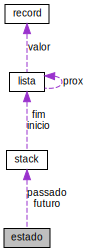
\includegraphics[width=160pt]{structestado__coll__graph}
\end{center}
\end{figure}
\subsection*{Public Attributes}
\begin{DoxyCompactItemize}
\item 
char \hyperlink{structestado_a256854b71f528cf0aafb9acb84fac759}{user} \mbox{[}\hyperlink{estado_8h_aa87360d2dd1fd5a07f92c6afe93045fc}{M\+A\+X\+\_\+\+U\+S\+E\+R}\mbox{]}
\item 
int \hyperlink{structestado_ab02e4fe5644c3b59088d7c4566d70105}{num\+\_\+lins}
\item 
int \hyperlink{structestado_a5b68d5d6aae41b5b7dd9308e40d53506}{num\+\_\+cols}
\item 
int \hyperlink{structestado_a6786d825e542118c5d79b852ace947f7}{flag}
\item 
int \hyperlink{structestado_a219ca4fd4c068f749afedb392e3f83b0}{menu}
\item 
int \hyperlink{structestado_a488c0d087dcc7e84034cdd814cf3bf3b}{help}
\item 
int \hyperlink{structestado_a87d1b6f5a4c37f8d9348c30bbf1f67cc}{wins}
\item 
char \hyperlink{structestado_a7d72f243f07d0d277f24e15e28a9a7b2}{grelha} \mbox{[}\hyperlink{estado_8h_ab02e1c5c6948bf8cf3c21a0acad8a578}{M\+A\+X\+\_\+\+G\+R\+I\+D}\mbox{]}\mbox{[}\hyperlink{estado_8h_ab02e1c5c6948bf8cf3c21a0acad8a578}{M\+A\+X\+\_\+\+G\+R\+I\+D}\mbox{]}
\item 
\hyperlink{stack_8c_a4b4ce005aaf46d538cc28d07482e137e}{S\+T\+A\+C\+K} \hyperlink{structestado_ada4a7610a6125feea84f1eeb0ae4fd1a}{passado}
\item 
\hyperlink{stack_8c_a4b4ce005aaf46d538cc28d07482e137e}{S\+T\+A\+C\+K} \hyperlink{structestado_af5d593ebecd3046a3df69b1ddec6942f}{futuro}
\end{DoxyCompactItemize}


\subsection{Detailed Description}
Estrutura que armazena o estado do jogo. 

\subsection{Member Data Documentation}
\hypertarget{structestado_a6786d825e542118c5d79b852ace947f7}{\index{estado@{estado}!flag@{flag}}
\index{flag@{flag}!estado@{estado}}
\subsubsection[{flag}]{\setlength{\rightskip}{0pt plus 5cm}int estado\+::flag}}\label{structestado_a6786d825e542118c5d79b852ace947f7}
Flag \hypertarget{structestado_af5d593ebecd3046a3df69b1ddec6942f}{\index{estado@{estado}!futuro@{futuro}}
\index{futuro@{futuro}!estado@{estado}}
\subsubsection[{futuro}]{\setlength{\rightskip}{0pt plus 5cm}{\bf S\+T\+A\+C\+K} estado\+::futuro}}\label{structestado_af5d593ebecd3046a3df69b1ddec6942f}
Stack para redo \hypertarget{structestado_a7d72f243f07d0d277f24e15e28a9a7b2}{\index{estado@{estado}!grelha@{grelha}}
\index{grelha@{grelha}!estado@{estado}}
\subsubsection[{grelha}]{\setlength{\rightskip}{0pt plus 5cm}char estado\+::grelha\mbox{[}{\bf M\+A\+X\+\_\+\+G\+R\+I\+D}\mbox{]}\mbox{[}{\bf M\+A\+X\+\_\+\+G\+R\+I\+D}\mbox{]}}}\label{structestado_a7d72f243f07d0d277f24e15e28a9a7b2}
Grelha do jogo \hypertarget{structestado_a488c0d087dcc7e84034cdd814cf3bf3b}{\index{estado@{estado}!help@{help}}
\index{help@{help}!estado@{estado}}
\subsubsection[{help}]{\setlength{\rightskip}{0pt plus 5cm}int estado\+::help}}\label{structestado_a488c0d087dcc7e84034cdd814cf3bf3b}
Número restante de hints \hypertarget{structestado_a219ca4fd4c068f749afedb392e3f83b0}{\index{estado@{estado}!menu@{menu}}
\index{menu@{menu}!estado@{estado}}
\subsubsection[{menu}]{\setlength{\rightskip}{0pt plus 5cm}int estado\+::menu}}\label{structestado_a219ca4fd4c068f749afedb392e3f83b0}
Menu atual \hypertarget{structestado_a5b68d5d6aae41b5b7dd9308e40d53506}{\index{estado@{estado}!num\+\_\+cols@{num\+\_\+cols}}
\index{num\+\_\+cols@{num\+\_\+cols}!estado@{estado}}
\subsubsection[{num\+\_\+cols}]{\setlength{\rightskip}{0pt plus 5cm}int estado\+::num\+\_\+cols}}\label{structestado_a5b68d5d6aae41b5b7dd9308e40d53506}
Número de colunas \hypertarget{structestado_ab02e4fe5644c3b59088d7c4566d70105}{\index{estado@{estado}!num\+\_\+lins@{num\+\_\+lins}}
\index{num\+\_\+lins@{num\+\_\+lins}!estado@{estado}}
\subsubsection[{num\+\_\+lins}]{\setlength{\rightskip}{0pt plus 5cm}int estado\+::num\+\_\+lins}}\label{structestado_ab02e4fe5644c3b59088d7c4566d70105}
Número de linhas \hypertarget{structestado_ada4a7610a6125feea84f1eeb0ae4fd1a}{\index{estado@{estado}!passado@{passado}}
\index{passado@{passado}!estado@{estado}}
\subsubsection[{passado}]{\setlength{\rightskip}{0pt plus 5cm}{\bf S\+T\+A\+C\+K} estado\+::passado}}\label{structestado_ada4a7610a6125feea84f1eeb0ae4fd1a}
Stack para undo \hypertarget{structestado_a256854b71f528cf0aafb9acb84fac759}{\index{estado@{estado}!user@{user}}
\index{user@{user}!estado@{estado}}
\subsubsection[{user}]{\setlength{\rightskip}{0pt plus 5cm}char estado\+::user\mbox{[}{\bf M\+A\+X\+\_\+\+U\+S\+E\+R}\mbox{]}}}\label{structestado_a256854b71f528cf0aafb9acb84fac759}
Nome de utilizador \hypertarget{structestado_a87d1b6f5a4c37f8d9348c30bbf1f67cc}{\index{estado@{estado}!wins@{wins}}
\index{wins@{wins}!estado@{estado}}
\subsubsection[{wins}]{\setlength{\rightskip}{0pt plus 5cm}int estado\+::wins}}\label{structestado_a87d1b6f5a4c37f8d9348c30bbf1f67cc}
Número de vitórias 

The documentation for this struct was generated from the following file\+:\begin{DoxyCompactItemize}
\item 
\hyperlink{estado_8c}{estado.\+c}\end{DoxyCompactItemize}

\hypertarget{structgtree}{\section{gtree Struct Reference}
\label{structgtree}\index{gtree@{gtree}}
}


Estrutura que representa o espaço de soluções de um dado Estado.  




Collaboration diagram for gtree\+:
\nopagebreak
\begin{figure}[H]
\begin{center}
\leavevmode
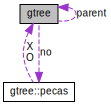
\includegraphics[width=183pt]{structgtree__coll__graph}
\end{center}
\end{figure}
\subsection*{Classes}
\begin{DoxyCompactItemize}
\item 
struct \hyperlink{structgtree_1_1pecas}{pecas}
\begin{DoxyCompactList}\small\item\em Estrutura que contem apontadores para os filhos do nodo. \end{DoxyCompactList}\end{DoxyCompactItemize}
\subsection*{Public Attributes}
\begin{DoxyCompactItemize}
\item 
int \hyperlink{structgtree_aa846f96e7fe88d420efe940ba26600b1}{side}
\item 
struct \hyperlink{structgtree_1_1pecas}{gtree\+::pecas} \hyperlink{structgtree_a9f38e15f251baa31c64e318434d17b0a}{no}
\item 
int \hyperlink{structgtree_a0eb754f1a6a1ffb0318bf6a37cdabba1}{value}
\item 
int \hyperlink{structgtree_adc3b4827f553f4791f357b0dfa35909c}{i}
\item 
int \hyperlink{structgtree_a27e5ef16fc462e2cc8a22f32ed74c4d7}{j}
\item 
struct \hyperlink{structgtree}{gtree} $\ast$ \hyperlink{structgtree_ac1cb61353a3071797136ae875d897c8d}{parent}
\end{DoxyCompactItemize}


\subsection{Detailed Description}
Estrutura que representa o espaço de soluções de um dado Estado. 

\subsection{Member Data Documentation}
\hypertarget{structgtree_adc3b4827f553f4791f357b0dfa35909c}{\index{gtree@{gtree}!i@{i}}
\index{i@{i}!gtree@{gtree}}
\subsubsection[{i}]{\setlength{\rightskip}{0pt plus 5cm}int gtree\+::i}}\label{structgtree_adc3b4827f553f4791f357b0dfa35909c}
Linha da peca. \hypertarget{structgtree_a27e5ef16fc462e2cc8a22f32ed74c4d7}{\index{gtree@{gtree}!j@{j}}
\index{j@{j}!gtree@{gtree}}
\subsubsection[{j}]{\setlength{\rightskip}{0pt plus 5cm}int gtree\+::j}}\label{structgtree_a27e5ef16fc462e2cc8a22f32ed74c4d7}
Coluna da peca. \hypertarget{structgtree_a9f38e15f251baa31c64e318434d17b0a}{\index{gtree@{gtree}!no@{no}}
\index{no@{no}!gtree@{gtree}}
\subsubsection[{no}]{\setlength{\rightskip}{0pt plus 5cm}struct {\bf gtree\+::pecas}  gtree\+::no}}\label{structgtree_a9f38e15f251baa31c64e318434d17b0a}
Estrutura para armazenar filhos do nodo. \hypertarget{structgtree_ac1cb61353a3071797136ae875d897c8d}{\index{gtree@{gtree}!parent@{parent}}
\index{parent@{parent}!gtree@{gtree}}
\subsubsection[{parent}]{\setlength{\rightskip}{0pt plus 5cm}struct {\bf gtree}$\ast$ gtree\+::parent}}\label{structgtree_ac1cb61353a3071797136ae875d897c8d}
Apontador para o nodo anterior na árvore. \hypertarget{structgtree_aa846f96e7fe88d420efe940ba26600b1}{\index{gtree@{gtree}!side@{side}}
\index{side@{side}!gtree@{gtree}}
\subsubsection[{side}]{\setlength{\rightskip}{0pt plus 5cm}int gtree\+::side}}\label{structgtree_aa846f96e7fe88d420efe940ba26600b1}
Tipo de nodo da gtree. \hypertarget{structgtree_a0eb754f1a6a1ffb0318bf6a37cdabba1}{\index{gtree@{gtree}!value@{value}}
\index{value@{value}!gtree@{gtree}}
\subsubsection[{value}]{\setlength{\rightskip}{0pt plus 5cm}int gtree\+::value}}\label{structgtree_a0eb754f1a6a1ffb0318bf6a37cdabba1}
Valor presente na peca. 

The documentation for this struct was generated from the following file\+:\begin{DoxyCompactItemize}
\item 
\hyperlink{solver_8c}{solver.\+c}\end{DoxyCompactItemize}

\hypertarget{structinfo}{\section{info Struct Reference}
\label{structinfo}\index{info@{info}}
}


Estrutura onde é guardada a informação usada pela leaderboard.  


\subsection*{Public Attributes}
\begin{DoxyCompactItemize}
\item 
int \hyperlink{structinfo_a49e18be35314982e0766370359d1ffc7}{wins}
\item 
char \hyperlink{structinfo_a5ebd1a7dd2659a6f2dc02813f223774e}{user} \mbox{[}\hyperlink{leaderboard_8h_ab5c9e28069b9fbddd9c296f14d25b84c}{M\+A\+X\+\_\+\+S}\mbox{]}
\end{DoxyCompactItemize}


\subsection{Detailed Description}
Estrutura onde é guardada a informação usada pela leaderboard. 

\subsection{Member Data Documentation}
\hypertarget{structinfo_a5ebd1a7dd2659a6f2dc02813f223774e}{\index{info@{info}!user@{user}}
\index{user@{user}!info@{info}}
\subsubsection[{user}]{\setlength{\rightskip}{0pt plus 5cm}char info\+::user\mbox{[}{\bf M\+A\+X\+\_\+\+S}\mbox{]}}}\label{structinfo_a5ebd1a7dd2659a6f2dc02813f223774e}
Utilizador guardado. \hypertarget{structinfo_a49e18be35314982e0766370359d1ffc7}{\index{info@{info}!wins@{wins}}
\index{wins@{wins}!info@{info}}
\subsubsection[{wins}]{\setlength{\rightskip}{0pt plus 5cm}int info\+::wins}}\label{structinfo_a49e18be35314982e0766370359d1ffc7}
Número de vitórias guardadas. 

The documentation for this struct was generated from the following file\+:\begin{DoxyCompactItemize}
\item 
\hyperlink{leaderboard_8c}{leaderboard.\+c}\end{DoxyCompactItemize}

\hypertarget{structlista}{\section{lista Struct Reference}
\label{structlista}\index{lista@{lista}}
}


Estrutura para a lista ligada.  




Collaboration diagram for lista\+:
\nopagebreak
\begin{figure}[H]
\begin{center}
\leavevmode
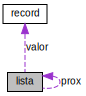
\includegraphics[width=158pt]{structlista__coll__graph}
\end{center}
\end{figure}
\subsection*{Public Attributes}
\begin{DoxyCompactItemize}
\item 
\hyperlink{stack_8c_a44e8f2943831641ea8ac9a833b65f08c}{R\+E\+C\+O\+R\+D} \hyperlink{structlista_a852a031ffa1734cf1750f54248f70bba}{valor}
\item 
struct \hyperlink{structlista}{lista} $\ast$ \hyperlink{structlista_a3b0e375147c1163d74544fd206a1f1de}{prox}
\end{DoxyCompactItemize}


\subsection{Detailed Description}
Estrutura para a lista ligada. 

\subsection{Member Data Documentation}
\hypertarget{structlista_a3b0e375147c1163d74544fd206a1f1de}{\index{lista@{lista}!prox@{prox}}
\index{prox@{prox}!lista@{lista}}
\subsubsection[{prox}]{\setlength{\rightskip}{0pt plus 5cm}struct {\bf lista}$\ast$ lista\+::prox}}\label{structlista_a3b0e375147c1163d74544fd206a1f1de}
apontador para o próximo elemento \hypertarget{structlista_a852a031ffa1734cf1750f54248f70bba}{\index{lista@{lista}!valor@{valor}}
\index{valor@{valor}!lista@{lista}}
\subsubsection[{valor}]{\setlength{\rightskip}{0pt plus 5cm}{\bf R\+E\+C\+O\+R\+D} lista\+::valor}}\label{structlista_a852a031ffa1734cf1750f54248f70bba}
valor a armazenar 

The documentation for this struct was generated from the following file\+:\begin{DoxyCompactItemize}
\item 
\hyperlink{stack_8c}{stack.\+c}\end{DoxyCompactItemize}

\hypertarget{structgtree_1_1pecas}{\section{gtree\+:\+:pecas Struct Reference}
\label{structgtree_1_1pecas}\index{gtree\+::pecas@{gtree\+::pecas}}
}


Estrutura que contem apontadores para os filhos do nodo.  




Collaboration diagram for gtree\+:\+:pecas\+:
\nopagebreak
\begin{figure}[H]
\begin{center}
\leavevmode
\includegraphics[width=183pt]{structgtree_1_1pecas__coll__graph}
\end{center}
\end{figure}
\subsection*{Public Attributes}
\begin{DoxyCompactItemize}
\item 
struct \hyperlink{structgtree}{gtree} $\ast$ \hyperlink{structgtree_1_1pecas_a91807e036e47beeb03a1868267d9ae58}{X}
\item 
struct \hyperlink{structgtree}{gtree} $\ast$ \hyperlink{structgtree_1_1pecas_a7ca95b444632a7083c1a4ff3a79662a2}{O}
\end{DoxyCompactItemize}


\subsection{Detailed Description}
Estrutura que contem apontadores para os filhos do nodo. 

\subsection{Member Data Documentation}
\hypertarget{structgtree_1_1pecas_a7ca95b444632a7083c1a4ff3a79662a2}{\index{gtree\+::pecas@{gtree\+::pecas}!O@{O}}
\index{O@{O}!gtree\+::pecas@{gtree\+::pecas}}
\subsubsection[{O}]{\setlength{\rightskip}{0pt plus 5cm}struct {\bf gtree}$\ast$ gtree\+::pecas\+::\+O}}\label{structgtree_1_1pecas_a7ca95b444632a7083c1a4ff3a79662a2}
Apontador para um filho do nodo. \hypertarget{structgtree_1_1pecas_a91807e036e47beeb03a1868267d9ae58}{\index{gtree\+::pecas@{gtree\+::pecas}!X@{X}}
\index{X@{X}!gtree\+::pecas@{gtree\+::pecas}}
\subsubsection[{X}]{\setlength{\rightskip}{0pt plus 5cm}struct {\bf gtree}$\ast$ gtree\+::pecas\+::\+X}}\label{structgtree_1_1pecas_a91807e036e47beeb03a1868267d9ae58}
Apontador para um filho do nodo. 

The documentation for this struct was generated from the following file\+:\begin{DoxyCompactItemize}
\item 
\hyperlink{solver_8c}{solver.\+c}\end{DoxyCompactItemize}

\hypertarget{structrecord}{\section{record Struct Reference}
\label{structrecord}\index{record@{record}}
}


Estrutura para o valor a armazenar.  


\subsection*{Public Attributes}
\begin{DoxyCompactItemize}
\item 
int \hyperlink{structrecord_ac301c80bc2c4273893b6d0b1045ebe4d}{i}
\item 
int \hyperlink{structrecord_a2c7b952c343a645f913aba063ac6bd8a}{j}
\item 
char \hyperlink{structrecord_a125d17b59037591de0a682688802f670}{val}
\item 
char \hyperlink{structrecord_a381a80a513768c3eba6b765c5e356bad}{check}
\end{DoxyCompactItemize}


\subsection{Detailed Description}
Estrutura para o valor a armazenar. 

\subsection{Member Data Documentation}
\hypertarget{structrecord_a381a80a513768c3eba6b765c5e356bad}{\index{record@{record}!check@{check}}
\index{check@{check}!record@{record}}
\subsubsection[{check}]{\setlength{\rightskip}{0pt plus 5cm}char record\+::check}}\label{structrecord_a381a80a513768c3eba6b765c5e356bad}
valor indicativo da âncora \hypertarget{structrecord_ac301c80bc2c4273893b6d0b1045ebe4d}{\index{record@{record}!i@{i}}
\index{i@{i}!record@{record}}
\subsubsection[{i}]{\setlength{\rightskip}{0pt plus 5cm}int record\+::i}}\label{structrecord_ac301c80bc2c4273893b6d0b1045ebe4d}
abcissa a armazenar \hypertarget{structrecord_a2c7b952c343a645f913aba063ac6bd8a}{\index{record@{record}!j@{j}}
\index{j@{j}!record@{record}}
\subsubsection[{j}]{\setlength{\rightskip}{0pt plus 5cm}int record\+::j}}\label{structrecord_a2c7b952c343a645f913aba063ac6bd8a}
ordenada a armazenar \hypertarget{structrecord_a125d17b59037591de0a682688802f670}{\index{record@{record}!val@{val}}
\index{val@{val}!record@{record}}
\subsubsection[{val}]{\setlength{\rightskip}{0pt plus 5cm}char record\+::val}}\label{structrecord_a125d17b59037591de0a682688802f670}
valor 

The documentation for this struct was generated from the following file\+:\begin{DoxyCompactItemize}
\item 
\hyperlink{stack_8c}{stack.\+c}\end{DoxyCompactItemize}

\hypertarget{structstack}{\section{stack Struct Reference}
\label{structstack}\index{stack@{stack}}
}


Declaração da Estrutura principal.  




Collaboration diagram for stack\+:
\nopagebreak
\begin{figure}[H]
\begin{center}
\leavevmode
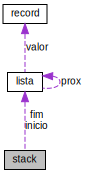
\includegraphics[width=158pt]{structstack__coll__graph}
\end{center}
\end{figure}
\subsection*{Public Attributes}
\begin{DoxyCompactItemize}
\item 
int \hyperlink{structstack_a926a597bae913d1bf4772be35c14b71e}{size}
\item 
\hyperlink{stack_8c_ab3843315393c74d2ade69877ac22d661}{L\+Rec} $\ast$ \hyperlink{structstack_ab847cafd4234504d5eed198cf88cbbf8}{inicio}
\item 
\hyperlink{stack_8c_ab3843315393c74d2ade69877ac22d661}{L\+Rec} $\ast$ \hyperlink{structstack_a802d8229341bbd71d5ef20c499753070}{fim}
\end{DoxyCompactItemize}


\subsection{Detailed Description}
Declaração da Estrutura principal. 

\subsection{Member Data Documentation}
\hypertarget{structstack_a802d8229341bbd71d5ef20c499753070}{\index{stack@{stack}!fim@{fim}}
\index{fim@{fim}!stack@{stack}}
\subsubsection[{fim}]{\setlength{\rightskip}{0pt plus 5cm}{\bf L\+Rec}$\ast$ stack\+::fim}}\label{structstack_a802d8229341bbd71d5ef20c499753070}
apontador para o fim da stack \hypertarget{structstack_ab847cafd4234504d5eed198cf88cbbf8}{\index{stack@{stack}!inicio@{inicio}}
\index{inicio@{inicio}!stack@{stack}}
\subsubsection[{inicio}]{\setlength{\rightskip}{0pt plus 5cm}{\bf L\+Rec}$\ast$ stack\+::inicio}}\label{structstack_ab847cafd4234504d5eed198cf88cbbf8}
apontador para o inicio da stack \hypertarget{structstack_a926a597bae913d1bf4772be35c14b71e}{\index{stack@{stack}!size@{size}}
\index{size@{size}!stack@{stack}}
\subsubsection[{size}]{\setlength{\rightskip}{0pt plus 5cm}int stack\+::size}}\label{structstack_a926a597bae913d1bf4772be35c14b71e}
tamanho da stack 

The documentation for this struct was generated from the following file\+:\begin{DoxyCompactItemize}
\item 
\hyperlink{stack_8c}{stack.\+c}\end{DoxyCompactItemize}

\hypertarget{structstate}{\section{state Struct Reference}
\label{structstate}\index{state@{state}}
}


Declaração do estado interno.  


\subsection*{Public Attributes}
\begin{DoxyCompactItemize}
\item 
int $\ast$$\ast$ \hyperlink{structstate_a38d05acc88f631f12c61832a59232fb7}{grelha}
\item 
int $\ast$$\ast$ \hyperlink{structstate_afc35996998683ce23fb7921410d2f0e4}{table}
\item 
int \hyperlink{structstate_a7fd2fa9e464accceb3da4c76e2198c56}{num\+\_\+cols}
\item 
int \hyperlink{structstate_a997de7249db5ec85946483c68d0a74a0}{num\+\_\+lins}
\item 
int \hyperlink{structstate_a9e68c04f3074848d9162c2429a88876b}{sqr}
\end{DoxyCompactItemize}


\subsection{Detailed Description}
Declaração do estado interno. 

\subsection{Member Data Documentation}
\hypertarget{structstate_a38d05acc88f631f12c61832a59232fb7}{\index{state@{state}!grelha@{grelha}}
\index{grelha@{grelha}!state@{state}}
\subsubsection[{grelha}]{\setlength{\rightskip}{0pt plus 5cm}int$\ast$$\ast$ state\+::grelha}}\label{structstate_a38d05acc88f631f12c61832a59232fb7}
Grelha de valores das Peças. \hypertarget{structstate_a7fd2fa9e464accceb3da4c76e2198c56}{\index{state@{state}!num\+\_\+cols@{num\+\_\+cols}}
\index{num\+\_\+cols@{num\+\_\+cols}!state@{state}}
\subsubsection[{num\+\_\+cols}]{\setlength{\rightskip}{0pt plus 5cm}int state\+::num\+\_\+cols}}\label{structstate_a7fd2fa9e464accceb3da4c76e2198c56}
Número de colunas. \hypertarget{structstate_a997de7249db5ec85946483c68d0a74a0}{\index{state@{state}!num\+\_\+lins@{num\+\_\+lins}}
\index{num\+\_\+lins@{num\+\_\+lins}!state@{state}}
\subsubsection[{num\+\_\+lins}]{\setlength{\rightskip}{0pt plus 5cm}int state\+::num\+\_\+lins}}\label{structstate_a997de7249db5ec85946483c68d0a74a0}
Número de linhas. \hypertarget{structstate_a9e68c04f3074848d9162c2429a88876b}{\index{state@{state}!sqr@{sqr}}
\index{sqr@{sqr}!state@{state}}
\subsubsection[{sqr}]{\setlength{\rightskip}{0pt plus 5cm}int state\+::sqr}}\label{structstate_a9e68c04f3074848d9162c2429a88876b}
Tamanho do lado do tabuleiro. \hypertarget{structstate_afc35996998683ce23fb7921410d2f0e4}{\index{state@{state}!table@{table}}
\index{table@{table}!state@{state}}
\subsubsection[{table}]{\setlength{\rightskip}{0pt plus 5cm}int$\ast$$\ast$ state\+::table}}\label{structstate_afc35996998683ce23fb7921410d2f0e4}
Tabela de valores das posições alteráveis. 

The documentation for this struct was generated from the following file\+:\begin{DoxyCompactItemize}
\item 
\hyperlink{solver_8c}{solver.\+c}\end{DoxyCompactItemize}

\chapter{File Documentation}
\hypertarget{cgi_8h}{\section{cgi.\+h File Reference}
\label{cgi_8h}\index{cgi.\+h@{cgi.\+h}}
}


Macros úteis para gerar C\+G\+Is.  


{\ttfamily \#include $<$stdio.\+h$>$}\\*
Include dependency graph for cgi.\+h\+:
\nopagebreak
\begin{figure}[H]
\begin{center}
\leavevmode
\includegraphics[width=126pt]{cgi_8h__incl}
\end{center}
\end{figure}
This graph shows which files directly or indirectly include this file\+:
\nopagebreak
\begin{figure}[H]
\begin{center}
\leavevmode
\includegraphics[width=350pt]{cgi_8h__dep__incl}
\end{center}
\end{figure}
\subsection*{Macros}
\begin{DoxyCompactItemize}
\item 
\#define \hyperlink{cgi_8h_a6852d85bc96a09e605bbf4a2dcfc7a5c}{I\+M\+A\+G\+E\+\_\+\+P\+A\+T\+H}~\char`\"{}http\+://localhost/images/\char`\"{}
\item 
\#define \hyperlink{cgi_8h_a58796548ab1719170bdc7cc4f6f06ea2}{A\+N\+C\+\_\+\+P\+A\+T\+H}~\char`\"{}/var/www/html/ficheiro/ancora.\+save\char`\"{}
\item 
\#define \hyperlink{cgi_8h_af783caa0ab3eaa291b0af58fcb59d2b3}{F\+I\+L\+E\+\_\+\+P\+A\+T\+H}~\char`\"{}/var/www/html/ficheiro/mapas/selectedmap.\+map\char`\"{}
\item 
\#define \hyperlink{cgi_8h_adb6f101173bcdff98b8a834cdd97fe65}{C\+H\+E\+C\+K\+\_\+\+P\+A\+T\+H}~\char`\"{}/var/www/html/ficheiro/checkpoint.\+save\char`\"{}
\item 
\#define \hyperlink{cgi_8h_a4428b4276eab18b249d924c4398f95bb}{L\+A\+S\+T\+\_\+\+P\+A\+T\+H}~\char`\"{}/var/www/html/ficheiro/last.\+save\char`\"{}
\item 
\#define \hyperlink{cgi_8h_a2997e8baab88fb20ec0dce822d405aa9}{U\+S\+E\+R\+\_\+\+P\+A\+T\+H}~\char`\"{}/usr/local/games/Ganda\+Galo/users/\char`\"{}
\item 
\#define \hyperlink{cgi_8h_a57f243883cb0b226e5af5ec6ceea763b}{M\+A\+P\+\_\+\+P\+A\+T\+H}~\char`\"{}/var/www/html/ficheiro/mapas/\char`\"{}
\item 
\hypertarget{cgi_8h_a93e071e1d9a809e4b5f9487700c40fd8}{\#define \hyperlink{cgi_8h_a93e071e1d9a809e4b5f9487700c40fd8}{C\+O\+M\+E\+C\+A\+R\+\_\+\+H\+T\+M\+L}~printf(\char`\"{}Content-\/Type\+: text/html\textbackslash{}n\textbackslash{}n$<$html$>$\textbackslash{}n\char`\"{})}\label{cgi_8h_a93e071e1d9a809e4b5f9487700c40fd8}

\begin{DoxyCompactList}\small\item\em Macro para começar o html. \end{DoxyCompactList}\item 
\#define \hyperlink{cgi_8h_add6922252041c96ce305ff5254b816f6}{A\+B\+R\+I\+R\+\_\+\+S\+V\+G}(tamx, tamy)~printf(\char`\"{}$<$svg width=\%d height=\%d style='text-\/align\+:center;'$>$\textbackslash{}n\char`\"{},tamx, tamy)
\begin{DoxyCompactList}\small\item\em Macro para abrir um svg. \end{DoxyCompactList}\item 
\hypertarget{cgi_8h_a0644b71faea318f82651ca1b25db4737}{\#define \hyperlink{cgi_8h_a0644b71faea318f82651ca1b25db4737}{F\+E\+C\+H\+A\+R\+\_\+\+S\+V\+G}~printf(\char`\"{}$<$/svg$>$\textbackslash{}n\char`\"{})}\label{cgi_8h_a0644b71faea318f82651ca1b25db4737}

\begin{DoxyCompactList}\small\item\em Macro para fechar um svg. \end{DoxyCompactList}\item 
\#define \hyperlink{cgi_8h_ab723ae3d4297ea0eb77cf3130ab15d42}{I\+M\+A\+G\+E\+M}(X, Y, E\+S\+C\+A\+L\+A, F\+I\+C\+H\+E\+I\+R\+O)
\begin{DoxyCompactList}\small\item\em Macro para criar uma imagem. \end{DoxyCompactList}\item 
\#define \hyperlink{cgi_8h_a1ae379b260243788ce152a7b87ec0e03}{Q\+U\+A\+D\+R\+A\+D\+O}(X, Y, E\+S\+C\+A\+L\+A, C\+O\+R)
\begin{DoxyCompactList}\small\item\em Macro para criar um quadrado. \end{DoxyCompactList}\item 
\#define \hyperlink{cgi_8h_a752638dcf71c9454bbac9ec8169553b0}{T\+E\+X\+T}(X, Y, C\+O\+R, text)
\begin{DoxyCompactList}\small\item\em Macro para escrever texto no ecrã \end{DoxyCompactList}\item 
\#define \hyperlink{cgi_8h_a4d82e0c3156f2bab2f120d251470623a}{A\+B\+R\+I\+R\+\_\+\+L\+I\+N\+K}(link)~printf(\char`\"{}$<$a xlink\+:href=\%s$>$\textbackslash{}n\char`\"{}, link)
\begin{DoxyCompactList}\small\item\em Macro para abrir um link. \end{DoxyCompactList}\item 
\hypertarget{cgi_8h_ae69156d6ba1d240d0660fe831f683958}{\#define \hyperlink{cgi_8h_ae69156d6ba1d240d0660fe831f683958}{F\+E\+C\+H\+A\+R\+\_\+\+L\+I\+N\+K}~printf(\char`\"{}$<$/a$>$\textbackslash{}n\char`\"{})}\label{cgi_8h_ae69156d6ba1d240d0660fe831f683958}

\begin{DoxyCompactList}\small\item\em Macro para fechar o link. \end{DoxyCompactList}\item 
\hypertarget{cgi_8h_a19f6329e29338f04cb3ddbbf235ffae6}{\#define \hyperlink{cgi_8h_a19f6329e29338f04cb3ddbbf235ffae6}{F\+E\+C\+H\+A\+R\+\_\+\+H\+T\+M\+L}~printf(\char`\"{}$<$/html$>$\textbackslash{}n\char`\"{})}\label{cgi_8h_a19f6329e29338f04cb3ddbbf235ffae6}

\begin{DoxyCompactList}\small\item\em Macro para fechar o html. \end{DoxyCompactList}\end{DoxyCompactItemize}


\subsection{Detailed Description}
Macros úteis para gerar C\+G\+Is. 



\subsection{Macro Definition Documentation}
\hypertarget{cgi_8h_a4d82e0c3156f2bab2f120d251470623a}{\index{cgi.\+h@{cgi.\+h}!A\+B\+R\+I\+R\+\_\+\+L\+I\+N\+K@{A\+B\+R\+I\+R\+\_\+\+L\+I\+N\+K}}
\index{A\+B\+R\+I\+R\+\_\+\+L\+I\+N\+K@{A\+B\+R\+I\+R\+\_\+\+L\+I\+N\+K}!cgi.\+h@{cgi.\+h}}
\subsubsection[{A\+B\+R\+I\+R\+\_\+\+L\+I\+N\+K}]{\setlength{\rightskip}{0pt plus 5cm}\#define A\+B\+R\+I\+R\+\_\+\+L\+I\+N\+K(
\begin{DoxyParamCaption}
\item[{}]{link}
\end{DoxyParamCaption}
)~printf(\char`\"{}$<$a xlink\+:href=\%s$>$\textbackslash{}n\char`\"{}, link)}}\label{cgi_8h_a4d82e0c3156f2bab2f120d251470623a}


Macro para abrir um link. 


\begin{DoxyParams}{Parameters}
{\em link} & O caminho para o link \\
\hline
\end{DoxyParams}
\hypertarget{cgi_8h_add6922252041c96ce305ff5254b816f6}{\index{cgi.\+h@{cgi.\+h}!A\+B\+R\+I\+R\+\_\+\+S\+V\+G@{A\+B\+R\+I\+R\+\_\+\+S\+V\+G}}
\index{A\+B\+R\+I\+R\+\_\+\+S\+V\+G@{A\+B\+R\+I\+R\+\_\+\+S\+V\+G}!cgi.\+h@{cgi.\+h}}
\subsubsection[{A\+B\+R\+I\+R\+\_\+\+S\+V\+G}]{\setlength{\rightskip}{0pt plus 5cm}\#define A\+B\+R\+I\+R\+\_\+\+S\+V\+G(
\begin{DoxyParamCaption}
\item[{}]{tamx, }
\item[{}]{tamy}
\end{DoxyParamCaption}
)~printf(\char`\"{}$<$svg width=\%d height=\%d style='text-\/align\+:center;'$>$\textbackslash{}n\char`\"{},tamx, tamy)}}\label{cgi_8h_add6922252041c96ce305ff5254b816f6}


Macro para abrir um svg. 


\begin{DoxyParams}{Parameters}
{\em tamx} & O comprimento do svg \\
\hline
{\em tamy} & A altura do svg \\
\hline
\end{DoxyParams}
\hypertarget{cgi_8h_a58796548ab1719170bdc7cc4f6f06ea2}{\index{cgi.\+h@{cgi.\+h}!A\+N\+C\+\_\+\+P\+A\+T\+H@{A\+N\+C\+\_\+\+P\+A\+T\+H}}
\index{A\+N\+C\+\_\+\+P\+A\+T\+H@{A\+N\+C\+\_\+\+P\+A\+T\+H}!cgi.\+h@{cgi.\+h}}
\subsubsection[{A\+N\+C\+\_\+\+P\+A\+T\+H}]{\setlength{\rightskip}{0pt plus 5cm}\#define A\+N\+C\+\_\+\+P\+A\+T\+H~\char`\"{}/var/www/html/ficheiro/ancora.\+save\char`\"{}}}\label{cgi_8h_a58796548ab1719170bdc7cc4f6f06ea2}
Caminho para as ancoras \hypertarget{cgi_8h_adb6f101173bcdff98b8a834cdd97fe65}{\index{cgi.\+h@{cgi.\+h}!C\+H\+E\+C\+K\+\_\+\+P\+A\+T\+H@{C\+H\+E\+C\+K\+\_\+\+P\+A\+T\+H}}
\index{C\+H\+E\+C\+K\+\_\+\+P\+A\+T\+H@{C\+H\+E\+C\+K\+\_\+\+P\+A\+T\+H}!cgi.\+h@{cgi.\+h}}
\subsubsection[{C\+H\+E\+C\+K\+\_\+\+P\+A\+T\+H}]{\setlength{\rightskip}{0pt plus 5cm}\#define C\+H\+E\+C\+K\+\_\+\+P\+A\+T\+H~\char`\"{}/var/www/html/ficheiro/checkpoint.\+save\char`\"{}}}\label{cgi_8h_adb6f101173bcdff98b8a834cdd97fe65}
Caminho para chekpoints \hypertarget{cgi_8h_af783caa0ab3eaa291b0af58fcb59d2b3}{\index{cgi.\+h@{cgi.\+h}!F\+I\+L\+E\+\_\+\+P\+A\+T\+H@{F\+I\+L\+E\+\_\+\+P\+A\+T\+H}}
\index{F\+I\+L\+E\+\_\+\+P\+A\+T\+H@{F\+I\+L\+E\+\_\+\+P\+A\+T\+H}!cgi.\+h@{cgi.\+h}}
\subsubsection[{F\+I\+L\+E\+\_\+\+P\+A\+T\+H}]{\setlength{\rightskip}{0pt plus 5cm}\#define F\+I\+L\+E\+\_\+\+P\+A\+T\+H~\char`\"{}/var/www/html/ficheiro/mapas/selectedmap.\+map\char`\"{}}}\label{cgi_8h_af783caa0ab3eaa291b0af58fcb59d2b3}
Caminho para mapas pré-\/definidos \hypertarget{cgi_8h_a6852d85bc96a09e605bbf4a2dcfc7a5c}{\index{cgi.\+h@{cgi.\+h}!I\+M\+A\+G\+E\+\_\+\+P\+A\+T\+H@{I\+M\+A\+G\+E\+\_\+\+P\+A\+T\+H}}
\index{I\+M\+A\+G\+E\+\_\+\+P\+A\+T\+H@{I\+M\+A\+G\+E\+\_\+\+P\+A\+T\+H}!cgi.\+h@{cgi.\+h}}
\subsubsection[{I\+M\+A\+G\+E\+\_\+\+P\+A\+T\+H}]{\setlength{\rightskip}{0pt plus 5cm}\#define I\+M\+A\+G\+E\+\_\+\+P\+A\+T\+H~\char`\"{}http\+://localhost/images/\char`\"{}}}\label{cgi_8h_a6852d85bc96a09e605bbf4a2dcfc7a5c}
Caminho para as imagens \hypertarget{cgi_8h_ab723ae3d4297ea0eb77cf3130ab15d42}{\index{cgi.\+h@{cgi.\+h}!I\+M\+A\+G\+E\+M@{I\+M\+A\+G\+E\+M}}
\index{I\+M\+A\+G\+E\+M@{I\+M\+A\+G\+E\+M}!cgi.\+h@{cgi.\+h}}
\subsubsection[{I\+M\+A\+G\+E\+M}]{\setlength{\rightskip}{0pt plus 5cm}\#define I\+M\+A\+G\+E\+M(
\begin{DoxyParamCaption}
\item[{}]{X, }
\item[{}]{Y, }
\item[{}]{E\+S\+C\+A\+L\+A, }
\item[{}]{F\+I\+C\+H\+E\+I\+R\+O}
\end{DoxyParamCaption}
)}}\label{cgi_8h_ab723ae3d4297ea0eb77cf3130ab15d42}
{\bfseries Value\+:}
\begin{DoxyCode}
printf(\textcolor{stringliteral}{"<image x=%d y=%d width=%d height=%d xlink:href=%s%s />\(\backslash\)n"}, \(\backslash\)
                                                ESCALA * X, ESCALA* Y, ESCALA, ESCALA, 
      \hyperlink{cgi_8h_a6852d85bc96a09e605bbf4a2dcfc7a5c}{IMAGE\_PATH}, FICHEIRO)
\end{DoxyCode}


Macro para criar uma imagem. 


\begin{DoxyParams}{Parameters}
{\em X} & A coordenada X do canto superior esquerdo \\
\hline
{\em Y} & A coordenada Y do canto superior esquerdo \\
\hline
{\em E\+S\+C\+A\+L\+A} & A escala da imagem \\
\hline
{\em F\+I\+C\+H\+E\+I\+R\+O} & O caminho para o link do ficheiro \\
\hline
\end{DoxyParams}
\hypertarget{cgi_8h_a4428b4276eab18b249d924c4398f95bb}{\index{cgi.\+h@{cgi.\+h}!L\+A\+S\+T\+\_\+\+P\+A\+T\+H@{L\+A\+S\+T\+\_\+\+P\+A\+T\+H}}
\index{L\+A\+S\+T\+\_\+\+P\+A\+T\+H@{L\+A\+S\+T\+\_\+\+P\+A\+T\+H}!cgi.\+h@{cgi.\+h}}
\subsubsection[{L\+A\+S\+T\+\_\+\+P\+A\+T\+H}]{\setlength{\rightskip}{0pt plus 5cm}\#define L\+A\+S\+T\+\_\+\+P\+A\+T\+H~\char`\"{}/var/www/html/ficheiro/last.\+save\char`\"{}}}\label{cgi_8h_a4428b4276eab18b249d924c4398f95bb}
Caminho para a última sava \hypertarget{cgi_8h_a57f243883cb0b226e5af5ec6ceea763b}{\index{cgi.\+h@{cgi.\+h}!M\+A\+P\+\_\+\+P\+A\+T\+H@{M\+A\+P\+\_\+\+P\+A\+T\+H}}
\index{M\+A\+P\+\_\+\+P\+A\+T\+H@{M\+A\+P\+\_\+\+P\+A\+T\+H}!cgi.\+h@{cgi.\+h}}
\subsubsection[{M\+A\+P\+\_\+\+P\+A\+T\+H}]{\setlength{\rightskip}{0pt plus 5cm}\#define M\+A\+P\+\_\+\+P\+A\+T\+H~\char`\"{}/var/www/html/ficheiro/mapas/\char`\"{}}}\label{cgi_8h_a57f243883cb0b226e5af5ec6ceea763b}
Caminho para os mapas \hypertarget{cgi_8h_a1ae379b260243788ce152a7b87ec0e03}{\index{cgi.\+h@{cgi.\+h}!Q\+U\+A\+D\+R\+A\+D\+O@{Q\+U\+A\+D\+R\+A\+D\+O}}
\index{Q\+U\+A\+D\+R\+A\+D\+O@{Q\+U\+A\+D\+R\+A\+D\+O}!cgi.\+h@{cgi.\+h}}
\subsubsection[{Q\+U\+A\+D\+R\+A\+D\+O}]{\setlength{\rightskip}{0pt plus 5cm}\#define Q\+U\+A\+D\+R\+A\+D\+O(
\begin{DoxyParamCaption}
\item[{}]{X, }
\item[{}]{Y, }
\item[{}]{E\+S\+C\+A\+L\+A, }
\item[{}]{C\+O\+R}
\end{DoxyParamCaption}
)}}\label{cgi_8h_a1ae379b260243788ce152a7b87ec0e03}
{\bfseries Value\+:}
\begin{DoxyCode}
printf(\textcolor{stringliteral}{"<rect x=%d y=%d width=%d height=%d fill=%s />\(\backslash\)n"}, \(\backslash\)
                                                ESCALA * X, ESCALA* Y, ESCALA, ESCALA, COR)
\end{DoxyCode}


Macro para criar um quadrado. 


\begin{DoxyParams}{Parameters}
{\em X} & A coordenada X do canto superior esquerdo \\
\hline
{\em Y} & A coordenada Y do canto superior esquerdo \\
\hline
{\em E\+S\+C\+A\+L\+A} & A escala do quadrado \\
\hline
{\em C\+O\+R} & A cor de preenchimento do quadrado \\
\hline
\end{DoxyParams}
\hypertarget{cgi_8h_a752638dcf71c9454bbac9ec8169553b0}{\index{cgi.\+h@{cgi.\+h}!T\+E\+X\+T@{T\+E\+X\+T}}
\index{T\+E\+X\+T@{T\+E\+X\+T}!cgi.\+h@{cgi.\+h}}
\subsubsection[{T\+E\+X\+T}]{\setlength{\rightskip}{0pt plus 5cm}\#define T\+E\+X\+T(
\begin{DoxyParamCaption}
\item[{}]{X, }
\item[{}]{Y, }
\item[{}]{C\+O\+R, }
\item[{}]{text}
\end{DoxyParamCaption}
)}}\label{cgi_8h_a752638dcf71c9454bbac9ec8169553b0}
{\bfseries Value\+:}
\begin{DoxyCode}
printf(\textcolor{stringliteral}{"<text x=%d y=%d fill=%s>%s</text>\(\backslash\)n"},  \(\backslash\)
                                                X ,Y, COR,text)
\end{DoxyCode}


Macro para escrever texto no ecrã 


\begin{DoxyParams}{Parameters}
{\em X} & A coordenada X do canto superior esquerdo \\
\hline
{\em Y} & A coordenada Y do canto superior esquerdo \\
\hline
{\em C\+O\+R} & A cor de preenchimento do quadrado \\
\hline
{\em text} & o texto a escrever \\
\hline
\end{DoxyParams}
\hypertarget{cgi_8h_a2997e8baab88fb20ec0dce822d405aa9}{\index{cgi.\+h@{cgi.\+h}!U\+S\+E\+R\+\_\+\+P\+A\+T\+H@{U\+S\+E\+R\+\_\+\+P\+A\+T\+H}}
\index{U\+S\+E\+R\+\_\+\+P\+A\+T\+H@{U\+S\+E\+R\+\_\+\+P\+A\+T\+H}!cgi.\+h@{cgi.\+h}}
\subsubsection[{U\+S\+E\+R\+\_\+\+P\+A\+T\+H}]{\setlength{\rightskip}{0pt plus 5cm}\#define U\+S\+E\+R\+\_\+\+P\+A\+T\+H~\char`\"{}/usr/local/games/Ganda\+Galo/users/\char`\"{}}}\label{cgi_8h_a2997e8baab88fb20ec0dce822d405aa9}
Caminho para os utilizadores 
\hypertarget{decide_8c}{\section{decide.\+c File Reference}
\label{decide_8c}\index{decide.\+c@{decide.\+c}}
}


Módulo encarregue da interatividade com peças.  


{\ttfamily \#include $<$stdlib.\+h$>$}\\*
{\ttfamily \#include $<$stdio.\+h$>$}\\*
{\ttfamily \#include \char`\"{}estado.\+h\char`\"{}}\\*
{\ttfamily \#include \char`\"{}validate.\+h\char`\"{}}\\*
{\ttfamily \#include \char`\"{}decide.\+h\char`\"{}}\\*
Include dependency graph for decide.\+c\+:
\nopagebreak
\begin{figure}[H]
\begin{center}
\leavevmode
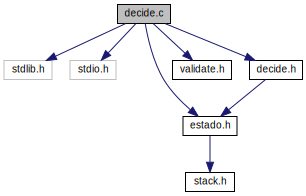
\includegraphics[width=350pt]{decide_8c__incl}
\end{center}
\end{figure}
\subsection*{Functions}
\begin{DoxyCompactItemize}
\item 
int \hyperlink{decide_8c_ae13669ac08e09c81d021c5569733e0fb}{formove} (\hyperlink{estado_8c_afbffb4e9c242f93d5a2d607754ce2db8}{E\+S\+T\+A\+D\+O} \hyperlink{structstate}{state}, int i, int j)
\begin{DoxyCompactList}\small\item\em Função que indica quantas casas devem ser avançadas de modo a manter a validade do jogo. \end{DoxyCompactList}\item 
char \hyperlink{decide_8c_a7c4586a82bbbd99e2b8f94e12b2a3535}{advance} (char num, int n, char mode)
\begin{DoxyCompactList}\small\item\em Função decide internamente que tipo de função aplicar ao avanço do jogo consoante o modo. \end{DoxyCompactList}\item 
void \hyperlink{decide_8c_a82c09231e65f427fb432011ca6e79ad1}{play\+Pos} (\hyperlink{estado_8c_afbffb4e9c242f93d5a2d607754ce2db8}{E\+S\+T\+A\+D\+O} e, int i, int j)
\begin{DoxyCompactList}\small\item\em Função que faz uma jogada no estado consoante uma de jogo e a posição. \end{DoxyCompactList}\item 
static char \hyperlink{decide_8c_a4d25df32b3ea1a2e448dd71c637f7d9d}{drawadvance} (char num, int n)
\begin{DoxyCompactList}\small\item\em Função utilizada para o avanço sucessivo de peças para o modo de desenho. \end{DoxyCompactList}\end{DoxyCompactItemize}


\subsection{Detailed Description}
Módulo encarregue da interatividade com peças. 



\subsection{Function Documentation}
\hypertarget{decide_8c_a7c4586a82bbbd99e2b8f94e12b2a3535}{\index{decide.\+c@{decide.\+c}!advance@{advance}}
\index{advance@{advance}!decide.\+c@{decide.\+c}}
\subsubsection[{advance}]{\setlength{\rightskip}{0pt plus 5cm}char advance (
\begin{DoxyParamCaption}
\item[{char}]{num, }
\item[{int}]{n, }
\item[{char}]{mode}
\end{DoxyParamCaption}
)}}\label{decide_8c_a7c4586a82bbbd99e2b8f94e12b2a3535}


Função decide internamente que tipo de função aplicar ao avanço do jogo consoante o modo. 


\begin{DoxyParams}{Parameters}
{\em num} & O valor apartir do qual se pretende avançar. \\
\hline
{\em n} & O numéro de vezes que se irá avançar. \\
\hline
{\em mode} & O modo do jogo.\\
\hline
\end{DoxyParams}
\begin{DoxyReturn}{Returns}
O valor resultante. 
\end{DoxyReturn}
\hypertarget{decide_8c_a4d25df32b3ea1a2e448dd71c637f7d9d}{\index{decide.\+c@{decide.\+c}!drawadvance@{drawadvance}}
\index{drawadvance@{drawadvance}!decide.\+c@{decide.\+c}}
\subsubsection[{drawadvance}]{\setlength{\rightskip}{0pt plus 5cm}static char drawadvance (
\begin{DoxyParamCaption}
\item[{char}]{num, }
\item[{int}]{n}
\end{DoxyParamCaption}
)\hspace{0.3cm}{\ttfamily [static]}}}\label{decide_8c_a4d25df32b3ea1a2e448dd71c637f7d9d}


Função utilizada para o avanço sucessivo de peças para o modo de desenho. 

Avança cada valor normalmente de modo a que seja possível jogar o valor B\+L\+O\+Q\+U\+E\+A\+D\+O.


\begin{DoxyParams}{Parameters}
{\em num} & O valor apartir do qual se pretende avançar. \\
\hline
{\em n} & O numéro de vezes que se irá avançar.\\
\hline
\end{DoxyParams}
\begin{DoxyReturn}{Returns}
O valor resultante. 
\end{DoxyReturn}
\hypertarget{decide_8c_ae13669ac08e09c81d021c5569733e0fb}{\index{decide.\+c@{decide.\+c}!formove@{formove}}
\index{formove@{formove}!decide.\+c@{decide.\+c}}
\subsubsection[{formove}]{\setlength{\rightskip}{0pt plus 5cm}int formove (
\begin{DoxyParamCaption}
\item[{{\bf E\+S\+T\+A\+D\+O}}]{state, }
\item[{int}]{i, }
\item[{int}]{j}
\end{DoxyParamCaption}
)}}\label{decide_8c_ae13669ac08e09c81d021c5569733e0fb}


Função que indica quantas casas devem ser avançadas de modo a manter a validade do jogo. 


\begin{DoxyParams}{Parameters}
{\em state} & Estado do qual se pretend aferir a validade. \\
\hline
{\em i} & Linha que se pretende avaliar. \\
\hline
{\em j} & Coluna que se pretende avaliar.\\
\hline
\end{DoxyParams}
\begin{DoxyReturn}{Returns}
Quantas casas deve avançar. 
\end{DoxyReturn}
\hypertarget{decide_8c_a82c09231e65f427fb432011ca6e79ad1}{\index{decide.\+c@{decide.\+c}!play\+Pos@{play\+Pos}}
\index{play\+Pos@{play\+Pos}!decide.\+c@{decide.\+c}}
\subsubsection[{play\+Pos}]{\setlength{\rightskip}{0pt plus 5cm}void play\+Pos (
\begin{DoxyParamCaption}
\item[{{\bf E\+S\+T\+A\+D\+O}}]{e, }
\item[{int}]{i, }
\item[{int}]{j}
\end{DoxyParamCaption}
)}}\label{decide_8c_a82c09231e65f427fb432011ca6e79ad1}


Função que faz uma jogada no estado consoante uma de jogo e a posição. 


\begin{DoxyParams}{Parameters}
{\em e} & Apontador para o estado que irá ser alterado. \\
\hline
{\em i} & Linha onde se pretende fazer a jogada. \\
\hline
{\em j} & Colunas onde se pretende fazer a jogada. \\
\hline
\end{DoxyParams}

\hypertarget{decide_8h}{\section{decide.\+h File Reference}
\label{decide_8h}\index{decide.\+h@{decide.\+h}}
}


Módulo encarregue da interatividade com peças.  


{\ttfamily \#include \char`\"{}estado.\+h\char`\"{}}\\*
Include dependency graph for decide.\+h\+:
\nopagebreak
\begin{figure}[H]
\begin{center}
\leavevmode
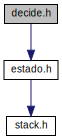
\includegraphics[width=134pt]{decide_8h__incl}
\end{center}
\end{figure}
This graph shows which files directly or indirectly include this file\+:
\nopagebreak
\begin{figure}[H]
\begin{center}
\leavevmode
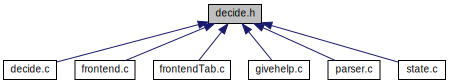
\includegraphics[width=350pt]{decide_8h__dep__incl}
\end{center}
\end{figure}
\subsection*{Macros}
\begin{DoxyCompactItemize}
\item 
\#define \hyperlink{decide_8h_ac47faeda9e29e07135095e3711035845}{playadvance}(num, n)~(((num + n) $>$ (S\+O\+L\+\_\+\+O)) ? (V\+A\+Z\+I\+A)\+:((num) + n) )
\begin{DoxyCompactList}\small\item\em Macro que indica de que foram devem progredir as peças para o modo de jogo play. \end{DoxyCompactList}\end{DoxyCompactItemize}
\subsection*{Enumerations}
\begin{DoxyCompactItemize}
\item 
\hypertarget{decide_8h_a7eabd788dcab19ca586663bf73deddf5}{enum \hyperlink{decide_8h_a7eabd788dcab19ca586663bf73deddf5}{M\+O\+D\+E} \{ {\bfseries D\+R\+A\+W}, 
{\bfseries P\+L\+A\+Y}
 \}}\label{decide_8h_a7eabd788dcab19ca586663bf73deddf5}

\begin{DoxyCompactList}\small\item\em Estrutura indicativa do modo de jogo. \end{DoxyCompactList}\end{DoxyCompactItemize}
\subsection*{Functions}
\begin{DoxyCompactItemize}
\item 
int \hyperlink{decide_8h_ae13669ac08e09c81d021c5569733e0fb}{formove} (\hyperlink{estado_8c_afbffb4e9c242f93d5a2d607754ce2db8}{E\+S\+T\+A\+D\+O} \hyperlink{structstate}{state}, int i, int j)
\begin{DoxyCompactList}\small\item\em Função que indica quantas casas devem ser avançadas de modo a manter a validade do jogo. \end{DoxyCompactList}\item 
char \hyperlink{decide_8h_a7c4586a82bbbd99e2b8f94e12b2a3535}{advance} (char num, int n, char mode)
\begin{DoxyCompactList}\small\item\em Função decide internamente que tipo de função aplicar ao avanço do jogo consoante o modo. \end{DoxyCompactList}\item 
void \hyperlink{decide_8h_a82c09231e65f427fb432011ca6e79ad1}{play\+Pos} (\hyperlink{estado_8c_afbffb4e9c242f93d5a2d607754ce2db8}{E\+S\+T\+A\+D\+O} e, int i, int j)
\begin{DoxyCompactList}\small\item\em Função que faz uma jogada no estado consoante uma de jogo e a posição. \end{DoxyCompactList}\end{DoxyCompactItemize}


\subsection{Detailed Description}
Módulo encarregue da interatividade com peças. 



\subsection{Macro Definition Documentation}
\hypertarget{decide_8h_ac47faeda9e29e07135095e3711035845}{\index{decide.\+h@{decide.\+h}!playadvance@{playadvance}}
\index{playadvance@{playadvance}!decide.\+h@{decide.\+h}}
\subsubsection[{playadvance}]{\setlength{\rightskip}{0pt plus 5cm}\#define playadvance(
\begin{DoxyParamCaption}
\item[{}]{num, }
\item[{}]{n}
\end{DoxyParamCaption}
)~(((num + n) $>$ (S\+O\+L\+\_\+\+O)) ? (V\+A\+Z\+I\+A)\+:((num) + n) )}}\label{decide_8h_ac47faeda9e29e07135095e3711035845}


Macro que indica de que foram devem progredir as peças para o modo de jogo play. 


\begin{DoxyParams}{Parameters}
{\em num} & O valor apartir do qual se pretende avançar. \\
\hline
{\em n} & O numéro de vezes que se irá avançar.\\
\hline
\end{DoxyParams}
\begin{DoxyReturn}{Returns}
o valor resultante. 
\end{DoxyReturn}


\subsection{Function Documentation}
\hypertarget{decide_8h_a7c4586a82bbbd99e2b8f94e12b2a3535}{\index{decide.\+h@{decide.\+h}!advance@{advance}}
\index{advance@{advance}!decide.\+h@{decide.\+h}}
\subsubsection[{advance}]{\setlength{\rightskip}{0pt plus 5cm}char advance (
\begin{DoxyParamCaption}
\item[{char}]{num, }
\item[{int}]{n, }
\item[{char}]{mode}
\end{DoxyParamCaption}
)}}\label{decide_8h_a7c4586a82bbbd99e2b8f94e12b2a3535}


Função decide internamente que tipo de função aplicar ao avanço do jogo consoante o modo. 


\begin{DoxyParams}{Parameters}
{\em num} & O valor apartir do qual se pretende avançar. \\
\hline
{\em n} & O numéro de vezes que se irá avançar. \\
\hline
{\em mode} & O modo do jogo.\\
\hline
\end{DoxyParams}
\begin{DoxyReturn}{Returns}
O valor resultante. 
\end{DoxyReturn}
\hypertarget{decide_8h_ae13669ac08e09c81d021c5569733e0fb}{\index{decide.\+h@{decide.\+h}!formove@{formove}}
\index{formove@{formove}!decide.\+h@{decide.\+h}}
\subsubsection[{formove}]{\setlength{\rightskip}{0pt plus 5cm}int formove (
\begin{DoxyParamCaption}
\item[{{\bf E\+S\+T\+A\+D\+O}}]{state, }
\item[{int}]{i, }
\item[{int}]{j}
\end{DoxyParamCaption}
)}}\label{decide_8h_ae13669ac08e09c81d021c5569733e0fb}


Função que indica quantas casas devem ser avançadas de modo a manter a validade do jogo. 


\begin{DoxyParams}{Parameters}
{\em state} & Estado do qual se pretend aferir a validade. \\
\hline
{\em i} & Linha que se pretende avaliar. \\
\hline
{\em j} & Coluna que se pretende avaliar.\\
\hline
\end{DoxyParams}
\begin{DoxyReturn}{Returns}
Quantas casas deve avançar. 
\end{DoxyReturn}
\hypertarget{decide_8h_a82c09231e65f427fb432011ca6e79ad1}{\index{decide.\+h@{decide.\+h}!play\+Pos@{play\+Pos}}
\index{play\+Pos@{play\+Pos}!decide.\+h@{decide.\+h}}
\subsubsection[{play\+Pos}]{\setlength{\rightskip}{0pt plus 5cm}void play\+Pos (
\begin{DoxyParamCaption}
\item[{{\bf E\+S\+T\+A\+D\+O}}]{e, }
\item[{int}]{i, }
\item[{int}]{j}
\end{DoxyParamCaption}
)}}\label{decide_8h_a82c09231e65f427fb432011ca6e79ad1}


Função que faz uma jogada no estado consoante uma de jogo e a posição. 


\begin{DoxyParams}{Parameters}
{\em e} & Apontador para o estado que irá ser alterado. \\
\hline
{\em i} & Linha onde se pretende fazer a jogada. \\
\hline
{\em j} & Colunas onde se pretende fazer a jogada. \\
\hline
\end{DoxyParams}

\hypertarget{estado_8c}{\section{estado.\+c File Reference}
\label{estado_8c}\index{estado.\+c@{estado.\+c}}
}


Ficheiro contendo o código relativo ao módulo {\ttfamily E\+S\+T\+A\+D\+O}.  


{\ttfamily \#include $<$stdlib.\+h$>$}\\*
{\ttfamily \#include $<$stdio.\+h$>$}\\*
{\ttfamily \#include $<$string.\+h$>$}\\*
{\ttfamily \#include \char`\"{}estado.\+h\char`\"{}}\\*
{\ttfamily \#include \char`\"{}cgi.\+h\char`\"{}}\\*
{\ttfamily \#include \char`\"{}frontend.\+h\char`\"{}}\\*
{\ttfamily \#include \char`\"{}filemanager.\+h\char`\"{}}\\*
{\ttfamily \#include \char`\"{}state.\+h\char`\"{}}\\*
{\ttfamily \#include \char`\"{}solver.\+h\char`\"{}}\\*
{\ttfamily \#include \char`\"{}leaderboard.\+h\char`\"{}}\\*
Include dependency graph for estado.\+c\+:
\nopagebreak
\begin{figure}[H]
\begin{center}
\leavevmode
\includegraphics[width=350pt]{estado_8c__incl}
\end{center}
\end{figure}
\subsection*{Classes}
\begin{DoxyCompactItemize}
\item 
struct \hyperlink{structestado}{estado}
\begin{DoxyCompactList}\small\item\em Estrutura que armazena o estado do jogo. \end{DoxyCompactList}\end{DoxyCompactItemize}
\subsection*{Typedefs}
\begin{DoxyCompactItemize}
\item 
\hypertarget{estado_8c_afbffb4e9c242f93d5a2d607754ce2db8}{typedef struct \hyperlink{structestado}{estado} $\ast$ \hyperlink{estado_8c_afbffb4e9c242f93d5a2d607754ce2db8}{E\+S\+T\+A\+D\+O}}\label{estado_8c_afbffb4e9c242f93d5a2d607754ce2db8}

\begin{DoxyCompactList}\small\item\em Estrutura que armazena o estado do jogo. \end{DoxyCompactList}\end{DoxyCompactItemize}
\subsection*{Functions}
\begin{DoxyCompactItemize}
\item 
\hyperlink{estado_8c_afbffb4e9c242f93d5a2d607754ce2db8}{E\+S\+T\+A\+D\+O} \hyperlink{estado_8c_a425d9a13679db6099c218938240ba30d}{make\+State} (\hyperlink{estado_8c_afbffb4e9c242f93d5a2d607754ce2db8}{E\+S\+T\+A\+D\+O} e)
\begin{DoxyCompactList}\small\item\em Função que cria um estado. \end{DoxyCompactList}\item 
void \hyperlink{estado_8c_a8b28e51aaf0dded437325daee1e86238}{destroy\+State} (\hyperlink{estado_8c_afbffb4e9c242f93d5a2d607754ce2db8}{E\+S\+T\+A\+D\+O} e)
\begin{DoxyCompactList}\small\item\em Função que destroi o estado. \end{DoxyCompactList}\item 
\hyperlink{estado_8c_afbffb4e9c242f93d5a2d607754ce2db8}{E\+S\+T\+A\+D\+O} \hyperlink{estado_8c_a1c52197ddde667791a5210fd441cd3dc}{inicializar} (char $\ast$user, int ln, int col)
\begin{DoxyCompactList}\small\item\em Função que inicializa o estado. \end{DoxyCompactList}\item 
long \hyperlink{estado_8c_adacdc0e19436cc110b84a389bda1d153}{n\+\_\+solutions} (\hyperlink{estado_8c_afbffb4e9c242f93d5a2d607754ce2db8}{E\+S\+T\+A\+D\+O} e)
\begin{DoxyCompactList}\small\item\em Função que indica o número de soluções de um tabuleiro. \end{DoxyCompactList}\item 
void \hyperlink{estado_8c_aa7a928e6dc71c7e6f4e25da3b5c10006}{set\+E\+\_\+state} (\hyperlink{estado_8c_afbffb4e9c242f93d5a2d607754ce2db8}{E\+S\+T\+A\+D\+O} dest, \hyperlink{estado_8c_afbffb4e9c242f93d5a2d607754ce2db8}{E\+S\+T\+A\+D\+O} sourc)
\begin{DoxyCompactList}\small\item\em Função que copia um estado para outro. \end{DoxyCompactList}\item 
void \hyperlink{estado_8c_ad2a155483a55076e3b583984fa4080e2}{set\+E\+\_\+user} (\hyperlink{estado_8c_afbffb4e9c242f93d5a2d607754ce2db8}{E\+S\+T\+A\+D\+O} e, char $\ast$user)
\begin{DoxyCompactList}\small\item\em Função que altera o nome de utilizador num estado. \end{DoxyCompactList}\item 
void \hyperlink{estado_8c_a409faed7da253d71a139e68c80d7c3d4}{set\+E\+\_\+lins} (\hyperlink{estado_8c_afbffb4e9c242f93d5a2d607754ce2db8}{E\+S\+T\+A\+D\+O} e, int lins)
\begin{DoxyCompactList}\small\item\em Função que altera o número de linhas. \end{DoxyCompactList}\item 
void \hyperlink{estado_8c_a5fbaea168b59397cd59b16683935a278}{set\+E\+\_\+cols} (\hyperlink{estado_8c_afbffb4e9c242f93d5a2d607754ce2db8}{E\+S\+T\+A\+D\+O} e, int cols)
\begin{DoxyCompactList}\small\item\em Função que altera o número de colunas. \end{DoxyCompactList}\item 
void \hyperlink{estado_8c_a173aba83ee9ef88015706361de32ae1d}{set\+E\+\_\+menu} (\hyperlink{estado_8c_afbffb4e9c242f93d5a2d607754ce2db8}{E\+S\+T\+A\+D\+O} e, int menu)
\begin{DoxyCompactList}\small\item\em Função que altera o menu. \end{DoxyCompactList}\item 
void \hyperlink{estado_8c_a0b2cdae45084d690be7137255dfac0cb}{set\+E\+\_\+elem} (\hyperlink{estado_8c_afbffb4e9c242f93d5a2d607754ce2db8}{E\+S\+T\+A\+D\+O} e, int i, int j, char val)
\begin{DoxyCompactList}\small\item\em Função que altera um elemento do tabuleiro. \end{DoxyCompactList}\item 
void \hyperlink{estado_8c_aae2d35f0ec536272ce5ddf4a4a4cb5e9}{set\+E\+\_\+elem\+T} (\hyperlink{estado_8c_afbffb4e9c242f93d5a2d607754ce2db8}{E\+S\+T\+A\+D\+O} e, int i, int j, char($\ast$map)(char))
\begin{DoxyCompactList}\small\item\em Altera um elemento consoante uma função mapping. \end{DoxyCompactList}\item 
void \hyperlink{estado_8c_a1cae4d8b65b1431a0a162399c8a5fdeb}{set\+E\+\_\+stack} (\hyperlink{estado_8c_afbffb4e9c242f93d5a2d607754ce2db8}{E\+S\+T\+A\+D\+O} e, \hyperlink{stack_8c_a4b4ce005aaf46d538cc28d07482e137e}{S\+T\+A\+C\+K} s, int c)
\begin{DoxyCompactList}\small\item\em Função que altera as stack no estado. \end{DoxyCompactList}\item 
void \hyperlink{estado_8c_aec99fff0cdbcf7313a220b9908396c3c}{set\+E\+\_\+flag} (\hyperlink{estado_8c_afbffb4e9c242f93d5a2d607754ce2db8}{E\+S\+T\+A\+D\+O} e, int flag)
\item 
void \hyperlink{estado_8c_ab7d13ddf2b3bdb333b271cc83eb1324e}{set\+E\+\_\+transverse} (\hyperlink{estado_8c_afbffb4e9c242f93d5a2d607754ce2db8}{E\+S\+T\+A\+D\+O} e, int li, int ci, char($\ast$map)(char))
\begin{DoxyCompactList}\small\item\em Aplica uma função de mapping a vários elementos da grelha. \end{DoxyCompactList}\item 
void \hyperlink{estado_8c_a5eff026b884b0da81f84f8658a3d850d}{set\+E\+\_\+base} (\hyperlink{estado_8c_afbffb4e9c242f93d5a2d607754ce2db8}{E\+S\+T\+A\+D\+O} e, char($\ast$map)(char))
\begin{DoxyCompactList}\small\item\em Coloca no estado indicado um base. \end{DoxyCompactList}\item 
void \hyperlink{estado_8c_a37030bdeb38ad57caa19d47f541f14f3}{set\+E\+\_\+help} (\hyperlink{estado_8c_afbffb4e9c242f93d5a2d607754ce2db8}{E\+S\+T\+A\+D\+O} e, int help)
\begin{DoxyCompactList}\small\item\em Função que altera o número de ajudas. \end{DoxyCompactList}\item 
void \hyperlink{estado_8c_ac5c132634200250bdaa5ae7a20e524c1}{set\+E\+\_\+help\+B} (\hyperlink{estado_8c_afbffb4e9c242f93d5a2d607754ce2db8}{E\+S\+T\+A\+D\+O} e)
\begin{DoxyCompactList}\small\item\em Função que coloca um número base de ajudas em {\ttfamily e} . \end{DoxyCompactList}\item 
char $\ast$ \hyperlink{estado_8c_a71766588f77acf7e8db60edf80a0f244}{get\+E\+\_\+user} (\hyperlink{estado_8c_afbffb4e9c242f93d5a2d607754ce2db8}{E\+S\+T\+A\+D\+O} e)
\begin{DoxyCompactList}\small\item\em Função que devolve o nome de utilizador. \end{DoxyCompactList}\item 
int \hyperlink{estado_8c_a4d3c25878918fa5fd1ea3d4a0b1e7a8d}{get\+E\+\_\+cols} (\hyperlink{estado_8c_afbffb4e9c242f93d5a2d607754ce2db8}{E\+S\+T\+A\+D\+O} e)
\begin{DoxyCompactList}\small\item\em Função que devolve o número de colunas na grelha. \end{DoxyCompactList}\item 
int \hyperlink{estado_8c_aa3dfd8301c50f971b2d20815617e00d3}{get\+E\+\_\+lins} (\hyperlink{estado_8c_afbffb4e9c242f93d5a2d607754ce2db8}{E\+S\+T\+A\+D\+O} e)
\begin{DoxyCompactList}\small\item\em Função que devolve o número de linhas na grelha. \end{DoxyCompactList}\item 
int \hyperlink{estado_8c_a6b89af2e2e3e9eaf3521701eec86a702}{get\+E\+\_\+menu} (\hyperlink{estado_8c_afbffb4e9c242f93d5a2d607754ce2db8}{E\+S\+T\+A\+D\+O} e)
\begin{DoxyCompactList}\small\item\em Função que devolve o menu atual. \end{DoxyCompactList}\item 
\hyperlink{stack_8c_a4b4ce005aaf46d538cc28d07482e137e}{S\+T\+A\+C\+K} \hyperlink{estado_8c_aa61011eadf880d552d197316ad4b30bb}{get\+E\+\_\+stack} (\hyperlink{estado_8c_afbffb4e9c242f93d5a2d607754ce2db8}{E\+S\+T\+A\+D\+O} e, int c)
\begin{DoxyCompactList}\small\item\em Função que devolve uma {\ttfamily S\+T\+A\+C\+K} do {\ttfamily E\+S\+T\+A\+D\+O}. \end{DoxyCompactList}\item 
int \hyperlink{estado_8c_af4fdbc1ee04d56bef9bd3fb97bb70cee}{get\+E\+\_\+flag} (\hyperlink{estado_8c_afbffb4e9c242f93d5a2d607754ce2db8}{E\+S\+T\+A\+D\+O} e)
\begin{DoxyCompactList}\small\item\em Função que devolve a {\ttfamily flag}. \end{DoxyCompactList}\item 
char \hyperlink{estado_8c_ae4aeab324373aa7d36cd03ad28caae57}{get\+E\+\_\+elem} (\hyperlink{estado_8c_afbffb4e9c242f93d5a2d607754ce2db8}{E\+S\+T\+A\+D\+O} e, int i, int j)
\begin{DoxyCompactList}\small\item\em Função que devolve um elemento da grelha. \end{DoxyCompactList}\item 
int \hyperlink{estado_8c_ab3e47d845be6ab389f1cb63532ab9313}{get\+E\+\_\+help} (\hyperlink{estado_8c_afbffb4e9c242f93d5a2d607754ce2db8}{E\+S\+T\+A\+D\+O} e)
\begin{DoxyCompactList}\small\item\em Função que devolve o número de ajudas. \end{DoxyCompactList}\item 
int \hyperlink{estado_8c_a27328d911d982f65736cd7ce9a136cfe}{get\+E\+\_\+verf} (\hyperlink{estado_8c_afbffb4e9c242f93d5a2d607754ce2db8}{E\+S\+T\+A\+D\+O} e, int($\ast$inclusivecase)(\hyperlink{estado_8c_afbffb4e9c242f93d5a2d607754ce2db8}{E\+S\+T\+A\+D\+O}, int, int))
\begin{DoxyCompactList}\small\item\em Função que verifica todas as peças de um tabuleiro. \end{DoxyCompactList}\item 
void \hyperlink{estado_8c_aba618389582d28f62b9b79f5f3f6fe48}{set\+E\+\_\+wins} (\hyperlink{estado_8c_afbffb4e9c242f93d5a2d607754ce2db8}{E\+S\+T\+A\+D\+O} e, int wins)
\begin{DoxyCompactList}\small\item\em Função que coloca o número de vitórias no {\ttfamily E\+S\+T\+A\+D\+O} e no ficheiro para tal. \end{DoxyCompactList}\item 
int \hyperlink{estado_8c_ad843d5e51766f087443787b3f2623961}{get\+E\+\_\+wins} (\hyperlink{estado_8c_afbffb4e9c242f93d5a2d607754ce2db8}{E\+S\+T\+A\+D\+O} e)
\begin{DoxyCompactList}\small\item\em Função que obtem o número de vitórias do estado. \end{DoxyCompactList}\end{DoxyCompactItemize}


\subsection{Detailed Description}
Ficheiro contendo o código relativo ao módulo {\ttfamily E\+S\+T\+A\+D\+O}. 



\subsection{Function Documentation}
\hypertarget{estado_8c_a8b28e51aaf0dded437325daee1e86238}{\index{estado.\+c@{estado.\+c}!destroy\+State@{destroy\+State}}
\index{destroy\+State@{destroy\+State}!estado.\+c@{estado.\+c}}
\subsubsection[{destroy\+State}]{\setlength{\rightskip}{0pt plus 5cm}void destroy\+State (
\begin{DoxyParamCaption}
\item[{{\bf E\+S\+T\+A\+D\+O}}]{e}
\end{DoxyParamCaption}
)}}\label{estado_8c_a8b28e51aaf0dded437325daee1e86238}


Função que destroi o estado. 


\begin{DoxyParams}{Parameters}
{\em e} & Estado a destruir. \\
\hline
\end{DoxyParams}
\hypertarget{estado_8c_a4d3c25878918fa5fd1ea3d4a0b1e7a8d}{\index{estado.\+c@{estado.\+c}!get\+E\+\_\+cols@{get\+E\+\_\+cols}}
\index{get\+E\+\_\+cols@{get\+E\+\_\+cols}!estado.\+c@{estado.\+c}}
\subsubsection[{get\+E\+\_\+cols}]{\setlength{\rightskip}{0pt plus 5cm}int get\+E\+\_\+cols (
\begin{DoxyParamCaption}
\item[{{\bf E\+S\+T\+A\+D\+O}}]{e}
\end{DoxyParamCaption}
)}}\label{estado_8c_a4d3c25878918fa5fd1ea3d4a0b1e7a8d}


Função que devolve o número de colunas na grelha. 


\begin{DoxyParams}{Parameters}
{\em e} & Estado a procurar.\\
\hline
\end{DoxyParams}
\begin{DoxyReturn}{Returns}
Número de colunas.
\end{DoxyReturn}
\begin{DoxySeeAlso}{See also}
\hyperlink{structestado_a5b68d5d6aae41b5b7dd9308e40d53506}{estado\+::num\+\_\+cols} 
\end{DoxySeeAlso}
\hypertarget{estado_8c_ae4aeab324373aa7d36cd03ad28caae57}{\index{estado.\+c@{estado.\+c}!get\+E\+\_\+elem@{get\+E\+\_\+elem}}
\index{get\+E\+\_\+elem@{get\+E\+\_\+elem}!estado.\+c@{estado.\+c}}
\subsubsection[{get\+E\+\_\+elem}]{\setlength{\rightskip}{0pt plus 5cm}char get\+E\+\_\+elem (
\begin{DoxyParamCaption}
\item[{{\bf E\+S\+T\+A\+D\+O}}]{e, }
\item[{int}]{i, }
\item[{int}]{j}
\end{DoxyParamCaption}
)}}\label{estado_8c_ae4aeab324373aa7d36cd03ad28caae57}


Função que devolve um elemento da grelha. 


\begin{DoxyParams}{Parameters}
{\em e} & Estado a procurar. \\
\hline
{\em i} & Linha do elemento. \\
\hline
{\em j} & Coluna do elemento.\\
\hline
\end{DoxyParams}
\begin{DoxyReturn}{Returns}
Elemento na linha 'i' e coluna 'j'. 
\end{DoxyReturn}
\hypertarget{estado_8c_af4fdbc1ee04d56bef9bd3fb97bb70cee}{\index{estado.\+c@{estado.\+c}!get\+E\+\_\+flag@{get\+E\+\_\+flag}}
\index{get\+E\+\_\+flag@{get\+E\+\_\+flag}!estado.\+c@{estado.\+c}}
\subsubsection[{get\+E\+\_\+flag}]{\setlength{\rightskip}{0pt plus 5cm}int get\+E\+\_\+flag (
\begin{DoxyParamCaption}
\item[{{\bf E\+S\+T\+A\+D\+O}}]{e}
\end{DoxyParamCaption}
)}}\label{estado_8c_af4fdbc1ee04d56bef9bd3fb97bb70cee}


Função que devolve a {\ttfamily flag}. 


\begin{DoxyParams}{Parameters}
{\em e} & {\ttfamily E\+S\+T\+A\+D\+O} a procurar.\\
\hline
\end{DoxyParams}
\begin{DoxyReturn}{Returns}
{\ttfamily flag} do {\ttfamily Estado}.
\end{DoxyReturn}
\begin{DoxySeeAlso}{See also}
\hyperlink{structestado_a6786d825e542118c5d79b852ace947f7}{estado\+::flag} 
\end{DoxySeeAlso}
\hypertarget{estado_8c_ab3e47d845be6ab389f1cb63532ab9313}{\index{estado.\+c@{estado.\+c}!get\+E\+\_\+help@{get\+E\+\_\+help}}
\index{get\+E\+\_\+help@{get\+E\+\_\+help}!estado.\+c@{estado.\+c}}
\subsubsection[{get\+E\+\_\+help}]{\setlength{\rightskip}{0pt plus 5cm}int get\+E\+\_\+help (
\begin{DoxyParamCaption}
\item[{{\bf E\+S\+T\+A\+D\+O}}]{e}
\end{DoxyParamCaption}
)}}\label{estado_8c_ab3e47d845be6ab389f1cb63532ab9313}


Função que devolve o número de ajudas. 


\begin{DoxyParams}{Parameters}
{\em e} & Estado a procurar.\\
\hline
\end{DoxyParams}
\begin{DoxyReturn}{Returns}
Número de ajudas.
\end{DoxyReturn}
\begin{DoxySeeAlso}{See also}
\hyperlink{structestado_a488c0d087dcc7e84034cdd814cf3bf3b}{estado\+::help} 
\end{DoxySeeAlso}
\hypertarget{estado_8c_aa3dfd8301c50f971b2d20815617e00d3}{\index{estado.\+c@{estado.\+c}!get\+E\+\_\+lins@{get\+E\+\_\+lins}}
\index{get\+E\+\_\+lins@{get\+E\+\_\+lins}!estado.\+c@{estado.\+c}}
\subsubsection[{get\+E\+\_\+lins}]{\setlength{\rightskip}{0pt plus 5cm}int get\+E\+\_\+lins (
\begin{DoxyParamCaption}
\item[{{\bf E\+S\+T\+A\+D\+O}}]{e}
\end{DoxyParamCaption}
)}}\label{estado_8c_aa3dfd8301c50f971b2d20815617e00d3}


Função que devolve o número de linhas na grelha. 


\begin{DoxyParams}{Parameters}
{\em e} & Estado a procurar.\\
\hline
\end{DoxyParams}
\begin{DoxyReturn}{Returns}
Número de linhas.
\end{DoxyReturn}
\begin{DoxySeeAlso}{See also}
\hyperlink{structestado_ab02e4fe5644c3b59088d7c4566d70105}{estado\+::num\+\_\+lins} 
\end{DoxySeeAlso}
\hypertarget{estado_8c_a6b89af2e2e3e9eaf3521701eec86a702}{\index{estado.\+c@{estado.\+c}!get\+E\+\_\+menu@{get\+E\+\_\+menu}}
\index{get\+E\+\_\+menu@{get\+E\+\_\+menu}!estado.\+c@{estado.\+c}}
\subsubsection[{get\+E\+\_\+menu}]{\setlength{\rightskip}{0pt plus 5cm}int get\+E\+\_\+menu (
\begin{DoxyParamCaption}
\item[{{\bf E\+S\+T\+A\+D\+O}}]{e}
\end{DoxyParamCaption}
)}}\label{estado_8c_a6b89af2e2e3e9eaf3521701eec86a702}


Função que devolve o menu atual. 


\begin{DoxyParams}{Parameters}
{\em e} & {\ttfamily E\+S\+T\+A\+D\+O} a procurar.\\
\hline
\end{DoxyParams}
\begin{DoxyReturn}{Returns}
Menu atual.
\end{DoxyReturn}
\begin{DoxySeeAlso}{See also}
\hyperlink{structestado_a219ca4fd4c068f749afedb392e3f83b0}{estado\+::menu} 
\end{DoxySeeAlso}
\hypertarget{estado_8c_aa61011eadf880d552d197316ad4b30bb}{\index{estado.\+c@{estado.\+c}!get\+E\+\_\+stack@{get\+E\+\_\+stack}}
\index{get\+E\+\_\+stack@{get\+E\+\_\+stack}!estado.\+c@{estado.\+c}}
\subsubsection[{get\+E\+\_\+stack}]{\setlength{\rightskip}{0pt plus 5cm}{\bf S\+T\+A\+C\+K} get\+E\+\_\+stack (
\begin{DoxyParamCaption}
\item[{{\bf E\+S\+T\+A\+D\+O}}]{e, }
\item[{int}]{c}
\end{DoxyParamCaption}
)}}\label{estado_8c_aa61011eadf880d552d197316ad4b30bb}


Função que devolve uma {\ttfamily S\+T\+A\+C\+K} do {\ttfamily E\+S\+T\+A\+D\+O}. 


\begin{DoxyParams}{Parameters}
{\em e} & {\ttfamily E\+S\+T\+A\+D\+O} a procurar. \\
\hline
{\em c} & Indicador da {\ttfamily S\+T\+A\+C\+K} a devolver. Se for 0 a {\ttfamily S\+T\+A\+C\+K} alterada será a passado, caso contrário será a futuro.\\
\hline
\end{DoxyParams}
\begin{DoxyReturn}{Returns}
Uma {\ttfamily S\+T\+A\+C\+K}. Se {\ttfamily c} for 0 devolve a {\ttfamily S\+T\+A\+C\+K} do {\bfseries undo}, caso contrário devolve a {\ttfamily S\+T\+A\+C\+K} do {\bfseries redo}.
\end{DoxyReturn}
\begin{DoxySeeAlso}{See also}
\hyperlink{stack_8h_a96c29a043be1d5a749a2452809ba9b8d}{S\+T\+A\+C\+K} 

\hyperlink{structestado_ada4a7610a6125feea84f1eeb0ae4fd1a}{estado\+::passado} 

\hyperlink{structestado_af5d593ebecd3046a3df69b1ddec6942f}{estado\+::futuro} 
\end{DoxySeeAlso}
\hypertarget{estado_8c_a71766588f77acf7e8db60edf80a0f244}{\index{estado.\+c@{estado.\+c}!get\+E\+\_\+user@{get\+E\+\_\+user}}
\index{get\+E\+\_\+user@{get\+E\+\_\+user}!estado.\+c@{estado.\+c}}
\subsubsection[{get\+E\+\_\+user}]{\setlength{\rightskip}{0pt plus 5cm}char $\ast$ get\+E\+\_\+user (
\begin{DoxyParamCaption}
\item[{{\bf E\+S\+T\+A\+D\+O}}]{e}
\end{DoxyParamCaption}
)}}\label{estado_8c_a71766588f77acf7e8db60edf80a0f244}


Função que devolve o nome de utilizador. 


\begin{DoxyParams}{Parameters}
{\em e} & {\ttfamily E\+S\+T\+A\+D\+O} a procurar.\\
\hline
\end{DoxyParams}
\begin{DoxyReturn}{Returns}
Nome de utilizador.
\end{DoxyReturn}
\begin{DoxySeeAlso}{See also}
\hyperlink{structestado_a256854b71f528cf0aafb9acb84fac759}{estado\+::user} 
\end{DoxySeeAlso}
\hypertarget{estado_8c_a27328d911d982f65736cd7ce9a136cfe}{\index{estado.\+c@{estado.\+c}!get\+E\+\_\+verf@{get\+E\+\_\+verf}}
\index{get\+E\+\_\+verf@{get\+E\+\_\+verf}!estado.\+c@{estado.\+c}}
\subsubsection[{get\+E\+\_\+verf}]{\setlength{\rightskip}{0pt plus 5cm}int get\+E\+\_\+verf (
\begin{DoxyParamCaption}
\item[{{\bf E\+S\+T\+A\+D\+O}}]{e, }
\item[{int($\ast$)({\bf E\+S\+T\+A\+D\+O}, int, int)}]{inclusivecase}
\end{DoxyParamCaption}
)}}\label{estado_8c_a27328d911d982f65736cd7ce9a136cfe}


Função que verifica todas as peças de um tabuleiro. 


\begin{DoxyParams}{Parameters}
{\em e} & Estado a procurar. \\
\hline
{\em inclusivecase} & Apontador para a função que contem a condição para verificar se um elemento é inclusivo.\\
\hline
\end{DoxyParams}
\begin{DoxyReturn}{Returns}
1 Se se verificar em todas, 0 se alguma não o verificar. 
\end{DoxyReturn}
\hypertarget{estado_8c_ad843d5e51766f087443787b3f2623961}{\index{estado.\+c@{estado.\+c}!get\+E\+\_\+wins@{get\+E\+\_\+wins}}
\index{get\+E\+\_\+wins@{get\+E\+\_\+wins}!estado.\+c@{estado.\+c}}
\subsubsection[{get\+E\+\_\+wins}]{\setlength{\rightskip}{0pt plus 5cm}int get\+E\+\_\+wins (
\begin{DoxyParamCaption}
\item[{{\bf E\+S\+T\+A\+D\+O}}]{e}
\end{DoxyParamCaption}
)}}\label{estado_8c_ad843d5e51766f087443787b3f2623961}


Função que obtem o número de vitórias do estado. 


\begin{DoxyParams}{Parameters}
{\em e} & {\ttfamily E\+S\+T\+A\+D\+O} a procurar.\\
\hline
\end{DoxyParams}
\begin{DoxyReturn}{Returns}
Devolve o número de vitórias. 
\end{DoxyReturn}
\hypertarget{estado_8c_a1c52197ddde667791a5210fd441cd3dc}{\index{estado.\+c@{estado.\+c}!inicializar@{inicializar}}
\index{inicializar@{inicializar}!estado.\+c@{estado.\+c}}
\subsubsection[{inicializar}]{\setlength{\rightskip}{0pt plus 5cm}{\bf E\+S\+T\+A\+D\+O} inicializar (
\begin{DoxyParamCaption}
\item[{char $\ast$}]{user, }
\item[{int}]{ln, }
\item[{int}]{col}
\end{DoxyParamCaption}
)}}\label{estado_8c_a1c52197ddde667791a5210fd441cd3dc}


Função que inicializa o estado. 


\begin{DoxyParams}{Parameters}
{\em user} & Uma string com o nome de utilizador do novo estado. \\
\hline
{\em ln} & Número de linhas no mapa. \\
\hline
{\em col} & Número de colunas no mapa.\\
\hline
\end{DoxyParams}
\begin{DoxyReturn}{Returns}
Um novo estado.
\end{DoxyReturn}
\begin{DoxySeeAlso}{See also}
\hyperlink{estado_8c_a409faed7da253d71a139e68c80d7c3d4}{set\+E\+\_\+lins} 

\hyperlink{estado_8c_a5fbaea168b59397cd59b16683935a278}{set\+E\+\_\+cols} 

\hyperlink{estado_8c_a5eff026b884b0da81f84f8658a3d850d}{set\+E\+\_\+base} 

\hyperlink{estado_8c_aec99fff0cdbcf7313a220b9908396c3c}{set\+E\+\_\+flag} 

\hyperlink{estado_8c_ad2a155483a55076e3b583984fa4080e2}{set\+E\+\_\+user} 

\hyperlink{estado_8c_aba618389582d28f62b9b79f5f3f6fe48}{set\+E\+\_\+wins} 

\hyperlink{estado_8c_a173aba83ee9ef88015706361de32ae1d}{set\+E\+\_\+menu} 
\end{DoxySeeAlso}
\hypertarget{estado_8c_a425d9a13679db6099c218938240ba30d}{\index{estado.\+c@{estado.\+c}!make\+State@{make\+State}}
\index{make\+State@{make\+State}!estado.\+c@{estado.\+c}}
\subsubsection[{make\+State}]{\setlength{\rightskip}{0pt plus 5cm}{\bf E\+S\+T\+A\+D\+O} make\+State (
\begin{DoxyParamCaption}
\item[{{\bf E\+S\+T\+A\+D\+O}}]{e}
\end{DoxyParamCaption}
)}}\label{estado_8c_a425d9a13679db6099c218938240ba30d}


Função que cria um estado. 


\begin{DoxyParams}{Parameters}
{\em e} & Estado a copiar.\\
\hline
\end{DoxyParams}
\begin{DoxyReturn}{Returns}
Caso 'e' não seja N\+U\+L\+L devolve um pointer para uma cópia de 'e', caso contrário devolve um pointer para um estado indefinido
\end{DoxyReturn}
\begin{DoxySeeAlso}{See also}
\hyperlink{estado_8c_aa7a928e6dc71c7e6f4e25da3b5c10006}{set\+E\+\_\+state} 
\end{DoxySeeAlso}
\hypertarget{estado_8c_adacdc0e19436cc110b84a389bda1d153}{\index{estado.\+c@{estado.\+c}!n\+\_\+solutions@{n\+\_\+solutions}}
\index{n\+\_\+solutions@{n\+\_\+solutions}!estado.\+c@{estado.\+c}}
\subsubsection[{n\+\_\+solutions}]{\setlength{\rightskip}{0pt plus 5cm}long n\+\_\+solutions (
\begin{DoxyParamCaption}
\item[{{\bf E\+S\+T\+A\+D\+O}}]{e}
\end{DoxyParamCaption}
)}}\label{estado_8c_adacdc0e19436cc110b84a389bda1d153}


Função que indica o número de soluções de um tabuleiro. 


\begin{DoxyParams}{Parameters}
{\em e} & Estado onde se encontra o tabuleiro a calcular.\\
\hline
\end{DoxyParams}
\begin{DoxyReturn}{Returns}
Número de soluções.
\end{DoxyReturn}
\begin{DoxySeeAlso}{See also}
\hyperlink{state_8h_a1775e9c25dcb0dcf9d03020f281c4ca8}{makefixo} 

\hyperlink{solver_8h_a6102730d9741f071f2354149756162a6}{solve} 
\end{DoxySeeAlso}
\hypertarget{estado_8c_a5eff026b884b0da81f84f8658a3d850d}{\index{estado.\+c@{estado.\+c}!set\+E\+\_\+base@{set\+E\+\_\+base}}
\index{set\+E\+\_\+base@{set\+E\+\_\+base}!estado.\+c@{estado.\+c}}
\subsubsection[{set\+E\+\_\+base}]{\setlength{\rightskip}{0pt plus 5cm}void set\+E\+\_\+base (
\begin{DoxyParamCaption}
\item[{{\bf E\+S\+T\+A\+D\+O}}]{e, }
\item[{char($\ast$)(char)}]{map}
\end{DoxyParamCaption}
)}}\label{estado_8c_a5eff026b884b0da81f84f8658a3d850d}


Coloca no estado indicado um base. 

A base colocada em {\ttfamily e} corresponde a\+:
\begin{DoxyItemize}
\item Reajustar o número de ajudas para {\ttfamily M\+A\+X\+\_\+\+H\+E\+L\+P}.
\item Inicializar a {\ttfamily S\+T\+A\+C\+K} {\ttfamily passado'}.
\item Inicializar a {\ttfamily S\+T\+A\+C\+K} {\ttfamily futuro'}.
\item Aplicar uma função de mapping a todos os elementos da grelha.
\end{DoxyItemize}


\begin{DoxyParams}{Parameters}
{\em e} & {\ttfamily E\+S\+T\+A\+D\+O} onde irá ser colocada a base. \\
\hline
{\em map} & Função de mapping.\\
\hline
\end{DoxyParams}
\begin{DoxySeeAlso}{See also}
M\+A\+X\+\_\+\+H\+E\+L\+P 

\hyperlink{stack_8h_a96c29a043be1d5a749a2452809ba9b8d}{S\+T\+A\+C\+K} 

\hyperlink{estado_8c_a37030bdeb38ad57caa19d47f541f14f3}{set\+E\+\_\+help} 

\hyperlink{structestado_ada4a7610a6125feea84f1eeb0ae4fd1a}{estado\+::passado} 

\hyperlink{structestado_af5d593ebecd3046a3df69b1ddec6942f}{estado\+::futuro} 

\hyperlink{estado_8c_a1cae4d8b65b1431a0a162399c8a5fdeb}{set\+E\+\_\+stack} 

\hyperlink{stack_8c_ae737401bf8d705ce7fac339f553696bb}{init\+S()} 

\hyperlink{estado_8c_ab7d13ddf2b3bdb333b271cc83eb1324e}{set\+E\+\_\+transverse} 
\end{DoxySeeAlso}
\hypertarget{estado_8c_a5fbaea168b59397cd59b16683935a278}{\index{estado.\+c@{estado.\+c}!set\+E\+\_\+cols@{set\+E\+\_\+cols}}
\index{set\+E\+\_\+cols@{set\+E\+\_\+cols}!estado.\+c@{estado.\+c}}
\subsubsection[{set\+E\+\_\+cols}]{\setlength{\rightskip}{0pt plus 5cm}void set\+E\+\_\+cols (
\begin{DoxyParamCaption}
\item[{{\bf E\+S\+T\+A\+D\+O}}]{e, }
\item[{int}]{cols}
\end{DoxyParamCaption}
)}}\label{estado_8c_a5fbaea168b59397cd59b16683935a278}


Função que altera o número de colunas. 


\begin{DoxyParams}{Parameters}
{\em e} & Estado a alterar. \\
\hline
{\em cols} & Novo número de colunas.\\
\hline
\end{DoxyParams}
\begin{DoxySeeAlso}{See also}
\hyperlink{structestado_a5b68d5d6aae41b5b7dd9308e40d53506}{estado\+::num\+\_\+cols} 
\end{DoxySeeAlso}
\hypertarget{estado_8c_a0b2cdae45084d690be7137255dfac0cb}{\index{estado.\+c@{estado.\+c}!set\+E\+\_\+elem@{set\+E\+\_\+elem}}
\index{set\+E\+\_\+elem@{set\+E\+\_\+elem}!estado.\+c@{estado.\+c}}
\subsubsection[{set\+E\+\_\+elem}]{\setlength{\rightskip}{0pt plus 5cm}void set\+E\+\_\+elem (
\begin{DoxyParamCaption}
\item[{{\bf E\+S\+T\+A\+D\+O}}]{e, }
\item[{int}]{i, }
\item[{int}]{j, }
\item[{char}]{val}
\end{DoxyParamCaption}
)}}\label{estado_8c_a0b2cdae45084d690be7137255dfac0cb}


Função que altera um elemento do tabuleiro. 


\begin{DoxyParams}{Parameters}
{\em e} & Estado a alterar. \\
\hline
{\em i} & Linha a alterar. \\
\hline
{\em j} & Coluna a alterar. \\
\hline
{\em val} & A colocar. \\
\hline
\end{DoxyParams}
\hypertarget{estado_8c_aae2d35f0ec536272ce5ddf4a4a4cb5e9}{\index{estado.\+c@{estado.\+c}!set\+E\+\_\+elem\+T@{set\+E\+\_\+elem\+T}}
\index{set\+E\+\_\+elem\+T@{set\+E\+\_\+elem\+T}!estado.\+c@{estado.\+c}}
\subsubsection[{set\+E\+\_\+elem\+T}]{\setlength{\rightskip}{0pt plus 5cm}void set\+E\+\_\+elem\+T (
\begin{DoxyParamCaption}
\item[{{\bf E\+S\+T\+A\+D\+O}}]{e, }
\item[{int}]{i, }
\item[{int}]{j, }
\item[{char($\ast$)(char)}]{map}
\end{DoxyParamCaption}
)}}\label{estado_8c_aae2d35f0ec536272ce5ddf4a4a4cb5e9}


Altera um elemento consoante uma função mapping. 


\begin{DoxyParams}{Parameters}
{\em e} & {\ttfamily E\+S\+T\+A\+D\+O} a alterar. \\
\hline
{\em i} & Linha a alterar. \\
\hline
{\em j} & Coluna a alterar. \\
\hline
{\em map} & Função de mapping.\\
\hline
\end{DoxyParams}
\begin{DoxySeeAlso}{See also}
\hyperlink{estado_8c_a0b2cdae45084d690be7137255dfac0cb}{set\+E\+\_\+elem} 
\end{DoxySeeAlso}
\hypertarget{estado_8c_aec99fff0cdbcf7313a220b9908396c3c}{\index{estado.\+c@{estado.\+c}!set\+E\+\_\+flag@{set\+E\+\_\+flag}}
\index{set\+E\+\_\+flag@{set\+E\+\_\+flag}!estado.\+c@{estado.\+c}}
\subsubsection[{set\+E\+\_\+flag}]{\setlength{\rightskip}{0pt plus 5cm}void set\+E\+\_\+flag (
\begin{DoxyParamCaption}
\item[{{\bf E\+S\+T\+A\+D\+O}}]{e, }
\item[{int}]{flag}
\end{DoxyParamCaption}
)}}\label{estado_8c_aec99fff0cdbcf7313a220b9908396c3c}
Função que altera a flag.


\begin{DoxyParams}{Parameters}
{\em e} & {\ttfamily E\+S\+T\+A\+D\+O} a alterar. \\
\hline
{\em flag} & Flag a alterar.\\
\hline
\end{DoxyParams}
\begin{DoxySeeAlso}{See also}
\hyperlink{structestado_a6786d825e542118c5d79b852ace947f7}{estado\+::flag} 
\end{DoxySeeAlso}
\hypertarget{estado_8c_a37030bdeb38ad57caa19d47f541f14f3}{\index{estado.\+c@{estado.\+c}!set\+E\+\_\+help@{set\+E\+\_\+help}}
\index{set\+E\+\_\+help@{set\+E\+\_\+help}!estado.\+c@{estado.\+c}}
\subsubsection[{set\+E\+\_\+help}]{\setlength{\rightskip}{0pt plus 5cm}void set\+E\+\_\+help (
\begin{DoxyParamCaption}
\item[{{\bf E\+S\+T\+A\+D\+O}}]{e, }
\item[{int}]{help}
\end{DoxyParamCaption}
)}}\label{estado_8c_a37030bdeb38ad57caa19d47f541f14f3}


Função que altera o número de ajudas. 


\begin{DoxyParams}{Parameters}
{\em e} & {\ttfamily E\+S\+T\+A\+D\+O} a alterar. \\
\hline
{\em help} & Novo número de ajudas.\\
\hline
\end{DoxyParams}
\begin{DoxySeeAlso}{See also}
\hyperlink{structestado_a488c0d087dcc7e84034cdd814cf3bf3b}{estado\+::help} 
\end{DoxySeeAlso}
\hypertarget{estado_8c_ac5c132634200250bdaa5ae7a20e524c1}{\index{estado.\+c@{estado.\+c}!set\+E\+\_\+help\+B@{set\+E\+\_\+help\+B}}
\index{set\+E\+\_\+help\+B@{set\+E\+\_\+help\+B}!estado.\+c@{estado.\+c}}
\subsubsection[{set\+E\+\_\+help\+B}]{\setlength{\rightskip}{0pt plus 5cm}void set\+E\+\_\+help\+B (
\begin{DoxyParamCaption}
\item[{{\bf E\+S\+T\+A\+D\+O}}]{e}
\end{DoxyParamCaption}
)}}\label{estado_8c_ac5c132634200250bdaa5ae7a20e524c1}


Função que coloca um número base de ajudas em {\ttfamily e} . 


\begin{DoxyParams}{Parameters}
{\em e} & {\ttfamily E\+S\+T\+A\+D\+O} cujas ajudas iram ser alteradas. \\
\hline
\end{DoxyParams}
\hypertarget{estado_8c_a409faed7da253d71a139e68c80d7c3d4}{\index{estado.\+c@{estado.\+c}!set\+E\+\_\+lins@{set\+E\+\_\+lins}}
\index{set\+E\+\_\+lins@{set\+E\+\_\+lins}!estado.\+c@{estado.\+c}}
\subsubsection[{set\+E\+\_\+lins}]{\setlength{\rightskip}{0pt plus 5cm}void set\+E\+\_\+lins (
\begin{DoxyParamCaption}
\item[{{\bf E\+S\+T\+A\+D\+O}}]{e, }
\item[{int}]{lins}
\end{DoxyParamCaption}
)}}\label{estado_8c_a409faed7da253d71a139e68c80d7c3d4}


Função que altera o número de linhas. 


\begin{DoxyParams}{Parameters}
{\em e} & Estado a alterar. \\
\hline
{\em lins} & Novo número de linhas.\\
\hline
\end{DoxyParams}
\begin{DoxySeeAlso}{See also}
\hyperlink{structestado_ab02e4fe5644c3b59088d7c4566d70105}{estado\+::num\+\_\+lins} 
\end{DoxySeeAlso}
\hypertarget{estado_8c_a173aba83ee9ef88015706361de32ae1d}{\index{estado.\+c@{estado.\+c}!set\+E\+\_\+menu@{set\+E\+\_\+menu}}
\index{set\+E\+\_\+menu@{set\+E\+\_\+menu}!estado.\+c@{estado.\+c}}
\subsubsection[{set\+E\+\_\+menu}]{\setlength{\rightskip}{0pt plus 5cm}void set\+E\+\_\+menu (
\begin{DoxyParamCaption}
\item[{{\bf E\+S\+T\+A\+D\+O}}]{e, }
\item[{int}]{menu}
\end{DoxyParamCaption}
)}}\label{estado_8c_a173aba83ee9ef88015706361de32ae1d}


Função que altera o menu. 


\begin{DoxyParams}{Parameters}
{\em e} & Estado a alterar. \\
\hline
{\em menu} & Novo menu.\\
\hline
\end{DoxyParams}
\begin{DoxySeeAlso}{See also}
\hyperlink{structestado_a219ca4fd4c068f749afedb392e3f83b0}{estado\+::menu} 
\end{DoxySeeAlso}
\hypertarget{estado_8c_a1cae4d8b65b1431a0a162399c8a5fdeb}{\index{estado.\+c@{estado.\+c}!set\+E\+\_\+stack@{set\+E\+\_\+stack}}
\index{set\+E\+\_\+stack@{set\+E\+\_\+stack}!estado.\+c@{estado.\+c}}
\subsubsection[{set\+E\+\_\+stack}]{\setlength{\rightskip}{0pt plus 5cm}void set\+E\+\_\+stack (
\begin{DoxyParamCaption}
\item[{{\bf E\+S\+T\+A\+D\+O}}]{e, }
\item[{{\bf S\+T\+A\+C\+K}}]{s, }
\item[{int}]{c}
\end{DoxyParamCaption}
)}}\label{estado_8c_a1cae4d8b65b1431a0a162399c8a5fdeb}


Função que altera as stack no estado. 


\begin{DoxyParams}{Parameters}
{\em e} & {\ttfamily E\+S\+T\+A\+D\+O} a alterar. \\
\hline
{\em s} & {\ttfamily S\+T\+A\+C\+K} a colocar. \\
\hline
{\em c} & Indicador da {\ttfamily S\+T\+A\+C\+K} a alterar. Se for 0 a {\ttfamily S\+T\+A\+C\+K} alterada será a passado, caso contrário será a futuro.\\
\hline
\end{DoxyParams}
\begin{DoxySeeAlso}{See also}
\hyperlink{stack_8h_a96c29a043be1d5a749a2452809ba9b8d}{S\+T\+A\+C\+K} 

\hyperlink{structestado_ada4a7610a6125feea84f1eeb0ae4fd1a}{estado\+::passado} 

\hyperlink{structestado_af5d593ebecd3046a3df69b1ddec6942f}{estado\+::futuro} 
\end{DoxySeeAlso}
\hypertarget{estado_8c_aa7a928e6dc71c7e6f4e25da3b5c10006}{\index{estado.\+c@{estado.\+c}!set\+E\+\_\+state@{set\+E\+\_\+state}}
\index{set\+E\+\_\+state@{set\+E\+\_\+state}!estado.\+c@{estado.\+c}}
\subsubsection[{set\+E\+\_\+state}]{\setlength{\rightskip}{0pt plus 5cm}void set\+E\+\_\+state (
\begin{DoxyParamCaption}
\item[{{\bf E\+S\+T\+A\+D\+O}}]{dest, }
\item[{{\bf E\+S\+T\+A\+D\+O}}]{sourc}
\end{DoxyParamCaption}
)}}\label{estado_8c_aa7a928e6dc71c7e6f4e25da3b5c10006}


Função que copia um estado para outro. 


\begin{DoxyParams}{Parameters}
{\em dest} & Para onde é copiado. \\
\hline
{\em sourc} & De onde é copidado. \\
\hline
\end{DoxyParams}
\hypertarget{estado_8c_ab7d13ddf2b3bdb333b271cc83eb1324e}{\index{estado.\+c@{estado.\+c}!set\+E\+\_\+transverse@{set\+E\+\_\+transverse}}
\index{set\+E\+\_\+transverse@{set\+E\+\_\+transverse}!estado.\+c@{estado.\+c}}
\subsubsection[{set\+E\+\_\+transverse}]{\setlength{\rightskip}{0pt plus 5cm}void set\+E\+\_\+transverse (
\begin{DoxyParamCaption}
\item[{{\bf E\+S\+T\+A\+D\+O}}]{e, }
\item[{int}]{li, }
\item[{int}]{ci, }
\item[{char($\ast$)(char)}]{map}
\end{DoxyParamCaption}
)}}\label{estado_8c_ab7d13ddf2b3bdb333b271cc83eb1324e}


Aplica uma função de mapping a vários elementos da grelha. 

Partindo da linha {\ttfamily li} e da coluna {\ttfamily ci}, a função percorre todos os elementos até alcançar o limite de linhas e colunas máximo, aplicando a todos os elementos uma função de mapping.


\begin{DoxyParams}{Parameters}
{\em e} & {\ttfamily E\+S\+T\+A\+D\+O} que irá ser alterado. \\
\hline
{\em li} & Linha inicial de onde se pretende começar a percorrer \\
\hline
{\em ci} & Coluna inicial de onde se pretende começar a percorrer. \\
\hline
{\em map} & Função de mapping.\\
\hline
\end{DoxyParams}
\begin{DoxySeeAlso}{See also}
\hyperlink{estado_8c_aa3dfd8301c50f971b2d20815617e00d3}{get\+E\+\_\+lins} 

\hyperlink{estado_8c_a4d3c25878918fa5fd1ea3d4a0b1e7a8d}{get\+E\+\_\+cols} 

\hyperlink{estado_8c_aae2d35f0ec536272ce5ddf4a4a4cb5e9}{set\+E\+\_\+elem\+T} 
\end{DoxySeeAlso}
\hypertarget{estado_8c_ad2a155483a55076e3b583984fa4080e2}{\index{estado.\+c@{estado.\+c}!set\+E\+\_\+user@{set\+E\+\_\+user}}
\index{set\+E\+\_\+user@{set\+E\+\_\+user}!estado.\+c@{estado.\+c}}
\subsubsection[{set\+E\+\_\+user}]{\setlength{\rightskip}{0pt plus 5cm}void set\+E\+\_\+user (
\begin{DoxyParamCaption}
\item[{{\bf E\+S\+T\+A\+D\+O}}]{e, }
\item[{char $\ast$}]{user}
\end{DoxyParamCaption}
)}}\label{estado_8c_ad2a155483a55076e3b583984fa4080e2}


Função que altera o nome de utilizador num estado. 


\begin{DoxyParams}{Parameters}
{\em e} & Estado a alterar. \\
\hline
{\em user} & Utilizador a colocar.\\
\hline
\end{DoxyParams}
\begin{DoxySeeAlso}{See also}
\hyperlink{structestado_a256854b71f528cf0aafb9acb84fac759}{estado\+::user} 
\end{DoxySeeAlso}
\hypertarget{estado_8c_aba618389582d28f62b9b79f5f3f6fe48}{\index{estado.\+c@{estado.\+c}!set\+E\+\_\+wins@{set\+E\+\_\+wins}}
\index{set\+E\+\_\+wins@{set\+E\+\_\+wins}!estado.\+c@{estado.\+c}}
\subsubsection[{set\+E\+\_\+wins}]{\setlength{\rightskip}{0pt plus 5cm}void set\+E\+\_\+wins (
\begin{DoxyParamCaption}
\item[{{\bf E\+S\+T\+A\+D\+O}}]{e, }
\item[{int}]{wins}
\end{DoxyParamCaption}
)}}\label{estado_8c_aba618389582d28f62b9b79f5f3f6fe48}


Função que coloca o número de vitórias no {\ttfamily E\+S\+T\+A\+D\+O} e no ficheiro para tal. 


\begin{DoxyParams}{Parameters}
{\em e} & {\ttfamily E\+S\+T\+A\+D\+O} que irá ser alterado. \\
\hline
{\em wins} & Número de vitórias novo.\\
\hline
\end{DoxyParams}
\begin{DoxySeeAlso}{See also}
\hyperlink{leaderboard_8h_aa23db304e56c4f0e17bb06e619fe6956}{push\+\_\+info} 
\end{DoxySeeAlso}

\hypertarget{estado_8h}{\section{estado.\+h File Reference}
\label{estado_8h}\index{estado.\+h@{estado.\+h}}
}


Ficheiro header contendo os dados relativos ao módulo {\ttfamily E\+S\+T\+A\+D\+O}.  


{\ttfamily \#include \char`\"{}stack.\+h\char`\"{}}\\*
Include dependency graph for estado.\+h\+:
\nopagebreak
\begin{figure}[H]
\begin{center}
\leavevmode
\includegraphics[width=134pt]{estado_8h__incl}
\end{center}
\end{figure}
This graph shows which files directly or indirectly include this file\+:
\nopagebreak
\begin{figure}[H]
\begin{center}
\leavevmode
\includegraphics[width=350pt]{estado_8h__dep__incl}
\end{center}
\end{figure}
\subsection*{Macros}
\begin{DoxyCompactItemize}
\item 
\hypertarget{estado_8h_ab02e1c5c6948bf8cf3c21a0acad8a578}{\#define \hyperlink{estado_8h_ab02e1c5c6948bf8cf3c21a0acad8a578}{M\+A\+X\+\_\+\+G\+R\+I\+D}~20}\label{estado_8h_ab02e1c5c6948bf8cf3c21a0acad8a578}

\begin{DoxyCompactList}\small\item\em O tamanho máximo da grelha. \end{DoxyCompactList}\item 
\hypertarget{estado_8h_aa87360d2dd1fd5a07f92c6afe93045fc}{\#define \hyperlink{estado_8h_aa87360d2dd1fd5a07f92c6afe93045fc}{M\+A\+X\+\_\+\+U\+S\+E\+R}~100}\label{estado_8h_aa87360d2dd1fd5a07f92c6afe93045fc}

\begin{DoxyCompactList}\small\item\em O tamanho máximo do nome de utilizador. \end{DoxyCompactList}\item 
\hypertarget{estado_8h_a1d5dab30b404fab91608086105afc78c}{\#define \hyperlink{estado_8h_a1d5dab30b404fab91608086105afc78c}{M\+A\+X\+\_\+\+B\+U\+F\+F\+E\+R}~10240}\label{estado_8h_a1d5dab30b404fab91608086105afc78c}

\begin{DoxyCompactList}\small\item\em O tamanho máximo do buffer. \end{DoxyCompactList}\end{DoxyCompactItemize}
\subsection*{Typedefs}
\begin{DoxyCompactItemize}
\item 
\hypertarget{estado_8h_aeae4430c2f33af42d34be5a7d75ab095}{typedef struct \hyperlink{structestado}{estado} $\ast$ \hyperlink{estado_8h_aeae4430c2f33af42d34be5a7d75ab095}{E\+S\+T\+A\+D\+O}}\label{estado_8h_aeae4430c2f33af42d34be5a7d75ab095}

\begin{DoxyCompactList}\small\item\em Estrutura que armazena o estado do jogo. \end{DoxyCompactList}\end{DoxyCompactItemize}
\subsection*{Enumerations}
\begin{DoxyCompactItemize}
\item 
\hypertarget{estado_8h_abfd806e47e2e69b38156c2eab6fda6c0}{enum \hyperlink{estado_8h_abfd806e47e2e69b38156c2eab6fda6c0}{V\+A\+L\+O\+R} \{ \\*
{\bfseries B\+L\+O\+Q\+U\+E\+A\+D\+A}, 
{\bfseries F\+I\+X\+O\+\_\+\+X}, 
{\bfseries F\+I\+X\+O\+\_\+\+O}, 
{\bfseries V\+A\+Z\+I\+A}, 
\\*
{\bfseries S\+O\+L\+\_\+\+X}, 
{\bfseries S\+O\+L\+\_\+\+O}
 \}}\label{estado_8h_abfd806e47e2e69b38156c2eab6fda6c0}

\begin{DoxyCompactList}\small\item\em Valores para facilitar leitura das Peças do tabuleiro. \end{DoxyCompactList}\item 
\hypertarget{estado_8h_a92174b27f2983e923597ffca08c4b20f}{enum \hyperlink{estado_8h_a92174b27f2983e923597ffca08c4b20f}{M\+E\+N\+U\+\_\+\+I\+N\+D\+E\+X} \{ \\*
{\bfseries D\+R\+A\+W\+\_\+\+T\+A\+B}, 
{\bfseries P\+L\+A\+Y\+\_\+\+T\+A\+B}, 
{\bfseries S\+E\+L\+E\+C\+T\+\_\+\+M\+E\+N\+U}, 
{\bfseries V\+I\+C\+T\+O\+R\+Y}, 
\\*
{\bfseries S\+E\+L\+E\+C\+T\+\_\+\+M\+A\+P}, 
{\bfseries C\+O\+N\+F\+I\+R\+M\+\_\+\+M\+A\+P}, 
{\bfseries I\+N\+V\+A\+L\+I\+D\+\_\+\+M\+A\+P}, 
{\bfseries I\+N\+I\+T\+I\+A\+L\+\_\+\+M\+E\+N\+U}, 
\\*
{\bfseries S\+E\+L\+E\+C\+T\+\_\+\+D\+I\+F\+F\+I\+C\+U\+L\+T\+Y}, 
{\bfseries R\+A\+N\+D\+O\+M\+\_\+\+M\+E\+N\+U}, 
{\bfseries H10}, 
{\bfseries H11}, 
\\*
{\bfseries H12}, 
{\bfseries H13}, 
{\bfseries H14}, 
{\bfseries I\+N\+V\+A\+L\+I\+D\+\_\+\+R\+A\+N\+D\+O\+M}, 
\\*
{\bfseries L\+E\+A\+D\+E\+R\+B\+O\+A\+R\+D}
 \}}\label{estado_8h_a92174b27f2983e923597ffca08c4b20f}

\begin{DoxyCompactList}\small\item\em Valores para facilitar leitura do menu. \end{DoxyCompactList}\end{DoxyCompactItemize}
\subsection*{Functions}
\begin{DoxyCompactItemize}
\item 
\hyperlink{estado_8c_afbffb4e9c242f93d5a2d607754ce2db8}{E\+S\+T\+A\+D\+O} \hyperlink{estado_8h_a425d9a13679db6099c218938240ba30d}{make\+State} (\hyperlink{estado_8c_afbffb4e9c242f93d5a2d607754ce2db8}{E\+S\+T\+A\+D\+O} e)
\begin{DoxyCompactList}\small\item\em Função que cria um estado. \end{DoxyCompactList}\item 
void \hyperlink{estado_8h_a8b28e51aaf0dded437325daee1e86238}{destroy\+State} (\hyperlink{estado_8c_afbffb4e9c242f93d5a2d607754ce2db8}{E\+S\+T\+A\+D\+O} e)
\begin{DoxyCompactList}\small\item\em Função que destroi o estado. \end{DoxyCompactList}\item 
\hyperlink{estado_8c_afbffb4e9c242f93d5a2d607754ce2db8}{E\+S\+T\+A\+D\+O} \hyperlink{estado_8h_a1c52197ddde667791a5210fd441cd3dc}{inicializar} (char $\ast$user, int ln, int col)
\begin{DoxyCompactList}\small\item\em Função que inicializa o estado. \end{DoxyCompactList}\item 
long \hyperlink{estado_8h_adacdc0e19436cc110b84a389bda1d153}{n\+\_\+solutions} (\hyperlink{estado_8c_afbffb4e9c242f93d5a2d607754ce2db8}{E\+S\+T\+A\+D\+O} e)
\begin{DoxyCompactList}\small\item\em Função que indica o número de soluções de um tabuleiro. \end{DoxyCompactList}\item 
void \hyperlink{estado_8h_aa7a928e6dc71c7e6f4e25da3b5c10006}{set\+E\+\_\+state} (\hyperlink{estado_8c_afbffb4e9c242f93d5a2d607754ce2db8}{E\+S\+T\+A\+D\+O} dest, \hyperlink{estado_8c_afbffb4e9c242f93d5a2d607754ce2db8}{E\+S\+T\+A\+D\+O} sourc)
\begin{DoxyCompactList}\small\item\em Função que copia um estado para outro. \end{DoxyCompactList}\item 
void \hyperlink{estado_8h_ad2a155483a55076e3b583984fa4080e2}{set\+E\+\_\+user} (\hyperlink{estado_8c_afbffb4e9c242f93d5a2d607754ce2db8}{E\+S\+T\+A\+D\+O} e, char $\ast$user)
\begin{DoxyCompactList}\small\item\em Função que altera o nome de utilizador num estado. \end{DoxyCompactList}\item 
void \hyperlink{estado_8h_a409faed7da253d71a139e68c80d7c3d4}{set\+E\+\_\+lins} (\hyperlink{estado_8c_afbffb4e9c242f93d5a2d607754ce2db8}{E\+S\+T\+A\+D\+O} e, int lins)
\begin{DoxyCompactList}\small\item\em Função que altera o número de linhas. \end{DoxyCompactList}\item 
void \hyperlink{estado_8h_a5fbaea168b59397cd59b16683935a278}{set\+E\+\_\+cols} (\hyperlink{estado_8c_afbffb4e9c242f93d5a2d607754ce2db8}{E\+S\+T\+A\+D\+O} e, int cols)
\begin{DoxyCompactList}\small\item\em Função que altera o número de colunas. \end{DoxyCompactList}\item 
void \hyperlink{estado_8h_a173aba83ee9ef88015706361de32ae1d}{set\+E\+\_\+menu} (\hyperlink{estado_8c_afbffb4e9c242f93d5a2d607754ce2db8}{E\+S\+T\+A\+D\+O} e, int menu)
\begin{DoxyCompactList}\small\item\em Função que altera o menu. \end{DoxyCompactList}\item 
void \hyperlink{estado_8h_a0b2cdae45084d690be7137255dfac0cb}{set\+E\+\_\+elem} (\hyperlink{estado_8c_afbffb4e9c242f93d5a2d607754ce2db8}{E\+S\+T\+A\+D\+O} e, int i, int j, char val)
\begin{DoxyCompactList}\small\item\em Função que altera um elemento do tabuleiro. \end{DoxyCompactList}\item 
void \hyperlink{estado_8h_aae2d35f0ec536272ce5ddf4a4a4cb5e9}{set\+E\+\_\+elem\+T} (\hyperlink{estado_8c_afbffb4e9c242f93d5a2d607754ce2db8}{E\+S\+T\+A\+D\+O} e, int i, int j, char($\ast$map)(char))
\begin{DoxyCompactList}\small\item\em Altera um elemento consoante uma função mapping. \end{DoxyCompactList}\item 
void \hyperlink{estado_8h_a1cae4d8b65b1431a0a162399c8a5fdeb}{set\+E\+\_\+stack} (\hyperlink{estado_8c_afbffb4e9c242f93d5a2d607754ce2db8}{E\+S\+T\+A\+D\+O} e, \hyperlink{stack_8c_a4b4ce005aaf46d538cc28d07482e137e}{S\+T\+A\+C\+K} s, int c)
\begin{DoxyCompactList}\small\item\em Função que altera as stack no estado. \end{DoxyCompactList}\item 
void \hyperlink{estado_8h_aec99fff0cdbcf7313a220b9908396c3c}{set\+E\+\_\+flag} (\hyperlink{estado_8c_afbffb4e9c242f93d5a2d607754ce2db8}{E\+S\+T\+A\+D\+O} e, int flag)
\item 
void \hyperlink{estado_8h_ab7d13ddf2b3bdb333b271cc83eb1324e}{set\+E\+\_\+transverse} (\hyperlink{estado_8c_afbffb4e9c242f93d5a2d607754ce2db8}{E\+S\+T\+A\+D\+O} e, int li, int ci, char($\ast$map)(char))
\begin{DoxyCompactList}\small\item\em Aplica uma função de mapping a vários elementos da grelha. \end{DoxyCompactList}\item 
void \hyperlink{estado_8h_a5eff026b884b0da81f84f8658a3d850d}{set\+E\+\_\+base} (\hyperlink{estado_8c_afbffb4e9c242f93d5a2d607754ce2db8}{E\+S\+T\+A\+D\+O} e, char($\ast$map)(char))
\begin{DoxyCompactList}\small\item\em Coloca no estado indicado um base. \end{DoxyCompactList}\item 
void \hyperlink{estado_8h_a37030bdeb38ad57caa19d47f541f14f3}{set\+E\+\_\+help} (\hyperlink{estado_8c_afbffb4e9c242f93d5a2d607754ce2db8}{E\+S\+T\+A\+D\+O} e, int help)
\begin{DoxyCompactList}\small\item\em Função que altera o número de ajudas. \end{DoxyCompactList}\item 
void \hyperlink{estado_8h_ac5c132634200250bdaa5ae7a20e524c1}{set\+E\+\_\+help\+B} (\hyperlink{estado_8c_afbffb4e9c242f93d5a2d607754ce2db8}{E\+S\+T\+A\+D\+O} e)
\begin{DoxyCompactList}\small\item\em Função que coloca um número base de ajudas em {\ttfamily e} . \end{DoxyCompactList}\item 
void \hyperlink{estado_8h_aba618389582d28f62b9b79f5f3f6fe48}{set\+E\+\_\+wins} (\hyperlink{estado_8c_afbffb4e9c242f93d5a2d607754ce2db8}{E\+S\+T\+A\+D\+O} e, int wins)
\begin{DoxyCompactList}\small\item\em Função que coloca o número de vitórias no {\ttfamily E\+S\+T\+A\+D\+O} e no ficheiro para tal. \end{DoxyCompactList}\item 
char $\ast$ \hyperlink{estado_8h_a8b42f480d0d1c8fa0dae927f5158ac8b}{get\+E\+\_\+user} (\hyperlink{estado_8c_afbffb4e9c242f93d5a2d607754ce2db8}{E\+S\+T\+A\+D\+O} e)
\begin{DoxyCompactList}\small\item\em Função que devolve o nome de utilizador. \end{DoxyCompactList}\item 
int \hyperlink{estado_8h_a4d3c25878918fa5fd1ea3d4a0b1e7a8d}{get\+E\+\_\+cols} (\hyperlink{estado_8c_afbffb4e9c242f93d5a2d607754ce2db8}{E\+S\+T\+A\+D\+O} e)
\begin{DoxyCompactList}\small\item\em Função que devolve o número de colunas na grelha. \end{DoxyCompactList}\item 
int \hyperlink{estado_8h_aa3dfd8301c50f971b2d20815617e00d3}{get\+E\+\_\+lins} (\hyperlink{estado_8c_afbffb4e9c242f93d5a2d607754ce2db8}{E\+S\+T\+A\+D\+O} e)
\begin{DoxyCompactList}\small\item\em Função que devolve o número de linhas na grelha. \end{DoxyCompactList}\item 
int \hyperlink{estado_8h_a6b89af2e2e3e9eaf3521701eec86a702}{get\+E\+\_\+menu} (\hyperlink{estado_8c_afbffb4e9c242f93d5a2d607754ce2db8}{E\+S\+T\+A\+D\+O} e)
\begin{DoxyCompactList}\small\item\em Função que devolve o menu atual. \end{DoxyCompactList}\item 
\hyperlink{stack_8c_a4b4ce005aaf46d538cc28d07482e137e}{S\+T\+A\+C\+K} \hyperlink{estado_8h_aa61011eadf880d552d197316ad4b30bb}{get\+E\+\_\+stack} (\hyperlink{estado_8c_afbffb4e9c242f93d5a2d607754ce2db8}{E\+S\+T\+A\+D\+O} e, int c)
\begin{DoxyCompactList}\small\item\em Função que devolve uma {\ttfamily S\+T\+A\+C\+K} do {\ttfamily E\+S\+T\+A\+D\+O}. \end{DoxyCompactList}\item 
int \hyperlink{estado_8h_af4fdbc1ee04d56bef9bd3fb97bb70cee}{get\+E\+\_\+flag} (\hyperlink{estado_8c_afbffb4e9c242f93d5a2d607754ce2db8}{E\+S\+T\+A\+D\+O} e)
\begin{DoxyCompactList}\small\item\em Função que devolve a {\ttfamily flag}. \end{DoxyCompactList}\item 
char \hyperlink{estado_8h_ae4aeab324373aa7d36cd03ad28caae57}{get\+E\+\_\+elem} (\hyperlink{estado_8c_afbffb4e9c242f93d5a2d607754ce2db8}{E\+S\+T\+A\+D\+O} e, int i, int j)
\begin{DoxyCompactList}\small\item\em Função que devolve um elemento da grelha. \end{DoxyCompactList}\item 
int \hyperlink{estado_8h_ab3e47d845be6ab389f1cb63532ab9313}{get\+E\+\_\+help} (\hyperlink{estado_8c_afbffb4e9c242f93d5a2d607754ce2db8}{E\+S\+T\+A\+D\+O} e)
\begin{DoxyCompactList}\small\item\em Função que devolve o número de ajudas. \end{DoxyCompactList}\item 
int \hyperlink{estado_8h_a27328d911d982f65736cd7ce9a136cfe}{get\+E\+\_\+verf} (\hyperlink{estado_8c_afbffb4e9c242f93d5a2d607754ce2db8}{E\+S\+T\+A\+D\+O} e, int($\ast$inclusivecase)(\hyperlink{estado_8c_afbffb4e9c242f93d5a2d607754ce2db8}{E\+S\+T\+A\+D\+O}, int, int))
\begin{DoxyCompactList}\small\item\em Função que verifica todas as peças de um tabuleiro. \end{DoxyCompactList}\item 
int \hyperlink{estado_8h_ad843d5e51766f087443787b3f2623961}{get\+E\+\_\+wins} (\hyperlink{estado_8c_afbffb4e9c242f93d5a2d607754ce2db8}{E\+S\+T\+A\+D\+O} e)
\begin{DoxyCompactList}\small\item\em Função que obtem o número de vitórias do estado. \end{DoxyCompactList}\end{DoxyCompactItemize}


\subsection{Detailed Description}
Ficheiro header contendo os dados relativos ao módulo {\ttfamily E\+S\+T\+A\+D\+O}. 



\subsection{Function Documentation}
\hypertarget{estado_8h_a8b28e51aaf0dded437325daee1e86238}{\index{estado.\+h@{estado.\+h}!destroy\+State@{destroy\+State}}
\index{destroy\+State@{destroy\+State}!estado.\+h@{estado.\+h}}
\subsubsection[{destroy\+State}]{\setlength{\rightskip}{0pt plus 5cm}void destroy\+State (
\begin{DoxyParamCaption}
\item[{{\bf E\+S\+T\+A\+D\+O}}]{e}
\end{DoxyParamCaption}
)}}\label{estado_8h_a8b28e51aaf0dded437325daee1e86238}


Função que destroi o estado. 


\begin{DoxyParams}{Parameters}
{\em e} & Estado a destruir. \\
\hline
\end{DoxyParams}
\hypertarget{estado_8h_a4d3c25878918fa5fd1ea3d4a0b1e7a8d}{\index{estado.\+h@{estado.\+h}!get\+E\+\_\+cols@{get\+E\+\_\+cols}}
\index{get\+E\+\_\+cols@{get\+E\+\_\+cols}!estado.\+h@{estado.\+h}}
\subsubsection[{get\+E\+\_\+cols}]{\setlength{\rightskip}{0pt plus 5cm}int get\+E\+\_\+cols (
\begin{DoxyParamCaption}
\item[{{\bf E\+S\+T\+A\+D\+O}}]{e}
\end{DoxyParamCaption}
)}}\label{estado_8h_a4d3c25878918fa5fd1ea3d4a0b1e7a8d}


Função que devolve o número de colunas na grelha. 


\begin{DoxyParams}{Parameters}
{\em e} & Estado a procurar.\\
\hline
\end{DoxyParams}
\begin{DoxyReturn}{Returns}
Número de colunas.
\end{DoxyReturn}
\begin{DoxySeeAlso}{See also}
\hyperlink{structestado_a5b68d5d6aae41b5b7dd9308e40d53506}{estado\+::num\+\_\+cols} 
\end{DoxySeeAlso}
\hypertarget{estado_8h_ae4aeab324373aa7d36cd03ad28caae57}{\index{estado.\+h@{estado.\+h}!get\+E\+\_\+elem@{get\+E\+\_\+elem}}
\index{get\+E\+\_\+elem@{get\+E\+\_\+elem}!estado.\+h@{estado.\+h}}
\subsubsection[{get\+E\+\_\+elem}]{\setlength{\rightskip}{0pt plus 5cm}char get\+E\+\_\+elem (
\begin{DoxyParamCaption}
\item[{{\bf E\+S\+T\+A\+D\+O}}]{e, }
\item[{int}]{i, }
\item[{int}]{j}
\end{DoxyParamCaption}
)}}\label{estado_8h_ae4aeab324373aa7d36cd03ad28caae57}


Função que devolve um elemento da grelha. 


\begin{DoxyParams}{Parameters}
{\em e} & Estado a procurar. \\
\hline
{\em i} & Linha do elemento. \\
\hline
{\em j} & Coluna do elemento.\\
\hline
\end{DoxyParams}
\begin{DoxyReturn}{Returns}
Elemento na linha 'i' e coluna 'j'. 
\end{DoxyReturn}
\hypertarget{estado_8h_af4fdbc1ee04d56bef9bd3fb97bb70cee}{\index{estado.\+h@{estado.\+h}!get\+E\+\_\+flag@{get\+E\+\_\+flag}}
\index{get\+E\+\_\+flag@{get\+E\+\_\+flag}!estado.\+h@{estado.\+h}}
\subsubsection[{get\+E\+\_\+flag}]{\setlength{\rightskip}{0pt plus 5cm}int get\+E\+\_\+flag (
\begin{DoxyParamCaption}
\item[{{\bf E\+S\+T\+A\+D\+O}}]{e}
\end{DoxyParamCaption}
)}}\label{estado_8h_af4fdbc1ee04d56bef9bd3fb97bb70cee}


Função que devolve a {\ttfamily flag}. 


\begin{DoxyParams}{Parameters}
{\em e} & {\ttfamily E\+S\+T\+A\+D\+O} a procurar.\\
\hline
\end{DoxyParams}
\begin{DoxyReturn}{Returns}
{\ttfamily flag} do {\ttfamily Estado}.
\end{DoxyReturn}
\begin{DoxySeeAlso}{See also}
\hyperlink{structestado_a6786d825e542118c5d79b852ace947f7}{estado\+::flag} 
\end{DoxySeeAlso}
\hypertarget{estado_8h_ab3e47d845be6ab389f1cb63532ab9313}{\index{estado.\+h@{estado.\+h}!get\+E\+\_\+help@{get\+E\+\_\+help}}
\index{get\+E\+\_\+help@{get\+E\+\_\+help}!estado.\+h@{estado.\+h}}
\subsubsection[{get\+E\+\_\+help}]{\setlength{\rightskip}{0pt plus 5cm}int get\+E\+\_\+help (
\begin{DoxyParamCaption}
\item[{{\bf E\+S\+T\+A\+D\+O}}]{e}
\end{DoxyParamCaption}
)}}\label{estado_8h_ab3e47d845be6ab389f1cb63532ab9313}


Função que devolve o número de ajudas. 


\begin{DoxyParams}{Parameters}
{\em e} & Estado a procurar.\\
\hline
\end{DoxyParams}
\begin{DoxyReturn}{Returns}
Número de ajudas.
\end{DoxyReturn}
\begin{DoxySeeAlso}{See also}
\hyperlink{structestado_a488c0d087dcc7e84034cdd814cf3bf3b}{estado\+::help} 
\end{DoxySeeAlso}
\hypertarget{estado_8h_aa3dfd8301c50f971b2d20815617e00d3}{\index{estado.\+h@{estado.\+h}!get\+E\+\_\+lins@{get\+E\+\_\+lins}}
\index{get\+E\+\_\+lins@{get\+E\+\_\+lins}!estado.\+h@{estado.\+h}}
\subsubsection[{get\+E\+\_\+lins}]{\setlength{\rightskip}{0pt plus 5cm}int get\+E\+\_\+lins (
\begin{DoxyParamCaption}
\item[{{\bf E\+S\+T\+A\+D\+O}}]{e}
\end{DoxyParamCaption}
)}}\label{estado_8h_aa3dfd8301c50f971b2d20815617e00d3}


Função que devolve o número de linhas na grelha. 


\begin{DoxyParams}{Parameters}
{\em e} & Estado a procurar.\\
\hline
\end{DoxyParams}
\begin{DoxyReturn}{Returns}
Número de linhas.
\end{DoxyReturn}
\begin{DoxySeeAlso}{See also}
\hyperlink{structestado_ab02e4fe5644c3b59088d7c4566d70105}{estado\+::num\+\_\+lins} 
\end{DoxySeeAlso}
\hypertarget{estado_8h_a6b89af2e2e3e9eaf3521701eec86a702}{\index{estado.\+h@{estado.\+h}!get\+E\+\_\+menu@{get\+E\+\_\+menu}}
\index{get\+E\+\_\+menu@{get\+E\+\_\+menu}!estado.\+h@{estado.\+h}}
\subsubsection[{get\+E\+\_\+menu}]{\setlength{\rightskip}{0pt plus 5cm}int get\+E\+\_\+menu (
\begin{DoxyParamCaption}
\item[{{\bf E\+S\+T\+A\+D\+O}}]{e}
\end{DoxyParamCaption}
)}}\label{estado_8h_a6b89af2e2e3e9eaf3521701eec86a702}


Função que devolve o menu atual. 


\begin{DoxyParams}{Parameters}
{\em e} & {\ttfamily E\+S\+T\+A\+D\+O} a procurar.\\
\hline
\end{DoxyParams}
\begin{DoxyReturn}{Returns}
Menu atual.
\end{DoxyReturn}
\begin{DoxySeeAlso}{See also}
\hyperlink{structestado_a219ca4fd4c068f749afedb392e3f83b0}{estado\+::menu} 
\end{DoxySeeAlso}
\hypertarget{estado_8h_aa61011eadf880d552d197316ad4b30bb}{\index{estado.\+h@{estado.\+h}!get\+E\+\_\+stack@{get\+E\+\_\+stack}}
\index{get\+E\+\_\+stack@{get\+E\+\_\+stack}!estado.\+h@{estado.\+h}}
\subsubsection[{get\+E\+\_\+stack}]{\setlength{\rightskip}{0pt plus 5cm}{\bf S\+T\+A\+C\+K} get\+E\+\_\+stack (
\begin{DoxyParamCaption}
\item[{{\bf E\+S\+T\+A\+D\+O}}]{e, }
\item[{int}]{c}
\end{DoxyParamCaption}
)}}\label{estado_8h_aa61011eadf880d552d197316ad4b30bb}


Função que devolve uma {\ttfamily S\+T\+A\+C\+K} do {\ttfamily E\+S\+T\+A\+D\+O}. 


\begin{DoxyParams}{Parameters}
{\em e} & {\ttfamily E\+S\+T\+A\+D\+O} a procurar. \\
\hline
{\em c} & Indicador da {\ttfamily S\+T\+A\+C\+K} a devolver. Se for 0 a {\ttfamily S\+T\+A\+C\+K} alterada será a passado, caso contrário será a futuro.\\
\hline
\end{DoxyParams}
\begin{DoxyReturn}{Returns}
Uma {\ttfamily S\+T\+A\+C\+K}. Se {\ttfamily c} for 0 devolve a {\ttfamily S\+T\+A\+C\+K} do {\bfseries undo}, caso contrário devolve a {\ttfamily S\+T\+A\+C\+K} do {\bfseries redo}.
\end{DoxyReturn}
\begin{DoxySeeAlso}{See also}
\hyperlink{stack_8h_a96c29a043be1d5a749a2452809ba9b8d}{S\+T\+A\+C\+K} 

\hyperlink{structestado_ada4a7610a6125feea84f1eeb0ae4fd1a}{estado\+::passado} 

\hyperlink{structestado_af5d593ebecd3046a3df69b1ddec6942f}{estado\+::futuro} 
\end{DoxySeeAlso}
\hypertarget{estado_8h_a8b42f480d0d1c8fa0dae927f5158ac8b}{\index{estado.\+h@{estado.\+h}!get\+E\+\_\+user@{get\+E\+\_\+user}}
\index{get\+E\+\_\+user@{get\+E\+\_\+user}!estado.\+h@{estado.\+h}}
\subsubsection[{get\+E\+\_\+user}]{\setlength{\rightskip}{0pt plus 5cm}char$\ast$ get\+E\+\_\+user (
\begin{DoxyParamCaption}
\item[{{\bf E\+S\+T\+A\+D\+O}}]{e}
\end{DoxyParamCaption}
)}}\label{estado_8h_a8b42f480d0d1c8fa0dae927f5158ac8b}


Função que devolve o nome de utilizador. 


\begin{DoxyParams}{Parameters}
{\em e} & {\ttfamily E\+S\+T\+A\+D\+O} a procurar.\\
\hline
\end{DoxyParams}
\begin{DoxyReturn}{Returns}
Nome de utilizador.
\end{DoxyReturn}
\begin{DoxySeeAlso}{See also}
\hyperlink{structestado_a256854b71f528cf0aafb9acb84fac759}{estado\+::user} 
\end{DoxySeeAlso}
\hypertarget{estado_8h_a27328d911d982f65736cd7ce9a136cfe}{\index{estado.\+h@{estado.\+h}!get\+E\+\_\+verf@{get\+E\+\_\+verf}}
\index{get\+E\+\_\+verf@{get\+E\+\_\+verf}!estado.\+h@{estado.\+h}}
\subsubsection[{get\+E\+\_\+verf}]{\setlength{\rightskip}{0pt plus 5cm}int get\+E\+\_\+verf (
\begin{DoxyParamCaption}
\item[{{\bf E\+S\+T\+A\+D\+O}}]{e, }
\item[{int($\ast$)({\bf E\+S\+T\+A\+D\+O}, int, int)}]{inclusivecase}
\end{DoxyParamCaption}
)}}\label{estado_8h_a27328d911d982f65736cd7ce9a136cfe}


Função que verifica todas as peças de um tabuleiro. 


\begin{DoxyParams}{Parameters}
{\em e} & Estado a procurar. \\
\hline
{\em inclusivecase} & Apontador para a função que contem a condição para verificar se um elemento é inclusivo.\\
\hline
\end{DoxyParams}
\begin{DoxyReturn}{Returns}
1 Se se verificar em todas, 0 se alguma não o verificar. 
\end{DoxyReturn}
\hypertarget{estado_8h_ad843d5e51766f087443787b3f2623961}{\index{estado.\+h@{estado.\+h}!get\+E\+\_\+wins@{get\+E\+\_\+wins}}
\index{get\+E\+\_\+wins@{get\+E\+\_\+wins}!estado.\+h@{estado.\+h}}
\subsubsection[{get\+E\+\_\+wins}]{\setlength{\rightskip}{0pt plus 5cm}int get\+E\+\_\+wins (
\begin{DoxyParamCaption}
\item[{{\bf E\+S\+T\+A\+D\+O}}]{e}
\end{DoxyParamCaption}
)}}\label{estado_8h_ad843d5e51766f087443787b3f2623961}


Função que obtem o número de vitórias do estado. 


\begin{DoxyParams}{Parameters}
{\em e} & {\ttfamily E\+S\+T\+A\+D\+O} a procurar.\\
\hline
\end{DoxyParams}
\begin{DoxyReturn}{Returns}
Devolve o número de vitórias. 
\end{DoxyReturn}
\hypertarget{estado_8h_a1c52197ddde667791a5210fd441cd3dc}{\index{estado.\+h@{estado.\+h}!inicializar@{inicializar}}
\index{inicializar@{inicializar}!estado.\+h@{estado.\+h}}
\subsubsection[{inicializar}]{\setlength{\rightskip}{0pt plus 5cm}{\bf E\+S\+T\+A\+D\+O} inicializar (
\begin{DoxyParamCaption}
\item[{char $\ast$}]{user, }
\item[{int}]{ln, }
\item[{int}]{col}
\end{DoxyParamCaption}
)}}\label{estado_8h_a1c52197ddde667791a5210fd441cd3dc}


Função que inicializa o estado. 


\begin{DoxyParams}{Parameters}
{\em user} & Uma string com o nome de utilizador do novo estado. \\
\hline
{\em ln} & Número de linhas no mapa. \\
\hline
{\em col} & Número de colunas no mapa.\\
\hline
\end{DoxyParams}
\begin{DoxyReturn}{Returns}
Um novo estado.
\end{DoxyReturn}
\begin{DoxySeeAlso}{See also}
\hyperlink{estado_8c_a409faed7da253d71a139e68c80d7c3d4}{set\+E\+\_\+lins} 

\hyperlink{estado_8c_a5fbaea168b59397cd59b16683935a278}{set\+E\+\_\+cols} 

\hyperlink{estado_8c_a5eff026b884b0da81f84f8658a3d850d}{set\+E\+\_\+base} 

\hyperlink{estado_8c_aec99fff0cdbcf7313a220b9908396c3c}{set\+E\+\_\+flag} 

\hyperlink{estado_8c_ad2a155483a55076e3b583984fa4080e2}{set\+E\+\_\+user} 

\hyperlink{estado_8c_aba618389582d28f62b9b79f5f3f6fe48}{set\+E\+\_\+wins} 

\hyperlink{estado_8c_a173aba83ee9ef88015706361de32ae1d}{set\+E\+\_\+menu} 
\end{DoxySeeAlso}
\hypertarget{estado_8h_a425d9a13679db6099c218938240ba30d}{\index{estado.\+h@{estado.\+h}!make\+State@{make\+State}}
\index{make\+State@{make\+State}!estado.\+h@{estado.\+h}}
\subsubsection[{make\+State}]{\setlength{\rightskip}{0pt plus 5cm}{\bf E\+S\+T\+A\+D\+O} make\+State (
\begin{DoxyParamCaption}
\item[{{\bf E\+S\+T\+A\+D\+O}}]{e}
\end{DoxyParamCaption}
)}}\label{estado_8h_a425d9a13679db6099c218938240ba30d}


Função que cria um estado. 


\begin{DoxyParams}{Parameters}
{\em e} & Estado a copiar.\\
\hline
\end{DoxyParams}
\begin{DoxyReturn}{Returns}
Caso 'e' não seja N\+U\+L\+L devolve um pointer para uma cópia de 'e', caso contrário devolve um pointer para um estado indefinido
\end{DoxyReturn}
\begin{DoxySeeAlso}{See also}
\hyperlink{estado_8c_aa7a928e6dc71c7e6f4e25da3b5c10006}{set\+E\+\_\+state} 
\end{DoxySeeAlso}
\hypertarget{estado_8h_adacdc0e19436cc110b84a389bda1d153}{\index{estado.\+h@{estado.\+h}!n\+\_\+solutions@{n\+\_\+solutions}}
\index{n\+\_\+solutions@{n\+\_\+solutions}!estado.\+h@{estado.\+h}}
\subsubsection[{n\+\_\+solutions}]{\setlength{\rightskip}{0pt plus 5cm}long n\+\_\+solutions (
\begin{DoxyParamCaption}
\item[{{\bf E\+S\+T\+A\+D\+O}}]{e}
\end{DoxyParamCaption}
)}}\label{estado_8h_adacdc0e19436cc110b84a389bda1d153}


Função que indica o número de soluções de um tabuleiro. 


\begin{DoxyParams}{Parameters}
{\em e} & Estado onde se encontra o tabuleiro a calcular.\\
\hline
\end{DoxyParams}
\begin{DoxyReturn}{Returns}
Número de soluções.
\end{DoxyReturn}
\begin{DoxySeeAlso}{See also}
\hyperlink{state_8h_a1775e9c25dcb0dcf9d03020f281c4ca8}{makefixo} 

\hyperlink{solver_8h_a6102730d9741f071f2354149756162a6}{solve} 
\end{DoxySeeAlso}
\hypertarget{estado_8h_a5eff026b884b0da81f84f8658a3d850d}{\index{estado.\+h@{estado.\+h}!set\+E\+\_\+base@{set\+E\+\_\+base}}
\index{set\+E\+\_\+base@{set\+E\+\_\+base}!estado.\+h@{estado.\+h}}
\subsubsection[{set\+E\+\_\+base}]{\setlength{\rightskip}{0pt plus 5cm}void set\+E\+\_\+base (
\begin{DoxyParamCaption}
\item[{{\bf E\+S\+T\+A\+D\+O}}]{e, }
\item[{char($\ast$)(char)}]{map}
\end{DoxyParamCaption}
)}}\label{estado_8h_a5eff026b884b0da81f84f8658a3d850d}


Coloca no estado indicado um base. 

A base colocada em {\ttfamily e} corresponde a\+:
\begin{DoxyItemize}
\item Reajustar o número de ajudas para {\ttfamily M\+A\+X\+\_\+\+H\+E\+L\+P}.
\item Inicializar a {\ttfamily S\+T\+A\+C\+K} {\ttfamily passado'}.
\item Inicializar a {\ttfamily S\+T\+A\+C\+K} {\ttfamily futuro'}.
\item Aplicar uma função de mapping a todos os elementos da grelha.
\end{DoxyItemize}


\begin{DoxyParams}{Parameters}
{\em e} & {\ttfamily E\+S\+T\+A\+D\+O} onde irá ser colocada a base. \\
\hline
{\em map} & Função de mapping.\\
\hline
\end{DoxyParams}
\begin{DoxySeeAlso}{See also}
M\+A\+X\+\_\+\+H\+E\+L\+P 

\hyperlink{stack_8h_a96c29a043be1d5a749a2452809ba9b8d}{S\+T\+A\+C\+K} 

\hyperlink{estado_8c_a37030bdeb38ad57caa19d47f541f14f3}{set\+E\+\_\+help} 

\hyperlink{structestado_ada4a7610a6125feea84f1eeb0ae4fd1a}{estado\+::passado} 

\hyperlink{structestado_af5d593ebecd3046a3df69b1ddec6942f}{estado\+::futuro} 

\hyperlink{estado_8c_a1cae4d8b65b1431a0a162399c8a5fdeb}{set\+E\+\_\+stack} 

\hyperlink{stack_8c_ae737401bf8d705ce7fac339f553696bb}{init\+S()} 

\hyperlink{estado_8c_ab7d13ddf2b3bdb333b271cc83eb1324e}{set\+E\+\_\+transverse} 
\end{DoxySeeAlso}
\hypertarget{estado_8h_a5fbaea168b59397cd59b16683935a278}{\index{estado.\+h@{estado.\+h}!set\+E\+\_\+cols@{set\+E\+\_\+cols}}
\index{set\+E\+\_\+cols@{set\+E\+\_\+cols}!estado.\+h@{estado.\+h}}
\subsubsection[{set\+E\+\_\+cols}]{\setlength{\rightskip}{0pt plus 5cm}void set\+E\+\_\+cols (
\begin{DoxyParamCaption}
\item[{{\bf E\+S\+T\+A\+D\+O}}]{e, }
\item[{int}]{cols}
\end{DoxyParamCaption}
)}}\label{estado_8h_a5fbaea168b59397cd59b16683935a278}


Função que altera o número de colunas. 


\begin{DoxyParams}{Parameters}
{\em e} & Estado a alterar. \\
\hline
{\em cols} & Novo número de colunas.\\
\hline
\end{DoxyParams}
\begin{DoxySeeAlso}{See also}
\hyperlink{structestado_a5b68d5d6aae41b5b7dd9308e40d53506}{estado\+::num\+\_\+cols} 
\end{DoxySeeAlso}
\hypertarget{estado_8h_a0b2cdae45084d690be7137255dfac0cb}{\index{estado.\+h@{estado.\+h}!set\+E\+\_\+elem@{set\+E\+\_\+elem}}
\index{set\+E\+\_\+elem@{set\+E\+\_\+elem}!estado.\+h@{estado.\+h}}
\subsubsection[{set\+E\+\_\+elem}]{\setlength{\rightskip}{0pt plus 5cm}void set\+E\+\_\+elem (
\begin{DoxyParamCaption}
\item[{{\bf E\+S\+T\+A\+D\+O}}]{e, }
\item[{int}]{i, }
\item[{int}]{j, }
\item[{char}]{val}
\end{DoxyParamCaption}
)}}\label{estado_8h_a0b2cdae45084d690be7137255dfac0cb}


Função que altera um elemento do tabuleiro. 


\begin{DoxyParams}{Parameters}
{\em e} & Estado a alterar. \\
\hline
{\em i} & Linha a alterar. \\
\hline
{\em j} & Coluna a alterar. \\
\hline
{\em val} & A colocar. \\
\hline
\end{DoxyParams}
\hypertarget{estado_8h_aae2d35f0ec536272ce5ddf4a4a4cb5e9}{\index{estado.\+h@{estado.\+h}!set\+E\+\_\+elem\+T@{set\+E\+\_\+elem\+T}}
\index{set\+E\+\_\+elem\+T@{set\+E\+\_\+elem\+T}!estado.\+h@{estado.\+h}}
\subsubsection[{set\+E\+\_\+elem\+T}]{\setlength{\rightskip}{0pt plus 5cm}void set\+E\+\_\+elem\+T (
\begin{DoxyParamCaption}
\item[{{\bf E\+S\+T\+A\+D\+O}}]{e, }
\item[{int}]{i, }
\item[{int}]{j, }
\item[{char($\ast$)(char)}]{map}
\end{DoxyParamCaption}
)}}\label{estado_8h_aae2d35f0ec536272ce5ddf4a4a4cb5e9}


Altera um elemento consoante uma função mapping. 


\begin{DoxyParams}{Parameters}
{\em e} & {\ttfamily E\+S\+T\+A\+D\+O} a alterar. \\
\hline
{\em i} & Linha a alterar. \\
\hline
{\em j} & Coluna a alterar. \\
\hline
{\em map} & Função de mapping.\\
\hline
\end{DoxyParams}
\begin{DoxySeeAlso}{See also}
\hyperlink{estado_8c_a0b2cdae45084d690be7137255dfac0cb}{set\+E\+\_\+elem} 
\end{DoxySeeAlso}
\hypertarget{estado_8h_aec99fff0cdbcf7313a220b9908396c3c}{\index{estado.\+h@{estado.\+h}!set\+E\+\_\+flag@{set\+E\+\_\+flag}}
\index{set\+E\+\_\+flag@{set\+E\+\_\+flag}!estado.\+h@{estado.\+h}}
\subsubsection[{set\+E\+\_\+flag}]{\setlength{\rightskip}{0pt plus 5cm}void set\+E\+\_\+flag (
\begin{DoxyParamCaption}
\item[{{\bf E\+S\+T\+A\+D\+O}}]{e, }
\item[{int}]{flag}
\end{DoxyParamCaption}
)}}\label{estado_8h_aec99fff0cdbcf7313a220b9908396c3c}
Função que altera a flag.


\begin{DoxyParams}{Parameters}
{\em e} & {\ttfamily E\+S\+T\+A\+D\+O} a alterar. \\
\hline
{\em flag} & Flag a alterar.\\
\hline
\end{DoxyParams}
\begin{DoxySeeAlso}{See also}
\hyperlink{structestado_a6786d825e542118c5d79b852ace947f7}{estado\+::flag} 
\end{DoxySeeAlso}
\hypertarget{estado_8h_a37030bdeb38ad57caa19d47f541f14f3}{\index{estado.\+h@{estado.\+h}!set\+E\+\_\+help@{set\+E\+\_\+help}}
\index{set\+E\+\_\+help@{set\+E\+\_\+help}!estado.\+h@{estado.\+h}}
\subsubsection[{set\+E\+\_\+help}]{\setlength{\rightskip}{0pt plus 5cm}void set\+E\+\_\+help (
\begin{DoxyParamCaption}
\item[{{\bf E\+S\+T\+A\+D\+O}}]{e, }
\item[{int}]{help}
\end{DoxyParamCaption}
)}}\label{estado_8h_a37030bdeb38ad57caa19d47f541f14f3}


Função que altera o número de ajudas. 


\begin{DoxyParams}{Parameters}
{\em e} & {\ttfamily E\+S\+T\+A\+D\+O} a alterar. \\
\hline
{\em help} & Novo número de ajudas.\\
\hline
\end{DoxyParams}
\begin{DoxySeeAlso}{See also}
\hyperlink{structestado_a488c0d087dcc7e84034cdd814cf3bf3b}{estado\+::help} 
\end{DoxySeeAlso}
\hypertarget{estado_8h_ac5c132634200250bdaa5ae7a20e524c1}{\index{estado.\+h@{estado.\+h}!set\+E\+\_\+help\+B@{set\+E\+\_\+help\+B}}
\index{set\+E\+\_\+help\+B@{set\+E\+\_\+help\+B}!estado.\+h@{estado.\+h}}
\subsubsection[{set\+E\+\_\+help\+B}]{\setlength{\rightskip}{0pt plus 5cm}void set\+E\+\_\+help\+B (
\begin{DoxyParamCaption}
\item[{{\bf E\+S\+T\+A\+D\+O}}]{e}
\end{DoxyParamCaption}
)}}\label{estado_8h_ac5c132634200250bdaa5ae7a20e524c1}


Função que coloca um número base de ajudas em {\ttfamily e} . 


\begin{DoxyParams}{Parameters}
{\em e} & {\ttfamily E\+S\+T\+A\+D\+O} cujas ajudas iram ser alteradas. \\
\hline
\end{DoxyParams}
\hypertarget{estado_8h_a409faed7da253d71a139e68c80d7c3d4}{\index{estado.\+h@{estado.\+h}!set\+E\+\_\+lins@{set\+E\+\_\+lins}}
\index{set\+E\+\_\+lins@{set\+E\+\_\+lins}!estado.\+h@{estado.\+h}}
\subsubsection[{set\+E\+\_\+lins}]{\setlength{\rightskip}{0pt plus 5cm}void set\+E\+\_\+lins (
\begin{DoxyParamCaption}
\item[{{\bf E\+S\+T\+A\+D\+O}}]{e, }
\item[{int}]{lins}
\end{DoxyParamCaption}
)}}\label{estado_8h_a409faed7da253d71a139e68c80d7c3d4}


Função que altera o número de linhas. 


\begin{DoxyParams}{Parameters}
{\em e} & Estado a alterar. \\
\hline
{\em lins} & Novo número de linhas.\\
\hline
\end{DoxyParams}
\begin{DoxySeeAlso}{See also}
\hyperlink{structestado_ab02e4fe5644c3b59088d7c4566d70105}{estado\+::num\+\_\+lins} 
\end{DoxySeeAlso}
\hypertarget{estado_8h_a173aba83ee9ef88015706361de32ae1d}{\index{estado.\+h@{estado.\+h}!set\+E\+\_\+menu@{set\+E\+\_\+menu}}
\index{set\+E\+\_\+menu@{set\+E\+\_\+menu}!estado.\+h@{estado.\+h}}
\subsubsection[{set\+E\+\_\+menu}]{\setlength{\rightskip}{0pt plus 5cm}void set\+E\+\_\+menu (
\begin{DoxyParamCaption}
\item[{{\bf E\+S\+T\+A\+D\+O}}]{e, }
\item[{int}]{menu}
\end{DoxyParamCaption}
)}}\label{estado_8h_a173aba83ee9ef88015706361de32ae1d}


Função que altera o menu. 


\begin{DoxyParams}{Parameters}
{\em e} & Estado a alterar. \\
\hline
{\em menu} & Novo menu.\\
\hline
\end{DoxyParams}
\begin{DoxySeeAlso}{See also}
\hyperlink{structestado_a219ca4fd4c068f749afedb392e3f83b0}{estado\+::menu} 
\end{DoxySeeAlso}
\hypertarget{estado_8h_a1cae4d8b65b1431a0a162399c8a5fdeb}{\index{estado.\+h@{estado.\+h}!set\+E\+\_\+stack@{set\+E\+\_\+stack}}
\index{set\+E\+\_\+stack@{set\+E\+\_\+stack}!estado.\+h@{estado.\+h}}
\subsubsection[{set\+E\+\_\+stack}]{\setlength{\rightskip}{0pt plus 5cm}void set\+E\+\_\+stack (
\begin{DoxyParamCaption}
\item[{{\bf E\+S\+T\+A\+D\+O}}]{e, }
\item[{{\bf S\+T\+A\+C\+K}}]{s, }
\item[{int}]{c}
\end{DoxyParamCaption}
)}}\label{estado_8h_a1cae4d8b65b1431a0a162399c8a5fdeb}


Função que altera as stack no estado. 


\begin{DoxyParams}{Parameters}
{\em e} & {\ttfamily E\+S\+T\+A\+D\+O} a alterar. \\
\hline
{\em s} & {\ttfamily S\+T\+A\+C\+K} a colocar. \\
\hline
{\em c} & Indicador da {\ttfamily S\+T\+A\+C\+K} a alterar. Se for 0 a {\ttfamily S\+T\+A\+C\+K} alterada será a passado, caso contrário será a futuro.\\
\hline
\end{DoxyParams}
\begin{DoxySeeAlso}{See also}
\hyperlink{stack_8h_a96c29a043be1d5a749a2452809ba9b8d}{S\+T\+A\+C\+K} 

\hyperlink{structestado_ada4a7610a6125feea84f1eeb0ae4fd1a}{estado\+::passado} 

\hyperlink{structestado_af5d593ebecd3046a3df69b1ddec6942f}{estado\+::futuro} 
\end{DoxySeeAlso}
\hypertarget{estado_8h_aa7a928e6dc71c7e6f4e25da3b5c10006}{\index{estado.\+h@{estado.\+h}!set\+E\+\_\+state@{set\+E\+\_\+state}}
\index{set\+E\+\_\+state@{set\+E\+\_\+state}!estado.\+h@{estado.\+h}}
\subsubsection[{set\+E\+\_\+state}]{\setlength{\rightskip}{0pt plus 5cm}void set\+E\+\_\+state (
\begin{DoxyParamCaption}
\item[{{\bf E\+S\+T\+A\+D\+O}}]{dest, }
\item[{{\bf E\+S\+T\+A\+D\+O}}]{sourc}
\end{DoxyParamCaption}
)}}\label{estado_8h_aa7a928e6dc71c7e6f4e25da3b5c10006}


Função que copia um estado para outro. 


\begin{DoxyParams}{Parameters}
{\em dest} & Para onde é copiado. \\
\hline
{\em sourc} & De onde é copidado. \\
\hline
\end{DoxyParams}
\hypertarget{estado_8h_ab7d13ddf2b3bdb333b271cc83eb1324e}{\index{estado.\+h@{estado.\+h}!set\+E\+\_\+transverse@{set\+E\+\_\+transverse}}
\index{set\+E\+\_\+transverse@{set\+E\+\_\+transverse}!estado.\+h@{estado.\+h}}
\subsubsection[{set\+E\+\_\+transverse}]{\setlength{\rightskip}{0pt plus 5cm}void set\+E\+\_\+transverse (
\begin{DoxyParamCaption}
\item[{{\bf E\+S\+T\+A\+D\+O}}]{e, }
\item[{int}]{li, }
\item[{int}]{ci, }
\item[{char($\ast$)(char)}]{map}
\end{DoxyParamCaption}
)}}\label{estado_8h_ab7d13ddf2b3bdb333b271cc83eb1324e}


Aplica uma função de mapping a vários elementos da grelha. 

Partindo da linha {\ttfamily li} e da coluna {\ttfamily ci}, a função percorre todos os elementos até alcançar o limite de linhas e colunas máximo, aplicando a todos os elementos uma função de mapping.


\begin{DoxyParams}{Parameters}
{\em e} & {\ttfamily E\+S\+T\+A\+D\+O} que irá ser alterado. \\
\hline
{\em li} & Linha inicial de onde se pretende começar a percorrer \\
\hline
{\em ci} & Coluna inicial de onde se pretende começar a percorrer. \\
\hline
{\em map} & Função de mapping.\\
\hline
\end{DoxyParams}
\begin{DoxySeeAlso}{See also}
\hyperlink{estado_8c_aa3dfd8301c50f971b2d20815617e00d3}{get\+E\+\_\+lins} 

\hyperlink{estado_8c_a4d3c25878918fa5fd1ea3d4a0b1e7a8d}{get\+E\+\_\+cols} 

\hyperlink{estado_8c_aae2d35f0ec536272ce5ddf4a4a4cb5e9}{set\+E\+\_\+elem\+T} 
\end{DoxySeeAlso}
\hypertarget{estado_8h_ad2a155483a55076e3b583984fa4080e2}{\index{estado.\+h@{estado.\+h}!set\+E\+\_\+user@{set\+E\+\_\+user}}
\index{set\+E\+\_\+user@{set\+E\+\_\+user}!estado.\+h@{estado.\+h}}
\subsubsection[{set\+E\+\_\+user}]{\setlength{\rightskip}{0pt plus 5cm}void set\+E\+\_\+user (
\begin{DoxyParamCaption}
\item[{{\bf E\+S\+T\+A\+D\+O}}]{e, }
\item[{char $\ast$}]{user}
\end{DoxyParamCaption}
)}}\label{estado_8h_ad2a155483a55076e3b583984fa4080e2}


Função que altera o nome de utilizador num estado. 


\begin{DoxyParams}{Parameters}
{\em e} & Estado a alterar. \\
\hline
{\em user} & Utilizador a colocar.\\
\hline
\end{DoxyParams}
\begin{DoxySeeAlso}{See also}
\hyperlink{structestado_a256854b71f528cf0aafb9acb84fac759}{estado\+::user} 
\end{DoxySeeAlso}
\hypertarget{estado_8h_aba618389582d28f62b9b79f5f3f6fe48}{\index{estado.\+h@{estado.\+h}!set\+E\+\_\+wins@{set\+E\+\_\+wins}}
\index{set\+E\+\_\+wins@{set\+E\+\_\+wins}!estado.\+h@{estado.\+h}}
\subsubsection[{set\+E\+\_\+wins}]{\setlength{\rightskip}{0pt plus 5cm}void set\+E\+\_\+wins (
\begin{DoxyParamCaption}
\item[{{\bf E\+S\+T\+A\+D\+O}}]{e, }
\item[{int}]{wins}
\end{DoxyParamCaption}
)}}\label{estado_8h_aba618389582d28f62b9b79f5f3f6fe48}


Função que coloca o número de vitórias no {\ttfamily E\+S\+T\+A\+D\+O} e no ficheiro para tal. 


\begin{DoxyParams}{Parameters}
{\em e} & {\ttfamily E\+S\+T\+A\+D\+O} que irá ser alterado. \\
\hline
{\em wins} & Número de vitórias novo.\\
\hline
\end{DoxyParams}
\begin{DoxySeeAlso}{See also}
\hyperlink{leaderboard_8h_aa23db304e56c4f0e17bb06e619fe6956}{push\+\_\+info} 
\end{DoxySeeAlso}

\hypertarget{exemplo_8c}{\section{exemplo.\+c File Reference}
\label{exemplo_8c}\index{exemplo.\+c@{exemplo.\+c}}
}


Esqueleto do programa.  


{\ttfamily \#include \char`\"{}cgi.\+h\char`\"{}}\\*
{\ttfamily \#include \char`\"{}frontend.\+h\char`\"{}}\\*
{\ttfamily \#include \char`\"{}parser.\+h\char`\"{}}\\*
Include dependency graph for exemplo.\+c\+:
\nopagebreak
\begin{figure}[H]
\begin{center}
\leavevmode
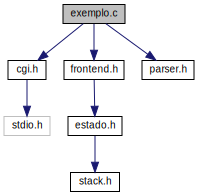
\includegraphics[width=270pt]{exemplo_8c__incl}
\end{center}
\end{figure}
\subsection*{Functions}
\begin{DoxyCompactItemize}
\item 
\hypertarget{exemplo_8c_ae66f6b31b5ad750f1fe042a706a4e3d4}{int \hyperlink{exemplo_8c_ae66f6b31b5ad750f1fe042a706a4e3d4}{main} ()}\label{exemplo_8c_ae66f6b31b5ad750f1fe042a706a4e3d4}

\begin{DoxyCompactList}\small\item\em Função que liga o jogo todo. \end{DoxyCompactList}\end{DoxyCompactItemize}


\subsection{Detailed Description}
Esqueleto do programa. 


\hypertarget{filemanager_8c}{\section{filemanager.\+c File Reference}
\label{filemanager_8c}\index{filemanager.\+c@{filemanager.\+c}}
}


Módulo de leitura de ficheiros.  


{\ttfamily \#include $<$stdlib.\+h$>$}\\*
{\ttfamily \#include $<$string.\+h$>$}\\*
{\ttfamily \#include \char`\"{}solver.\+h\char`\"{}}\\*
{\ttfamily \#include \char`\"{}filemanager.\+h\char`\"{}}\\*
{\ttfamily \#include \char`\"{}estado.\+h\char`\"{}}\\*
{\ttfamily \#include \char`\"{}cgi.\+h\char`\"{}}\\*
{\ttfamily \#include \char`\"{}frontend.\+h\char`\"{}}\\*
{\ttfamily \#include \char`\"{}state.\+h\char`\"{}}\\*
Include dependency graph for filemanager.\+c\+:
\nopagebreak
\begin{figure}[H]
\begin{center}
\leavevmode
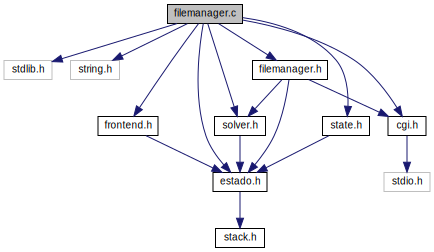
\includegraphics[width=350pt]{filemanager_8c__incl}
\end{center}
\end{figure}
\subsection*{Functions}
\begin{DoxyCompactItemize}
\item 
\hyperlink{estado_8c_afbffb4e9c242f93d5a2d607754ce2db8}{E\+S\+T\+A\+D\+O} \hyperlink{filemanager_8c_aa0525eadb0a7a8e368b3829ac5456a01}{select\+\_\+arcade} (char $\ast$path, int id)
\begin{DoxyCompactList}\small\item\em Seleciona um dos mapas disponibilizados pela aplicação. \end{DoxyCompactList}\item 
\hyperlink{estado_8c_afbffb4e9c242f93d5a2d607754ce2db8}{E\+S\+T\+A\+D\+O} \hyperlink{filemanager_8c_a1fc929d420e8048085000b6344fe2d78}{select\+\_\+padrao} (char $\ast$path, char $\ast$map, int $\ast$flag)
\begin{DoxyCompactList}\small\item\em Carrega um mapa selecionado pelo utilizador. \end{DoxyCompactList}\item 
\hyperlink{estado_8c_afbffb4e9c242f93d5a2d607754ce2db8}{E\+S\+T\+A\+D\+O} \hyperlink{filemanager_8c_ade9dcb29b01b24ea595ddc31ef56f5b4}{select\+\_\+random} (int id, int $\ast$flag)
\begin{DoxyCompactList}\small\item\em Função utilizada para ler um tabuleiro random. \end{DoxyCompactList}\item 
static \hyperlink{estado_8c_afbffb4e9c242f93d5a2d607754ce2db8}{E\+S\+T\+A\+D\+O} \hyperlink{filemanager_8c_aceda657a5528ae114fe6a12b24491f93}{ler\+\_\+puzzle\+\_\+padrao} (F\+I\+L\+E $\ast$file, int $\ast$flag)
\begin{DoxyCompactList}\small\item\em Esta função lê um puzzle na convenção dos docentes de li2. \end{DoxyCompactList}\item 
static char \hyperlink{filemanager_8c_a4011cb2274bbc7560c0e7875ae11a6e1}{convert\+Fl} (char ch, int $\ast$flag)
\begin{DoxyCompactList}\small\item\em Verifica a validade de uma determinada peça. \end{DoxyCompactList}\end{DoxyCompactItemize}


\subsection{Detailed Description}
Módulo de leitura de ficheiros. 



\subsection{Function Documentation}
\hypertarget{filemanager_8c_a4011cb2274bbc7560c0e7875ae11a6e1}{\index{filemanager.\+c@{filemanager.\+c}!convert\+Fl@{convert\+Fl}}
\index{convert\+Fl@{convert\+Fl}!filemanager.\+c@{filemanager.\+c}}
\subsubsection[{convert\+Fl}]{\setlength{\rightskip}{0pt plus 5cm}static char convert\+Fl (
\begin{DoxyParamCaption}
\item[{char}]{ch, }
\item[{int $\ast$}]{flag}
\end{DoxyParamCaption}
)\hspace{0.3cm}{\ttfamily [static]}}}\label{filemanager_8c_a4011cb2274bbc7560c0e7875ae11a6e1}


Verifica a validade de uma determinada peça. 


\begin{DoxyParams}{Parameters}
{\em ch} & Valor a comparar. \\
\hline
{\em flag} & Endereço onde irá ser colocado 1 se o caráter for válido, ou 0 caso contrário.\\
\hline
\end{DoxyParams}
\begin{DoxyReturn}{Returns}
Devolve o valor convertido caso seja válido, ou o próprio valor de comparação caso seja inválido. 
\end{DoxyReturn}
\hypertarget{filemanager_8c_aceda657a5528ae114fe6a12b24491f93}{\index{filemanager.\+c@{filemanager.\+c}!ler\+\_\+puzzle\+\_\+padrao@{ler\+\_\+puzzle\+\_\+padrao}}
\index{ler\+\_\+puzzle\+\_\+padrao@{ler\+\_\+puzzle\+\_\+padrao}!filemanager.\+c@{filemanager.\+c}}
\subsubsection[{ler\+\_\+puzzle\+\_\+padrao}]{\setlength{\rightskip}{0pt plus 5cm}static {\bf E\+S\+T\+A\+D\+O} ler\+\_\+puzzle\+\_\+padrao (
\begin{DoxyParamCaption}
\item[{F\+I\+L\+E $\ast$}]{file, }
\item[{int $\ast$}]{flag}
\end{DoxyParamCaption}
)\hspace{0.3cm}{\ttfamily [static]}}}\label{filemanager_8c_aceda657a5528ae114fe6a12b24491f93}


Esta função lê um puzzle na convenção dos docentes de li2. 


\begin{DoxyParams}{Parameters}
{\em file} & descritor de ficheiro F\+I\+L\+E já aberto. \\
\hline
{\em flag} & variavel com o endereço da variavel que registara o valor de sucesso ou insucceso desta função.\\
\hline
\end{DoxyParams}
\begin{DoxyReturn}{Returns}
Devolve o {\ttfamily E\+S\+T\+A\+D\+O} lido. 
\end{DoxyReturn}
\hypertarget{filemanager_8c_aa0525eadb0a7a8e368b3829ac5456a01}{\index{filemanager.\+c@{filemanager.\+c}!select\+\_\+arcade@{select\+\_\+arcade}}
\index{select\+\_\+arcade@{select\+\_\+arcade}!filemanager.\+c@{filemanager.\+c}}
\subsubsection[{select\+\_\+arcade}]{\setlength{\rightskip}{0pt plus 5cm}{\bf E\+S\+T\+A\+D\+O} select\+\_\+arcade (
\begin{DoxyParamCaption}
\item[{char $\ast$}]{path, }
\item[{int}]{id}
\end{DoxyParamCaption}
)}}\label{filemanager_8c_aa0525eadb0a7a8e368b3829ac5456a01}


Seleciona um dos mapas disponibilizados pela aplicação. 


\begin{DoxyParams}{Parameters}
{\em path} & Caminho interno onde estão guardados os mapas. \\
\hline
{\em id} & I\+D do mapa em questão.\\
\hline
\end{DoxyParams}
\begin{DoxyReturn}{Returns}
Devolve o {\ttfamily E\+S\+T\+A\+D\+O} selecionado. 
\end{DoxyReturn}
\hypertarget{filemanager_8c_a1fc929d420e8048085000b6344fe2d78}{\index{filemanager.\+c@{filemanager.\+c}!select\+\_\+padrao@{select\+\_\+padrao}}
\index{select\+\_\+padrao@{select\+\_\+padrao}!filemanager.\+c@{filemanager.\+c}}
\subsubsection[{select\+\_\+padrao}]{\setlength{\rightskip}{0pt plus 5cm}{\bf E\+S\+T\+A\+D\+O} select\+\_\+padrao (
\begin{DoxyParamCaption}
\item[{char $\ast$}]{path, }
\item[{char $\ast$}]{map, }
\item[{int $\ast$}]{flag}
\end{DoxyParamCaption}
)}}\label{filemanager_8c_a1fc929d420e8048085000b6344fe2d78}


Carrega um mapa selecionado pelo utilizador. 


\begin{DoxyParams}{Parameters}
{\em path} & Caminho do mapa que o utilizador pretende abrir. \\
\hline
{\em map} & Nome do ficheiro a carregar. \\
\hline
{\em flag} & Variavél com o endereço da variavél que registara o valor de sucesso ou insucceso desta função.\\
\hline
\end{DoxyParams}
\begin{DoxyReturn}{Returns}
Devolve o {\ttfamily E\+S\+T\+A\+D\+O} selecionado. 
\end{DoxyReturn}
\hypertarget{filemanager_8c_ade9dcb29b01b24ea595ddc31ef56f5b4}{\index{filemanager.\+c@{filemanager.\+c}!select\+\_\+random@{select\+\_\+random}}
\index{select\+\_\+random@{select\+\_\+random}!filemanager.\+c@{filemanager.\+c}}
\subsubsection[{select\+\_\+random}]{\setlength{\rightskip}{0pt plus 5cm}{\bf E\+S\+T\+A\+D\+O} select\+\_\+random (
\begin{DoxyParamCaption}
\item[{int}]{id, }
\item[{int $\ast$}]{flag}
\end{DoxyParamCaption}
)}}\label{filemanager_8c_ade9dcb29b01b24ea595ddc31ef56f5b4}


Função utilizada para ler um tabuleiro random. 


\begin{DoxyParams}{Parameters}
{\em id} & Id do ficheiro a carregar. \\
\hline
{\em flag} & Variavél onde se registará o valor de sucesso ou insucesso desta função.\\
\hline
\end{DoxyParams}
\begin{DoxyReturn}{Returns}
Estado lido. 
\end{DoxyReturn}

\hypertarget{filemanager_8h}{\section{filemanager.\+h File Reference}
\label{filemanager_8h}\index{filemanager.\+h@{filemanager.\+h}}
}


Módulo de leitura de ficheiros.  


{\ttfamily \#include \char`\"{}estado.\+h\char`\"{}}\\*
{\ttfamily \#include \char`\"{}solver.\+h\char`\"{}}\\*
{\ttfamily \#include \char`\"{}cgi.\+h\char`\"{}}\\*
Include dependency graph for filemanager.\+h\+:
\nopagebreak
\begin{figure}[H]
\begin{center}
\leavevmode
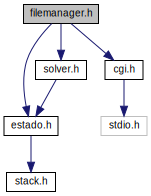
\includegraphics[width=223pt]{filemanager_8h__incl}
\end{center}
\end{figure}
This graph shows which files directly or indirectly include this file\+:
\nopagebreak
\begin{figure}[H]
\begin{center}
\leavevmode
\includegraphics[width=350pt]{filemanager_8h__dep__incl}
\end{center}
\end{figure}
\subsection*{Macros}
\begin{DoxyCompactItemize}
\item 
\#define \hyperlink{filemanager_8h_a65db46ec06db54c143d8c58f50a480af}{S\+E\+L\+E\+C\+T}(id)~\hyperlink{filemanager_8h_aa0525eadb0a7a8e368b3829ac5456a01}{select\+\_\+arcade}(\hyperlink{cgi_8h_af783caa0ab3eaa291b0af58fcb59d2b3}{F\+I\+L\+E\+\_\+\+P\+A\+T\+H}	,id)
\begin{DoxyCompactList}\small\item\em Macro para ler um mapa prédefinido. \end{DoxyCompactList}\item 
\#define \hyperlink{filemanager_8h_a312709802aca1cafd23ab379fb6fb9cc}{s\+Padrao}(map, flag)~(\hyperlink{filemanager_8h_a1fc929d420e8048085000b6344fe2d78}{select\+\_\+padrao}(\hyperlink{cgi_8h_a57f243883cb0b226e5af5ec6ceea763b}{M\+A\+P\+\_\+\+P\+A\+T\+H},map,\&(flag)))
\begin{DoxyCompactList}\small\item\em Macro para ler um mapa do utilizador. \end{DoxyCompactList}\end{DoxyCompactItemize}
\subsection*{Functions}
\begin{DoxyCompactItemize}
\item 
\hyperlink{estado_8c_afbffb4e9c242f93d5a2d607754ce2db8}{E\+S\+T\+A\+D\+O} \hyperlink{filemanager_8h_aa0525eadb0a7a8e368b3829ac5456a01}{select\+\_\+arcade} (char $\ast$path, int id)
\begin{DoxyCompactList}\small\item\em Seleciona um dos mapas disponibilizados pela aplicação. \end{DoxyCompactList}\item 
\hyperlink{estado_8c_afbffb4e9c242f93d5a2d607754ce2db8}{E\+S\+T\+A\+D\+O} \hyperlink{filemanager_8h_a1fc929d420e8048085000b6344fe2d78}{select\+\_\+padrao} (char $\ast$path, char $\ast$map, int $\ast$flag)
\begin{DoxyCompactList}\small\item\em Carrega um mapa selecionado pelo utilizador. \end{DoxyCompactList}\item 
\hyperlink{estado_8c_afbffb4e9c242f93d5a2d607754ce2db8}{E\+S\+T\+A\+D\+O} \hyperlink{filemanager_8h_ade9dcb29b01b24ea595ddc31ef56f5b4}{select\+\_\+random} (int id, int $\ast$flag)
\begin{DoxyCompactList}\small\item\em Função utilizada para ler um tabuleiro random. \end{DoxyCompactList}\end{DoxyCompactItemize}


\subsection{Detailed Description}
Módulo de leitura de ficheiros. 



\subsection{Macro Definition Documentation}
\hypertarget{filemanager_8h_a65db46ec06db54c143d8c58f50a480af}{\index{filemanager.\+h@{filemanager.\+h}!S\+E\+L\+E\+C\+T@{S\+E\+L\+E\+C\+T}}
\index{S\+E\+L\+E\+C\+T@{S\+E\+L\+E\+C\+T}!filemanager.\+h@{filemanager.\+h}}
\subsubsection[{S\+E\+L\+E\+C\+T}]{\setlength{\rightskip}{0pt plus 5cm}\#define S\+E\+L\+E\+C\+T(
\begin{DoxyParamCaption}
\item[{}]{id}
\end{DoxyParamCaption}
)~{\bf select\+\_\+arcade}({\bf F\+I\+L\+E\+\_\+\+P\+A\+T\+H}	,id)}}\label{filemanager_8h_a65db46ec06db54c143d8c58f50a480af}


Macro para ler um mapa prédefinido. 


\begin{DoxyParams}{Parameters}
{\em id} & número do mapa\\
\hline
\end{DoxyParams}
\begin{DoxyReturn}{Returns}
estado com o mapa lido 
\end{DoxyReturn}
\hypertarget{filemanager_8h_a312709802aca1cafd23ab379fb6fb9cc}{\index{filemanager.\+h@{filemanager.\+h}!s\+Padrao@{s\+Padrao}}
\index{s\+Padrao@{s\+Padrao}!filemanager.\+h@{filemanager.\+h}}
\subsubsection[{s\+Padrao}]{\setlength{\rightskip}{0pt plus 5cm}\#define s\+Padrao(
\begin{DoxyParamCaption}
\item[{}]{map, }
\item[{}]{flag}
\end{DoxyParamCaption}
)~({\bf select\+\_\+padrao}({\bf M\+A\+P\+\_\+\+P\+A\+T\+H},map,\&(flag)))}}\label{filemanager_8h_a312709802aca1cafd23ab379fb6fb9cc}


Macro para ler um mapa do utilizador. 


\begin{DoxyParams}{Parameters}
{\em map} & Nome do ficheiro a carregar. \\
\hline
{\em flag} & Variavél onde se registará o valor de sucesso ou insucesso desta função.\\
\hline
\end{DoxyParams}
\begin{DoxyReturn}{Returns}
estado com o mapa lido 
\end{DoxyReturn}


\subsection{Function Documentation}
\hypertarget{filemanager_8h_aa0525eadb0a7a8e368b3829ac5456a01}{\index{filemanager.\+h@{filemanager.\+h}!select\+\_\+arcade@{select\+\_\+arcade}}
\index{select\+\_\+arcade@{select\+\_\+arcade}!filemanager.\+h@{filemanager.\+h}}
\subsubsection[{select\+\_\+arcade}]{\setlength{\rightskip}{0pt plus 5cm}{\bf E\+S\+T\+A\+D\+O} select\+\_\+arcade (
\begin{DoxyParamCaption}
\item[{char $\ast$}]{path, }
\item[{int}]{id}
\end{DoxyParamCaption}
)}}\label{filemanager_8h_aa0525eadb0a7a8e368b3829ac5456a01}


Seleciona um dos mapas disponibilizados pela aplicação. 


\begin{DoxyParams}{Parameters}
{\em path} & Caminho interno onde estão guardados os mapas. \\
\hline
{\em id} & I\+D do mapa em questão.\\
\hline
\end{DoxyParams}
\begin{DoxyReturn}{Returns}
Devolve o {\ttfamily E\+S\+T\+A\+D\+O} selecionado. 
\end{DoxyReturn}
\hypertarget{filemanager_8h_a1fc929d420e8048085000b6344fe2d78}{\index{filemanager.\+h@{filemanager.\+h}!select\+\_\+padrao@{select\+\_\+padrao}}
\index{select\+\_\+padrao@{select\+\_\+padrao}!filemanager.\+h@{filemanager.\+h}}
\subsubsection[{select\+\_\+padrao}]{\setlength{\rightskip}{0pt plus 5cm}{\bf E\+S\+T\+A\+D\+O} select\+\_\+padrao (
\begin{DoxyParamCaption}
\item[{char $\ast$}]{path, }
\item[{char $\ast$}]{map, }
\item[{int $\ast$}]{flag}
\end{DoxyParamCaption}
)}}\label{filemanager_8h_a1fc929d420e8048085000b6344fe2d78}


Carrega um mapa selecionado pelo utilizador. 


\begin{DoxyParams}{Parameters}
{\em path} & Caminho do mapa que o utilizador pretende abrir. \\
\hline
{\em map} & Nome do ficheiro a carregar. \\
\hline
{\em flag} & Variavél com o endereço da variavél que registara o valor de sucesso ou insucceso desta função.\\
\hline
\end{DoxyParams}
\begin{DoxyReturn}{Returns}
Devolve o {\ttfamily E\+S\+T\+A\+D\+O} selecionado. 
\end{DoxyReturn}
\hypertarget{filemanager_8h_ade9dcb29b01b24ea595ddc31ef56f5b4}{\index{filemanager.\+h@{filemanager.\+h}!select\+\_\+random@{select\+\_\+random}}
\index{select\+\_\+random@{select\+\_\+random}!filemanager.\+h@{filemanager.\+h}}
\subsubsection[{select\+\_\+random}]{\setlength{\rightskip}{0pt plus 5cm}{\bf E\+S\+T\+A\+D\+O} select\+\_\+random (
\begin{DoxyParamCaption}
\item[{int}]{id, }
\item[{int $\ast$}]{flag}
\end{DoxyParamCaption}
)}}\label{filemanager_8h_ade9dcb29b01b24ea595ddc31ef56f5b4}


Função utilizada para ler um tabuleiro random. 


\begin{DoxyParams}{Parameters}
{\em id} & Id do ficheiro a carregar. \\
\hline
{\em flag} & Variavél onde se registará o valor de sucesso ou insucesso desta função.\\
\hline
\end{DoxyParams}
\begin{DoxyReturn}{Returns}
Estado lido. 
\end{DoxyReturn}

\hypertarget{frontend_8c}{\section{frontend.\+c File Reference}
\label{frontend_8c}\index{frontend.\+c@{frontend.\+c}}
}


Módulo de tratamento gráfico.  


{\ttfamily \#include \char`\"{}estado.\+h\char`\"{}}\\*
{\ttfamily \#include $<$stdlib.\+h$>$}\\*
{\ttfamily \#include $<$string.\+h$>$}\\*
{\ttfamily \#include \char`\"{}state.\+h\char`\"{}}\\*
{\ttfamily \#include \char`\"{}frontend.\+h\char`\"{}}\\*
{\ttfamily \#include \char`\"{}filemanager.\+h\char`\"{}}\\*
{\ttfamily \#include \char`\"{}decide.\+h\char`\"{}}\\*
{\ttfamily \#include \char`\"{}givehelp.\+h\char`\"{}}\\*
{\ttfamily \#include \char`\"{}solver.\+h\char`\"{}}\\*
{\ttfamily \#include \char`\"{}frontend\+Tab.\+h\char`\"{}}\\*
{\ttfamily \#include \char`\"{}leaderboard.\+h\char`\"{}}\\*
Include dependency graph for frontend.\+c\+:
\nopagebreak
\begin{figure}[H]
\begin{center}
\leavevmode
\includegraphics[width=350pt]{frontend_8c__incl}
\end{center}
\end{figure}
\subsection*{Macros}
\begin{DoxyCompactItemize}
\item 
\hypertarget{frontend_8c_a13475eb196c024c709557ec43810c63e}{\#define \hyperlink{frontend_8c_a13475eb196c024c709557ec43810c63e}{N\+M\+A\+P\+S}~7}\label{frontend_8c_a13475eb196c024c709557ec43810c63e}

\begin{DoxyCompactList}\small\item\em Constante que representa o número de mapas pré-\/definidos. \end{DoxyCompactList}\item 
\#define \hyperlink{frontend_8c_a4e7c62acc3de768680fb1ca1a7e4663a}{M\+A\+R\+G\+I\+N}(windowsize)~(windowsize/8)
\begin{DoxyCompactList}\small\item\em Macro para criar um valor de margem para trabalhar em frontend. \end{DoxyCompactList}\item 
\#define \hyperlink{frontend_8c_aabac370a28fbfb599c4dfcd65919e94d}{T\+E\+X\+T\+M\+A\+R\+G\+I\+N}(windowsize)~(windowsize/80)
\begin{DoxyCompactList}\small\item\em Macro para criar um valor de margem de texto para trabalhar em frontend. \end{DoxyCompactList}\item 
\#define \hyperlink{frontend_8c_a84857978d4c38e5397cc54ab849eaa3e}{S\+I\+Z\+E}(windowsize, x, d)~(d? (((windowsize$\ast$x)/16) + (windowsize/(16$\ast$d))) \+: ((windowsize$\ast$x)/16))
\begin{DoxyCompactList}\small\item\em Macro para criar um valor de tamanho para trabalhar em frontend. \end{DoxyCompactList}\end{DoxyCompactItemize}
\subsection*{Functions}
\begin{DoxyCompactItemize}
\item 
void \hyperlink{frontend_8c_a3bd06a6350b1adbcf2d2d71769b27ff9}{printstate} (\hyperlink{estado_8c_afbffb4e9c242f93d5a2d607754ce2db8}{E\+S\+T\+A\+D\+O} \hyperlink{structstate}{state}, int windowsize)
\begin{DoxyCompactList}\small\item\em Função que deesenha o Estado. \end{DoxyCompactList}\item 
void \hyperlink{frontend_8c_a24cc4ee047b57331edabed32f639b9f7}{select\+File} (char $\ast$name\+Tag, char $\ast$tag)
\begin{DoxyCompactList}\small\item\em Função que coloca uma textbox. \end{DoxyCompactList}\item 
static void \hyperlink{frontend_8c_afea3aedafac593a10ba6d2cf778a1612}{draw\+Menu\+Design\+Validate} (\hyperlink{estado_8c_afbffb4e9c242f93d5a2d607754ce2db8}{E\+S\+T\+A\+D\+O} \hyperlink{structstate}{state}, int windowsize)
\begin{DoxyCompactList}\small\item\em Função auxiliar para criar a validação do Menu desenhar tabuleiro. \end{DoxyCompactList}\item 
static void \hyperlink{frontend_8c_a4903992159a3ec4da981c1cc7418118d}{draw\+Menu\+Tab\+Design\+Stack} (\hyperlink{estado_8c_afbffb4e9c242f93d5a2d607754ce2db8}{E\+S\+T\+A\+D\+O} \hyperlink{structstate}{state}, int windowsize)
\begin{DoxyCompactList}\small\item\em Função auxiliar para criar o undo/redo do Menu desenhar tabuleiro. \end{DoxyCompactList}\item 
static void \hyperlink{frontend_8c_a0303eb77f758fd1bad7254b2beda86ed}{draw\+Menu\+Design\+Size} (\hyperlink{estado_8c_afbffb4e9c242f93d5a2d607754ce2db8}{E\+S\+T\+A\+D\+O} \hyperlink{structstate}{state}, int windowsize)
\begin{DoxyCompactList}\small\item\em Função auxiliar para criar o alterar tamanho do Menu desenhar tabuleiro. \end{DoxyCompactList}\item 
static void \hyperlink{frontend_8c_a05812a42c852508047f23de24c08d64a}{drawbuttonsplay\+Stack} (\hyperlink{estado_8c_afbffb4e9c242f93d5a2d607754ce2db8}{E\+S\+T\+A\+D\+O} \hyperlink{structstate}{state}, int windowsize)
\begin{DoxyCompactList}\small\item\em Função auxiliar para o Menu jogar Desenha undo/redo e ancoras. \end{DoxyCompactList}\item 
static void \hyperlink{frontend_8c_a2ecfaee0790d7c444e5ba53425b3dbca}{button\+Placer} (int x, int y, int size, char $\ast$link, char $\ast$pic)
\begin{DoxyCompactList}\small\item\em colocar um botão \end{DoxyCompactList}\item 
static void \hyperlink{frontend_8c_a748959ed642f1a42f3a84b0b33af40e7}{circulate\+Buttons} (\hyperlink{estado_8c_afbffb4e9c242f93d5a2d607754ce2db8}{E\+S\+T\+A\+D\+O} \hyperlink{structstate}{state}, int windowsize, int menu\+Prev, int menu\+Next)
\begin{DoxyCompactList}\small\item\em Função que desenha o rodapé do menu help. \end{DoxyCompactList}\item 
static void \hyperlink{frontend_8c_aaa606b9c4c0c87d167cbeebec3ab5308}{draw\+Menu\+Tab\+Design} (\hyperlink{estado_8c_afbffb4e9c242f93d5a2d607754ce2db8}{E\+S\+T\+A\+D\+O} \hyperlink{structstate}{state}, int windowsize)
\begin{DoxyCompactList}\small\item\em Função para criar o Menu desenhar tabuleiro. \end{DoxyCompactList}\item 
static void \hyperlink{frontend_8c_a487648a211fb66481701c83d119768e8}{drawbuttonsplay} (\hyperlink{estado_8c_afbffb4e9c242f93d5a2d607754ce2db8}{E\+S\+T\+A\+D\+O} \hyperlink{structstate}{state}, int windowsize)
\begin{DoxyCompactList}\small\item\em Função para o Menu jogar. \end{DoxyCompactList}\item 
static void \hyperlink{frontend_8c_a190791c8d661c12785cc74737f3265e2}{draw\+Pick\+Map} (\hyperlink{estado_8c_afbffb4e9c242f93d5a2d607754ce2db8}{E\+S\+T\+A\+D\+O} \hyperlink{structstate}{state}, int windowsize)
\begin{DoxyCompactList}\small\item\em Função que desenha o menu de escolher mapas. \end{DoxyCompactList}\item 
static void \hyperlink{frontend_8c_a845079297b8632ddf170fa54790490b7}{mode\+Select\+Menu} (\hyperlink{estado_8c_afbffb4e9c242f93d5a2d607754ce2db8}{E\+S\+T\+A\+D\+O} \hyperlink{structstate}{state}, int windowsize)
\begin{DoxyCompactList}\small\item\em Função que desenha o Menu para escolher o modo de jogo. \end{DoxyCompactList}\item 
static void \hyperlink{frontend_8c_a4e2fc98e7b289374d4f932a5a9515524}{draw\+Confirm\+Map} (\hyperlink{estado_8c_afbffb4e9c242f93d5a2d607754ce2db8}{E\+S\+T\+A\+D\+O} \hyperlink{structstate}{state}, int windowsize)
\begin{DoxyCompactList}\small\item\em Função que desenha o Menu para confirmar o mapa escolhido. \end{DoxyCompactList}\item 
static void \hyperlink{frontend_8c_a3e1bf9a4011354495add20600fd7fef3}{draw\+Menu\+Victory} (\hyperlink{estado_8c_afbffb4e9c242f93d5a2d607754ce2db8}{E\+S\+T\+A\+D\+O} \hyperlink{structstate}{state}, int windowsize)
\begin{DoxyCompactList}\small\item\em Função que desenha o Menu de Vitória. \end{DoxyCompactList}\item 
static void \hyperlink{frontend_8c_aff844c0da46af57d5cfba37d8b71bd96}{draw\+Menu\+Invalid\+Map} (\hyperlink{estado_8c_afbffb4e9c242f93d5a2d607754ce2db8}{E\+S\+T\+A\+D\+O} \hyperlink{structstate}{state}, int windowsize)
\begin{DoxyCompactList}\small\item\em Função que desenha o Menu de mapa inválido. \end{DoxyCompactList}\item 
static void \hyperlink{frontend_8c_a3485d524c07159e6bd35ecb39ad40780}{draw\+Menu\+Initial} (\hyperlink{estado_8c_afbffb4e9c242f93d5a2d607754ce2db8}{E\+S\+T\+A\+D\+O} \hyperlink{structstate}{state}, int windowsize)
\begin{DoxyCompactList}\small\item\em Função que desenha o Menu inicial. \end{DoxyCompactList}\item 
static void \hyperlink{frontend_8c_a9fe4e9db2a437f5a491e2540fca95bbc}{menu\+Random\+Map} (\hyperlink{estado_8c_afbffb4e9c242f93d5a2d607754ce2db8}{E\+S\+T\+A\+D\+O} \hyperlink{structstate}{state}, int windowsize)
\begin{DoxyCompactList}\small\item\em Função que desenha o Menu de mapas aleatórios. \end{DoxyCompactList}\item 
static void \hyperlink{frontend_8c_ab39bfd410378ea338fc2c75741883c4c}{menu\+Confirm\+R\+Map} (\hyperlink{estado_8c_afbffb4e9c242f93d5a2d607754ce2db8}{E\+S\+T\+A\+D\+O} \hyperlink{structstate}{state}, int windowsize)
\begin{DoxyCompactList}\small\item\em Função que desenha o Menu para cnfirmar mapas. \end{DoxyCompactList}\item 
static void \hyperlink{frontend_8c_acbbbd42e23dc3a761521bf6a81e5940b}{draw\+Hint} (\hyperlink{estado_8c_afbffb4e9c242f93d5a2d607754ce2db8}{E\+S\+T\+A\+D\+O} \hyperlink{structstate}{state}, int windowsize)
\begin{DoxyCompactList}\small\item\em Função auxiliar para o Menu jogar que desenha as hint. \end{DoxyCompactList}\item 
static void \hyperlink{frontend_8c_a24dd3bc3793c63c8b94164fd102bc439}{help\+P10} (\hyperlink{estado_8c_afbffb4e9c242f93d5a2d607754ce2db8}{E\+S\+T\+A\+D\+O} \hyperlink{structstate}{state}, int windowsize)
\begin{DoxyCompactList}\small\item\em Função que desenha o Menu de ajuda sobre leadearboard. \end{DoxyCompactList}\item 
static void \hyperlink{frontend_8c_ab1220950f1a95aa662a4f296e78699c0}{help\+P11} (\hyperlink{estado_8c_afbffb4e9c242f93d5a2d607754ce2db8}{E\+S\+T\+A\+D\+O} \hyperlink{structstate}{state}, int windowsize)
\begin{DoxyCompactList}\small\item\em Função que desenha o Menu de ajudas sobre jogar. \end{DoxyCompactList}\item 
static void \hyperlink{frontend_8c_a377305d3c60c5dc11c1c2cdd92ee4150}{help\+P12} (\hyperlink{estado_8c_afbffb4e9c242f93d5a2d607754ce2db8}{E\+S\+T\+A\+D\+O} \hyperlink{structstate}{state}, int windowsize)
\begin{DoxyCompactList}\small\item\em Função que desenha o Menu de ajudas sobre desenhar mapas. \end{DoxyCompactList}\item 
static void \hyperlink{frontend_8c_aca45f054ae44065acbcfabe1b44a0ec8}{help\+P13} (\hyperlink{estado_8c_afbffb4e9c242f93d5a2d607754ce2db8}{E\+S\+T\+A\+D\+O} \hyperlink{structstate}{state}, int windowsize)
\begin{DoxyCompactList}\small\item\em Função que desenha o Menu de ajudas sobre geração aleatória de mapas. \end{DoxyCompactList}\item 
static void \hyperlink{frontend_8c_a4702c27b0d07277af7f4d9e712152506}{help\+P14} (\hyperlink{estado_8c_afbffb4e9c242f93d5a2d607754ce2db8}{E\+S\+T\+A\+D\+O} \hyperlink{structstate}{state}, int windowsize)
\begin{DoxyCompactList}\small\item\em Função que desenha o Menu de ajudas sobre selecionar ficheiros. \end{DoxyCompactList}\item 
static void \hyperlink{frontend_8c_a8fbf9cd7d33b52b951eeaf21d9e9331e}{trofy\+Placer} (int windowsize, int N\+Leader)
\begin{DoxyCompactList}\small\item\em Função que desenha os trofeus no menu de leaderboard. \end{DoxyCompactList}\item 
static void \hyperlink{frontend_8c_ab8df0e7ab127c8814f8791d1f8656c15}{score\+Placer} (int windowsize, int N\+Leader, \hyperlink{leaderboard_8c_ae0cd0677a19c7077f6bba18c8276576e}{I\+N\+F\+O} v)
\begin{DoxyCompactList}\small\item\em Função que desenha os resultados no menu de leaderboard. \end{DoxyCompactList}\item 
static void \hyperlink{frontend_8c_af9ba7d1a7650c54f79a8590574ced887}{draw\+Menu\+Invalid\+Random} (\hyperlink{estado_8c_afbffb4e9c242f93d5a2d607754ce2db8}{E\+S\+T\+A\+D\+O} \hyperlink{structstate}{state}, int windowsize)
\begin{DoxyCompactList}\small\item\em Função que desenha o Menu de mapa inválido. \end{DoxyCompactList}\item 
static void \hyperlink{frontend_8c_a84d827d14d7b39c89702253e48dd8acb}{draw\+Leader\+Board} (\hyperlink{estado_8c_afbffb4e9c242f93d5a2d607754ce2db8}{E\+S\+T\+A\+D\+O} \hyperlink{structstate}{state}, int windowsize)
\begin{DoxyCompactList}\small\item\em Função que desenha o Menu de leaderboard. \end{DoxyCompactList}\end{DoxyCompactItemize}


\subsection{Detailed Description}
Módulo de tratamento gráfico. 



\subsection{Macro Definition Documentation}
\hypertarget{frontend_8c_a4e7c62acc3de768680fb1ca1a7e4663a}{\index{frontend.\+c@{frontend.\+c}!M\+A\+R\+G\+I\+N@{M\+A\+R\+G\+I\+N}}
\index{M\+A\+R\+G\+I\+N@{M\+A\+R\+G\+I\+N}!frontend.\+c@{frontend.\+c}}
\subsubsection[{M\+A\+R\+G\+I\+N}]{\setlength{\rightskip}{0pt plus 5cm}\#define M\+A\+R\+G\+I\+N(
\begin{DoxyParamCaption}
\item[{}]{windowsize}
\end{DoxyParamCaption}
)~(windowsize/8)}}\label{frontend_8c_a4e7c62acc3de768680fb1ca1a7e4663a}


Macro para criar um valor de margem para trabalhar em frontend. 


\begin{DoxyParams}{Parameters}
{\em windowsize} & a àrea disponível para desenhar\\
\hline
\end{DoxyParams}
\begin{DoxyReturn}{Returns}
valor de margem 
\end{DoxyReturn}
\hypertarget{frontend_8c_a84857978d4c38e5397cc54ab849eaa3e}{\index{frontend.\+c@{frontend.\+c}!S\+I\+Z\+E@{S\+I\+Z\+E}}
\index{S\+I\+Z\+E@{S\+I\+Z\+E}!frontend.\+c@{frontend.\+c}}
\subsubsection[{S\+I\+Z\+E}]{\setlength{\rightskip}{0pt plus 5cm}\#define S\+I\+Z\+E(
\begin{DoxyParamCaption}
\item[{}]{windowsize, }
\item[{}]{x, }
\item[{}]{d}
\end{DoxyParamCaption}
)~(d? (((windowsize$\ast$x)/16) + (windowsize/(16$\ast$d))) \+: ((windowsize$\ast$x)/16))}}\label{frontend_8c_a84857978d4c38e5397cc54ab849eaa3e}


Macro para criar um valor de tamanho para trabalhar em frontend. 


\begin{DoxyParams}{Parameters}
{\em windowsize} & a àrea disponível para desenhar \\
\hline
{\em x} & valor a multiplicar \\
\hline
{\em d} & valor a dividir\\
\hline
\end{DoxyParams}
\begin{DoxyReturn}{Returns}
valor de tamanho 
\end{DoxyReturn}
\hypertarget{frontend_8c_aabac370a28fbfb599c4dfcd65919e94d}{\index{frontend.\+c@{frontend.\+c}!T\+E\+X\+T\+M\+A\+R\+G\+I\+N@{T\+E\+X\+T\+M\+A\+R\+G\+I\+N}}
\index{T\+E\+X\+T\+M\+A\+R\+G\+I\+N@{T\+E\+X\+T\+M\+A\+R\+G\+I\+N}!frontend.\+c@{frontend.\+c}}
\subsubsection[{T\+E\+X\+T\+M\+A\+R\+G\+I\+N}]{\setlength{\rightskip}{0pt plus 5cm}\#define T\+E\+X\+T\+M\+A\+R\+G\+I\+N(
\begin{DoxyParamCaption}
\item[{}]{windowsize}
\end{DoxyParamCaption}
)~(windowsize/80)}}\label{frontend_8c_aabac370a28fbfb599c4dfcd65919e94d}


Macro para criar um valor de margem de texto para trabalhar em frontend. 


\begin{DoxyParams}{Parameters}
{\em windowsize} & a àrea disponível para desenhar\\
\hline
\end{DoxyParams}
\begin{DoxyReturn}{Returns}
valor de margem de texto 
\end{DoxyReturn}


\subsection{Function Documentation}
\hypertarget{frontend_8c_a2ecfaee0790d7c444e5ba53425b3dbca}{\index{frontend.\+c@{frontend.\+c}!button\+Placer@{button\+Placer}}
\index{button\+Placer@{button\+Placer}!frontend.\+c@{frontend.\+c}}
\subsubsection[{button\+Placer}]{\setlength{\rightskip}{0pt plus 5cm}static void button\+Placer (
\begin{DoxyParamCaption}
\item[{int}]{x, }
\item[{int}]{y, }
\item[{int}]{size, }
\item[{char $\ast$}]{link, }
\item[{char $\ast$}]{pic}
\end{DoxyParamCaption}
)\hspace{0.3cm}{\ttfamily [static]}}}\label{frontend_8c_a2ecfaee0790d7c444e5ba53425b3dbca}


colocar um botão 


\begin{DoxyParams}{Parameters}
{\em x} & offset do botão no eixo Ox \\
\hline
{\em y} & offset do botão no eixo Oy \\
\hline
{\em size} & A tamanho do botão \\
\hline
{\em link} & fim da hiperligação a colocar no botão \\
\hline
{\em pic} & nome da imagem do botão \\
\hline
\end{DoxyParams}
\hypertarget{frontend_8c_a748959ed642f1a42f3a84b0b33af40e7}{\index{frontend.\+c@{frontend.\+c}!circulate\+Buttons@{circulate\+Buttons}}
\index{circulate\+Buttons@{circulate\+Buttons}!frontend.\+c@{frontend.\+c}}
\subsubsection[{circulate\+Buttons}]{\setlength{\rightskip}{0pt plus 5cm}static void circulate\+Buttons (
\begin{DoxyParamCaption}
\item[{{\bf E\+S\+T\+A\+D\+O}}]{state, }
\item[{int}]{windowsize, }
\item[{int}]{menu\+Prev, }
\item[{int}]{menu\+Next}
\end{DoxyParamCaption}
)\hspace{0.3cm}{\ttfamily [static]}}}\label{frontend_8c_a748959ed642f1a42f3a84b0b33af40e7}


Função que desenha o rodapé do menu help. 


\begin{DoxyParams}{Parameters}
{\em state} & estado a desenhar \\
\hline
{\em windowsize} & tamanho da área disponível para desenhar \\
\hline
{\em menu\+Prev} & menu anterior \\
\hline
{\em menu\+Next} & menu seguinte \\
\hline
\end{DoxyParams}
\hypertarget{frontend_8c_a487648a211fb66481701c83d119768e8}{\index{frontend.\+c@{frontend.\+c}!drawbuttonsplay@{drawbuttonsplay}}
\index{drawbuttonsplay@{drawbuttonsplay}!frontend.\+c@{frontend.\+c}}
\subsubsection[{drawbuttonsplay}]{\setlength{\rightskip}{0pt plus 5cm}static void drawbuttonsplay (
\begin{DoxyParamCaption}
\item[{{\bf E\+S\+T\+A\+D\+O}}]{state, }
\item[{int}]{windowsize}
\end{DoxyParamCaption}
)\hspace{0.3cm}{\ttfamily [static]}}}\label{frontend_8c_a487648a211fb66481701c83d119768e8}


Função para o Menu jogar. 


\begin{DoxyParams}{Parameters}
{\em state} & o estado a desenhar \\
\hline
{\em windowsize} & tamanho da área disponível para desenhar \\
\hline
\end{DoxyParams}
\hypertarget{frontend_8c_a05812a42c852508047f23de24c08d64a}{\index{frontend.\+c@{frontend.\+c}!drawbuttonsplay\+Stack@{drawbuttonsplay\+Stack}}
\index{drawbuttonsplay\+Stack@{drawbuttonsplay\+Stack}!frontend.\+c@{frontend.\+c}}
\subsubsection[{drawbuttonsplay\+Stack}]{\setlength{\rightskip}{0pt plus 5cm}static void drawbuttonsplay\+Stack (
\begin{DoxyParamCaption}
\item[{{\bf E\+S\+T\+A\+D\+O}}]{state, }
\item[{int}]{windowsize}
\end{DoxyParamCaption}
)\hspace{0.3cm}{\ttfamily [static]}}}\label{frontend_8c_a05812a42c852508047f23de24c08d64a}


Função auxiliar para o Menu jogar Desenha undo/redo e ancoras. 


\begin{DoxyParams}{Parameters}
{\em state} & o estado a desenhar \\
\hline
{\em windowsize} & tamanho da área disponível para desenhar \\
\hline
\end{DoxyParams}
\hypertarget{frontend_8c_a4e2fc98e7b289374d4f932a5a9515524}{\index{frontend.\+c@{frontend.\+c}!draw\+Confirm\+Map@{draw\+Confirm\+Map}}
\index{draw\+Confirm\+Map@{draw\+Confirm\+Map}!frontend.\+c@{frontend.\+c}}
\subsubsection[{draw\+Confirm\+Map}]{\setlength{\rightskip}{0pt plus 5cm}static void draw\+Confirm\+Map (
\begin{DoxyParamCaption}
\item[{{\bf E\+S\+T\+A\+D\+O}}]{state, }
\item[{int}]{windowsize}
\end{DoxyParamCaption}
)\hspace{0.3cm}{\ttfamily [static]}}}\label{frontend_8c_a4e2fc98e7b289374d4f932a5a9515524}


Função que desenha o Menu para confirmar o mapa escolhido. 


\begin{DoxyParams}{Parameters}
{\em state} & o estado a desenhar \\
\hline
{\em windowsize} & tamanho da área disponível para desenhar \\
\hline
\end{DoxyParams}
\hypertarget{frontend_8c_acbbbd42e23dc3a761521bf6a81e5940b}{\index{frontend.\+c@{frontend.\+c}!draw\+Hint@{draw\+Hint}}
\index{draw\+Hint@{draw\+Hint}!frontend.\+c@{frontend.\+c}}
\subsubsection[{draw\+Hint}]{\setlength{\rightskip}{0pt plus 5cm}static void draw\+Hint (
\begin{DoxyParamCaption}
\item[{{\bf E\+S\+T\+A\+D\+O}}]{state, }
\item[{int}]{windowsize}
\end{DoxyParamCaption}
)\hspace{0.3cm}{\ttfamily [static]}}}\label{frontend_8c_acbbbd42e23dc3a761521bf6a81e5940b}


Função auxiliar para o Menu jogar que desenha as hint. 


\begin{DoxyParams}{Parameters}
{\em state} & o estado a desenhar \\
\hline
{\em windowsize} & tamanho da área disponível para desenhar \\
\hline
\end{DoxyParams}
\hypertarget{frontend_8c_a84d827d14d7b39c89702253e48dd8acb}{\index{frontend.\+c@{frontend.\+c}!draw\+Leader\+Board@{draw\+Leader\+Board}}
\index{draw\+Leader\+Board@{draw\+Leader\+Board}!frontend.\+c@{frontend.\+c}}
\subsubsection[{draw\+Leader\+Board}]{\setlength{\rightskip}{0pt plus 5cm}static void draw\+Leader\+Board (
\begin{DoxyParamCaption}
\item[{{\bf E\+S\+T\+A\+D\+O}}]{state, }
\item[{int}]{windowsize}
\end{DoxyParamCaption}
)\hspace{0.3cm}{\ttfamily [static]}}}\label{frontend_8c_a84d827d14d7b39c89702253e48dd8acb}


Função que desenha o Menu de leaderboard. 


\begin{DoxyParams}{Parameters}
{\em state} & o estado a desenhar \\
\hline
{\em windowsize} & tamanho da área disponível para desenhar \\
\hline
\end{DoxyParams}
\hypertarget{frontend_8c_a0303eb77f758fd1bad7254b2beda86ed}{\index{frontend.\+c@{frontend.\+c}!draw\+Menu\+Design\+Size@{draw\+Menu\+Design\+Size}}
\index{draw\+Menu\+Design\+Size@{draw\+Menu\+Design\+Size}!frontend.\+c@{frontend.\+c}}
\subsubsection[{draw\+Menu\+Design\+Size}]{\setlength{\rightskip}{0pt plus 5cm}static void draw\+Menu\+Design\+Size (
\begin{DoxyParamCaption}
\item[{{\bf E\+S\+T\+A\+D\+O}}]{state, }
\item[{int}]{windowsize}
\end{DoxyParamCaption}
)\hspace{0.3cm}{\ttfamily [static]}}}\label{frontend_8c_a0303eb77f758fd1bad7254b2beda86ed}


Função auxiliar para criar o alterar tamanho do Menu desenhar tabuleiro. 


\begin{DoxyParams}{Parameters}
{\em state} & o estado a desenhar \\
\hline
{\em windowsize} & tamanho da área disponível para desenhar \\
\hline
\end{DoxyParams}
\hypertarget{frontend_8c_afea3aedafac593a10ba6d2cf778a1612}{\index{frontend.\+c@{frontend.\+c}!draw\+Menu\+Design\+Validate@{draw\+Menu\+Design\+Validate}}
\index{draw\+Menu\+Design\+Validate@{draw\+Menu\+Design\+Validate}!frontend.\+c@{frontend.\+c}}
\subsubsection[{draw\+Menu\+Design\+Validate}]{\setlength{\rightskip}{0pt plus 5cm}static void draw\+Menu\+Design\+Validate (
\begin{DoxyParamCaption}
\item[{{\bf E\+S\+T\+A\+D\+O}}]{state, }
\item[{int}]{windowsize}
\end{DoxyParamCaption}
)\hspace{0.3cm}{\ttfamily [static]}}}\label{frontend_8c_afea3aedafac593a10ba6d2cf778a1612}


Função auxiliar para criar a validação do Menu desenhar tabuleiro. 


\begin{DoxyParams}{Parameters}
{\em state} & o estado a desenhar \\
\hline
{\em windowsize} & tamanho da área disponível para desenhar \\
\hline
\end{DoxyParams}
\hypertarget{frontend_8c_a3485d524c07159e6bd35ecb39ad40780}{\index{frontend.\+c@{frontend.\+c}!draw\+Menu\+Initial@{draw\+Menu\+Initial}}
\index{draw\+Menu\+Initial@{draw\+Menu\+Initial}!frontend.\+c@{frontend.\+c}}
\subsubsection[{draw\+Menu\+Initial}]{\setlength{\rightskip}{0pt plus 5cm}static void draw\+Menu\+Initial (
\begin{DoxyParamCaption}
\item[{{\bf E\+S\+T\+A\+D\+O}}]{state, }
\item[{int}]{windowsize}
\end{DoxyParamCaption}
)\hspace{0.3cm}{\ttfamily [static]}}}\label{frontend_8c_a3485d524c07159e6bd35ecb39ad40780}


Função que desenha o Menu inicial. 


\begin{DoxyParams}{Parameters}
{\em state} & o estado a desenhar \\
\hline
{\em windowsize} & tamanho da área disponível para desenhar \\
\hline
\end{DoxyParams}
\hypertarget{frontend_8c_aff844c0da46af57d5cfba37d8b71bd96}{\index{frontend.\+c@{frontend.\+c}!draw\+Menu\+Invalid\+Map@{draw\+Menu\+Invalid\+Map}}
\index{draw\+Menu\+Invalid\+Map@{draw\+Menu\+Invalid\+Map}!frontend.\+c@{frontend.\+c}}
\subsubsection[{draw\+Menu\+Invalid\+Map}]{\setlength{\rightskip}{0pt plus 5cm}static void draw\+Menu\+Invalid\+Map (
\begin{DoxyParamCaption}
\item[{{\bf E\+S\+T\+A\+D\+O}}]{state, }
\item[{int}]{windowsize}
\end{DoxyParamCaption}
)\hspace{0.3cm}{\ttfamily [static]}}}\label{frontend_8c_aff844c0da46af57d5cfba37d8b71bd96}


Função que desenha o Menu de mapa inválido. 


\begin{DoxyParams}{Parameters}
{\em state} & o estado a desenhar \\
\hline
{\em windowsize} & tamanho da área disponível para desenhar \\
\hline
\end{DoxyParams}
\hypertarget{frontend_8c_af9ba7d1a7650c54f79a8590574ced887}{\index{frontend.\+c@{frontend.\+c}!draw\+Menu\+Invalid\+Random@{draw\+Menu\+Invalid\+Random}}
\index{draw\+Menu\+Invalid\+Random@{draw\+Menu\+Invalid\+Random}!frontend.\+c@{frontend.\+c}}
\subsubsection[{draw\+Menu\+Invalid\+Random}]{\setlength{\rightskip}{0pt plus 5cm}static void draw\+Menu\+Invalid\+Random (
\begin{DoxyParamCaption}
\item[{{\bf E\+S\+T\+A\+D\+O}}]{state, }
\item[{int}]{windowsize}
\end{DoxyParamCaption}
)\hspace{0.3cm}{\ttfamily [static]}}}\label{frontend_8c_af9ba7d1a7650c54f79a8590574ced887}


Função que desenha o Menu de mapa inválido. 


\begin{DoxyParams}{Parameters}
{\em state} & o estado a desenhar \\
\hline
{\em windowsize} & tamanho da área disponível para desenhar \\
\hline
\end{DoxyParams}
\hypertarget{frontend_8c_aaa606b9c4c0c87d167cbeebec3ab5308}{\index{frontend.\+c@{frontend.\+c}!draw\+Menu\+Tab\+Design@{draw\+Menu\+Tab\+Design}}
\index{draw\+Menu\+Tab\+Design@{draw\+Menu\+Tab\+Design}!frontend.\+c@{frontend.\+c}}
\subsubsection[{draw\+Menu\+Tab\+Design}]{\setlength{\rightskip}{0pt plus 5cm}static void draw\+Menu\+Tab\+Design (
\begin{DoxyParamCaption}
\item[{{\bf E\+S\+T\+A\+D\+O}}]{state, }
\item[{int}]{windowsize}
\end{DoxyParamCaption}
)\hspace{0.3cm}{\ttfamily [static]}}}\label{frontend_8c_aaa606b9c4c0c87d167cbeebec3ab5308}


Função para criar o Menu desenhar tabuleiro. 


\begin{DoxyParams}{Parameters}
{\em state} & o estado a desenhar \\
\hline
{\em windowsize} & tamanho da área disponível para desenhar \\
\hline
\end{DoxyParams}
\hypertarget{frontend_8c_a4903992159a3ec4da981c1cc7418118d}{\index{frontend.\+c@{frontend.\+c}!draw\+Menu\+Tab\+Design\+Stack@{draw\+Menu\+Tab\+Design\+Stack}}
\index{draw\+Menu\+Tab\+Design\+Stack@{draw\+Menu\+Tab\+Design\+Stack}!frontend.\+c@{frontend.\+c}}
\subsubsection[{draw\+Menu\+Tab\+Design\+Stack}]{\setlength{\rightskip}{0pt plus 5cm}static void draw\+Menu\+Tab\+Design\+Stack (
\begin{DoxyParamCaption}
\item[{{\bf E\+S\+T\+A\+D\+O}}]{state, }
\item[{int}]{windowsize}
\end{DoxyParamCaption}
)\hspace{0.3cm}{\ttfamily [static]}}}\label{frontend_8c_a4903992159a3ec4da981c1cc7418118d}


Função auxiliar para criar o undo/redo do Menu desenhar tabuleiro. 


\begin{DoxyParams}{Parameters}
{\em state} & o estado a desenhar \\
\hline
{\em windowsize} & tamanho da área disponível para desenhar \\
\hline
\end{DoxyParams}
\hypertarget{frontend_8c_a3e1bf9a4011354495add20600fd7fef3}{\index{frontend.\+c@{frontend.\+c}!draw\+Menu\+Victory@{draw\+Menu\+Victory}}
\index{draw\+Menu\+Victory@{draw\+Menu\+Victory}!frontend.\+c@{frontend.\+c}}
\subsubsection[{draw\+Menu\+Victory}]{\setlength{\rightskip}{0pt plus 5cm}static void draw\+Menu\+Victory (
\begin{DoxyParamCaption}
\item[{{\bf E\+S\+T\+A\+D\+O}}]{state, }
\item[{int}]{windowsize}
\end{DoxyParamCaption}
)\hspace{0.3cm}{\ttfamily [static]}}}\label{frontend_8c_a3e1bf9a4011354495add20600fd7fef3}


Função que desenha o Menu de Vitória. 


\begin{DoxyParams}{Parameters}
{\em state} & o estado a desenhar \\
\hline
{\em windowsize} & tamanho da área disponível para desenhar \\
\hline
\end{DoxyParams}
\hypertarget{frontend_8c_a190791c8d661c12785cc74737f3265e2}{\index{frontend.\+c@{frontend.\+c}!draw\+Pick\+Map@{draw\+Pick\+Map}}
\index{draw\+Pick\+Map@{draw\+Pick\+Map}!frontend.\+c@{frontend.\+c}}
\subsubsection[{draw\+Pick\+Map}]{\setlength{\rightskip}{0pt plus 5cm}static void draw\+Pick\+Map (
\begin{DoxyParamCaption}
\item[{{\bf E\+S\+T\+A\+D\+O}}]{state, }
\item[{int}]{windowsize}
\end{DoxyParamCaption}
)\hspace{0.3cm}{\ttfamily [static]}}}\label{frontend_8c_a190791c8d661c12785cc74737f3265e2}


Função que desenha o menu de escolher mapas. 


\begin{DoxyParams}{Parameters}
{\em state} & o estado a desenhar \\
\hline
{\em windowsize} & tamanho da área disponível para desenhar \\
\hline
\end{DoxyParams}
\hypertarget{frontend_8c_a24dd3bc3793c63c8b94164fd102bc439}{\index{frontend.\+c@{frontend.\+c}!help\+P10@{help\+P10}}
\index{help\+P10@{help\+P10}!frontend.\+c@{frontend.\+c}}
\subsubsection[{help\+P10}]{\setlength{\rightskip}{0pt plus 5cm}static void help\+P10 (
\begin{DoxyParamCaption}
\item[{{\bf E\+S\+T\+A\+D\+O}}]{state, }
\item[{int}]{windowsize}
\end{DoxyParamCaption}
)\hspace{0.3cm}{\ttfamily [static]}}}\label{frontend_8c_a24dd3bc3793c63c8b94164fd102bc439}


Função que desenha o Menu de ajuda sobre leadearboard. 


\begin{DoxyParams}{Parameters}
{\em state} & o estado a desenhar \\
\hline
{\em windowsize} & tamanho da área disponível para desenhar \\
\hline
\end{DoxyParams}
\hypertarget{frontend_8c_ab1220950f1a95aa662a4f296e78699c0}{\index{frontend.\+c@{frontend.\+c}!help\+P11@{help\+P11}}
\index{help\+P11@{help\+P11}!frontend.\+c@{frontend.\+c}}
\subsubsection[{help\+P11}]{\setlength{\rightskip}{0pt plus 5cm}static void help\+P11 (
\begin{DoxyParamCaption}
\item[{{\bf E\+S\+T\+A\+D\+O}}]{state, }
\item[{int}]{windowsize}
\end{DoxyParamCaption}
)\hspace{0.3cm}{\ttfamily [static]}}}\label{frontend_8c_ab1220950f1a95aa662a4f296e78699c0}


Função que desenha o Menu de ajudas sobre jogar. 


\begin{DoxyParams}{Parameters}
{\em state} & o estado a desenhar \\
\hline
{\em windowsize} & tamanho da área disponível para desenhar \\
\hline
\end{DoxyParams}
\hypertarget{frontend_8c_a377305d3c60c5dc11c1c2cdd92ee4150}{\index{frontend.\+c@{frontend.\+c}!help\+P12@{help\+P12}}
\index{help\+P12@{help\+P12}!frontend.\+c@{frontend.\+c}}
\subsubsection[{help\+P12}]{\setlength{\rightskip}{0pt plus 5cm}static void help\+P12 (
\begin{DoxyParamCaption}
\item[{{\bf E\+S\+T\+A\+D\+O}}]{state, }
\item[{int}]{windowsize}
\end{DoxyParamCaption}
)\hspace{0.3cm}{\ttfamily [static]}}}\label{frontend_8c_a377305d3c60c5dc11c1c2cdd92ee4150}


Função que desenha o Menu de ajudas sobre desenhar mapas. 


\begin{DoxyParams}{Parameters}
{\em state} & o estado a desenhar \\
\hline
{\em windowsize} & tamanho da área disponível para desenhar \\
\hline
\end{DoxyParams}
\hypertarget{frontend_8c_aca45f054ae44065acbcfabe1b44a0ec8}{\index{frontend.\+c@{frontend.\+c}!help\+P13@{help\+P13}}
\index{help\+P13@{help\+P13}!frontend.\+c@{frontend.\+c}}
\subsubsection[{help\+P13}]{\setlength{\rightskip}{0pt plus 5cm}static void help\+P13 (
\begin{DoxyParamCaption}
\item[{{\bf E\+S\+T\+A\+D\+O}}]{state, }
\item[{int}]{windowsize}
\end{DoxyParamCaption}
)\hspace{0.3cm}{\ttfamily [static]}}}\label{frontend_8c_aca45f054ae44065acbcfabe1b44a0ec8}


Função que desenha o Menu de ajudas sobre geração aleatória de mapas. 


\begin{DoxyParams}{Parameters}
{\em state} & o estado a desenhar \\
\hline
{\em windowsize} & tamanho da área disponível para desenhar \\
\hline
\end{DoxyParams}
\hypertarget{frontend_8c_a4702c27b0d07277af7f4d9e712152506}{\index{frontend.\+c@{frontend.\+c}!help\+P14@{help\+P14}}
\index{help\+P14@{help\+P14}!frontend.\+c@{frontend.\+c}}
\subsubsection[{help\+P14}]{\setlength{\rightskip}{0pt plus 5cm}static void help\+P14 (
\begin{DoxyParamCaption}
\item[{{\bf E\+S\+T\+A\+D\+O}}]{state, }
\item[{int}]{windowsize}
\end{DoxyParamCaption}
)\hspace{0.3cm}{\ttfamily [static]}}}\label{frontend_8c_a4702c27b0d07277af7f4d9e712152506}


Função que desenha o Menu de ajudas sobre selecionar ficheiros. 


\begin{DoxyParams}{Parameters}
{\em state} & o estado a desenhar \\
\hline
{\em windowsize} & tamanho da área disponível para desenhar \\
\hline
\end{DoxyParams}
\hypertarget{frontend_8c_ab39bfd410378ea338fc2c75741883c4c}{\index{frontend.\+c@{frontend.\+c}!menu\+Confirm\+R\+Map@{menu\+Confirm\+R\+Map}}
\index{menu\+Confirm\+R\+Map@{menu\+Confirm\+R\+Map}!frontend.\+c@{frontend.\+c}}
\subsubsection[{menu\+Confirm\+R\+Map}]{\setlength{\rightskip}{0pt plus 5cm}static void menu\+Confirm\+R\+Map (
\begin{DoxyParamCaption}
\item[{{\bf E\+S\+T\+A\+D\+O}}]{state, }
\item[{int}]{windowsize}
\end{DoxyParamCaption}
)\hspace{0.3cm}{\ttfamily [static]}}}\label{frontend_8c_ab39bfd410378ea338fc2c75741883c4c}


Função que desenha o Menu para cnfirmar mapas. 


\begin{DoxyParams}{Parameters}
{\em state} & o estado a desenhar \\
\hline
{\em windowsize} & tamanho da área disponível para desenhar \\
\hline
\end{DoxyParams}
\hypertarget{frontend_8c_a9fe4e9db2a437f5a491e2540fca95bbc}{\index{frontend.\+c@{frontend.\+c}!menu\+Random\+Map@{menu\+Random\+Map}}
\index{menu\+Random\+Map@{menu\+Random\+Map}!frontend.\+c@{frontend.\+c}}
\subsubsection[{menu\+Random\+Map}]{\setlength{\rightskip}{0pt plus 5cm}static void menu\+Random\+Map (
\begin{DoxyParamCaption}
\item[{{\bf E\+S\+T\+A\+D\+O}}]{state, }
\item[{int}]{windowsize}
\end{DoxyParamCaption}
)\hspace{0.3cm}{\ttfamily [static]}}}\label{frontend_8c_a9fe4e9db2a437f5a491e2540fca95bbc}


Função que desenha o Menu de mapas aleatórios. 


\begin{DoxyParams}{Parameters}
{\em state} & o estado a desenhar \\
\hline
{\em windowsize} & tamanho da área disponível para desenhar \\
\hline
\end{DoxyParams}
\hypertarget{frontend_8c_a845079297b8632ddf170fa54790490b7}{\index{frontend.\+c@{frontend.\+c}!mode\+Select\+Menu@{mode\+Select\+Menu}}
\index{mode\+Select\+Menu@{mode\+Select\+Menu}!frontend.\+c@{frontend.\+c}}
\subsubsection[{mode\+Select\+Menu}]{\setlength{\rightskip}{0pt plus 5cm}static void mode\+Select\+Menu (
\begin{DoxyParamCaption}
\item[{{\bf E\+S\+T\+A\+D\+O}}]{state, }
\item[{int}]{windowsize}
\end{DoxyParamCaption}
)\hspace{0.3cm}{\ttfamily [static]}}}\label{frontend_8c_a845079297b8632ddf170fa54790490b7}


Função que desenha o Menu para escolher o modo de jogo. 


\begin{DoxyParams}{Parameters}
{\em state} & o estado a desenhar \\
\hline
{\em windowsize} & tamanho da área disponível para desenhar \\
\hline
\end{DoxyParams}
\hypertarget{frontend_8c_a3bd06a6350b1adbcf2d2d71769b27ff9}{\index{frontend.\+c@{frontend.\+c}!printstate@{printstate}}
\index{printstate@{printstate}!frontend.\+c@{frontend.\+c}}
\subsubsection[{printstate}]{\setlength{\rightskip}{0pt plus 5cm}void printstate (
\begin{DoxyParamCaption}
\item[{{\bf E\+S\+T\+A\+D\+O}}]{state, }
\item[{int}]{windowsize}
\end{DoxyParamCaption}
)}}\label{frontend_8c_a3bd06a6350b1adbcf2d2d71769b27ff9}


Função que deesenha o Estado. 


\begin{DoxyParams}{Parameters}
{\em state} & estado a desenhar \\
\hline
{\em windowsize} & tamanho da área disponível para desenhar \\
\hline
\end{DoxyParams}
\hypertarget{frontend_8c_ab8df0e7ab127c8814f8791d1f8656c15}{\index{frontend.\+c@{frontend.\+c}!score\+Placer@{score\+Placer}}
\index{score\+Placer@{score\+Placer}!frontend.\+c@{frontend.\+c}}
\subsubsection[{score\+Placer}]{\setlength{\rightskip}{0pt plus 5cm}static void score\+Placer (
\begin{DoxyParamCaption}
\item[{int}]{windowsize, }
\item[{int}]{N\+Leader, }
\item[{{\bf I\+N\+F\+O}}]{v}
\end{DoxyParamCaption}
)\hspace{0.3cm}{\ttfamily [static]}}}\label{frontend_8c_ab8df0e7ab127c8814f8791d1f8656c15}


Função que desenha os resultados no menu de leaderboard. 


\begin{DoxyParams}{Parameters}
{\em windowsize} & tamanho da área disponível para desenhar \\
\hline
{\em N\+Leader} & número de utilizadores a escrever \\
\hline
{\em v} & informação sobre a leaderboard \\
\hline
\end{DoxyParams}
\hypertarget{frontend_8c_a24cc4ee047b57331edabed32f639b9f7}{\index{frontend.\+c@{frontend.\+c}!select\+File@{select\+File}}
\index{select\+File@{select\+File}!frontend.\+c@{frontend.\+c}}
\subsubsection[{select\+File}]{\setlength{\rightskip}{0pt plus 5cm}void select\+File (
\begin{DoxyParamCaption}
\item[{char $\ast$}]{name\+Tag, }
\item[{char $\ast$}]{tag}
\end{DoxyParamCaption}
)}}\label{frontend_8c_a24cc4ee047b57331edabed32f639b9f7}


Função que coloca uma textbox. 


\begin{DoxyParams}{Parameters}
{\em name\+Tag} & nome da Text\+Box \\
\hline
{\em tag} & parte de trás da string \\
\hline
\end{DoxyParams}
\hypertarget{frontend_8c_a8fbf9cd7d33b52b951eeaf21d9e9331e}{\index{frontend.\+c@{frontend.\+c}!trofy\+Placer@{trofy\+Placer}}
\index{trofy\+Placer@{trofy\+Placer}!frontend.\+c@{frontend.\+c}}
\subsubsection[{trofy\+Placer}]{\setlength{\rightskip}{0pt plus 5cm}static void trofy\+Placer (
\begin{DoxyParamCaption}
\item[{int}]{windowsize, }
\item[{int}]{N\+Leader}
\end{DoxyParamCaption}
)\hspace{0.3cm}{\ttfamily [static]}}}\label{frontend_8c_a8fbf9cd7d33b52b951eeaf21d9e9331e}


Função que desenha os trofeus no menu de leaderboard. 


\begin{DoxyParams}{Parameters}
{\em windowsize} & tamanho da área disponível para desenhar \\
\hline
{\em N\+Leader} & número de utilizadores a escrever \\
\hline
\end{DoxyParams}

\hypertarget{frontend_8h}{\section{frontend.\+h File Reference}
\label{frontend_8h}\index{frontend.\+h@{frontend.\+h}}
}


Módulo de tratamento gráfico.  


{\ttfamily \#include \char`\"{}estado.\+h\char`\"{}}\\*
Include dependency graph for frontend.\+h\+:
\nopagebreak
\begin{figure}[H]
\begin{center}
\leavevmode
\includegraphics[width=138pt]{frontend_8h__incl}
\end{center}
\end{figure}
This graph shows which files directly or indirectly include this file\+:
\nopagebreak
\begin{figure}[H]
\begin{center}
\leavevmode
\includegraphics[width=350pt]{frontend_8h__dep__incl}
\end{center}
\end{figure}
\subsection*{Macros}
\begin{DoxyCompactItemize}
\item 
\hypertarget{frontend_8h_aa6bdf6a6d9916c343e1e17774d84a156}{\#define \hyperlink{frontend_8h_aa6bdf6a6d9916c343e1e17774d84a156}{B\+O\+D\+Y}~printf(\char`\"{}$<$body bgcolor='\#8\+F\+D8\+D8'$>$\textbackslash{}n\char`\"{})}\label{frontend_8h_aa6bdf6a6d9916c343e1e17774d84a156}

\begin{DoxyCompactList}\small\item\em Macro para abrir um body com a cor de fundo. \end{DoxyCompactList}\item 
\hypertarget{frontend_8h_a53dcc93404ee91f4f58e369c5cb28c3f}{\#define \hyperlink{frontend_8h_a53dcc93404ee91f4f58e369c5cb28c3f}{F\+E\+C\+H\+A\+R\+\_\+\+B\+O\+D\+Y}~printf(\char`\"{}$<$/body$>$\textbackslash{}n\char`\"{})}\label{frontend_8h_a53dcc93404ee91f4f58e369c5cb28c3f}

\begin{DoxyCompactList}\small\item\em Macro para fechar o body. \end{DoxyCompactList}\item 
\hypertarget{frontend_8h_a5f4e860a5a2d4a031933b102ab57a245}{\#define \hyperlink{frontend_8h_a5f4e860a5a2d4a031933b102ab57a245}{D\+I\+V\+\_\+\+C\+E\+N\+T\+R\+A\+R}~printf(\char`\"{}$<$div style='text-\/align\+:center;padding\+:50px'$>$\textbackslash{}n\char`\"{})}\label{frontend_8h_a5f4e860a5a2d4a031933b102ab57a245}

\begin{DoxyCompactList}\small\item\em Macro para cria o div que centra. \end{DoxyCompactList}\item 
\hypertarget{frontend_8h_a548edaa1e0b38a4a5e6662866a5836c3}{\#define \hyperlink{frontend_8h_a548edaa1e0b38a4a5e6662866a5836c3}{F\+E\+C\+H\+A\+R\+\_\+\+D\+I\+V}~printf(\char`\"{}$<$/div$>$\textbackslash{}n\char`\"{})}\label{frontend_8h_a548edaa1e0b38a4a5e6662866a5836c3}

\begin{DoxyCompactList}\small\item\em Macro para fechar div. \end{DoxyCompactList}\item 
\#define \hyperlink{frontend_8h_a1ba74891223a4e3dd6fe95ec633f965c}{calculate}(windowsize, win, mar, text)~(windowsize $\ast$ win + mar $\ast$ \hyperlink{frontend_8c_a4e7c62acc3de768680fb1ca1a7e4663a}{M\+A\+R\+G\+I\+N}(windowsize) + text $\ast$ \hyperlink{frontend_8c_aabac370a28fbfb599c4dfcd65919e94d}{T\+E\+X\+T\+M\+A\+R\+G\+I\+N}(windowsize))
\begin{DoxyCompactList}\small\item\em Macro para calcular o valor . \end{DoxyCompactList}\item 
\#define \hyperlink{frontend_8h_a35f1bfd38a7dbc1dbb3d45fa90d2e26f}{A\+C\+U\+\_\+\+I\+M\+A\+G\+E}(X, Y, E\+S\+C\+A\+L\+A, F\+I\+C\+H\+E\+I\+R\+O)
\begin{DoxyCompactList}\small\item\em Macro para criar uma imagem que ignora correções de escala. \end{DoxyCompactList}\end{DoxyCompactItemize}
\subsection*{Functions}
\begin{DoxyCompactItemize}
\item 
void \hyperlink{frontend_8h_a3bd06a6350b1adbcf2d2d71769b27ff9}{printstate} (\hyperlink{estado_8c_afbffb4e9c242f93d5a2d607754ce2db8}{E\+S\+T\+A\+D\+O} \hyperlink{structstate}{state}, int windowsize)
\begin{DoxyCompactList}\small\item\em Função que deesenha o Estado. \end{DoxyCompactList}\item 
void \hyperlink{frontend_8h_a24cc4ee047b57331edabed32f639b9f7}{select\+File} (char $\ast$name\+Tag, char $\ast$tag)
\begin{DoxyCompactList}\small\item\em Função que coloca uma textbox. \end{DoxyCompactList}\end{DoxyCompactItemize}


\subsection{Detailed Description}
Módulo de tratamento gráfico. 



\subsection{Macro Definition Documentation}
\hypertarget{frontend_8h_a35f1bfd38a7dbc1dbb3d45fa90d2e26f}{\index{frontend.\+h@{frontend.\+h}!A\+C\+U\+\_\+\+I\+M\+A\+G\+E@{A\+C\+U\+\_\+\+I\+M\+A\+G\+E}}
\index{A\+C\+U\+\_\+\+I\+M\+A\+G\+E@{A\+C\+U\+\_\+\+I\+M\+A\+G\+E}!frontend.\+h@{frontend.\+h}}
\subsubsection[{A\+C\+U\+\_\+\+I\+M\+A\+G\+E}]{\setlength{\rightskip}{0pt plus 5cm}\#define A\+C\+U\+\_\+\+I\+M\+A\+G\+E(
\begin{DoxyParamCaption}
\item[{}]{X, }
\item[{}]{Y, }
\item[{}]{E\+S\+C\+A\+L\+A, }
\item[{}]{F\+I\+C\+H\+E\+I\+R\+O}
\end{DoxyParamCaption}
)}}\label{frontend_8h_a35f1bfd38a7dbc1dbb3d45fa90d2e26f}
{\bfseries Value\+:}
\begin{DoxyCode}
printf(\textcolor{stringliteral}{"<image x=%d y=%d width=%d height=%d xlink:href=%s%s />\(\backslash\)n"}, \(\backslash\)
                                                 X, Y, ESCALA, ESCALA, 
      \hyperlink{cgi_8h_a6852d85bc96a09e605bbf4a2dcfc7a5c}{IMAGE\_PATH}, FICHEIRO)
\end{DoxyCode}


Macro para criar uma imagem que ignora correções de escala. 


\begin{DoxyParams}{Parameters}
{\em X} & A coordenada X do canto superior esquerdo. \\
\hline
{\em Y} & A coordenada Y do canto superior esquerdo. \\
\hline
{\em E\+S\+C\+A\+L\+A} & A escala da imagem. \\
\hline
{\em F\+I\+C\+H\+E\+I\+R\+O} & O caminho para o link do ficheiro. \\
\hline
\end{DoxyParams}
\hypertarget{frontend_8h_a1ba74891223a4e3dd6fe95ec633f965c}{\index{frontend.\+h@{frontend.\+h}!calculate@{calculate}}
\index{calculate@{calculate}!frontend.\+h@{frontend.\+h}}
\subsubsection[{calculate}]{\setlength{\rightskip}{0pt plus 5cm}\#define calculate(
\begin{DoxyParamCaption}
\item[{}]{windowsize, }
\item[{}]{win, }
\item[{}]{mar, }
\item[{}]{text}
\end{DoxyParamCaption}
)~(windowsize $\ast$ win + mar $\ast$ {\bf M\+A\+R\+G\+I\+N}(windowsize) + text $\ast$ {\bf T\+E\+X\+T\+M\+A\+R\+G\+I\+N}(windowsize))}}\label{frontend_8h_a1ba74891223a4e3dd6fe95ec633f965c}


Macro para calcular o valor . 


\begin{DoxyParams}{Parameters}
{\em windowsize} & tamanho da área disponível para desenhar. \\
\hline
{\em win} & multiplier pelo valor windowsize. \\
\hline
{\em mar} & multiplier pelo valor \hyperlink{frontend_8c_a4e7c62acc3de768680fb1ca1a7e4663a}{M\+A\+R\+G\+I\+N(windowsize)}. \\
\hline
{\em text} & multiplier pelo valor \hyperlink{frontend_8c_aabac370a28fbfb599c4dfcd65919e94d}{T\+E\+X\+T\+M\+A\+R\+G\+I\+N(windowsize)}. \\
\hline
\end{DoxyParams}


\subsection{Function Documentation}
\hypertarget{frontend_8h_a3bd06a6350b1adbcf2d2d71769b27ff9}{\index{frontend.\+h@{frontend.\+h}!printstate@{printstate}}
\index{printstate@{printstate}!frontend.\+h@{frontend.\+h}}
\subsubsection[{printstate}]{\setlength{\rightskip}{0pt plus 5cm}void printstate (
\begin{DoxyParamCaption}
\item[{{\bf E\+S\+T\+A\+D\+O}}]{state, }
\item[{int}]{windowsize}
\end{DoxyParamCaption}
)}}\label{frontend_8h_a3bd06a6350b1adbcf2d2d71769b27ff9}


Função que deesenha o Estado. 


\begin{DoxyParams}{Parameters}
{\em state} & estado a desenhar \\
\hline
{\em windowsize} & tamanho da área disponível para desenhar \\
\hline
\end{DoxyParams}
\hypertarget{frontend_8h_a24cc4ee047b57331edabed32f639b9f7}{\index{frontend.\+h@{frontend.\+h}!select\+File@{select\+File}}
\index{select\+File@{select\+File}!frontend.\+h@{frontend.\+h}}
\subsubsection[{select\+File}]{\setlength{\rightskip}{0pt plus 5cm}void select\+File (
\begin{DoxyParamCaption}
\item[{char $\ast$}]{name\+Tag, }
\item[{char $\ast$}]{tag}
\end{DoxyParamCaption}
)}}\label{frontend_8h_a24cc4ee047b57331edabed32f639b9f7}


Função que coloca uma textbox. 


\begin{DoxyParams}{Parameters}
{\em name\+Tag} & nome da Text\+Box \\
\hline
{\em tag} & parte de trás da string \\
\hline
\end{DoxyParams}

\hypertarget{frontendTab_8c}{\section{frontend\+Tab.\+c File Reference}
\label{frontendTab_8c}\index{frontend\+Tab.\+c@{frontend\+Tab.\+c}}
}


Módulo de tratamento gráfico, especializado ao tabuleiro.  


{\ttfamily \#include \char`\"{}estado.\+h\char`\"{}}\\*
{\ttfamily \#include $<$stdlib.\+h$>$}\\*
{\ttfamily \#include $<$string.\+h$>$}\\*
{\ttfamily \#include \char`\"{}state.\+h\char`\"{}}\\*
{\ttfamily \#include \char`\"{}frontend.\+h\char`\"{}}\\*
{\ttfamily \#include \char`\"{}filemanager.\+h\char`\"{}}\\*
{\ttfamily \#include \char`\"{}decide.\+h\char`\"{}}\\*
{\ttfamily \#include \char`\"{}givehelp.\+h\char`\"{}}\\*
{\ttfamily \#include \char`\"{}solver.\+h\char`\"{}}\\*
Include dependency graph for frontend\+Tab.\+c\+:
\nopagebreak
\begin{figure}[H]
\begin{center}
\leavevmode
\includegraphics[width=350pt]{frontendTab_8c__incl}
\end{center}
\end{figure}
\subsection*{Macros}
\begin{DoxyCompactItemize}
\item 
\#define \hyperlink{frontendTab_8c_aee7a7847a9a0c7a98bacd5e5fa09383c}{getmax}(n1, n2)~((n2)$>$(n1)) ? ((int)(n2))\+:((int)(n1))
\begin{DoxyCompactList}\small\item\em Macro que calcula o valor máximo entre dois valores. \end{DoxyCompactList}\end{DoxyCompactItemize}
\subsection*{Functions}
\begin{DoxyCompactItemize}
\item 
void \hyperlink{frontendTab_8c_aa931d57852fb164f2d99a6e339bc521b}{draw\+Tab} (\hyperlink{estado_8c_afbffb4e9c242f93d5a2d607754ce2db8}{E\+S\+T\+A\+D\+O} \hyperlink{structstate}{state}, int windowsize, int x, int y)
\begin{DoxyCompactList}\small\item\em Função que desenha o Tabuleiro. \end{DoxyCompactList}\item 
void \hyperlink{frontendTab_8c_a9d5ce8de0b474b3a08f544463433551a}{map\+Placer} (int x, int y, int size, int id, \hyperlink{estado_8c_afbffb4e9c242f93d5a2d607754ce2db8}{E\+S\+T\+A\+D\+O} \hyperlink{structstate}{state}, char $\ast$username)
\begin{DoxyCompactList}\small\item\em Função que desenha um Mapa clicavél dos mapas pré-\/definidos. \end{DoxyCompactList}\item 
static void \hyperlink{frontendTab_8c_a80ef7d7d4b66d2d915548f19c81cd690}{aidimage} (int x, int y, int size, char $\ast$img, char $\ast$buffer, int sign)
\begin{DoxyCompactList}\small\item\em Macro para criar colocar uma peça do tabuleiro. \end{DoxyCompactList}\item 
static void \hyperlink{frontendTab_8c_ad57282eb1359893bb2b389e7311a9d45}{putimage} (int ox, int oy, int x, int y, int size, int value, char $\ast$buffer, char menu, char linker)
\begin{DoxyCompactList}\small\item\em Macro para criar colocar uma peça do tabuleiro. \end{DoxyCompactList}\end{DoxyCompactItemize}


\subsection{Detailed Description}
Módulo de tratamento gráfico, especializado ao tabuleiro. 



\subsection{Macro Definition Documentation}
\hypertarget{frontendTab_8c_aee7a7847a9a0c7a98bacd5e5fa09383c}{\index{frontend\+Tab.\+c@{frontend\+Tab.\+c}!getmax@{getmax}}
\index{getmax@{getmax}!frontend\+Tab.\+c@{frontend\+Tab.\+c}}
\subsubsection[{getmax}]{\setlength{\rightskip}{0pt plus 5cm}\#define getmax(
\begin{DoxyParamCaption}
\item[{}]{n1, }
\item[{}]{n2}
\end{DoxyParamCaption}
)~((n2)$>$(n1)) ? ((int)(n2))\+:((int)(n1))}}\label{frontendTab_8c_aee7a7847a9a0c7a98bacd5e5fa09383c}


Macro que calcula o valor máximo entre dois valores. 


\begin{DoxyParams}{Parameters}
{\em n1} & valor a comparar \\
\hline
{\em n2} & valor a comparar\\
\hline
\end{DoxyParams}
\begin{DoxyReturn}{Returns}
o valor maior entre n1 e n2 
\end{DoxyReturn}


\subsection{Function Documentation}
\hypertarget{frontendTab_8c_a80ef7d7d4b66d2d915548f19c81cd690}{\index{frontend\+Tab.\+c@{frontend\+Tab.\+c}!aidimage@{aidimage}}
\index{aidimage@{aidimage}!frontend\+Tab.\+c@{frontend\+Tab.\+c}}
\subsubsection[{aidimage}]{\setlength{\rightskip}{0pt plus 5cm}static void aidimage (
\begin{DoxyParamCaption}
\item[{int}]{x, }
\item[{int}]{y, }
\item[{int}]{size, }
\item[{char $\ast$}]{img, }
\item[{char $\ast$}]{buffer, }
\item[{int}]{sign}
\end{DoxyParamCaption}
)\hspace{0.3cm}{\ttfamily [static]}}}\label{frontendTab_8c_a80ef7d7d4b66d2d915548f19c81cd690}


Macro para criar colocar uma peça do tabuleiro. 


\begin{DoxyParams}{Parameters}
{\em x} & abcissa do canto superior esquerdo da imagem \\
\hline
{\em y} & ordenada do canto superior esquerdo da imagem \\
\hline
{\em size} & tamanho da imagem \\
\hline
{\em img} & nome do ficheiro da imagem \\
\hline
{\em buffer} & hiperligação a colocar na imagem \\
\hline
{\em sign} & 0 para imprimir a imagem, 1 para imprimir e associar o link \\
\hline
\end{DoxyParams}
\hypertarget{frontendTab_8c_aa931d57852fb164f2d99a6e339bc521b}{\index{frontend\+Tab.\+c@{frontend\+Tab.\+c}!draw\+Tab@{draw\+Tab}}
\index{draw\+Tab@{draw\+Tab}!frontend\+Tab.\+c@{frontend\+Tab.\+c}}
\subsubsection[{draw\+Tab}]{\setlength{\rightskip}{0pt plus 5cm}void draw\+Tab (
\begin{DoxyParamCaption}
\item[{{\bf E\+S\+T\+A\+D\+O}}]{state, }
\item[{int}]{windowsize, }
\item[{int}]{x, }
\item[{int}]{y}
\end{DoxyParamCaption}
)}}\label{frontendTab_8c_aa931d57852fb164f2d99a6e339bc521b}


Função que desenha o Tabuleiro. 


\begin{DoxyParams}{Parameters}
{\em state} & estado a desenhar \\
\hline
{\em windowsize} & tamanho da área disponível para desenhar \\
\hline
{\em x} & offset do tabuleiro no eixo Ox \\
\hline
{\em y} & offset do tabuleiro no eixo Oy \\
\hline
\end{DoxyParams}
\hypertarget{frontendTab_8c_a9d5ce8de0b474b3a08f544463433551a}{\index{frontend\+Tab.\+c@{frontend\+Tab.\+c}!map\+Placer@{map\+Placer}}
\index{map\+Placer@{map\+Placer}!frontend\+Tab.\+c@{frontend\+Tab.\+c}}
\subsubsection[{map\+Placer}]{\setlength{\rightskip}{0pt plus 5cm}void map\+Placer (
\begin{DoxyParamCaption}
\item[{int}]{x, }
\item[{int}]{y, }
\item[{int}]{size, }
\item[{int}]{id, }
\item[{{\bf E\+S\+T\+A\+D\+O}}]{state, }
\item[{char $\ast$}]{username}
\end{DoxyParamCaption}
)}}\label{frontendTab_8c_a9d5ce8de0b474b3a08f544463433551a}


Função que desenha um Mapa clicavél dos mapas pré-\/definidos. 


\begin{DoxyParams}{Parameters}
{\em x} & abcissa do canto superior esquerdo do mapa \\
\hline
{\em y} & ordenada do canto superior esquerdo do mapa \\
\hline
{\em size} & tamanho do mapa \\
\hline
{\em id} & número do mapa que está a ser desenhado \\
\hline
{\em state} & o estado onde se encontra o mapa a desenhar \\
\hline
{\em username} & o nome do utilizador que está a jogar \\
\hline
\end{DoxyParams}
\hypertarget{frontendTab_8c_ad57282eb1359893bb2b389e7311a9d45}{\index{frontend\+Tab.\+c@{frontend\+Tab.\+c}!putimage@{putimage}}
\index{putimage@{putimage}!frontend\+Tab.\+c@{frontend\+Tab.\+c}}
\subsubsection[{putimage}]{\setlength{\rightskip}{0pt plus 5cm}static void putimage (
\begin{DoxyParamCaption}
\item[{int}]{ox, }
\item[{int}]{oy, }
\item[{int}]{x, }
\item[{int}]{y, }
\item[{int}]{size, }
\item[{int}]{value, }
\item[{char $\ast$}]{buffer, }
\item[{char}]{menu, }
\item[{char}]{linker}
\end{DoxyParamCaption}
)\hspace{0.3cm}{\ttfamily [static]}}}\label{frontendTab_8c_ad57282eb1359893bb2b389e7311a9d45}


Macro para criar colocar uma peça do tabuleiro. 


\begin{DoxyParams}{Parameters}
{\em ox} & offset da peça no eixo Ox \\
\hline
{\em oy} & offset da peça no eixo Oy \\
\hline
{\em x} & número da linha da peça \\
\hline
{\em y} & número da coluna da peça \\
\hline
{\em size} & tamanho da peça \\
\hline
{\em value} & descrição enum da peça \\
\hline
{\em buffer} & hiperligação a colocar na peça \\
\hline
{\em menu} & menu onde se encontra o tabuleiro \\
\hline
{\em linker} & identificação para desenhar soltos com link \\
\hline
\end{DoxyParams}

\hypertarget{frontendTab_8h}{\section{frontend\+Tab.\+h File Reference}
\label{frontendTab_8h}\index{frontend\+Tab.\+h@{frontend\+Tab.\+h}}
}


Módulo de tratamento gráfico, especializado ao tabuleiro.  


This graph shows which files directly or indirectly include this file\+:
\nopagebreak
\begin{figure}[H]
\begin{center}
\leavevmode
\includegraphics[width=156pt]{frontendTab_8h__dep__incl}
\end{center}
\end{figure}
\subsection*{Functions}
\begin{DoxyCompactItemize}
\item 
void \hyperlink{frontendTab_8h_aa931d57852fb164f2d99a6e339bc521b}{draw\+Tab} (\hyperlink{estado_8c_afbffb4e9c242f93d5a2d607754ce2db8}{E\+S\+T\+A\+D\+O} \hyperlink{structstate}{state}, int windowsize, int x, int y)
\begin{DoxyCompactList}\small\item\em Função que desenha o Tabuleiro. \end{DoxyCompactList}\item 
void \hyperlink{frontendTab_8h_a9d5ce8de0b474b3a08f544463433551a}{map\+Placer} (int x, int y, int size, int id, \hyperlink{estado_8c_afbffb4e9c242f93d5a2d607754ce2db8}{E\+S\+T\+A\+D\+O} \hyperlink{structstate}{state}, char $\ast$username)
\begin{DoxyCompactList}\small\item\em Função que desenha um Mapa clicavél dos mapas pré-\/definidos. \end{DoxyCompactList}\end{DoxyCompactItemize}


\subsection{Detailed Description}
Módulo de tratamento gráfico, especializado ao tabuleiro. 



\subsection{Function Documentation}
\hypertarget{frontendTab_8h_aa931d57852fb164f2d99a6e339bc521b}{\index{frontend\+Tab.\+h@{frontend\+Tab.\+h}!draw\+Tab@{draw\+Tab}}
\index{draw\+Tab@{draw\+Tab}!frontend\+Tab.\+h@{frontend\+Tab.\+h}}
\subsubsection[{draw\+Tab}]{\setlength{\rightskip}{0pt plus 5cm}void draw\+Tab (
\begin{DoxyParamCaption}
\item[{{\bf E\+S\+T\+A\+D\+O}}]{state, }
\item[{int}]{windowsize, }
\item[{int}]{x, }
\item[{int}]{y}
\end{DoxyParamCaption}
)}}\label{frontendTab_8h_aa931d57852fb164f2d99a6e339bc521b}


Função que desenha o Tabuleiro. 


\begin{DoxyParams}{Parameters}
{\em state} & estado a desenhar \\
\hline
{\em windowsize} & tamanho da área disponível para desenhar \\
\hline
{\em x} & offset do tabuleiro no eixo Ox \\
\hline
{\em y} & offset do tabuleiro no eixo Oy \\
\hline
\end{DoxyParams}
\hypertarget{frontendTab_8h_a9d5ce8de0b474b3a08f544463433551a}{\index{frontend\+Tab.\+h@{frontend\+Tab.\+h}!map\+Placer@{map\+Placer}}
\index{map\+Placer@{map\+Placer}!frontend\+Tab.\+h@{frontend\+Tab.\+h}}
\subsubsection[{map\+Placer}]{\setlength{\rightskip}{0pt plus 5cm}void map\+Placer (
\begin{DoxyParamCaption}
\item[{int}]{x, }
\item[{int}]{y, }
\item[{int}]{size, }
\item[{int}]{id, }
\item[{{\bf E\+S\+T\+A\+D\+O}}]{state, }
\item[{char $\ast$}]{username}
\end{DoxyParamCaption}
)}}\label{frontendTab_8h_a9d5ce8de0b474b3a08f544463433551a}


Função que desenha um Mapa clicavél dos mapas pré-\/definidos. 


\begin{DoxyParams}{Parameters}
{\em x} & abcissa do canto superior esquerdo do mapa \\
\hline
{\em y} & ordenada do canto superior esquerdo do mapa \\
\hline
{\em size} & tamanho do mapa \\
\hline
{\em id} & número do mapa que está a ser desenhado \\
\hline
{\em state} & o estado onde se encontra o mapa a desenhar \\
\hline
{\em username} & o nome do utilizador que está a jogar \\
\hline
\end{DoxyParams}

\hypertarget{gerar_8c}{\section{gerar.\+c File Reference}
\label{gerar_8c}\index{gerar.\+c@{gerar.\+c}}
}


Ficheiro de geração de tabuleiro aleatório.  


{\ttfamily \#include $<$time.\+h$>$}\\*
{\ttfamily \#include \char`\"{}solver.\+h\char`\"{}}\\*
{\ttfamily \#include $<$stdio.\+h$>$}\\*
{\ttfamily \#include $<$stdlib.\+h$>$}\\*
Include dependency graph for gerar.\+c\+:
\nopagebreak
\begin{figure}[H]
\begin{center}
\leavevmode
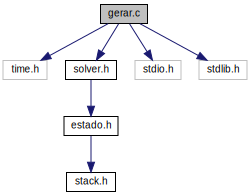
\includegraphics[width=323pt]{gerar_8c__incl}
\end{center}
\end{figure}
\subsection*{Macros}
\begin{DoxyCompactItemize}
\item 
\#define \hyperlink{gerar_8c_a62436901460e715d963d209b0dbba8cb}{lim}(num)~((num$>$0) \&\& (num $<$= \hyperlink{estado_8h_ab02e1c5c6948bf8cf3c21a0acad8a578}{M\+A\+X\+\_\+\+G\+R\+I\+D}))
\begin{DoxyCompactList}\small\item\em Macro destinada a definir o limite de dimensões. \end{DoxyCompactList}\end{DoxyCompactItemize}
\subsection*{Functions}
\begin{DoxyCompactItemize}
\item 
\hypertarget{gerar_8c_a0ddf1224851353fc92bfbff6f499fa97}{int \hyperlink{gerar_8c_a0ddf1224851353fc92bfbff6f499fa97}{main} (int argc, char $\ast$argv\mbox{[}$\,$\mbox{]})}\label{gerar_8c_a0ddf1224851353fc92bfbff6f499fa97}

\begin{DoxyCompactList}\small\item\em Função main para gerar mapas random. \end{DoxyCompactList}\end{DoxyCompactItemize}


\subsection{Detailed Description}
Ficheiro de geração de tabuleiro aleatório. 



\subsection{Macro Definition Documentation}
\hypertarget{gerar_8c_a62436901460e715d963d209b0dbba8cb}{\index{gerar.\+c@{gerar.\+c}!lim@{lim}}
\index{lim@{lim}!gerar.\+c@{gerar.\+c}}
\subsubsection[{lim}]{\setlength{\rightskip}{0pt plus 5cm}\#define lim(
\begin{DoxyParamCaption}
\item[{}]{num}
\end{DoxyParamCaption}
)~((num$>$0) \&\& (num $<$= {\bf M\+A\+X\+\_\+\+G\+R\+I\+D}))}}\label{gerar_8c_a62436901460e715d963d209b0dbba8cb}


Macro destinada a definir o limite de dimensões. 


\begin{DoxyParams}{Parameters}
{\em num} & Valor a comparar. \\
\hline
\end{DoxyParams}

\hypertarget{givehelp_8c}{\section{givehelp.\+c File Reference}
\label{givehelp_8c}\index{givehelp.\+c@{givehelp.\+c}}
}


Módulo para fornecimento de ajudas.  


{\ttfamily \#include \char`\"{}estado.\+h\char`\"{}}\\*
{\ttfamily \#include \char`\"{}decide.\+h\char`\"{}}\\*
{\ttfamily \#include \char`\"{}givehelp.\+h\char`\"{}}\\*
{\ttfamily \#include \char`\"{}validate.\+h\char`\"{}}\\*
{\ttfamily \#include \char`\"{}solver.\+h\char`\"{}}\\*
{\ttfamily \#include $<$stdio.\+h$>$}\\*
{\ttfamily \#include $<$string.\+h$>$}\\*
Include dependency graph for givehelp.\+c\+:
\nopagebreak
\begin{figure}[H]
\begin{center}
\leavevmode
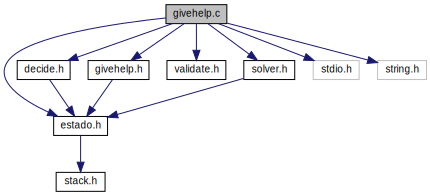
\includegraphics[width=350pt]{givehelp_8c__incl}
\end{center}
\end{figure}
\subsection*{Macros}
\begin{DoxyCompactItemize}
\item 
\#define \hyperlink{givehelp_8c_a337cd8a8e5c0d38e251d972e9533fa50}{is\+\_\+solto}(num)~((num == S\+O\+L\+\_\+\+X) $\vert$$\vert$ (num == S\+O\+L\+\_\+\+O) $\vert$$\vert$ (num == V\+A\+Z\+I\+A))
\begin{DoxyCompactList}\small\item\em verifica se uma peca é S\+O\+L ou V\+A\+Z\+I\+A \end{DoxyCompactList}\end{DoxyCompactItemize}
\subsection*{Functions}
\begin{DoxyCompactItemize}
\item 
int \hyperlink{givehelp_8c_a76ebe592c1a541633c7e5662fff4eb8e}{possiblepath} (\hyperlink{estado_8c_afbffb4e9c242f93d5a2d607754ce2db8}{E\+S\+T\+A\+D\+O} \hyperlink{structstate}{state}, int i, int j)
\begin{DoxyCompactList}\small\item\em Indica o número de casas válidas que uma posição consegue percorrer. \end{DoxyCompactList}\item 
void \hyperlink{givehelp_8c_a56fc46f28368685f0897f3f58f80b039}{givehelp} (\hyperlink{estado_8c_afbffb4e9c242f93d5a2d607754ce2db8}{E\+S\+T\+A\+D\+O} e)
\begin{DoxyCompactList}\small\item\em Função que altera o Estado e dá ajudas. \end{DoxyCompactList}\item 
static int \hyperlink{givehelp_8c_a7ef25cc065d026571f0a09c6f37a3dc0}{putnatural} (\hyperlink{estado_8c_afbffb4e9c242f93d5a2d607754ce2db8}{E\+S\+T\+A\+D\+O} src, \hyperlink{estado_8c_afbffb4e9c242f93d5a2d607754ce2db8}{E\+S\+T\+A\+D\+O} comp)
\begin{DoxyCompactList}\small\item\em Função que dá ajudas naturais Se existirem duas pecas em linha ela coloca uma peça válida numa das extremidades. \end{DoxyCompactList}\item 
static int \hyperlink{givehelp_8c_a040597e0574505bd0f83f904df3debed}{searchcomp} (\hyperlink{estado_8c_afbffb4e9c242f93d5a2d607754ce2db8}{E\+S\+T\+A\+D\+O} src, \hyperlink{estado_8c_afbffb4e9c242f93d5a2d607754ce2db8}{E\+S\+T\+A\+D\+O} comp, int indc)
\begin{DoxyCompactList}\small\item\em Faz um procura complementária entre dois estados diferentes. \end{DoxyCompactList}\end{DoxyCompactItemize}


\subsection{Detailed Description}
Módulo para fornecimento de ajudas. 



\subsection{Macro Definition Documentation}
\hypertarget{givehelp_8c_a337cd8a8e5c0d38e251d972e9533fa50}{\index{givehelp.\+c@{givehelp.\+c}!is\+\_\+solto@{is\+\_\+solto}}
\index{is\+\_\+solto@{is\+\_\+solto}!givehelp.\+c@{givehelp.\+c}}
\subsubsection[{is\+\_\+solto}]{\setlength{\rightskip}{0pt plus 5cm}\#define is\+\_\+solto(
\begin{DoxyParamCaption}
\item[{}]{num}
\end{DoxyParamCaption}
)~((num == S\+O\+L\+\_\+\+X) $\vert$$\vert$ (num == S\+O\+L\+\_\+\+O) $\vert$$\vert$ (num == V\+A\+Z\+I\+A))}}\label{givehelp_8c_a337cd8a8e5c0d38e251d972e9533fa50}


verifica se uma peca é S\+O\+L ou V\+A\+Z\+I\+A 


\begin{DoxyParams}{Parameters}
{\em num} & valor\\
\hline
\end{DoxyParams}
\begin{DoxyReturn}{Returns}
1 se for S\+O\+L ou V\+A\+Z\+I\+A, 0 caso contrário 
\end{DoxyReturn}


\subsection{Function Documentation}
\hypertarget{givehelp_8c_a56fc46f28368685f0897f3f58f80b039}{\index{givehelp.\+c@{givehelp.\+c}!givehelp@{givehelp}}
\index{givehelp@{givehelp}!givehelp.\+c@{givehelp.\+c}}
\subsubsection[{givehelp}]{\setlength{\rightskip}{0pt plus 5cm}void givehelp (
\begin{DoxyParamCaption}
\item[{{\bf E\+S\+T\+A\+D\+O}}]{e}
\end{DoxyParamCaption}
)}}\label{givehelp_8c_a56fc46f28368685f0897f3f58f80b039}


Função que altera o Estado e dá ajudas. 

A função inicialmente verifica se o número de ajudas disponivél é maior que 0, se o for, então é criada uma solução de {\ttfamily state} , sendo então utilizada a função {\ttfamily putnatural} , de forma a encontrar peças sem verificar a solução. Se {\ttfamily putnatural} não encontrar nenhuma ajuda então é utilizada a função {\ttfamily searchcomp} com {\ttfamily indc} a {\bfseries 0} de forma a que não utilize recursividade. Se não encontrar nenhum elemento a alterar desta forma então corre a função {\ttfamily searchcomp} com {\ttfamily indc} a {\bfseries 1} , então será utilizada recursividade e mais de uma peça será alterada.


\begin{DoxyParams}{Parameters}
{\em e} & Estado a alterar.\\
\hline
\end{DoxyParams}
\begin{DoxySeeAlso}{See also}
\hyperlink{estado_8h_ab3e47d845be6ab389f1cb63532ab9313}{get\+E\+\_\+help} 

\hyperlink{solver_8h_a6102730d9741f071f2354149756162a6}{solve} 

\hyperlink{givehelp_8c_a7ef25cc065d026571f0a09c6f37a3dc0}{putnatural} 

\hyperlink{givehelp_8c_a040597e0574505bd0f83f904df3debed}{searchcomp} 
\end{DoxySeeAlso}
\hypertarget{givehelp_8c_a76ebe592c1a541633c7e5662fff4eb8e}{\index{givehelp.\+c@{givehelp.\+c}!possiblepath@{possiblepath}}
\index{possiblepath@{possiblepath}!givehelp.\+c@{givehelp.\+c}}
\subsubsection[{possiblepath}]{\setlength{\rightskip}{0pt plus 5cm}int possiblepath (
\begin{DoxyParamCaption}
\item[{{\bf E\+S\+T\+A\+D\+O}}]{state, }
\item[{int}]{i, }
\item[{int}]{j}
\end{DoxyParamCaption}
)}}\label{givehelp_8c_a76ebe592c1a541633c7e5662fff4eb8e}


Indica o número de casas válidas que uma posição consegue percorrer. 

Verifica a grelha de um estado, e consoante as peças à volta de uma posição, percorre as possibilidades de peças até alcançar {\bfseries S\+O\+L\+\_\+\+O} indicando quantas destas peças intermédias são válidas.


\begin{DoxyParams}{Parameters}
{\em state} & Estado que se pretende alterar. \\
\hline
{\em i} & Linha que se pretende verificar. \\
\hline
{\em j} & Coluna que se pretende verificar.\\
\hline
\end{DoxyParams}
\begin{DoxyReturn}{Returns}
O número de peças que são válidas.
\end{DoxyReturn}
\begin{DoxySeeAlso}{See also}
\hyperlink{validate_8h_a7cc26aa61c34f0e7fd569e7e176ef8e4}{valtab} 
\end{DoxySeeAlso}
\hypertarget{givehelp_8c_a7ef25cc065d026571f0a09c6f37a3dc0}{\index{givehelp.\+c@{givehelp.\+c}!putnatural@{putnatural}}
\index{putnatural@{putnatural}!givehelp.\+c@{givehelp.\+c}}
\subsubsection[{putnatural}]{\setlength{\rightskip}{0pt plus 5cm}static int putnatural (
\begin{DoxyParamCaption}
\item[{{\bf E\+S\+T\+A\+D\+O}}]{src, }
\item[{{\bf E\+S\+T\+A\+D\+O}}]{comp}
\end{DoxyParamCaption}
)\hspace{0.3cm}{\ttfamily [static]}}}\label{givehelp_8c_a7ef25cc065d026571f0a09c6f37a3dc0}


Função que dá ajudas naturais Se existirem duas pecas em linha ela coloca uma peça válida numa das extremidades. 


\begin{DoxyParams}{Parameters}
{\em src} & estado onde se encontra o mapa a procurar \\
\hline
{\em comp} & local onde são armazenadas as alterações\\
\hline
\end{DoxyParams}
\begin{DoxyReturn}{Returns}
1 se conseguir encontrar pecas nessa condição, 0 se não encontrar
\end{DoxyReturn}
\begin{DoxySeeAlso}{See also}
\hyperlink{givehelp_8c_a76ebe592c1a541633c7e5662fff4eb8e}{possiblepath} 

\hyperlink{decide_8h_ac47faeda9e29e07135095e3711035845}{playadvance} 

\hyperlink{decide_8h_ae13669ac08e09c81d021c5569733e0fb}{formove} 

\hyperlink{stack_8h_a734636978e69eedc1efd53ddc858d360}{push} 

\hyperlink{estado_8h_aa61011eadf880d552d197316ad4b30bb}{get\+E\+\_\+stack} 
\end{DoxySeeAlso}
\hypertarget{givehelp_8c_a040597e0574505bd0f83f904df3debed}{\index{givehelp.\+c@{givehelp.\+c}!searchcomp@{searchcomp}}
\index{searchcomp@{searchcomp}!givehelp.\+c@{givehelp.\+c}}
\subsubsection[{searchcomp}]{\setlength{\rightskip}{0pt plus 5cm}static int searchcomp (
\begin{DoxyParamCaption}
\item[{{\bf E\+S\+T\+A\+D\+O}}]{src, }
\item[{{\bf E\+S\+T\+A\+D\+O}}]{comp, }
\item[{int}]{indc}
\end{DoxyParamCaption}
)\hspace{0.3cm}{\ttfamily [static]}}}\label{givehelp_8c_a040597e0574505bd0f83f904df3debed}


Faz um procura complementária entre dois estados diferentes. 

A função percorre ambos os estados, sendo que {\ttfamily comp} deve corresponder à solução do estado {\ttfamily src}. A cada posição que corresponda a uma peça do tipo {\bfseries S\+O\+L\+T\+O} ou {\bfseries V\+A\+Z\+I\+A} verifica que está é igual à peça que se encontra na mesma posição na solução, caso sejam iguais as peças nenhuma operação é efetuada. Caso contrário, o elemento em questão é alterada para a peça correspondente na solução. O que gera três casos\+:


\begin{DoxyItemize}
\item A nova peça é válida, então o elemento é alterado, e colocado na {\bfseries S\+T\+A\+C\+K} .
\item A nova peça é inválida e {\ttfamily indc} é {\bfseries 0} , então a peça será alterada para o elemento antigo que lá se encontrava.
\item A nova peça é inválida e {\ttfamily indc} é diferente de {\bfseries 0} , então é utilizada recursividade de forma a alterar um número arbitrário de peças até que o tabuleiro se torne válido.
\end{DoxyItemize}
\begin{DoxyParams}{Parameters}
{\em src} & O estado que irá ser alterado. \\
\hline
{\em comp} & O estado que servirá de base de alteração. \\
\hline
{\em indc} & 0 se não se pretender utilizar recursividade, diferente de {\bfseries 0} caso contrário.\\
\hline
\end{DoxyParams}
\begin{DoxyReturn}{Returns}
0 se encontrou uma peça para alterar, 1 caso contrário.
\end{DoxyReturn}
\begin{DoxySeeAlso}{See also}
\hyperlink{givehelp_8c_a337cd8a8e5c0d38e251d972e9533fa50}{is\+\_\+solto} 

\hyperlink{stack_8h_a734636978e69eedc1efd53ddc858d360}{push} 

\hyperlink{estado_8h_aa61011eadf880d552d197316ad4b30bb}{get\+E\+\_\+stack} 
\end{DoxySeeAlso}

\hypertarget{givehelp_8h}{\section{givehelp.\+h File Reference}
\label{givehelp_8h}\index{givehelp.\+h@{givehelp.\+h}}
}


Módulo para fornecimento de ajudas.  


{\ttfamily \#include \char`\"{}estado.\+h\char`\"{}}\\*
Include dependency graph for givehelp.\+h\+:
\nopagebreak
\begin{figure}[H]
\begin{center}
\leavevmode
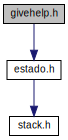
\includegraphics[width=140pt]{givehelp_8h__incl}
\end{center}
\end{figure}
This graph shows which files directly or indirectly include this file\+:
\nopagebreak
\begin{figure}[H]
\begin{center}
\leavevmode
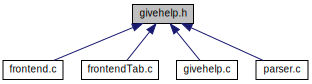
\includegraphics[width=350pt]{givehelp_8h__dep__incl}
\end{center}
\end{figure}
\subsection*{Functions}
\begin{DoxyCompactItemize}
\item 
int \hyperlink{givehelp_8h_a76ebe592c1a541633c7e5662fff4eb8e}{possiblepath} (\hyperlink{estado_8c_afbffb4e9c242f93d5a2d607754ce2db8}{E\+S\+T\+A\+D\+O} \hyperlink{structstate}{state}, int i, int j)
\begin{DoxyCompactList}\small\item\em Indica o número de casas válidas que uma posição consegue percorrer. \end{DoxyCompactList}\item 
void \hyperlink{givehelp_8h_a56fc46f28368685f0897f3f58f80b039}{givehelp} (\hyperlink{estado_8c_afbffb4e9c242f93d5a2d607754ce2db8}{E\+S\+T\+A\+D\+O} e)
\begin{DoxyCompactList}\small\item\em Função que altera o Estado e dá ajudas. \end{DoxyCompactList}\end{DoxyCompactItemize}


\subsection{Detailed Description}
Módulo para fornecimento de ajudas. 



\subsection{Function Documentation}
\hypertarget{givehelp_8h_a56fc46f28368685f0897f3f58f80b039}{\index{givehelp.\+h@{givehelp.\+h}!givehelp@{givehelp}}
\index{givehelp@{givehelp}!givehelp.\+h@{givehelp.\+h}}
\subsubsection[{givehelp}]{\setlength{\rightskip}{0pt plus 5cm}void givehelp (
\begin{DoxyParamCaption}
\item[{{\bf E\+S\+T\+A\+D\+O}}]{e}
\end{DoxyParamCaption}
)}}\label{givehelp_8h_a56fc46f28368685f0897f3f58f80b039}


Função que altera o Estado e dá ajudas. 

A função inicialmente verifica se o número de ajudas disponivél é maior que 0, se o for, então é criada uma solução de {\ttfamily state} , sendo então utilizada a função {\ttfamily putnatural} , de forma a encontrar peças sem verificar a solução. Se {\ttfamily putnatural} não encontrar nenhuma ajuda então é utilizada a função {\ttfamily searchcomp} com {\ttfamily indc} a {\bfseries 0} de forma a que não utilize recursividade. Se não encontrar nenhum elemento a alterar desta forma então corre a função {\ttfamily searchcomp} com {\ttfamily indc} a {\bfseries 1} , então será utilizada recursividade e mais de uma peça será alterada.


\begin{DoxyParams}{Parameters}
{\em e} & Estado a alterar.\\
\hline
\end{DoxyParams}
\begin{DoxySeeAlso}{See also}
\hyperlink{estado_8h_ab3e47d845be6ab389f1cb63532ab9313}{get\+E\+\_\+help} 

\hyperlink{solver_8h_a6102730d9741f071f2354149756162a6}{solve} 

\hyperlink{givehelp_8c_a7ef25cc065d026571f0a09c6f37a3dc0}{putnatural} 

\hyperlink{givehelp_8c_a040597e0574505bd0f83f904df3debed}{searchcomp} 
\end{DoxySeeAlso}
\hypertarget{givehelp_8h_a76ebe592c1a541633c7e5662fff4eb8e}{\index{givehelp.\+h@{givehelp.\+h}!possiblepath@{possiblepath}}
\index{possiblepath@{possiblepath}!givehelp.\+h@{givehelp.\+h}}
\subsubsection[{possiblepath}]{\setlength{\rightskip}{0pt plus 5cm}int possiblepath (
\begin{DoxyParamCaption}
\item[{{\bf E\+S\+T\+A\+D\+O}}]{state, }
\item[{int}]{i, }
\item[{int}]{j}
\end{DoxyParamCaption}
)}}\label{givehelp_8h_a76ebe592c1a541633c7e5662fff4eb8e}


Indica o número de casas válidas que uma posição consegue percorrer. 

Verifica a grelha de um estado, e consoante as peças à volta de uma posição, percorre as possibilidades de peças até alcançar {\bfseries S\+O\+L\+\_\+\+O} indicando quantas destas peças intermédias são válidas.


\begin{DoxyParams}{Parameters}
{\em state} & Estado que se pretende alterar. \\
\hline
{\em i} & Linha que se pretende verificar. \\
\hline
{\em j} & Coluna que se pretende verificar.\\
\hline
\end{DoxyParams}
\begin{DoxyReturn}{Returns}
O número de peças que são válidas.
\end{DoxyReturn}
\begin{DoxySeeAlso}{See also}
\hyperlink{validate_8h_a7cc26aa61c34f0e7fd569e7e176ef8e4}{valtab} 
\end{DoxySeeAlso}

\hypertarget{leaderboard_8c}{\section{leaderboard.\+c File Reference}
\label{leaderboard_8c}\index{leaderboard.\+c@{leaderboard.\+c}}
}


Módulo de obtenção da leaderboard.  


{\ttfamily \#include $<$stdlib.\+h$>$}\\*
{\ttfamily \#include $<$stdio.\+h$>$}\\*
{\ttfamily \#include $<$string.\+h$>$}\\*
{\ttfamily \#include \char`\"{}leaderboard.\+h\char`\"{}}\\*
Include dependency graph for leaderboard.\+c\+:
\nopagebreak
\begin{figure}[H]
\begin{center}
\leavevmode
\includegraphics[width=350pt]{leaderboard_8c__incl}
\end{center}
\end{figure}
\subsection*{Classes}
\begin{DoxyCompactItemize}
\item 
struct \hyperlink{structinfo}{info}
\begin{DoxyCompactList}\small\item\em Estrutura onde é guardada a informação usada pela leaderboard. \end{DoxyCompactList}\end{DoxyCompactItemize}
\subsection*{Macros}
\begin{DoxyCompactItemize}
\item 
\hypertarget{leaderboard_8c_a9b18aaa9c44ed30a23fcf8811d4c2763}{\#define \hyperlink{leaderboard_8c_a9b18aaa9c44ed30a23fcf8811d4c2763}{D\+I\+R\+I\+N\+F\+O}~\char`\"{}/usr/local/games/Ganda\+Galo/users/users.\+save\char`\"{}}\label{leaderboard_8c_a9b18aaa9c44ed30a23fcf8811d4c2763}

\begin{DoxyCompactList}\small\item\em Diretória onde se encontra o ficheiro onde são guardados todos os utilizadores. \end{DoxyCompactList}\end{DoxyCompactItemize}
\subsection*{Typedefs}
\begin{DoxyCompactItemize}
\item 
\hypertarget{leaderboard_8c_ae0cd0677a19c7077f6bba18c8276576e}{typedef struct \hyperlink{structinfo}{info} $\ast$ \hyperlink{leaderboard_8c_ae0cd0677a19c7077f6bba18c8276576e}{I\+N\+F\+O}}\label{leaderboard_8c_ae0cd0677a19c7077f6bba18c8276576e}

\begin{DoxyCompactList}\small\item\em Estrutura onde é guardada a informação usada pela leaderboard. \end{DoxyCompactList}\end{DoxyCompactItemize}
\subsection*{Functions}
\begin{DoxyCompactItemize}
\item 
char $\ast$ \hyperlink{leaderboard_8c_a71a5dab891243597dbb138612ecf3857}{get\+Info\+\_\+user} (\hyperlink{leaderboard_8c_ae0cd0677a19c7077f6bba18c8276576e}{I\+N\+F\+O} v, int i)
\begin{DoxyCompactList}\small\item\em Função que obtêm o utilizador associado a um bloco de informação. \end{DoxyCompactList}\item 
int \hyperlink{leaderboard_8c_a3596e9737c2017c08210285adbf50541}{get\+Info\+\_\+wins} (\hyperlink{leaderboard_8c_ae0cd0677a19c7077f6bba18c8276576e}{I\+N\+F\+O} v, int i)
\begin{DoxyCompactList}\small\item\em Função que obtêm o número de vitórias associado a um bloco de informação. \end{DoxyCompactList}\item 
int \hyperlink{leaderboard_8c_a6b7ea262cb48cc841d5ba76db2984768}{get\+\_\+info} (\hyperlink{leaderboard_8c_ae0cd0677a19c7077f6bba18c8276576e}{I\+N\+F\+O} $\ast$v, int N)
\begin{DoxyCompactList}\small\item\em Função que indica um array de {\ttfamily I\+N\+F\+O} contendo a leaderboard. \end{DoxyCompactList}\item 
void \hyperlink{leaderboard_8c_aa23db304e56c4f0e17bb06e619fe6956}{push\+\_\+info} (char $\ast$user, int wins)
\begin{DoxyCompactList}\small\item\em Função que adiciona nova informação ao ficheiro. Consoante o utilizador e o número de vitória coloca no ficheiro {\ttfamily D\+I\+R\+I\+N\+F\+O} a informação passada como argumento. Da seguinte forma\+: \end{DoxyCompactList}\item 
static void \hyperlink{leaderboard_8c_ada70e23e1c8bd904bd090ff8f9d03966}{make\+\_\+info} ()
\begin{DoxyCompactList}\small\item\em Função que verifica a existência de {\ttfamily D\+I\+R\+I\+N\+F\+O} . Caso o ficheiro não exista, então é criado. \end{DoxyCompactList}\item 
static int \hyperlink{leaderboard_8c_ae790da7f1eee2be78a2e51c248ee4282}{size\+\_\+info} ()
\begin{DoxyCompactList}\small\item\em Função que devolve o número de elementos no ficheiro {\ttfamily D\+I\+R\+I\+N\+F\+O} . \end{DoxyCompactList}\item 
static \hyperlink{leaderboard_8c_ae0cd0677a19c7077f6bba18c8276576e}{I\+N\+F\+O} \hyperlink{leaderboard_8c_a57f19b982e416216fe5865738c7e5b2a}{list\+\_\+info} (int $\ast$x)
\begin{DoxyCompactList}\small\item\em Cria um array com todos os elementos do ficheiro. \end{DoxyCompactList}\item 
static int \hyperlink{leaderboard_8c_a03c0eeffe08be732225b326846f7a107}{cmp\+\_\+info} (const void $\ast$a, const void $\ast$b)
\begin{DoxyCompactList}\small\item\em Função de comparação utilizada no sorting. \end{DoxyCompactList}\item 
static void \hyperlink{leaderboard_8c_a31d353bb4c3a5c08b568d5b5a4e98696}{sort\+\_\+info} (\hyperlink{leaderboard_8c_ae0cd0677a19c7077f6bba18c8276576e}{I\+N\+F\+O} v)
\begin{DoxyCompactList}\small\item\em Efetua o sorting do array de {\ttfamily I\+N\+F\+O} . \end{DoxyCompactList}\end{DoxyCompactItemize}


\subsection{Detailed Description}
Módulo de obtenção da leaderboard. 



\subsection{Function Documentation}
\hypertarget{leaderboard_8c_a03c0eeffe08be732225b326846f7a107}{\index{leaderboard.\+c@{leaderboard.\+c}!cmp\+\_\+info@{cmp\+\_\+info}}
\index{cmp\+\_\+info@{cmp\+\_\+info}!leaderboard.\+c@{leaderboard.\+c}}
\subsubsection[{cmp\+\_\+info}]{\setlength{\rightskip}{0pt plus 5cm}static int cmp\+\_\+info (
\begin{DoxyParamCaption}
\item[{const void $\ast$}]{a, }
\item[{const void $\ast$}]{b}
\end{DoxyParamCaption}
)\hspace{0.3cm}{\ttfamily [static]}}}\label{leaderboard_8c_a03c0eeffe08be732225b326846f7a107}


Função de comparação utilizada no sorting. 


\begin{DoxyParams}{Parameters}
{\em a} & Primeiro valor a comparar. \\
\hline
{\em b} & Segundo valor a confirmar.\\
\hline
\end{DoxyParams}
\begin{DoxyReturn}{Returns}
O valor da comparação. 
\end{DoxyReturn}
\hypertarget{leaderboard_8c_a6b7ea262cb48cc841d5ba76db2984768}{\index{leaderboard.\+c@{leaderboard.\+c}!get\+\_\+info@{get\+\_\+info}}
\index{get\+\_\+info@{get\+\_\+info}!leaderboard.\+c@{leaderboard.\+c}}
\subsubsection[{get\+\_\+info}]{\setlength{\rightskip}{0pt plus 5cm}int get\+\_\+info (
\begin{DoxyParamCaption}
\item[{{\bf I\+N\+F\+O} $\ast$}]{v, }
\item[{int}]{N}
\end{DoxyParamCaption}
)}}\label{leaderboard_8c_a6b7ea262cb48cc841d5ba76db2984768}


Função que indica um array de {\ttfamily I\+N\+F\+O} contendo a leaderboard. 


\begin{DoxyParams}{Parameters}
{\em v} & Apontador para o endereço onde irá ser colocada a leaderboard. \\
\hline
{\em N} & Número máximo de elementos colocados.\\
\hline
\end{DoxyParams}
\begin{DoxyReturn}{Returns}
Números de elementos colocados.
\end{DoxyReturn}
\begin{DoxySeeAlso}{See also}
\hyperlink{leaderboard_8c_a57f19b982e416216fe5865738c7e5b2a}{list\+\_\+info} 

\hyperlink{leaderboard_8c_a31d353bb4c3a5c08b568d5b5a4e98696}{sort\+\_\+info} 

\hyperlink{leaderboard_8c_ae0cd0677a19c7077f6bba18c8276576e}{I\+N\+F\+O} 
\end{DoxySeeAlso}
\hypertarget{leaderboard_8c_a71a5dab891243597dbb138612ecf3857}{\index{leaderboard.\+c@{leaderboard.\+c}!get\+Info\+\_\+user@{get\+Info\+\_\+user}}
\index{get\+Info\+\_\+user@{get\+Info\+\_\+user}!leaderboard.\+c@{leaderboard.\+c}}
\subsubsection[{get\+Info\+\_\+user}]{\setlength{\rightskip}{0pt plus 5cm}char $\ast$ get\+Info\+\_\+user (
\begin{DoxyParamCaption}
\item[{{\bf I\+N\+F\+O}}]{v, }
\item[{int}]{i}
\end{DoxyParamCaption}
)}}\label{leaderboard_8c_a71a5dab891243597dbb138612ecf3857}


Função que obtêm o utilizador associado a um bloco de informação. 


\begin{DoxyParams}{Parameters}
{\em v} & Array de onde irá ser retirada a informação. \\
\hline
{\em i} & Posição da informação.\\
\hline
\end{DoxyParams}
\begin{DoxyReturn}{Returns}
Devolve o utilizador. 
\end{DoxyReturn}
\hypertarget{leaderboard_8c_a3596e9737c2017c08210285adbf50541}{\index{leaderboard.\+c@{leaderboard.\+c}!get\+Info\+\_\+wins@{get\+Info\+\_\+wins}}
\index{get\+Info\+\_\+wins@{get\+Info\+\_\+wins}!leaderboard.\+c@{leaderboard.\+c}}
\subsubsection[{get\+Info\+\_\+wins}]{\setlength{\rightskip}{0pt plus 5cm}int get\+Info\+\_\+wins (
\begin{DoxyParamCaption}
\item[{{\bf I\+N\+F\+O}}]{v, }
\item[{int}]{i}
\end{DoxyParamCaption}
)}}\label{leaderboard_8c_a3596e9737c2017c08210285adbf50541}


Função que obtêm o número de vitórias associado a um bloco de informação. 


\begin{DoxyParams}{Parameters}
{\em v} & Array de onde irá ser retirada a informação. \\
\hline
{\em i} & Posição da informação.\\
\hline
\end{DoxyParams}
\begin{DoxyReturn}{Returns}
Devolve o número de vitórias. 
\end{DoxyReturn}
\hypertarget{leaderboard_8c_a57f19b982e416216fe5865738c7e5b2a}{\index{leaderboard.\+c@{leaderboard.\+c}!list\+\_\+info@{list\+\_\+info}}
\index{list\+\_\+info@{list\+\_\+info}!leaderboard.\+c@{leaderboard.\+c}}
\subsubsection[{list\+\_\+info}]{\setlength{\rightskip}{0pt plus 5cm}static {\bf I\+N\+F\+O} list\+\_\+info (
\begin{DoxyParamCaption}
\item[{int $\ast$}]{x}
\end{DoxyParamCaption}
)\hspace{0.3cm}{\ttfamily [static]}}}\label{leaderboard_8c_a57f19b982e416216fe5865738c7e5b2a}


Cria um array com todos os elementos do ficheiro. 


\begin{DoxyParams}{Parameters}
{\em x} & Endereço onde irá ser colocado o número de elementos lidos.\\
\hline
\end{DoxyParams}
\begin{DoxyReturn}{Returns}
O array criado.
\end{DoxyReturn}
\begin{DoxySeeAlso}{See also}
\hyperlink{leaderboard_8c_ae790da7f1eee2be78a2e51c248ee4282}{size\+\_\+info} 
\end{DoxySeeAlso}
\hypertarget{leaderboard_8c_ada70e23e1c8bd904bd090ff8f9d03966}{\index{leaderboard.\+c@{leaderboard.\+c}!make\+\_\+info@{make\+\_\+info}}
\index{make\+\_\+info@{make\+\_\+info}!leaderboard.\+c@{leaderboard.\+c}}
\subsubsection[{make\+\_\+info}]{\setlength{\rightskip}{0pt plus 5cm}static void make\+\_\+info (
\begin{DoxyParamCaption}
{}
\end{DoxyParamCaption}
)\hspace{0.3cm}{\ttfamily [static]}}}\label{leaderboard_8c_ada70e23e1c8bd904bd090ff8f9d03966}


Função que verifica a existência de {\ttfamily D\+I\+R\+I\+N\+F\+O} . Caso o ficheiro não exista, então é criado. 

\begin{DoxySeeAlso}{See also}
\hyperlink{leaderboard_8c_a9b18aaa9c44ed30a23fcf8811d4c2763}{D\+I\+R\+I\+N\+F\+O} 
\end{DoxySeeAlso}
\hypertarget{leaderboard_8c_aa23db304e56c4f0e17bb06e619fe6956}{\index{leaderboard.\+c@{leaderboard.\+c}!push\+\_\+info@{push\+\_\+info}}
\index{push\+\_\+info@{push\+\_\+info}!leaderboard.\+c@{leaderboard.\+c}}
\subsubsection[{push\+\_\+info}]{\setlength{\rightskip}{0pt plus 5cm}void push\+\_\+info (
\begin{DoxyParamCaption}
\item[{char $\ast$}]{user, }
\item[{int}]{wins}
\end{DoxyParamCaption}
)}}\label{leaderboard_8c_aa23db304e56c4f0e17bb06e619fe6956}


Função que adiciona nova informação ao ficheiro. Consoante o utilizador e o número de vitória coloca no ficheiro {\ttfamily D\+I\+R\+I\+N\+F\+O} a informação passada como argumento. Da seguinte forma\+: 


\begin{DoxyItemize}
\item Se o utilizador não existir no ficheiro então é colocado no fim.
\item Se o utilizador existir no ficheiro então o seu número de vitórias é atualizado.
\end{DoxyItemize}


\begin{DoxyParams}{Parameters}
{\em user} & Utilizador em registo. \\
\hline
{\em wins} & Nome de vitórias em registo.\\
\hline
\end{DoxyParams}
\begin{DoxySeeAlso}{See also}
\hyperlink{leaderboard_8c_ada70e23e1c8bd904bd090ff8f9d03966}{make\+\_\+info} 

\hyperlink{leaderboard_8c_a9b18aaa9c44ed30a23fcf8811d4c2763}{D\+I\+R\+I\+N\+F\+O} 
\end{DoxySeeAlso}
\hypertarget{leaderboard_8c_ae790da7f1eee2be78a2e51c248ee4282}{\index{leaderboard.\+c@{leaderboard.\+c}!size\+\_\+info@{size\+\_\+info}}
\index{size\+\_\+info@{size\+\_\+info}!leaderboard.\+c@{leaderboard.\+c}}
\subsubsection[{size\+\_\+info}]{\setlength{\rightskip}{0pt plus 5cm}static int size\+\_\+info (
\begin{DoxyParamCaption}
{}
\end{DoxyParamCaption}
)\hspace{0.3cm}{\ttfamily [static]}}}\label{leaderboard_8c_ae790da7f1eee2be78a2e51c248ee4282}


Função que devolve o número de elementos no ficheiro {\ttfamily D\+I\+R\+I\+N\+F\+O} . 

\begin{DoxyReturn}{Returns}
Devolve o número de elementos no ficheiro {\ttfamily D\+I\+R\+I\+N\+F\+O} .
\end{DoxyReturn}
\begin{DoxySeeAlso}{See also}
\hyperlink{leaderboard_8c_a9b18aaa9c44ed30a23fcf8811d4c2763}{D\+I\+R\+I\+N\+F\+O} 
\end{DoxySeeAlso}
\hypertarget{leaderboard_8c_a31d353bb4c3a5c08b568d5b5a4e98696}{\index{leaderboard.\+c@{leaderboard.\+c}!sort\+\_\+info@{sort\+\_\+info}}
\index{sort\+\_\+info@{sort\+\_\+info}!leaderboard.\+c@{leaderboard.\+c}}
\subsubsection[{sort\+\_\+info}]{\setlength{\rightskip}{0pt plus 5cm}static void sort\+\_\+info (
\begin{DoxyParamCaption}
\item[{{\bf I\+N\+F\+O}}]{v}
\end{DoxyParamCaption}
)\hspace{0.3cm}{\ttfamily [static]}}}\label{leaderboard_8c_a31d353bb4c3a5c08b568d5b5a4e98696}


Efetua o sorting do array de {\ttfamily I\+N\+F\+O} . 


\begin{DoxyParams}{Parameters}
{\em v} & Array que irá ser ordenado.\\
\hline
\end{DoxyParams}
\begin{DoxySeeAlso}{See also}
\hyperlink{leaderboard_8c_ae790da7f1eee2be78a2e51c248ee4282}{size\+\_\+info} 
\end{DoxySeeAlso}

\hypertarget{leaderboard_8h}{\section{leaderboard.\+h File Reference}
\label{leaderboard_8h}\index{leaderboard.\+h@{leaderboard.\+h}}
}


Módulo de obtenção da leaderboard.  


This graph shows which files directly or indirectly include this file\+:
\nopagebreak
\begin{figure}[H]
\begin{center}
\leavevmode
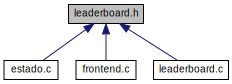
\includegraphics[width=304pt]{leaderboard_8h__dep__incl}
\end{center}
\end{figure}
\subsection*{Macros}
\begin{DoxyCompactItemize}
\item 
\hypertarget{leaderboard_8h_ab5c9e28069b9fbddd9c296f14d25b84c}{\#define \hyperlink{leaderboard_8h_ab5c9e28069b9fbddd9c296f14d25b84c}{M\+A\+X\+\_\+\+S}~50}\label{leaderboard_8h_ab5c9e28069b9fbddd9c296f14d25b84c}

\begin{DoxyCompactList}\small\item\em Tamanho máximo de uma string que utilizador. \end{DoxyCompactList}\end{DoxyCompactItemize}
\subsection*{Typedefs}
\begin{DoxyCompactItemize}
\item 
\hypertarget{leaderboard_8h_a1b75417d96e36e635a0302644a6c66fc}{typedef struct \hyperlink{structinfo}{info} $\ast$ \hyperlink{leaderboard_8h_a1b75417d96e36e635a0302644a6c66fc}{I\+N\+F\+O}}\label{leaderboard_8h_a1b75417d96e36e635a0302644a6c66fc}

\begin{DoxyCompactList}\small\item\em Estrutura onde é guardada a informação usada pela leaderboard. \end{DoxyCompactList}\end{DoxyCompactItemize}
\subsection*{Functions}
\begin{DoxyCompactItemize}
\item 
char $\ast$ \hyperlink{leaderboard_8h_afead7e22f6585d03b4f9b09d89dfade7}{get\+Info\+\_\+user} (\hyperlink{leaderboard_8c_ae0cd0677a19c7077f6bba18c8276576e}{I\+N\+F\+O} v, int i)
\begin{DoxyCompactList}\small\item\em Função que obtêm o utilizador associado a um bloco de informação. \end{DoxyCompactList}\item 
int \hyperlink{leaderboard_8h_a3596e9737c2017c08210285adbf50541}{get\+Info\+\_\+wins} (\hyperlink{leaderboard_8c_ae0cd0677a19c7077f6bba18c8276576e}{I\+N\+F\+O} v, int i)
\begin{DoxyCompactList}\small\item\em Função que obtêm o número de vitórias associado a um bloco de informação. \end{DoxyCompactList}\item 
int \hyperlink{leaderboard_8h_a6b7ea262cb48cc841d5ba76db2984768}{get\+\_\+info} (\hyperlink{leaderboard_8c_ae0cd0677a19c7077f6bba18c8276576e}{I\+N\+F\+O} $\ast$v, int N)
\begin{DoxyCompactList}\small\item\em Função que indica um array de {\ttfamily I\+N\+F\+O} contendo a leaderboard. \end{DoxyCompactList}\item 
void \hyperlink{leaderboard_8h_aa23db304e56c4f0e17bb06e619fe6956}{push\+\_\+info} (char $\ast$user, int wins)
\begin{DoxyCompactList}\small\item\em Função que adiciona nova informação ao ficheiro. Consoante o utilizador e o número de vitória coloca no ficheiro {\ttfamily D\+I\+R\+I\+N\+F\+O} a informação passada como argumento. Da seguinte forma\+: \end{DoxyCompactList}\end{DoxyCompactItemize}


\subsection{Detailed Description}
Módulo de obtenção da leaderboard. 



\subsection{Function Documentation}
\hypertarget{leaderboard_8h_a6b7ea262cb48cc841d5ba76db2984768}{\index{leaderboard.\+h@{leaderboard.\+h}!get\+\_\+info@{get\+\_\+info}}
\index{get\+\_\+info@{get\+\_\+info}!leaderboard.\+h@{leaderboard.\+h}}
\subsubsection[{get\+\_\+info}]{\setlength{\rightskip}{0pt plus 5cm}int get\+\_\+info (
\begin{DoxyParamCaption}
\item[{{\bf I\+N\+F\+O} $\ast$}]{v, }
\item[{int}]{N}
\end{DoxyParamCaption}
)}}\label{leaderboard_8h_a6b7ea262cb48cc841d5ba76db2984768}


Função que indica um array de {\ttfamily I\+N\+F\+O} contendo a leaderboard. 


\begin{DoxyParams}{Parameters}
{\em v} & Apontador para o endereço onde irá ser colocada a leaderboard. \\
\hline
{\em N} & Número máximo de elementos colocados.\\
\hline
\end{DoxyParams}
\begin{DoxyReturn}{Returns}
Números de elementos colocados.
\end{DoxyReturn}
\begin{DoxySeeAlso}{See also}
\hyperlink{leaderboard_8c_a57f19b982e416216fe5865738c7e5b2a}{list\+\_\+info} 

\hyperlink{leaderboard_8c_a31d353bb4c3a5c08b568d5b5a4e98696}{sort\+\_\+info} 

\hyperlink{leaderboard_8c_ae0cd0677a19c7077f6bba18c8276576e}{I\+N\+F\+O} 
\end{DoxySeeAlso}
\hypertarget{leaderboard_8h_afead7e22f6585d03b4f9b09d89dfade7}{\index{leaderboard.\+h@{leaderboard.\+h}!get\+Info\+\_\+user@{get\+Info\+\_\+user}}
\index{get\+Info\+\_\+user@{get\+Info\+\_\+user}!leaderboard.\+h@{leaderboard.\+h}}
\subsubsection[{get\+Info\+\_\+user}]{\setlength{\rightskip}{0pt plus 5cm}char$\ast$ get\+Info\+\_\+user (
\begin{DoxyParamCaption}
\item[{{\bf I\+N\+F\+O}}]{v, }
\item[{int}]{i}
\end{DoxyParamCaption}
)}}\label{leaderboard_8h_afead7e22f6585d03b4f9b09d89dfade7}


Função que obtêm o utilizador associado a um bloco de informação. 


\begin{DoxyParams}{Parameters}
{\em v} & Array de onde irá ser retirada a informação. \\
\hline
{\em i} & Posição da informação.\\
\hline
\end{DoxyParams}
\begin{DoxyReturn}{Returns}
Devolve o utilizador. 
\end{DoxyReturn}
\hypertarget{leaderboard_8h_a3596e9737c2017c08210285adbf50541}{\index{leaderboard.\+h@{leaderboard.\+h}!get\+Info\+\_\+wins@{get\+Info\+\_\+wins}}
\index{get\+Info\+\_\+wins@{get\+Info\+\_\+wins}!leaderboard.\+h@{leaderboard.\+h}}
\subsubsection[{get\+Info\+\_\+wins}]{\setlength{\rightskip}{0pt plus 5cm}int get\+Info\+\_\+wins (
\begin{DoxyParamCaption}
\item[{{\bf I\+N\+F\+O}}]{v, }
\item[{int}]{i}
\end{DoxyParamCaption}
)}}\label{leaderboard_8h_a3596e9737c2017c08210285adbf50541}


Função que obtêm o número de vitórias associado a um bloco de informação. 


\begin{DoxyParams}{Parameters}
{\em v} & Array de onde irá ser retirada a informação. \\
\hline
{\em i} & Posição da informação.\\
\hline
\end{DoxyParams}
\begin{DoxyReturn}{Returns}
Devolve o número de vitórias. 
\end{DoxyReturn}
\hypertarget{leaderboard_8h_aa23db304e56c4f0e17bb06e619fe6956}{\index{leaderboard.\+h@{leaderboard.\+h}!push\+\_\+info@{push\+\_\+info}}
\index{push\+\_\+info@{push\+\_\+info}!leaderboard.\+h@{leaderboard.\+h}}
\subsubsection[{push\+\_\+info}]{\setlength{\rightskip}{0pt plus 5cm}void push\+\_\+info (
\begin{DoxyParamCaption}
\item[{char $\ast$}]{user, }
\item[{int}]{wins}
\end{DoxyParamCaption}
)}}\label{leaderboard_8h_aa23db304e56c4f0e17bb06e619fe6956}


Função que adiciona nova informação ao ficheiro. Consoante o utilizador e o número de vitória coloca no ficheiro {\ttfamily D\+I\+R\+I\+N\+F\+O} a informação passada como argumento. Da seguinte forma\+: 


\begin{DoxyItemize}
\item Se o utilizador não existir no ficheiro então é colocado no fim.
\item Se o utilizador existir no ficheiro então o seu número de vitórias é atualizado.
\end{DoxyItemize}


\begin{DoxyParams}{Parameters}
{\em user} & Utilizador em registo. \\
\hline
{\em wins} & Nome de vitórias em registo.\\
\hline
\end{DoxyParams}
\begin{DoxySeeAlso}{See also}
\hyperlink{leaderboard_8c_ada70e23e1c8bd904bd090ff8f9d03966}{make\+\_\+info} 

\hyperlink{leaderboard_8c_a9b18aaa9c44ed30a23fcf8811d4c2763}{D\+I\+R\+I\+N\+F\+O} 
\end{DoxySeeAlso}

\hypertarget{parser_8c}{\section{parser.\+c File Reference}
\label{parser_8c}\index{parser.\+c@{parser.\+c}}
}


Módulo de User input / Interpertador de comandos.  


{\ttfamily \#include \char`\"{}estado.\+h\char`\"{}}\\*
{\ttfamily \#include \char`\"{}frontend.\+h\char`\"{}}\\*
{\ttfamily \#include \char`\"{}stdlib.\+h\char`\"{}}\\*
{\ttfamily \#include \char`\"{}stdio.\+h\char`\"{}}\\*
{\ttfamily \#include $<$string.\+h$>$}\\*
{\ttfamily \#include \char`\"{}userfiles.\+h\char`\"{}}\\*
{\ttfamily \#include \char`\"{}decide.\+h\char`\"{}}\\*
{\ttfamily \#include \char`\"{}filemanager.\+h\char`\"{}}\\*
{\ttfamily \#include \char`\"{}state.\+h\char`\"{}}\\*
{\ttfamily \#include \char`\"{}solver.\+h\char`\"{}}\\*
{\ttfamily \#include \char`\"{}givehelp.\+h\char`\"{}}\\*
Include dependency graph for parser.\+c\+:
\nopagebreak
\begin{figure}[H]
\begin{center}
\leavevmode
\includegraphics[width=350pt]{parser_8c__incl}
\end{center}
\end{figure}
\subsection*{Macros}
\begin{DoxyCompactItemize}
\item 
\hypertarget{parser_8c_ae2e06e355435bed377eb689dd5eeaaba}{\#define \hyperlink{parser_8c_ae2e06e355435bed377eb689dd5eeaaba}{tab\+Size}~800}\label{parser_8c_ae2e06e355435bed377eb689dd5eeaaba}

\begin{DoxyCompactList}\small\item\em Macro para o tamanho da área a desenhar. \end{DoxyCompactList}\end{DoxyCompactItemize}
\subsection*{Functions}
\begin{DoxyCompactItemize}
\item 
void \hyperlink{parser_8c_a34976bb9db8f4c74909c52a61a7982eb}{pipe\+\_\+env} (void)
\begin{DoxyCompactList}\small\item\em Efetua todas as operações necessárias para load do utilizador e aplicação dos comandos. \end{DoxyCompactList}\item 
static int \hyperlink{parser_8c_a0da69644ab20507560818f1895e8a481}{main\+\_\+op} (\hyperlink{estado_8c_afbffb4e9c242f93d5a2d607754ce2db8}{E\+S\+T\+A\+D\+O} e, char $\ast$command)
\begin{DoxyCompactList}\small\item\em Efetua a leitura de comandos considerados com principais. \end{DoxyCompactList}\item 
static void \hyperlink{parser_8c_a9dd3ff6aa5721874cf88bec4955f600b}{snd\+\_\+op} (\hyperlink{estado_8c_afbffb4e9c242f93d5a2d607754ce2db8}{E\+S\+T\+A\+D\+O} e, char $\ast$command)
\begin{DoxyCompactList}\small\item\em Efetua a leitura de comandos considerados como secundários. \end{DoxyCompactList}\item 
static int \hyperlink{parser_8c_a227e8f8f6042cf524b17e865a2f4b69c}{get\+\_\+resize} (\hyperlink{estado_8c_afbffb4e9c242f93d5a2d607754ce2db8}{E\+S\+T\+A\+D\+O} e, char $\ast$command)
\begin{DoxyCompactList}\small\item\em Efetua a leitura do tipo de resize que se pretende fazer à grelha do tabuleiro. \end{DoxyCompactList}\item 
static int \hyperlink{parser_8c_a6387331e4edbe1b6e46e442dca2d0e9e}{read\+\_\+menu} (\hyperlink{estado_8c_afbffb4e9c242f93d5a2d607754ce2db8}{E\+S\+T\+A\+D\+O} e, char $\ast$command)
\begin{DoxyCompactList}\small\item\em Efetua a leitura do menu para o qual se pretende alterar. \end{DoxyCompactList}\item 
static int \hyperlink{parser_8c_a963f4a94599302cf043cb1193fc2265b}{choose\+\_\+load} (\hyperlink{estado_8c_afbffb4e9c242f93d5a2d607754ce2db8}{E\+S\+T\+A\+D\+O} e, char $\ast$command)
\begin{DoxyCompactList}\small\item\em Consoante o comando passado na {\bfseries Q\+U\+E\+R\+Y\+\_\+\+S\+T\+R\+I\+N\+G} decide que tipo de load terá de ser feito. \end{DoxyCompactList}\item 
static void \hyperlink{parser_8c_a73656ae8b230927c5daf8aeb07c0fb92}{load\+\_\+map} (\hyperlink{estado_8c_afbffb4e9c242f93d5a2d607754ce2db8}{E\+S\+T\+A\+D\+O} e, char $\ast$command)
\begin{DoxyCompactList}\small\item\em Efetua load de um mapa criado pelo utilizador ao contrário de load\+\_\+id. \end{DoxyCompactList}\item 
static void \hyperlink{parser_8c_a50e4e28b0321b1cf9fd88f166787b4c2}{load\+\_\+id} (\hyperlink{estado_8c_afbffb4e9c242f93d5a2d607754ce2db8}{E\+S\+T\+A\+D\+O} e, char $\ast$command)
\begin{DoxyCompactList}\small\item\em Efetua load do mapa guardado em ficheiro. \end{DoxyCompactList}\item 
\hypertarget{parser_8c_a2ec62418632fae2aa57609082f11fdd7}{static int \hyperlink{parser_8c_a2ec62418632fae2aa57609082f11fdd7}{load\+\_\+random} (\hyperlink{estado_8c_afbffb4e9c242f93d5a2d607754ce2db8}{E\+S\+T\+A\+D\+O} e, char $\ast$name)}\label{parser_8c_a2ec62418632fae2aa57609082f11fdd7}

\begin{DoxyCompactList}\small\item\em Efetua load de um mapa gerado aleatoriamente, anteriormente. \end{DoxyCompactList}\item 
static int \hyperlink{parser_8c_ac8e0d98f52835e13cdeb0815f76693f7}{make\+Play} (\hyperlink{estado_8c_afbffb4e9c242f93d5a2d607754ce2db8}{E\+S\+T\+A\+D\+O} e, char $\ast$command)
\begin{DoxyCompactList}\small\item\em Consoante um comando, efetua um jogada em um dado {\ttfamily E\+S\+T\+A\+D\+O}. \end{DoxyCompactList}\item 
static int \hyperlink{parser_8c_a39d22eae9933bec99ed863c6723abbf4}{read\+Parse} (char $\ast$command, int $\ast$i, int $\ast$j)
\begin{DoxyCompactList}\small\item\em Obtem os valores passados no comando de jogada. \end{DoxyCompactList}\item 
static \hyperlink{estado_8c_afbffb4e9c242f93d5a2d607754ce2db8}{E\+S\+T\+A\+D\+O} \hyperlink{parser_8c_a62404024039935a10aa34e9939a02d4e}{load\+\_\+user} (char $\ast$user)
\begin{DoxyCompactList}\small\item\em Efetua o load do {\ttfamily E\+S\+T\+A\+D\+O} associado a um certo utilizador. \end{DoxyCompactList}\item 
static char $\ast$ \hyperlink{parser_8c_a6d68c2d1184f8a61f809f29b38e743ac}{put\+\_\+user} (char $\ast$user\+Query)
\begin{DoxyCompactList}\small\item\em Identifica em que posição de encontra o identificador do utilizador. \end{DoxyCompactList}\item 
static char $\ast$ \hyperlink{parser_8c_a0d2b502d56325f9e1a72c703c2f51086}{convert} (char $\ast$ler)
\begin{DoxyCompactList}\small\item\em Faz a conversão de uma string de forma a poder ser lida pela função get\+User\+C. \end{DoxyCompactList}\item 
static int \hyperlink{parser_8c_a2ba3af7ad2c8720dffb2e60ec1936697}{get\+User\+C} (char $\ast$query, char $\ast$user, char $\ast$command)
\begin{DoxyCompactList}\small\item\em Identifica o utilizador e o comando a ser executado. \end{DoxyCompactList}\end{DoxyCompactItemize}


\subsection{Detailed Description}
Módulo de User input / Interpertador de comandos. 



\subsection{Function Documentation}
\hypertarget{parser_8c_a963f4a94599302cf043cb1193fc2265b}{\index{parser.\+c@{parser.\+c}!choose\+\_\+load@{choose\+\_\+load}}
\index{choose\+\_\+load@{choose\+\_\+load}!parser.\+c@{parser.\+c}}
\subsubsection[{choose\+\_\+load}]{\setlength{\rightskip}{0pt plus 5cm}static int choose\+\_\+load (
\begin{DoxyParamCaption}
\item[{{\bf E\+S\+T\+A\+D\+O}}]{e, }
\item[{char $\ast$}]{command}
\end{DoxyParamCaption}
)\hspace{0.3cm}{\ttfamily [static]}}}\label{parser_8c_a963f4a94599302cf043cb1193fc2265b}


Consoante o comando passado na {\bfseries Q\+U\+E\+R\+Y\+\_\+\+S\+T\+R\+I\+N\+G} decide que tipo de load terá de ser feito. 


\begin{DoxyParams}{Parameters}
{\em e} & {\ttfamily E\+S\+T\+A\+D\+O} onde terá de ser colocada a grelha. \\
\hline
{\em command} & Comando obtido da {\bfseries Q\+U\+E\+R\+Y\+\_\+\+S\+T\+R\+I\+N\+G}.\\
\hline
\end{DoxyParams}
\begin{DoxyReturn}{Returns}
1 se o comando corresponde à nomenclatura de algum load, 0 caso contrário.
\end{DoxyReturn}
\begin{DoxySeeAlso}{See also}
\hyperlink{parser_8c_a73656ae8b230927c5daf8aeb07c0fb92}{load\+\_\+map} 

\hyperlink{parser_8c_a50e4e28b0321b1cf9fd88f166787b4c2}{load\+\_\+id} 
\end{DoxySeeAlso}
\hypertarget{parser_8c_a0d2b502d56325f9e1a72c703c2f51086}{\index{parser.\+c@{parser.\+c}!convert@{convert}}
\index{convert@{convert}!parser.\+c@{parser.\+c}}
\subsubsection[{convert}]{\setlength{\rightskip}{0pt plus 5cm}static char $\ast$ convert (
\begin{DoxyParamCaption}
\item[{char $\ast$}]{ler}
\end{DoxyParamCaption}
)\hspace{0.3cm}{\ttfamily [static]}}}\label{parser_8c_a0d2b502d56325f9e1a72c703c2f51086}


Faz a conversão de uma string de forma a poder ser lida pela função get\+User\+C. 

A função converte todas as ocorrências de {\bfseries '/'} e {\bfseries '\+\_\+'} em espaços, pois só desta forma é possível ser lida.


\begin{DoxyParams}{Parameters}
{\em ler} & A string que irá converter.\\
\hline
\end{DoxyParams}
\begin{DoxyReturn}{Returns}
A própria string. 
\end{DoxyReturn}
\hypertarget{parser_8c_a227e8f8f6042cf524b17e865a2f4b69c}{\index{parser.\+c@{parser.\+c}!get\+\_\+resize@{get\+\_\+resize}}
\index{get\+\_\+resize@{get\+\_\+resize}!parser.\+c@{parser.\+c}}
\subsubsection[{get\+\_\+resize}]{\setlength{\rightskip}{0pt plus 5cm}static int get\+\_\+resize (
\begin{DoxyParamCaption}
\item[{{\bf E\+S\+T\+A\+D\+O}}]{e, }
\item[{char $\ast$}]{command}
\end{DoxyParamCaption}
)\hspace{0.3cm}{\ttfamily [static]}}}\label{parser_8c_a227e8f8f6042cf524b17e865a2f4b69c}


Efetua a leitura do tipo de resize que se pretende fazer à grelha do tabuleiro. 


\begin{DoxyParams}{Parameters}
{\em e} & {\ttfamily E\+S\+T\+A\+D\+O} que irá ser alterado. \\
\hline
{\em command} & Comando obtido da {\bfseries Q\+U\+E\+R\+Y\+\_\+\+S\+T\+R\+I\+N\+G}.\\
\hline
\end{DoxyParams}
\begin{DoxyReturn}{Returns}
1 se o tamanho de grelha foi alterado, 0 caso contrário.
\end{DoxyReturn}
\begin{DoxySeeAlso}{See also}
\hyperlink{state_8h_a1bee768ce8693d3a440b5a60b545dce3}{increase} 
\end{DoxySeeAlso}
\hypertarget{parser_8c_a2ba3af7ad2c8720dffb2e60ec1936697}{\index{parser.\+c@{parser.\+c}!get\+User\+C@{get\+User\+C}}
\index{get\+User\+C@{get\+User\+C}!parser.\+c@{parser.\+c}}
\subsubsection[{get\+User\+C}]{\setlength{\rightskip}{0pt plus 5cm}static int get\+User\+C (
\begin{DoxyParamCaption}
\item[{char $\ast$}]{query, }
\item[{char $\ast$}]{user, }
\item[{char $\ast$}]{command}
\end{DoxyParamCaption}
)\hspace{0.3cm}{\ttfamily [static]}}}\label{parser_8c_a2ba3af7ad2c8720dffb2e60ec1936697}


Identifica o utilizador e o comando a ser executado. 

Identifica, caso existam, o utilizador e o comando passado na {\bfseries Q\+U\+E\+R\+Y\+\_\+\+S\+T\+R\+I\+N\+G}.


\begin{DoxyParams}{Parameters}
{\em query} & {\bfseries Q\+U\+E\+R\+Y} de onde se irá retirar o utilizador e o comando. \\
\hline
{\em user} & Apontador de onde irá ser colocado o utilizador passado na {\bfseries Q\+U\+E\+R\+Y} \\
\hline
{\em command} & Apontador de onde irá ser colocado o comando passado na {\bfseries Q\+U\+E\+R\+Y}.\\
\hline
\end{DoxyParams}
\begin{DoxyReturn}{Returns}
O número de inputs lidos com sucesso. 
\end{DoxyReturn}
\hypertarget{parser_8c_a50e4e28b0321b1cf9fd88f166787b4c2}{\index{parser.\+c@{parser.\+c}!load\+\_\+id@{load\+\_\+id}}
\index{load\+\_\+id@{load\+\_\+id}!parser.\+c@{parser.\+c}}
\subsubsection[{load\+\_\+id}]{\setlength{\rightskip}{0pt plus 5cm}static void load\+\_\+id (
\begin{DoxyParamCaption}
\item[{{\bf E\+S\+T\+A\+D\+O}}]{e, }
\item[{char $\ast$}]{command}
\end{DoxyParamCaption}
)\hspace{0.3cm}{\ttfamily [static]}}}\label{parser_8c_a50e4e28b0321b1cf9fd88f166787b4c2}


Efetua load do mapa guardado em ficheiro. 

Lê o mapa contido em ficheiro, fazendo a verificação da sua validade, e se este for válido, coloca em {\ttfamily e} a grelha correspondente. Caso contrário, coloca o utilizador no menu de mapa inválido.


\begin{DoxyParams}{Parameters}
{\em e} & {\ttfamily E\+S\+T\+A\+D\+O} onde irá ser colocada a grelha lida. \\
\hline
{\em command} & String correspondente ao comando passado na {\bfseries Q\+U\+E\+R\+Y\+\_\+\+S\+T\+R\+I\+N\+G}.\\
\hline
\end{DoxyParams}
\begin{DoxySeeAlso}{See also}
\hyperlink{filemanager_8h_a65db46ec06db54c143d8c58f50a480af}{S\+E\+L\+E\+C\+T} 

\hyperlink{estado_8h_aa7a928e6dc71c7e6f4e25da3b5c10006}{set\+E\+\_\+state} 

\hyperlink{estado_8h_a173aba83ee9ef88015706361de32ae1d}{set\+E\+\_\+menu} 

\hyperlink{estado_8h_a8b28e51aaf0dded437325daee1e86238}{destroy\+State} 
\end{DoxySeeAlso}
\hypertarget{parser_8c_a73656ae8b230927c5daf8aeb07c0fb92}{\index{parser.\+c@{parser.\+c}!load\+\_\+map@{load\+\_\+map}}
\index{load\+\_\+map@{load\+\_\+map}!parser.\+c@{parser.\+c}}
\subsubsection[{load\+\_\+map}]{\setlength{\rightskip}{0pt plus 5cm}static void load\+\_\+map (
\begin{DoxyParamCaption}
\item[{{\bf E\+S\+T\+A\+D\+O}}]{e, }
\item[{char $\ast$}]{command}
\end{DoxyParamCaption}
)\hspace{0.3cm}{\ttfamily [static]}}}\label{parser_8c_a73656ae8b230927c5daf8aeb07c0fb92}


Efetua load de um mapa criado pelo utilizador ao contrário de load\+\_\+id. 

Lê a grelha contida em ficheiro, e caso esta seja válida e se encontre no formato pedido, então esta é colocada no {\ttfamily E\+S\+T\+A\+D\+O} {\ttfamily e} passado como argumento.


\begin{DoxyParams}{Parameters}
{\em e} & {\ttfamily E\+S\+T\+A\+D\+O} onde irá ser colocada a grelha. \\
\hline
{\em command} & Comando passado da {\bfseries Q\+U\+E\+R\+Y\+\_\+\+S\+T\+R\+I\+N\+G}.\\
\hline
\end{DoxyParams}
\begin{DoxySeeAlso}{See also}
\hyperlink{filemanager_8h_a312709802aca1cafd23ab379fb6fb9cc}{s\+Padrao} 

\hyperlink{estado_8h_aa7a928e6dc71c7e6f4e25da3b5c10006}{set\+E\+\_\+state} 

\hyperlink{estado_8h_a8b28e51aaf0dded437325daee1e86238}{destroy\+State} 

\hyperlink{estado_8h_a173aba83ee9ef88015706361de32ae1d}{set\+E\+\_\+menu} 

\hyperlink{estado_8h_a37030bdeb38ad57caa19d47f541f14f3}{set\+E\+\_\+help} 

\hyperlink{parser_8c_a50e4e28b0321b1cf9fd88f166787b4c2}{load\+\_\+id} 
\end{DoxySeeAlso}
\hypertarget{parser_8c_a62404024039935a10aa34e9939a02d4e}{\index{parser.\+c@{parser.\+c}!load\+\_\+user@{load\+\_\+user}}
\index{load\+\_\+user@{load\+\_\+user}!parser.\+c@{parser.\+c}}
\subsubsection[{load\+\_\+user}]{\setlength{\rightskip}{0pt plus 5cm}static {\bf E\+S\+T\+A\+D\+O} load\+\_\+user (
\begin{DoxyParamCaption}
\item[{char $\ast$}]{user}
\end{DoxyParamCaption}
)\hspace{0.3cm}{\ttfamily [static]}}}\label{parser_8c_a62404024039935a10aa34e9939a02d4e}


Efetua o load do {\ttfamily E\+S\+T\+A\+D\+O} associado a um certo utilizador. 

Cria o {\ttfamily E\+S\+T\+A\+D\+O} guardado em ficheiro de um certo utilizador, ou caso este não exista, cria um novo {\ttfamily E\+S\+T\+A\+D\+O} que será associado ao utilizador passado como argumentos.


\begin{DoxyParams}{Parameters}
{\em user} & O utilizador do qual se pretende fazer load.\\
\hline
\end{DoxyParams}
\begin{DoxyReturn}{Returns}
O {\ttfamily E\+S\+T\+A\+D\+O} lido.
\end{DoxyReturn}
\begin{DoxySeeAlso}{See also}
\hyperlink{parser_8c_a6d68c2d1184f8a61f809f29b38e743ac}{put\+\_\+user} 

\hyperlink{userfiles_8h_a698a8661109d5789f2b856cdf3b22adb}{file2estado} 

\hyperlink{estado_8h_a1c52197ddde667791a5210fd441cd3dc}{inicializar} 

\hyperlink{estado_8h_a173aba83ee9ef88015706361de32ae1d}{set\+E\+\_\+menu} 
\end{DoxySeeAlso}
\hypertarget{parser_8c_a0da69644ab20507560818f1895e8a481}{\index{parser.\+c@{parser.\+c}!main\+\_\+op@{main\+\_\+op}}
\index{main\+\_\+op@{main\+\_\+op}!parser.\+c@{parser.\+c}}
\subsubsection[{main\+\_\+op}]{\setlength{\rightskip}{0pt plus 5cm}static int main\+\_\+op (
\begin{DoxyParamCaption}
\item[{{\bf E\+S\+T\+A\+D\+O}}]{e, }
\item[{char $\ast$}]{command}
\end{DoxyParamCaption}
)\hspace{0.3cm}{\ttfamily [static]}}}\label{parser_8c_a0da69644ab20507560818f1895e8a481}


Efetua a leitura de comandos considerados com principais. 

Estes comandos mais importantes correspondem aos seguintes\+:


\begin{DoxyItemize}
\item Efetuar uma jogada na grelha.
\item Efetuar operações de redimensão.
\item Alterar o menu do {\ttfamily E\+S\+T\+A\+D\+O}.
\item Fazer load de uma grelha guardada em ficheiro.
\end{DoxyItemize}


\begin{DoxyParams}{Parameters}
{\em e} & {\ttfamily E\+S\+T\+A\+D\+O} que irá ser alterado. \\
\hline
{\em command} & Comando passado na {\bfseries Q\+U\+E\+R\+Y\+\_\+\+S\+T\+R\+I\+N\+G}.\\
\hline
\end{DoxyParams}
\begin{DoxyReturn}{Returns}
1 se o estado foi alterado, 0 caso contrário.
\end{DoxyReturn}
\begin{DoxySeeAlso}{See also}
\hyperlink{parser_8c_ac8e0d98f52835e13cdeb0815f76693f7}{make\+Play} 

\hyperlink{parser_8c_a227e8f8f6042cf524b17e865a2f4b69c}{get\+\_\+resize} 

\hyperlink{parser_8c_a6387331e4edbe1b6e46e442dca2d0e9e}{read\+\_\+menu} 

\hyperlink{parser_8c_a963f4a94599302cf043cb1193fc2265b}{choose\+\_\+load} 
\end{DoxySeeAlso}
\hypertarget{parser_8c_ac8e0d98f52835e13cdeb0815f76693f7}{\index{parser.\+c@{parser.\+c}!make\+Play@{make\+Play}}
\index{make\+Play@{make\+Play}!parser.\+c@{parser.\+c}}
\subsubsection[{make\+Play}]{\setlength{\rightskip}{0pt plus 5cm}static int make\+Play (
\begin{DoxyParamCaption}
\item[{{\bf E\+S\+T\+A\+D\+O}}]{e, }
\item[{char $\ast$}]{command}
\end{DoxyParamCaption}
)\hspace{0.3cm}{\ttfamily [static]}}}\label{parser_8c_ac8e0d98f52835e13cdeb0815f76693f7}


Consoante um comando, efetua um jogada em um dado {\ttfamily E\+S\+T\+A\+D\+O}. 

Após os valores da linha e coluna serem lidos do comando, é efetuada a jogada correspondente na posição.


\begin{DoxyParams}{Parameters}
{\em e} & {\ttfamily E\+S\+T\+A\+D\+O} que irá ser alterado. \\
\hline
{\em command} & Comando obtido da {\bfseries Q\+U\+E\+R\+Y\+\_\+\+S\+T\+R\+I\+N\+G}.\\
\hline
\end{DoxyParams}
\begin{DoxyReturn}{Returns}
1 se o {\ttfamily E\+S\+T\+A\+D\+O} foi alterado, 0 caso contrário.
\end{DoxyReturn}
\begin{DoxySeeAlso}{See also}
\hyperlink{parser_8c_a39d22eae9933bec99ed863c6723abbf4}{read\+Parse} 

\hyperlink{decide_8h_a82c09231e65f427fb432011ca6e79ad1}{play\+Pos} 
\end{DoxySeeAlso}
\hypertarget{parser_8c_a34976bb9db8f4c74909c52a61a7982eb}{\index{parser.\+c@{parser.\+c}!pipe\+\_\+env@{pipe\+\_\+env}}
\index{pipe\+\_\+env@{pipe\+\_\+env}!parser.\+c@{parser.\+c}}
\subsubsection[{pipe\+\_\+env}]{\setlength{\rightskip}{0pt plus 5cm}void pipe\+\_\+env (
\begin{DoxyParamCaption}
\item[{void}]{}
\end{DoxyParamCaption}
)}}\label{parser_8c_a34976bb9db8f4c74909c52a61a7982eb}


Efetua todas as operações necessárias para load do utilizador e aplicação dos comandos. 

Para a leitura de utilizadores e comandos há três situações, consoante o número de itens lidos.


\begin{DoxyItemize}
\item Caso nenhum item seja lido, então é colocada na página uma input box onde se deve colocar o utilizador.
\item Caso seja só lido o utilizador, é aberto o {\ttfamily E\+S\+T\+A\+D\+O} correspondente e apresentado.
\item Caso seja lido o utilizador e o comando, é apresentado o {\ttfamily E\+S\+T\+A\+D\+O} corresponde com as alterações do comando já efetuadas.
\begin{DoxyItemize}
\item Neste caso acima, primeiro são analisadas as operações principais, e caso nenhuma seja efetuada, então passa para as operações secundárias.
\end{DoxyItemize}
\end{DoxyItemize}

No final, o {\ttfamily E\+S\+T\+A\+D\+O} é escrito em ficheiro.

\begin{DoxySeeAlso}{See also}
\hyperlink{parser_8c_a2ba3af7ad2c8720dffb2e60ec1936697}{get\+User\+C} 

\hyperlink{parser_8c_a0d2b502d56325f9e1a72c703c2f51086}{convert} 

\hyperlink{frontend_8h_a24cc4ee047b57331edabed32f639b9f7}{select\+File} 

\hyperlink{parser_8c_a62404024039935a10aa34e9939a02d4e}{load\+\_\+user} 

\hyperlink{parser_8c_a0da69644ab20507560818f1895e8a481}{main\+\_\+op} 

\hyperlink{parser_8c_a9dd3ff6aa5721874cf88bec4955f600b}{snd\+\_\+op} 

\hyperlink{userfiles_8h_af94c939d48715fec1933684c3073f7d9}{estado2file} 

\hyperlink{frontend_8h_a3bd06a6350b1adbcf2d2d71769b27ff9}{printstate} 

\hyperlink{estado_8h_a8b28e51aaf0dded437325daee1e86238}{destroy\+State} 
\end{DoxySeeAlso}
\hypertarget{parser_8c_a6d68c2d1184f8a61f809f29b38e743ac}{\index{parser.\+c@{parser.\+c}!put\+\_\+user@{put\+\_\+user}}
\index{put\+\_\+user@{put\+\_\+user}!parser.\+c@{parser.\+c}}
\subsubsection[{put\+\_\+user}]{\setlength{\rightskip}{0pt plus 5cm}static char $\ast$ put\+\_\+user (
\begin{DoxyParamCaption}
\item[{char $\ast$}]{user\+Query}
\end{DoxyParamCaption}
)\hspace{0.3cm}{\ttfamily [static]}}}\label{parser_8c_a6d68c2d1184f8a61f809f29b38e743ac}


Identifica em que posição de encontra o identificador do utilizador. 


\begin{DoxyParams}{Parameters}
{\em user\+Query} & String lida da {\bfseries Q\+U\+E\+R\+Y\+\_\+\+S\+T\+R\+I\+N\+G} correspondente.\\
\hline
\end{DoxyParams}
\begin{DoxyReturn}{Returns}
Posição onde se encontra o identificador do utilizador. 
\end{DoxyReturn}
\hypertarget{parser_8c_a6387331e4edbe1b6e46e442dca2d0e9e}{\index{parser.\+c@{parser.\+c}!read\+\_\+menu@{read\+\_\+menu}}
\index{read\+\_\+menu@{read\+\_\+menu}!parser.\+c@{parser.\+c}}
\subsubsection[{read\+\_\+menu}]{\setlength{\rightskip}{0pt plus 5cm}static int read\+\_\+menu (
\begin{DoxyParamCaption}
\item[{{\bf E\+S\+T\+A\+D\+O}}]{e, }
\item[{char $\ast$}]{command}
\end{DoxyParamCaption}
)\hspace{0.3cm}{\ttfamily [static]}}}\label{parser_8c_a6387331e4edbe1b6e46e442dca2d0e9e}


Efetua a leitura do menu para o qual se pretende alterar. 

A função lê o menu para o qual se pretende alterar e faz a devida alteração, sendo que quando o estado corresponde a M\+E\+N\+U\+\_\+\+I\+N\+D\+E\+X\+::\+S\+E\+L\+E\+C\+T\+\_\+\+M\+E\+N\+U o {\ttfamily E\+S\+T\+A\+D\+O} é inicializado.


\begin{DoxyParams}{Parameters}
{\em e} & {\ttfamily E\+S\+T\+A\+D\+O} que irá ser alterado. \\
\hline
{\em command} & Comando passado na {\bfseries Q\+U\+E\+R\+Y\+\_\+\+S\+T\+R\+I\+N\+G}.\\
\hline
\end{DoxyParams}
\begin{DoxyReturn}{Returns}
1, se o menu foi alterado, 0 caso contrário.
\end{DoxyReturn}
\begin{DoxySeeAlso}{See also}
\hyperlink{estado_8h_a173aba83ee9ef88015706361de32ae1d}{set\+E\+\_\+menu} 

\hyperlink{estado_8h_a6b89af2e2e3e9eaf3521701eec86a702}{get\+E\+\_\+menu} 

\hyperlink{estado_8h_a1c52197ddde667791a5210fd441cd3dc}{inicializar} 
\end{DoxySeeAlso}
\hypertarget{parser_8c_a39d22eae9933bec99ed863c6723abbf4}{\index{parser.\+c@{parser.\+c}!read\+Parse@{read\+Parse}}
\index{read\+Parse@{read\+Parse}!parser.\+c@{parser.\+c}}
\subsubsection[{read\+Parse}]{\setlength{\rightskip}{0pt plus 5cm}static int read\+Parse (
\begin{DoxyParamCaption}
\item[{char $\ast$}]{command, }
\item[{int $\ast$}]{i, }
\item[{int $\ast$}]{j}
\end{DoxyParamCaption}
)\hspace{0.3cm}{\ttfamily [static]}}}\label{parser_8c_a39d22eae9933bec99ed863c6723abbf4}


Obtem os valores passados no comando de jogada. 

Por nomenclatura um comando de jogada, é todo o comando que comece com o caráter '@'.


\begin{DoxyParams}{Parameters}
{\em command} & O comando lido da {\bfseries Q\+U\+E\+R\+Y\+\_\+\+S\+T\+R\+I\+N\+G}. \\
\hline
{\em i} & Apontador onde ira colocar a linha onde se pretende jogar. \\
\hline
{\em j} & Apontador onde ira colocar a coluna onde se pretende jogar.\\
\hline
\end{DoxyParams}
\begin{DoxyReturn}{Returns}
O número de elementos lidos com sucesso. 
\end{DoxyReturn}
\hypertarget{parser_8c_a9dd3ff6aa5721874cf88bec4955f600b}{\index{parser.\+c@{parser.\+c}!snd\+\_\+op@{snd\+\_\+op}}
\index{snd\+\_\+op@{snd\+\_\+op}!parser.\+c@{parser.\+c}}
\subsubsection[{snd\+\_\+op}]{\setlength{\rightskip}{0pt plus 5cm}static void snd\+\_\+op (
\begin{DoxyParamCaption}
\item[{{\bf E\+S\+T\+A\+D\+O}}]{e, }
\item[{char $\ast$}]{command}
\end{DoxyParamCaption}
)\hspace{0.3cm}{\ttfamily [static]}}}\label{parser_8c_a9dd3ff6aa5721874cf88bec4955f600b}


Efetua a leitura de comandos considerados como secundários. 

Efetua a leitura de comandos que são considerados menos importantes em termos de aplicação, e por isso a sua verificação é feita numa só função. Estas funções correspondem aos seguintes comandos.

{\bfseries Comando} \+: {\bfseries Função}.


\begin{DoxyItemize}
\item help \+: givehelp.
\item undo \+: pipestack, com o segundo argumento a 0.
\item redo \+: pipestack, com o segundo argumento a 1.
\item solve \+: solve.
\item clear \+: clearstate.
\item save\+Checkpoint \+: save\+Anc.
\item safedraw \+: safedraw.
\item get\+Anc \+: pop\+\_\+\+Anc.
\item clear\+S \+: clearcanvas.
\end{DoxyItemize}
\begin{DoxyParams}{Parameters}
{\em e} & {\ttfamily E\+S\+T\+A\+D\+O} que irá ser alterado. \\
\hline
{\em command} & Comando obtido da {\bfseries Q\+U\+E\+R\+Y\+\_\+\+S\+T\+R\+I\+N\+G}.\\
\hline
\end{DoxyParams}
\begin{DoxySeeAlso}{See also}
\hyperlink{givehelp_8h_a56fc46f28368685f0897f3f58f80b039}{givehelp} 

\hyperlink{state_8h_ab9caafc0116aeec18705eda9533f132f}{pipestack} 

\hyperlink{solver_8h_a6102730d9741f071f2354149756162a6}{solve} 

\hyperlink{state_8h_a11aed0a30a94f6dbf787a6c73dbd6409}{clearstate} 

\hyperlink{state_8h_a695e69034d7f22ba4eb4489af2e8786c}{save\+Anc} 

\hyperlink{state_8h_abcfe0e950583a81bc2a7586eb7d044b5}{safedraw} 

\hyperlink{state_8h_aa72d6a8965f5d7a3d214a4ecde14ecc0}{pop\+\_\+\+Anc} 

\hyperlink{state_8h_a8f967d9da54fb07016a74353f7a230ee}{clearcanvas} 
\end{DoxySeeAlso}

\hypertarget{parser_8h}{\section{parser.\+h File Reference}
\label{parser_8h}\index{parser.\+h@{parser.\+h}}
}


Ficheiro header de User input / Interpertador de comandos.  


This graph shows which files directly or indirectly include this file\+:
\nopagebreak
\begin{figure}[H]
\begin{center}
\leavevmode
\includegraphics[width=140pt]{parser_8h__dep__incl}
\end{center}
\end{figure}
\subsection*{Functions}
\begin{DoxyCompactItemize}
\item 
void \hyperlink{parser_8h_a34976bb9db8f4c74909c52a61a7982eb}{pipe\+\_\+env} (void)
\begin{DoxyCompactList}\small\item\em Efetua todas as operações necessárias para load do utilizador e aplicação dos comandos. \end{DoxyCompactList}\end{DoxyCompactItemize}


\subsection{Detailed Description}
Ficheiro header de User input / Interpertador de comandos. 



\subsection{Function Documentation}
\hypertarget{parser_8h_a34976bb9db8f4c74909c52a61a7982eb}{\index{parser.\+h@{parser.\+h}!pipe\+\_\+env@{pipe\+\_\+env}}
\index{pipe\+\_\+env@{pipe\+\_\+env}!parser.\+h@{parser.\+h}}
\subsubsection[{pipe\+\_\+env}]{\setlength{\rightskip}{0pt plus 5cm}void pipe\+\_\+env (
\begin{DoxyParamCaption}
\item[{void}]{}
\end{DoxyParamCaption}
)}}\label{parser_8h_a34976bb9db8f4c74909c52a61a7982eb}


Efetua todas as operações necessárias para load do utilizador e aplicação dos comandos. 

Para a leitura de utilizadores e comandos há três situações, consoante o número de itens lidos.


\begin{DoxyItemize}
\item Caso nenhum item seja lido, então é colocada na página uma input box onde se deve colocar o utilizador.
\item Caso seja só lido o utilizador, é aberto o {\ttfamily E\+S\+T\+A\+D\+O} correspondente e apresentado.
\item Caso seja lido o utilizador e o comando, é apresentado o {\ttfamily E\+S\+T\+A\+D\+O} corresponde com as alterações do comando já efetuadas.
\begin{DoxyItemize}
\item Neste caso acima, primeiro são analisadas as operações principais, e caso nenhuma seja efetuada, então passa para as operações secundárias.
\end{DoxyItemize}
\end{DoxyItemize}

No final, o {\ttfamily E\+S\+T\+A\+D\+O} é escrito em ficheiro.

\begin{DoxySeeAlso}{See also}
\hyperlink{parser_8c_a2ba3af7ad2c8720dffb2e60ec1936697}{get\+User\+C} 

\hyperlink{parser_8c_a0d2b502d56325f9e1a72c703c2f51086}{convert} 

\hyperlink{frontend_8h_a24cc4ee047b57331edabed32f639b9f7}{select\+File} 

\hyperlink{parser_8c_a62404024039935a10aa34e9939a02d4e}{load\+\_\+user} 

\hyperlink{parser_8c_a0da69644ab20507560818f1895e8a481}{main\+\_\+op} 

\hyperlink{parser_8c_a9dd3ff6aa5721874cf88bec4955f600b}{snd\+\_\+op} 

\hyperlink{userfiles_8h_af94c939d48715fec1933684c3073f7d9}{estado2file} 

\hyperlink{frontend_8h_a3bd06a6350b1adbcf2d2d71769b27ff9}{printstate} 

\hyperlink{estado_8h_a8b28e51aaf0dded437325daee1e86238}{destroy\+State} 
\end{DoxySeeAlso}

\hypertarget{solver_8c}{\section{solver.\+c File Reference}
\label{solver_8c}\index{solver.\+c@{solver.\+c}}
}


Ficheiro dedicado à análise do espaço de soluções.  


{\ttfamily \#include $<$stdlib.\+h$>$}\\*
{\ttfamily \#include $<$stdio.\+h$>$}\\*
{\ttfamily \#include $<$time.\+h$>$}\\*
{\ttfamily \#include \char`\"{}solver.\+h\char`\"{}}\\*
{\ttfamily \#include $<$string.\+h$>$}\\*
Include dependency graph for solver.\+c\+:
\nopagebreak
\begin{figure}[H]
\begin{center}
\leavevmode
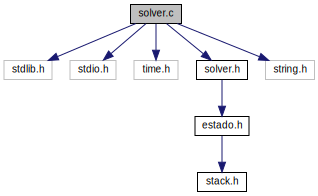
\includegraphics[width=350pt]{solver_8c__incl}
\end{center}
\end{figure}
\subsection*{Classes}
\begin{DoxyCompactItemize}
\item 
struct \hyperlink{structstate}{state}
\begin{DoxyCompactList}\small\item\em Declaração do estado interno. \end{DoxyCompactList}\item 
struct \hyperlink{structgtree}{gtree}
\begin{DoxyCompactList}\small\item\em Estrutura que representa o espaço de soluções de um dado Estado. \end{DoxyCompactList}\item 
struct \hyperlink{structgtree_1_1pecas}{gtree\+::pecas}
\begin{DoxyCompactList}\small\item\em Estrutura que contem apontadores para os filhos do nodo. \end{DoxyCompactList}\end{DoxyCompactItemize}
\subsection*{Macros}
\begin{DoxyCompactItemize}
\item 
\#define \hyperlink{solver_8c_a806da3fd78ef4fa442d053b1c67f58b7}{testall}(x, y, num\+\_\+lins, num\+\_\+cols)~((y $<$ num\+\_\+lins) \&\& (x $<$ num\+\_\+cols) \&\& (x $>$= 0) \&\& (y $>$= 0))
\begin{DoxyCompactList}\small\item\em Macro que verifica se valores se encontram dentro de um intervalo. \end{DoxyCompactList}\item 
\#define \hyperlink{solver_8c_a2d6130b49e818bfe457fb0905176d8f6}{contain}(x1, y1, x2, y2, num\+\_\+lins, num\+\_\+cols)~(\hyperlink{validate_8c_a3e83cfe59dc3bacf9951d6e40cb4ecc7}{testall}(x1, y1, num\+\_\+lins, num\+\_\+cols) \&\& \hyperlink{validate_8c_a3e83cfe59dc3bacf9951d6e40cb4ecc7}{testall}(x2, y2, num\+\_\+lins, num\+\_\+cols))
\begin{DoxyCompactList}\small\item\em Macro que verifica se dua pecas estão dentro do tabuleiro. \end{DoxyCompactList}\item 
\#define \hyperlink{solver_8c_ab27ec55b4939191fcd8573e095c46718}{countval}(x1, y1, x2, y2, \hyperlink{structstate}{state})~(\hyperlink{validate_8c_ad3ddaa88cdf36ed91ed86c882719b023}{equal}(x1, y1, x2, y2, \hyperlink{structstate}{state}) \&\& \hyperlink{validate_8c_a04580bc5cd9cff271e78e4d5645ed293}{ignore}(x1, y1, \hyperlink{structstate}{state}))
\begin{DoxyCompactList}\small\item\em Macro que verifica se duas pecas são iguais e diferentes de V\+A\+Z\+I\+O e B\+L\+O\+Q\+U\+E\+A\+D\+A. \end{DoxyCompactList}\item 
\#define \hyperlink{solver_8c_a30b7bce0ad2f3157f2dc094fffb9a2b1}{ignore}(x, y, \hyperlink{structstate}{state})~((\hyperlink{solver_8c_a4301a2244ca8bec79d38108a18b809f5}{acess}(x, y, \hyperlink{structstate}{state}) != V\+A\+Z\+I\+A) \&\& (\hyperlink{solver_8c_a4301a2244ca8bec79d38108a18b809f5}{acess}(x, y, \hyperlink{structstate}{state}) != B\+L\+O\+Q\+U\+E\+A\+D\+A))
\begin{DoxyCompactList}\small\item\em Macro para verificar se uma posição é diferente de V\+A\+Z\+I\+A e de B\+L\+O\+Q\+U\+E\+A\+D\+A. \end{DoxyCompactList}\item 
\#define \hyperlink{solver_8c_a4301a2244ca8bec79d38108a18b809f5}{acess}(x, y, \hyperlink{structstate}{state})~(\hyperlink{structstate}{state}\mbox{[}x\mbox{]}\mbox{[}y\mbox{]})
\begin{DoxyCompactList}\small\item\em Macro que devolve o valor de uma posição. \end{DoxyCompactList}\item 
\#define \hyperlink{solver_8c_ab391e62015346112bc3af684bead24a0}{equal}(x1, y1, x2, y2, \hyperlink{structstate}{state})~(\hyperlink{solver_8c_a4301a2244ca8bec79d38108a18b809f5}{acess}(x1, y1, \hyperlink{structstate}{state}) == \hyperlink{solver_8c_a4301a2244ca8bec79d38108a18b809f5}{acess}(x2, y2, \hyperlink{structstate}{state}))
\begin{DoxyCompactList}\small\item\em Macro para verificar se duas posições são iguais. \end{DoxyCompactList}\item 
\#define \hyperlink{solver_8c_aff9931d7524c88e07743af6535b20761}{M\+A\+X}(X, Y)~((X) $>$ (Y)) ? (X) \+: (Y)
\begin{DoxyCompactList}\small\item\em Macro para cálculo do valor máximo. \end{DoxyCompactList}\end{DoxyCompactItemize}
\subsection*{Typedefs}
\begin{DoxyCompactItemize}
\item 
\hypertarget{solver_8c_a4eecb6dfe9c84dfb5f547bd0511f6994}{typedef struct \hyperlink{structstate}{state} $\ast$ \hyperlink{solver_8c_a4eecb6dfe9c84dfb5f547bd0511f6994}{T}}\label{solver_8c_a4eecb6dfe9c84dfb5f547bd0511f6994}

\begin{DoxyCompactList}\small\item\em Declaração do estado interno. \end{DoxyCompactList}\item 
\hypertarget{solver_8c_a320d65c31df749caec2f5dbe1a3d3309}{typedef struct \hyperlink{structgtree}{gtree} $\ast$ \hyperlink{solver_8c_a320d65c31df749caec2f5dbe1a3d3309}{G\+Tree}}\label{solver_8c_a320d65c31df749caec2f5dbe1a3d3309}

\begin{DoxyCompactList}\small\item\em Estrutura que representa o espaço de soluções de um dado Estado. \end{DoxyCompactList}\end{DoxyCompactItemize}
\subsection*{Enumerations}
\begin{DoxyCompactItemize}
\item 
enum \hyperlink{solver_8c_a525bf7e52560dc0068ad77c5435af98b}{H\+U\+N\+T} \{ \hyperlink{solver_8c_a525bf7e52560dc0068ad77c5435af98baa57edeeb1dd2c77d5b8afca80b14e9aa}{R\+O\+A\+D}, 
\hyperlink{solver_8c_a525bf7e52560dc0068ad77c5435af98ba2e29f8ab4cef28acccce44e578b257dc}{T\+R\+A\+I\+L}, 
\hyperlink{solver_8c_a525bf7e52560dc0068ad77c5435af98ba7427d7115f5add8d4260333334793dc7}{T\+R\+E\+S\+U\+R\+E}
 \}
\begin{DoxyCompactList}\small\item\em Tipos de nodos de uma G\+Tree. \end{DoxyCompactList}\end{DoxyCompactItemize}
\subsection*{Functions}
\begin{DoxyCompactItemize}
\item 
\hyperlink{estado_8c_afbffb4e9c242f93d5a2d607754ce2db8}{E\+S\+T\+A\+D\+O} \hyperlink{solver_8c_a6102730d9741f071f2354149756162a6}{solve} (\hyperlink{estado_8c_afbffb4e9c242f93d5a2d607754ce2db8}{E\+S\+T\+A\+D\+O} a, long $\ast$number\+\_\+of\+\_\+solutions)
\begin{DoxyCompactList}\small\item\em Resolve um dado E\+S\+T\+A\+D\+O. \end{DoxyCompactList}\item 
\hyperlink{solver_8c_a320d65c31df749caec2f5dbe1a3d3309}{G\+Tree} \hyperlink{solver_8c_a5371b705fa6f1d7e41a42bb6d313280f}{ana} (\hyperlink{solver_8c_a4eecb6dfe9c84dfb5f547bd0511f6994}{T} e, \hyperlink{solver_8h_a03634ec1f096fa2c599deb1491a71bda}{Position\+Selector} func)
\begin{DoxyCompactList}\small\item\em Esta função, um anamorfimo, cria árvores de soluções do estado indicado conforme a função recebida. \end{DoxyCompactList}\item 
int \hyperlink{solver_8c_a5c97af1c1d88b32a051b450225f5a981}{cluster} (\hyperlink{solver_8c_a4eecb6dfe9c84dfb5f547bd0511f6994}{T} e, int u, int $\ast$cp, int sig)
\begin{DoxyCompactList}\small\item\em Esta função implementa uma Position Selector. Este Position Selector foi calibrado para promover clustering para obter estados invalidos o mais rapidamente possivel. \end{DoxyCompactList}\item 
\hyperlink{solver_8c_a4eecb6dfe9c84dfb5f547bd0511f6994}{T} \hyperlink{solver_8c_aa84d7910720fb3f1d65cfc5aef010565}{base\+Map} (int numl, int numc, float prob\+B)
\begin{DoxyCompactList}\small\item\em Esta função cria um estado interno aleatório com o minimo de peças preenchidas possível. \end{DoxyCompactList}\item 
int \hyperlink{solver_8c_aea6b60a620fd32a3087893bbafbd87b1}{findk} (\hyperlink{solver_8c_a320d65c31df749caec2f5dbe1a3d3309}{G\+Tree} node, \hyperlink{solver_8c_a320d65c31df749caec2f5dbe1a3d3309}{G\+Tree} $\ast$v)
\begin{DoxyCompactList}\small\item\em Esta função cria um array de nodos com as peças que levam a uma solução. \end{DoxyCompactList}\item 
void \hyperlink{solver_8c_a62183a083fdfe2c14c18270540695676}{destroy\+G\+Tree} (\hyperlink{solver_8c_a320d65c31df749caec2f5dbe1a3d3309}{G\+Tree} node)
\begin{DoxyCompactList}\small\item\em Destroi uma instância da Árvore que representa o espaço de soluções. \end{DoxyCompactList}\item 
void \hyperlink{solver_8c_aef893a4134b63eeeddadf57d2a89ba85}{pick\+G} (\hyperlink{solver_8c_a4eecb6dfe9c84dfb5f547bd0511f6994}{T} e, \hyperlink{solver_8c_a320d65c31df749caec2f5dbe1a3d3309}{G\+Tree} tr)
\begin{DoxyCompactList}\small\item\em Altera o estado interno por forma a conter o elemento que o nodo contêm. \end{DoxyCompactList}\item 
void \hyperlink{solver_8c_a9befd5c024b5276c08fccb7def98092b}{show\+S} (\hyperlink{solver_8c_a4eecb6dfe9c84dfb5f547bd0511f6994}{T} e)
\begin{DoxyCompactList}\small\item\em Escreve um estado interno no ecra. \end{DoxyCompactList}\item 
void \hyperlink{solver_8c_af632244db4e92b792bac954fde83a795}{write\+Map} (\hyperlink{solver_8c_a4eecb6dfe9c84dfb5f547bd0511f6994}{T} e, char $\ast$difficulty)
\begin{DoxyCompactList}\small\item\em Escreve um mapa em ficheiro. \end{DoxyCompactList}\item 
int \hyperlink{solver_8c_a51385fec0d272f29703ff6dc466d59a3}{count\+Use\+S} (\hyperlink{solver_8c_a4eecb6dfe9c84dfb5f547bd0511f6994}{T} e)
\begin{DoxyCompactList}\small\item\em Consulta o numero de casas que podem ser alterados na grelha do estado interno. \end{DoxyCompactList}\item 
int \hyperlink{solver_8c_a5edd3336bf1a14feae92f81deba546fb}{get\+Dimension} (\hyperlink{solver_8c_a4eecb6dfe9c84dfb5f547bd0511f6994}{T} e)
\begin{DoxyCompactList}\small\item\em Consulta o numero de casas na grelha do estado interno. \end{DoxyCompactList}\item 
void \hyperlink{solver_8c_abc174ddc3e0e8a2994759589328ca810}{destroyit} (\hyperlink{solver_8c_a4eecb6dfe9c84dfb5f547bd0511f6994}{T} e)
\begin{DoxyCompactList}\small\item\em Destroi uma instaância do estado interno. \end{DoxyCompactList}\item 
char $\ast$$\ast$ \hyperlink{solver_8c_a89a52a8604a20c3bd897b5c461b6ca92}{convert\+\_\+external} (\hyperlink{solver_8c_a4eecb6dfe9c84dfb5f547bd0511f6994}{T} e)
\begin{DoxyCompactList}\small\item\em Converte o estado interno numa grelha do estado externo. \end{DoxyCompactList}\item 
static int \hyperlink{solver_8c_a0d9f13ee6341325b731c2e477fa9a399}{verifica} (int x, int y, int vectorx, int vectory, int $\ast$$\ast$\hyperlink{structstate}{state}, int l, int c)
\begin{DoxyCompactList}\small\item\em Verifica se no sentido de um dado vetor em questão tem menos de 3 em linhas. \end{DoxyCompactList}\item 
static int \hyperlink{solver_8c_a4e5c14594936dfc099c1f05726bc9698}{valida} (int x, int y, int $\ast$$\ast$e, int maxl, int maxc)
\begin{DoxyCompactList}\small\item\em Válida se uma dada jogada será valida. \end{DoxyCompactList}\item 
static \hyperlink{solver_8c_a4eecb6dfe9c84dfb5f547bd0511f6994}{T} \hyperlink{solver_8c_a2963dbaf1bb98e88a517ccf1a525e63f}{makeit} (int l, int c)
\begin{DoxyCompactList}\small\item\em Construtor do elemento T(estado interno). \end{DoxyCompactList}\item 
static \hyperlink{solver_8c_a4eecb6dfe9c84dfb5f547bd0511f6994}{T} \hyperlink{solver_8c_ac27cadf2b0541e74e6f4c915db7de3a1}{convert\+\_\+internal} (\hyperlink{estado_8c_afbffb4e9c242f93d5a2d607754ce2db8}{E\+S\+T\+A\+D\+O} a)
\begin{DoxyCompactList}\small\item\em Converte o estado externo num estado interno. \end{DoxyCompactList}\item 
static int \hyperlink{solver_8c_a153a660bbdd5fe29918bfdbfdd3e253d}{find\+Way} (\hyperlink{solver_8c_a4eecb6dfe9c84dfb5f547bd0511f6994}{T} current, \hyperlink{solver_8c_a320d65c31df749caec2f5dbe1a3d3309}{G\+Tree} node, int flag)
\begin{DoxyCompactList}\small\item\em Atribui a current uma das soluções (escolhida aleatóriamente) da árvore dada. \end{DoxyCompactList}\item 
static int \hyperlink{solver_8c_af889ba91bf5bb2fbc4fa4d790867709c}{number\+Ofsolutions} (\hyperlink{solver_8c_a320d65c31df749caec2f5dbe1a3d3309}{G\+Tree} node)
\begin{DoxyCompactList}\small\item\em Calcula o numero de soluções da árvore recebida. \end{DoxyCompactList}\item 
static int \hyperlink{solver_8c_a9e5c9151d4c6e5f8225ce4803c643510}{rec\+Ana} (int n, \hyperlink{solver_8c_a4eecb6dfe9c84dfb5f547bd0511f6994}{T} current, \hyperlink{solver_8c_a320d65c31df749caec2f5dbe1a3d3309}{G\+Tree} $\ast$node, \hyperlink{solver_8h_a03634ec1f096fa2c599deb1491a71bda}{Position\+Selector} func)
\begin{DoxyCompactList}\small\item\em Esta função vai recursivamente inspecionando elementos e desenvolvendo a arvore recebida. \end{DoxyCompactList}\item 
static int \hyperlink{solver_8c_ae6f4a9ace4f041e4725c0bf84ddd4a77}{change\+\_\+aim} (int cd\mbox{[}2\mbox{]}, int lin, int col)
\begin{DoxyCompactList}\small\item\em Esta função define qual a próxima coordenada. \end{DoxyCompactList}\item 
static void \hyperlink{solver_8c_a6fe6ec4013107e13b427e2692d3d0adf}{pick} (\hyperlink{solver_8c_a4eecb6dfe9c84dfb5f547bd0511f6994}{T} e, int i, int j, int value)
\begin{DoxyCompactList}\small\item\em Esta função altera uma das entradas de elemento. \end{DoxyCompactList}\end{DoxyCompactItemize}


\subsection{Detailed Description}
Ficheiro dedicado à análise do espaço de soluções. 



\subsection{Macro Definition Documentation}
\hypertarget{solver_8c_a4301a2244ca8bec79d38108a18b809f5}{\index{solver.\+c@{solver.\+c}!acess@{acess}}
\index{acess@{acess}!solver.\+c@{solver.\+c}}
\subsubsection[{acess}]{\setlength{\rightskip}{0pt plus 5cm}\#define acess(
\begin{DoxyParamCaption}
\item[{}]{x, }
\item[{}]{y, }
\item[{}]{{\bf state}}
\end{DoxyParamCaption}
)~({\bf state}\mbox{[}x\mbox{]}\mbox{[}y\mbox{]})}}\label{solver_8c_a4301a2244ca8bec79d38108a18b809f5}


Macro que devolve o valor de uma posição. 


\begin{DoxyParams}{Parameters}
{\em x} & linha da posição \\
\hline
{\em y} & coluna da posição \\
\hline
{\em state} & estado onde se encontra a peca\\
\hline
\end{DoxyParams}
\begin{DoxyReturn}{Returns}
valor da peca na posição (x,y) 
\end{DoxyReturn}
\hypertarget{solver_8c_a2d6130b49e818bfe457fb0905176d8f6}{\index{solver.\+c@{solver.\+c}!contain@{contain}}
\index{contain@{contain}!solver.\+c@{solver.\+c}}
\subsubsection[{contain}]{\setlength{\rightskip}{0pt plus 5cm}\#define contain(
\begin{DoxyParamCaption}
\item[{}]{x1, }
\item[{}]{y1, }
\item[{}]{x2, }
\item[{}]{y2, }
\item[{}]{num\+\_\+lins, }
\item[{}]{num\+\_\+cols}
\end{DoxyParamCaption}
)~({\bf testall}(x1, y1, num\+\_\+lins, num\+\_\+cols) \&\& {\bf testall}(x2, y2, num\+\_\+lins, num\+\_\+cols))}}\label{solver_8c_a2d6130b49e818bfe457fb0905176d8f6}


Macro que verifica se dua pecas estão dentro do tabuleiro. 


\begin{DoxyParams}{Parameters}
{\em x1} & linha da primeira peca \\
\hline
{\em y1} & coluna da primeira peca \\
\hline
{\em x2} & linha da segunda peca \\
\hline
{\em y2} & coluna da segunda peca \\
\hline
{\em num\+\_\+lins} & valor superior do intervalo para x \\
\hline
{\em num\+\_\+cols} & valor superior do intervalo para y\\
\hline
\end{DoxyParams}
\begin{DoxyReturn}{Returns}
1 se ambas estiverem dentro do tabuleiro, 0 caso contrário 
\end{DoxyReturn}
\hypertarget{solver_8c_ab27ec55b4939191fcd8573e095c46718}{\index{solver.\+c@{solver.\+c}!countval@{countval}}
\index{countval@{countval}!solver.\+c@{solver.\+c}}
\subsubsection[{countval}]{\setlength{\rightskip}{0pt plus 5cm}\#define countval(
\begin{DoxyParamCaption}
\item[{}]{x1, }
\item[{}]{y1, }
\item[{}]{x2, }
\item[{}]{y2, }
\item[{}]{{\bf state}}
\end{DoxyParamCaption}
)~({\bf equal}(x1, y1, x2, y2, {\bf state}) \&\& {\bf ignore}(x1, y1, {\bf state}))}}\label{solver_8c_ab27ec55b4939191fcd8573e095c46718}


Macro que verifica se duas pecas são iguais e diferentes de V\+A\+Z\+I\+O e B\+L\+O\+Q\+U\+E\+A\+D\+A. 


\begin{DoxyParams}{Parameters}
{\em x1} & linha da primeira peca \\
\hline
{\em y1} & coluna da primeira peca \\
\hline
{\em x2} & linha da segunda peca \\
\hline
{\em y2} & coluna da segunda peca \\
\hline
{\em state} & estado onde se encontram as pecas\\
\hline
\end{DoxyParams}
\begin{DoxyReturn}{Returns}
1 se as duas pecas são iguais e diferentes de V\+A\+Z\+I\+O e B\+L\+O\+Q\+U\+E\+A\+D\+A, 0 caso contrário 
\end{DoxyReturn}
\hypertarget{solver_8c_ab391e62015346112bc3af684bead24a0}{\index{solver.\+c@{solver.\+c}!equal@{equal}}
\index{equal@{equal}!solver.\+c@{solver.\+c}}
\subsubsection[{equal}]{\setlength{\rightskip}{0pt plus 5cm}\#define equal(
\begin{DoxyParamCaption}
\item[{}]{x1, }
\item[{}]{y1, }
\item[{}]{x2, }
\item[{}]{y2, }
\item[{}]{{\bf state}}
\end{DoxyParamCaption}
)~({\bf acess}(x1, y1, {\bf state}) == {\bf acess}(x2, y2, {\bf state}))}}\label{solver_8c_ab391e62015346112bc3af684bead24a0}


Macro para verificar se duas posições são iguais. 


\begin{DoxyParams}{Parameters}
{\em x1} & linha da primeira peca \\
\hline
{\em y1} & coluna da primeira peca \\
\hline
{\em x2} & linha da segunda peca \\
\hline
{\em y2} & coluna da segunda peca \\
\hline
{\em state} & estado onde se encontram as pecas\\
\hline
\end{DoxyParams}
\begin{DoxyReturn}{Returns}
1 forem iguais, o se forem diferentes 
\end{DoxyReturn}
\hypertarget{solver_8c_a30b7bce0ad2f3157f2dc094fffb9a2b1}{\index{solver.\+c@{solver.\+c}!ignore@{ignore}}
\index{ignore@{ignore}!solver.\+c@{solver.\+c}}
\subsubsection[{ignore}]{\setlength{\rightskip}{0pt plus 5cm}\#define ignore(
\begin{DoxyParamCaption}
\item[{}]{x, }
\item[{}]{y, }
\item[{}]{{\bf state}}
\end{DoxyParamCaption}
)~(({\bf acess}(x, y, {\bf state}) != V\+A\+Z\+I\+A) \&\& ({\bf acess}(x, y, {\bf state}) != B\+L\+O\+Q\+U\+E\+A\+D\+A))}}\label{solver_8c_a30b7bce0ad2f3157f2dc094fffb9a2b1}


Macro para verificar se uma posição é diferente de V\+A\+Z\+I\+A e de B\+L\+O\+Q\+U\+E\+A\+D\+A. 


\begin{DoxyParams}{Parameters}
{\em x} & linha da posição \\
\hline
{\em y} & coluna da posição \\
\hline
{\em state} & estado onde se encontra a peca\\
\hline
\end{DoxyParams}
\begin{DoxyReturn}{Returns}
1 se for diferente de V\+A\+Z\+I\+A e de B\+L\+O\+Q\+U\+E\+A\+D\+A, 0 caso contrário 
\end{DoxyReturn}
\hypertarget{solver_8c_aff9931d7524c88e07743af6535b20761}{\index{solver.\+c@{solver.\+c}!M\+A\+X@{M\+A\+X}}
\index{M\+A\+X@{M\+A\+X}!solver.\+c@{solver.\+c}}
\subsubsection[{M\+A\+X}]{\setlength{\rightskip}{0pt plus 5cm}\#define M\+A\+X(
\begin{DoxyParamCaption}
\item[{}]{X, }
\item[{}]{Y}
\end{DoxyParamCaption}
)~((X) $>$ (Y)) ? (X) \+: (Y)}}\label{solver_8c_aff9931d7524c88e07743af6535b20761}


Macro para cálculo do valor máximo. 


\begin{DoxyParams}{Parameters}
{\em X} & valor 1 \\
\hline
{\em Y} & valor 2\\
\hline
\end{DoxyParams}
\begin{DoxyReturn}{Returns}
o maior entre X e Y 
\end{DoxyReturn}
\hypertarget{solver_8c_a806da3fd78ef4fa442d053b1c67f58b7}{\index{solver.\+c@{solver.\+c}!testall@{testall}}
\index{testall@{testall}!solver.\+c@{solver.\+c}}
\subsubsection[{testall}]{\setlength{\rightskip}{0pt plus 5cm}\#define testall(
\begin{DoxyParamCaption}
\item[{}]{x, }
\item[{}]{y, }
\item[{}]{num\+\_\+lins, }
\item[{}]{num\+\_\+cols}
\end{DoxyParamCaption}
)~((y $<$ num\+\_\+lins) \&\& (x $<$ num\+\_\+cols) \&\& (x $>$= 0) \&\& (y $>$= 0))}}\label{solver_8c_a806da3fd78ef4fa442d053b1c67f58b7}


Macro que verifica se valores se encontram dentro de um intervalo. 


\begin{DoxyParams}{Parameters}
{\em x} & valor 1 a verificar \\
\hline
{\em y} & valor 2 a verificar \\
\hline
{\em num\+\_\+lins} & valor superior do intervalo para x \\
\hline
{\em num\+\_\+cols} & valor superior do intervalo para y\\
\hline
\end{DoxyParams}
\begin{DoxyReturn}{Returns}
1 se x estiver entre 0 e num\+\_\+lins e y entre 0 e num\+\_\+cols, caso contrário devolve 0 
\end{DoxyReturn}


\subsection{Enumeration Type Documentation}
\hypertarget{solver_8c_a525bf7e52560dc0068ad77c5435af98b}{\index{solver.\+c@{solver.\+c}!H\+U\+N\+T@{H\+U\+N\+T}}
\index{H\+U\+N\+T@{H\+U\+N\+T}!solver.\+c@{solver.\+c}}
\subsubsection[{H\+U\+N\+T}]{\setlength{\rightskip}{0pt plus 5cm}enum {\bf H\+U\+N\+T}}}\label{solver_8c_a525bf7e52560dc0068ad77c5435af98b}


Tipos de nodos de uma G\+Tree. 

\begin{Desc}
\item[Enumerator]\par
\begin{description}
\index{R\+O\+A\+D@{R\+O\+A\+D}!solver.\+c@{solver.\+c}}\index{solver.\+c@{solver.\+c}!R\+O\+A\+D@{R\+O\+A\+D}}\item[{\em 
\hypertarget{solver_8c_a525bf7e52560dc0068ad77c5435af98baa57edeeb1dd2c77d5b8afca80b14e9aa}{R\+O\+A\+D}\label{solver_8c_a525bf7e52560dc0068ad77c5435af98baa57edeeb1dd2c77d5b8afca80b14e9aa}
}]Caminho com várias soluções. \index{T\+R\+A\+I\+L@{T\+R\+A\+I\+L}!solver.\+c@{solver.\+c}}\index{solver.\+c@{solver.\+c}!T\+R\+A\+I\+L@{T\+R\+A\+I\+L}}\item[{\em 
\hypertarget{solver_8c_a525bf7e52560dc0068ad77c5435af98ba2e29f8ab4cef28acccce44e578b257dc}{T\+R\+A\+I\+L}\label{solver_8c_a525bf7e52560dc0068ad77c5435af98ba2e29f8ab4cef28acccce44e578b257dc}
}]Caminnho para uma solução única. \index{T\+R\+E\+S\+U\+R\+E@{T\+R\+E\+S\+U\+R\+E}!solver.\+c@{solver.\+c}}\index{solver.\+c@{solver.\+c}!T\+R\+E\+S\+U\+R\+E@{T\+R\+E\+S\+U\+R\+E}}\item[{\em 
\hypertarget{solver_8c_a525bf7e52560dc0068ad77c5435af98ba7427d7115f5add8d4260333334793dc7}{T\+R\+E\+S\+U\+R\+E}\label{solver_8c_a525bf7e52560dc0068ad77c5435af98ba7427d7115f5add8d4260333334793dc7}
}]Solução. \end{description}
\end{Desc}


\subsection{Function Documentation}
\hypertarget{solver_8c_a5371b705fa6f1d7e41a42bb6d313280f}{\index{solver.\+c@{solver.\+c}!ana@{ana}}
\index{ana@{ana}!solver.\+c@{solver.\+c}}
\subsubsection[{ana}]{\setlength{\rightskip}{0pt plus 5cm}{\bf G\+Tree} ana (
\begin{DoxyParamCaption}
\item[{{\bf T}}]{e, }
\item[{{\bf Position\+Selector}}]{func}
\end{DoxyParamCaption}
)}}\label{solver_8c_a5371b705fa6f1d7e41a42bb6d313280f}


Esta função, um anamorfimo, cria árvores de soluções do estado indicado conforme a função recebida. 


\begin{DoxyParams}{Parameters}
{\em e} & estado interno. \\
\hline
{\em func} & função que determina a próxima posição a ser inspecionada.\\
\hline
\end{DoxyParams}
\begin{DoxyReturn}{Returns}
árvore de soluções.
\end{DoxyReturn}
\begin{DoxySeeAlso}{See also}
\hyperlink{solver_8h_a03634ec1f096fa2c599deb1491a71bda}{Position\+Selector} 

rec\+\_\+\+Ana 
\end{DoxySeeAlso}
\hypertarget{solver_8c_aa84d7910720fb3f1d65cfc5aef010565}{\index{solver.\+c@{solver.\+c}!base\+Map@{base\+Map}}
\index{base\+Map@{base\+Map}!solver.\+c@{solver.\+c}}
\subsubsection[{base\+Map}]{\setlength{\rightskip}{0pt plus 5cm}{\bf T} base\+Map (
\begin{DoxyParamCaption}
\item[{int}]{numl, }
\item[{int}]{numc, }
\item[{float}]{prob\+B}
\end{DoxyParamCaption}
)}}\label{solver_8c_aa84d7910720fb3f1d65cfc5aef010565}


Esta função cria um estado interno aleatório com o minimo de peças preenchidas possível. 


\begin{DoxyParams}{Parameters}
{\em numl} & numero de linhas do estado a criar. \\
\hline
{\em numc} & numero de coluna do estado a criar. \\
\hline
{\em prob\+B} & probabilidade de uma dada peças estar Bloqueada.\\
\hline
\end{DoxyParams}
\begin{DoxyReturn}{Returns}
estado interno.
\end{DoxyReturn}
\begin{DoxySeeAlso}{See also}
\hyperlink{solver_8c_a2963dbaf1bb98e88a517ccf1a525e63f}{makeit} 

\hyperlink{solver_8c_a6fe6ec4013107e13b427e2692d3d0adf}{pick} 

\hyperlink{solver_8c_a5371b705fa6f1d7e41a42bb6d313280f}{ana} 

\hyperlink{solver_8c_a153a660bbdd5fe29918bfdbfdd3e253d}{find\+Way} 

number\+Of\+Solutions 

\hyperlink{solver_8c_abc174ddc3e0e8a2994759589328ca810}{destroyit} 

\hyperlink{solver_8c_a62183a083fdfe2c14c18270540695676}{destroy\+G\+Tree} 
\end{DoxySeeAlso}
\hypertarget{solver_8c_ae6f4a9ace4f041e4725c0bf84ddd4a77}{\index{solver.\+c@{solver.\+c}!change\+\_\+aim@{change\+\_\+aim}}
\index{change\+\_\+aim@{change\+\_\+aim}!solver.\+c@{solver.\+c}}
\subsubsection[{change\+\_\+aim}]{\setlength{\rightskip}{0pt plus 5cm}static int change\+\_\+aim (
\begin{DoxyParamCaption}
\item[{int}]{cd\mbox{[}2\mbox{]}, }
\item[{int}]{lin, }
\item[{int}]{col}
\end{DoxyParamCaption}
)\hspace{0.3cm}{\ttfamily [static]}}}\label{solver_8c_ae6f4a9ace4f041e4725c0bf84ddd4a77}


Esta função define qual a próxima coordenada. 


\begin{DoxyParams}{Parameters}
{\em cd} & vetor com as coordenadas do presente elemento. \\
\hline
{\em lin} & numero de linhas. \\
\hline
{\em col} & numero de colunas\\
\hline
\end{DoxyParams}
\begin{DoxyReturn}{Returns}
1 no caso de sucesso e 0 caso contrário. 
\end{DoxyReturn}
\hypertarget{solver_8c_a5c97af1c1d88b32a051b450225f5a981}{\index{solver.\+c@{solver.\+c}!cluster@{cluster}}
\index{cluster@{cluster}!solver.\+c@{solver.\+c}}
\subsubsection[{cluster}]{\setlength{\rightskip}{0pt plus 5cm}int cluster (
\begin{DoxyParamCaption}
\item[{{\bf T}}]{e, }
\item[{int}]{u, }
\item[{int $\ast$}]{cp, }
\item[{int}]{sig}
\end{DoxyParamCaption}
)}}\label{solver_8c_a5c97af1c1d88b32a051b450225f5a981}


Esta função implementa uma Position Selector. Este Position Selector foi calibrado para promover clustering para obter estados invalidos o mais rapidamente possivel. 


\begin{DoxyParams}{Parameters}
{\em e} & estado interno. \\
\hline
{\em sig} & sinal que indica se a função está no modo de criação ou remoção. \\
\hline
{\em u} & numero peças já percorridas \\
\hline
{\em cp} & receberá as proximas coordenadas\\
\hline
\end{DoxyParams}
\begin{DoxyReturn}{Returns}
no caso de sucesso 1 caso contrário 0.
\end{DoxyReturn}
\begin{DoxySeeAlso}{See also}
\hyperlink{solver_8h_a03634ec1f096fa2c599deb1491a71bda}{Position\+Selector} 

\hyperlink{solver_8c_ae6f4a9ace4f041e4725c0bf84ddd4a77}{change\+\_\+aim} 
\end{DoxySeeAlso}
\hypertarget{solver_8c_a89a52a8604a20c3bd897b5c461b6ca92}{\index{solver.\+c@{solver.\+c}!convert\+\_\+external@{convert\+\_\+external}}
\index{convert\+\_\+external@{convert\+\_\+external}!solver.\+c@{solver.\+c}}
\subsubsection[{convert\+\_\+external}]{\setlength{\rightskip}{0pt plus 5cm}char $\ast$$\ast$ convert\+\_\+external (
\begin{DoxyParamCaption}
\item[{{\bf T}}]{e}
\end{DoxyParamCaption}
)}}\label{solver_8c_a89a52a8604a20c3bd897b5c461b6ca92}


Converte o estado interno numa grelha do estado externo. 


\begin{DoxyParams}{Parameters}
{\em e} & é um estado Interno que se pretende converter para um estado externo.\\
\hline
\end{DoxyParams}
\begin{DoxyReturn}{Returns}
grelha do estado Externo. 
\end{DoxyReturn}
\hypertarget{solver_8c_ac27cadf2b0541e74e6f4c915db7de3a1}{\index{solver.\+c@{solver.\+c}!convert\+\_\+internal@{convert\+\_\+internal}}
\index{convert\+\_\+internal@{convert\+\_\+internal}!solver.\+c@{solver.\+c}}
\subsubsection[{convert\+\_\+internal}]{\setlength{\rightskip}{0pt plus 5cm}static {\bf T} convert\+\_\+internal (
\begin{DoxyParamCaption}
\item[{{\bf E\+S\+T\+A\+D\+O}}]{a}
\end{DoxyParamCaption}
)\hspace{0.3cm}{\ttfamily [static]}}}\label{solver_8c_ac27cadf2b0541e74e6f4c915db7de3a1}


Converte o estado externo num estado interno. 


\begin{DoxyParams}{Parameters}
{\em a} & é um estado Externo que se pretende converter para um estado interno.\\
\hline
\end{DoxyParams}
\begin{DoxyReturn}{Returns}
estado interno.
\end{DoxyReturn}
\begin{DoxySeeAlso}{See also}
\hyperlink{solver_8c_a2963dbaf1bb98e88a517ccf1a525e63f}{makeit} 

\hyperlink{estado_8h_aa3dfd8301c50f971b2d20815617e00d3}{get\+E\+\_\+lins} 

\hyperlink{estado_8h_a4d3c25878918fa5fd1ea3d4a0b1e7a8d}{get\+E\+\_\+cols} 

\hyperlink{estado_8h_ae4aeab324373aa7d36cd03ad28caae57}{get\+E\+\_\+elem} 

\hyperlink{solver_8c_a6fe6ec4013107e13b427e2692d3d0adf}{pick} 
\end{DoxySeeAlso}
\hypertarget{solver_8c_a51385fec0d272f29703ff6dc466d59a3}{\index{solver.\+c@{solver.\+c}!count\+Use\+S@{count\+Use\+S}}
\index{count\+Use\+S@{count\+Use\+S}!solver.\+c@{solver.\+c}}
\subsubsection[{count\+Use\+S}]{\setlength{\rightskip}{0pt plus 5cm}int count\+Use\+S (
\begin{DoxyParamCaption}
\item[{{\bf T}}]{e}
\end{DoxyParamCaption}
)}}\label{solver_8c_a51385fec0d272f29703ff6dc466d59a3}


Consulta o numero de casas que podem ser alterados na grelha do estado interno. 


\begin{DoxyParams}{Parameters}
{\em e} & estado a consultar.\\
\hline
\end{DoxyParams}
\begin{DoxyReturn}{Returns}
Numero de casas que podem ser alterados na grelha. 
\end{DoxyReturn}
\hypertarget{solver_8c_a62183a083fdfe2c14c18270540695676}{\index{solver.\+c@{solver.\+c}!destroy\+G\+Tree@{destroy\+G\+Tree}}
\index{destroy\+G\+Tree@{destroy\+G\+Tree}!solver.\+c@{solver.\+c}}
\subsubsection[{destroy\+G\+Tree}]{\setlength{\rightskip}{0pt plus 5cm}void destroy\+G\+Tree (
\begin{DoxyParamCaption}
\item[{{\bf G\+Tree}}]{node}
\end{DoxyParamCaption}
)}}\label{solver_8c_a62183a083fdfe2c14c18270540695676}


Destroi uma instância da Árvore que representa o espaço de soluções. 


\begin{DoxyParams}{Parameters}
{\em node} & árvore a ser eliminada. \\
\hline
\end{DoxyParams}
\hypertarget{solver_8c_abc174ddc3e0e8a2994759589328ca810}{\index{solver.\+c@{solver.\+c}!destroyit@{destroyit}}
\index{destroyit@{destroyit}!solver.\+c@{solver.\+c}}
\subsubsection[{destroyit}]{\setlength{\rightskip}{0pt plus 5cm}void destroyit (
\begin{DoxyParamCaption}
\item[{{\bf T}}]{e}
\end{DoxyParamCaption}
)}}\label{solver_8c_abc174ddc3e0e8a2994759589328ca810}


Destroi uma instaância do estado interno. 


\begin{DoxyParams}{Parameters}
{\em e} & estado a ser eliminado.\\
\hline
\end{DoxyParams}
\begin{DoxySeeAlso}{See also}
\hyperlink{solver_8c_aff9931d7524c88e07743af6535b20761}{M\+A\+X} 
\end{DoxySeeAlso}
\hypertarget{solver_8c_aea6b60a620fd32a3087893bbafbd87b1}{\index{solver.\+c@{solver.\+c}!findk@{findk}}
\index{findk@{findk}!solver.\+c@{solver.\+c}}
\subsubsection[{findk}]{\setlength{\rightskip}{0pt plus 5cm}int findk (
\begin{DoxyParamCaption}
\item[{{\bf G\+Tree}}]{node, }
\item[{{\bf G\+Tree} $\ast$}]{v}
\end{DoxyParamCaption}
)}}\label{solver_8c_aea6b60a620fd32a3087893bbafbd87b1}


Esta função cria um array de nodos com as peças que levam a uma solução. 


\begin{DoxyParams}{Parameters}
{\em node} & árvore com uma unica solução. \\
\hline
{\em v} & array a construir.\\
\hline
\end{DoxyParams}
\begin{DoxyReturn}{Returns}
árvore de soluções. 
\end{DoxyReturn}
\hypertarget{solver_8c_a153a660bbdd5fe29918bfdbfdd3e253d}{\index{solver.\+c@{solver.\+c}!find\+Way@{find\+Way}}
\index{find\+Way@{find\+Way}!solver.\+c@{solver.\+c}}
\subsubsection[{find\+Way}]{\setlength{\rightskip}{0pt plus 5cm}static int find\+Way (
\begin{DoxyParamCaption}
\item[{{\bf T}}]{current, }
\item[{{\bf G\+Tree}}]{node, }
\item[{int}]{flag}
\end{DoxyParamCaption}
)\hspace{0.3cm}{\ttfamily [static]}}}\label{solver_8c_a153a660bbdd5fe29918bfdbfdd3e253d}


Atribui a current uma das soluções (escolhida aleatóriamente) da árvore dada. 


\begin{DoxyParams}{Parameters}
{\em current} & Estado que se pertende resolver. \\
\hline
{\em node} & Raiz da árvore que se pretende selecionar uma solução. \\
\hline
{\em flag} & Determina se os valores da grelha são gravados como fixos(0) ou não(1).\\
\hline
\end{DoxyParams}
\begin{DoxyReturn}{Returns}
E\+S\+T\+A\+D\+O externo resolvido.(se tiver solução)
\end{DoxyReturn}
\begin{DoxySeeAlso}{See also}
\hyperlink{solver_8c_a6fe6ec4013107e13b427e2692d3d0adf}{pick} 
\end{DoxySeeAlso}
\hypertarget{solver_8c_a5edd3336bf1a14feae92f81deba546fb}{\index{solver.\+c@{solver.\+c}!get\+Dimension@{get\+Dimension}}
\index{get\+Dimension@{get\+Dimension}!solver.\+c@{solver.\+c}}
\subsubsection[{get\+Dimension}]{\setlength{\rightskip}{0pt plus 5cm}int get\+Dimension (
\begin{DoxyParamCaption}
\item[{{\bf T}}]{e}
\end{DoxyParamCaption}
)}}\label{solver_8c_a5edd3336bf1a14feae92f81deba546fb}


Consulta o numero de casas na grelha do estado interno. 


\begin{DoxyParams}{Parameters}
{\em e} & estado a consultar.\\
\hline
\end{DoxyParams}
\begin{DoxyReturn}{Returns}
Numero de casas na grelha. 
\end{DoxyReturn}
\hypertarget{solver_8c_a2963dbaf1bb98e88a517ccf1a525e63f}{\index{solver.\+c@{solver.\+c}!makeit@{makeit}}
\index{makeit@{makeit}!solver.\+c@{solver.\+c}}
\subsubsection[{makeit}]{\setlength{\rightskip}{0pt plus 5cm}static {\bf T} makeit (
\begin{DoxyParamCaption}
\item[{int}]{l, }
\item[{int}]{c}
\end{DoxyParamCaption}
)\hspace{0.3cm}{\ttfamily [static]}}}\label{solver_8c_a2963dbaf1bb98e88a517ccf1a525e63f}


Construtor do elemento T(estado interno). 


\begin{DoxyParams}{Parameters}
{\em l} & numero de linhas deste elemento. \\
\hline
{\em c} & numero de colunas deste elemento.\\
\hline
\end{DoxyParams}
\begin{DoxyReturn}{Returns}
instância do tipo T; 
\end{DoxyReturn}
\hypertarget{solver_8c_af889ba91bf5bb2fbc4fa4d790867709c}{\index{solver.\+c@{solver.\+c}!number\+Ofsolutions@{number\+Ofsolutions}}
\index{number\+Ofsolutions@{number\+Ofsolutions}!solver.\+c@{solver.\+c}}
\subsubsection[{number\+Ofsolutions}]{\setlength{\rightskip}{0pt plus 5cm}static int number\+Ofsolutions (
\begin{DoxyParamCaption}
\item[{{\bf G\+Tree}}]{node}
\end{DoxyParamCaption}
)\hspace{0.3cm}{\ttfamily [static]}}}\label{solver_8c_af889ba91bf5bb2fbc4fa4d790867709c}


Calcula o numero de soluções da árvore recebida. 


\begin{DoxyParams}{Parameters}
{\em node} & Raiz da árvore de soluções.\\
\hline
\end{DoxyParams}
\begin{DoxyReturn}{Returns}
numero de soluções da árvore indicada. 
\end{DoxyReturn}
\hypertarget{solver_8c_a6fe6ec4013107e13b427e2692d3d0adf}{\index{solver.\+c@{solver.\+c}!pick@{pick}}
\index{pick@{pick}!solver.\+c@{solver.\+c}}
\subsubsection[{pick}]{\setlength{\rightskip}{0pt plus 5cm}static void pick (
\begin{DoxyParamCaption}
\item[{{\bf T}}]{e, }
\item[{int}]{i, }
\item[{int}]{j, }
\item[{int}]{value}
\end{DoxyParamCaption}
)\hspace{0.3cm}{\ttfamily [static]}}}\label{solver_8c_a6fe6ec4013107e13b427e2692d3d0adf}


Esta função altera uma das entradas de elemento. 


\begin{DoxyParams}{Parameters}
{\em e} & Elemento que se pertende alterar. \\
\hline
{\em i} & linha onde se pertende fazer a adição. \\
\hline
{\em j} & coluna onde se pertende fazer a adição. \\
\hline
{\em value} & valor a adicionar. \\
\hline
\end{DoxyParams}
\hypertarget{solver_8c_aef893a4134b63eeeddadf57d2a89ba85}{\index{solver.\+c@{solver.\+c}!pick\+G@{pick\+G}}
\index{pick\+G@{pick\+G}!solver.\+c@{solver.\+c}}
\subsubsection[{pick\+G}]{\setlength{\rightskip}{0pt plus 5cm}void pick\+G (
\begin{DoxyParamCaption}
\item[{{\bf T}}]{e, }
\item[{{\bf G\+Tree}}]{tr}
\end{DoxyParamCaption}
)}}\label{solver_8c_aef893a4134b63eeeddadf57d2a89ba85}


Altera o estado interno por forma a conter o elemento que o nodo contêm. 


\begin{DoxyParams}{Parameters}
{\em e} & estado a ser alterado. \\
\hline
{\em tr} & nodo que se pretende incorporar\\
\hline
\end{DoxyParams}
\begin{DoxySeeAlso}{See also}
\hyperlink{solver_8c_a6fe6ec4013107e13b427e2692d3d0adf}{pick} 
\end{DoxySeeAlso}
\hypertarget{solver_8c_a9e5c9151d4c6e5f8225ce4803c643510}{\index{solver.\+c@{solver.\+c}!rec\+Ana@{rec\+Ana}}
\index{rec\+Ana@{rec\+Ana}!solver.\+c@{solver.\+c}}
\subsubsection[{rec\+Ana}]{\setlength{\rightskip}{0pt plus 5cm}static int rec\+Ana (
\begin{DoxyParamCaption}
\item[{int}]{n, }
\item[{{\bf T}}]{current, }
\item[{{\bf G\+Tree} $\ast$}]{node, }
\item[{{\bf Position\+Selector}}]{func}
\end{DoxyParamCaption}
)\hspace{0.3cm}{\ttfamily [static]}}}\label{solver_8c_a9e5c9151d4c6e5f8225ce4803c643510}


Esta função vai recursivamente inspecionando elementos e desenvolvendo a arvore recebida. 


\begin{DoxyParams}{Parameters}
{\em node} & endereço do árvore a desenvolver. \\
\hline
{\em current} & estado interno. \\
\hline
{\em func} & função que determina a próxima posição a ser inspecionada. \\
\hline
{\em n} & numero de elementos já inspecionados.\\
\hline
\end{DoxyParams}
\begin{DoxyReturn}{Returns}
árvore de soluções.
\end{DoxyReturn}
\begin{DoxySeeAlso}{See also}
\hyperlink{solver_8h_a03634ec1f096fa2c599deb1491a71bda}{Position\+Selector} 

\hyperlink{solver_8c_a4e5c14594936dfc099c1f05726bc9698}{valida} 
\end{DoxySeeAlso}
\hypertarget{solver_8c_a9befd5c024b5276c08fccb7def98092b}{\index{solver.\+c@{solver.\+c}!show\+S@{show\+S}}
\index{show\+S@{show\+S}!solver.\+c@{solver.\+c}}
\subsubsection[{show\+S}]{\setlength{\rightskip}{0pt plus 5cm}void show\+S (
\begin{DoxyParamCaption}
\item[{{\bf T}}]{e}
\end{DoxyParamCaption}
)}}\label{solver_8c_a9befd5c024b5276c08fccb7def98092b}


Escreve um estado interno no ecra. 


\begin{DoxyParams}{Parameters}
{\em e} & estado a ser impresso. \\
\hline
\end{DoxyParams}
\hypertarget{solver_8c_a6102730d9741f071f2354149756162a6}{\index{solver.\+c@{solver.\+c}!solve@{solve}}
\index{solve@{solve}!solver.\+c@{solver.\+c}}
\subsubsection[{solve}]{\setlength{\rightskip}{0pt plus 5cm}{\bf E\+S\+T\+A\+D\+O} solve (
\begin{DoxyParamCaption}
\item[{{\bf E\+S\+T\+A\+D\+O}}]{a, }
\item[{long $\ast$}]{number\+\_\+of\+\_\+solutions}
\end{DoxyParamCaption}
)}}\label{solver_8c_a6102730d9741f071f2354149756162a6}


Resolve um dado E\+S\+T\+A\+D\+O. 


\begin{DoxyParams}{Parameters}
{\em a} & Estado que se pertende resolver. \\
\hline
{\em number\+\_\+of\+\_\+solutions} & variavel que contêm o endereço da variavel que se ira colocar o numeor de soluções do mapa.\\
\hline
\end{DoxyParams}
\begin{DoxyReturn}{Returns}
E\+S\+T\+A\+D\+O externo resolvido.(se tiver solução)
\end{DoxyReturn}
\begin{DoxySeeAlso}{See also}
\hyperlink{solver_8c_abc174ddc3e0e8a2994759589328ca810}{destroyit} 

conver\+\_\+internal 

find\+Sol 

\hyperlink{solver_8c_a5371b705fa6f1d7e41a42bb6d313280f}{ana} 

\hyperlink{estado_8h_aa3dfd8301c50f971b2d20815617e00d3}{get\+E\+\_\+lins} 

\hyperlink{estado_8h_a4d3c25878918fa5fd1ea3d4a0b1e7a8d}{get\+E\+\_\+cols} 

\hyperlink{estado_8h_a0b2cdae45084d690be7137255dfac0cb}{set\+E\+\_\+elem} 

\hyperlink{solver_8c_af889ba91bf5bb2fbc4fa4d790867709c}{number\+Ofsolutions} 

\hyperlink{solver_8c_a62183a083fdfe2c14c18270540695676}{destroy\+G\+Tree} 
\end{DoxySeeAlso}
\hypertarget{solver_8c_a4e5c14594936dfc099c1f05726bc9698}{\index{solver.\+c@{solver.\+c}!valida@{valida}}
\index{valida@{valida}!solver.\+c@{solver.\+c}}
\subsubsection[{valida}]{\setlength{\rightskip}{0pt plus 5cm}static int valida (
\begin{DoxyParamCaption}
\item[{int}]{x, }
\item[{int}]{y, }
\item[{int $\ast$$\ast$}]{e, }
\item[{int}]{maxl, }
\item[{int}]{maxc}
\end{DoxyParamCaption}
)\hspace{0.3cm}{\ttfamily [static]}}}\label{solver_8c_a4e5c14594936dfc099c1f05726bc9698}


Válida se uma dada jogada será valida. 


\begin{DoxyParams}{Parameters}
{\em x} & Abcissa da jogada. \\
\hline
{\em y} & Ordenada da jogada. \\
\hline
{\em e} & Matrix do tabuleiro. \\
\hline
{\em maxl} & Número de linhas da matrix tabuleiro. \\
\hline
{\em maxc} & Número de colunas da matrix tabuleiro.\\
\hline
\end{DoxyParams}
\begin{DoxyReturn}{Returns}
Booleano que indica se a peça indicada é valida.
\end{DoxyReturn}
\begin{DoxySeeAlso}{See also}
\hyperlink{solver_8c_a0d9f13ee6341325b731c2e477fa9a399}{verifica} 
\end{DoxySeeAlso}
\hypertarget{solver_8c_a0d9f13ee6341325b731c2e477fa9a399}{\index{solver.\+c@{solver.\+c}!verifica@{verifica}}
\index{verifica@{verifica}!solver.\+c@{solver.\+c}}
\subsubsection[{verifica}]{\setlength{\rightskip}{0pt plus 5cm}static int verifica (
\begin{DoxyParamCaption}
\item[{int}]{x, }
\item[{int}]{y, }
\item[{int}]{vectorx, }
\item[{int}]{vectory, }
\item[{int $\ast$$\ast$}]{state, }
\item[{int}]{l, }
\item[{int}]{c}
\end{DoxyParamCaption}
)\hspace{0.3cm}{\ttfamily [static]}}}\label{solver_8c_a0d9f13ee6341325b731c2e477fa9a399}


Verifica se no sentido de um dado vetor em questão tem menos de 3 em linhas. 


\begin{DoxyParams}{Parameters}
{\em x} & abcissa da jogada. \\
\hline
{\em y} & ordenada da jogada. \\
\hline
{\em vectorx} & projeçao nas abcissas do vetor direção. \\
\hline
{\em vectory} & projeçao nas ordenas do vetor direção. \\
\hline
{\em state} & matrix do tabuleiro. \\
\hline
{\em l} & numero de linhas da matrix tabuleiro. \\
\hline
{\em c} & numero de colunas da matrix tabuleiro.\\
\hline
\end{DoxyParams}
\begin{DoxyReturn}{Returns}
O numero de peças iguais numa determinada direção.
\end{DoxyReturn}
\begin{DoxySeeAlso}{See also}
\hyperlink{solver_8c_ab27ec55b4939191fcd8573e095c46718}{countval} 

\hyperlink{solver_8c_a2d6130b49e818bfe457fb0905176d8f6}{contain} 
\end{DoxySeeAlso}
\hypertarget{solver_8c_af632244db4e92b792bac954fde83a795}{\index{solver.\+c@{solver.\+c}!write\+Map@{write\+Map}}
\index{write\+Map@{write\+Map}!solver.\+c@{solver.\+c}}
\subsubsection[{write\+Map}]{\setlength{\rightskip}{0pt plus 5cm}void write\+Map (
\begin{DoxyParamCaption}
\item[{{\bf T}}]{e, }
\item[{char $\ast$}]{difficulty}
\end{DoxyParamCaption}
)}}\label{solver_8c_af632244db4e92b792bac954fde83a795}


Escreve um mapa em ficheiro. 


\begin{DoxyParams}{Parameters}
{\em e} & Estado que irá escrever. \\
\hline
{\em difficulty} & Dificuldade do mapa. \\
\hline
\end{DoxyParams}

\hypertarget{solver_8h}{\section{solver.\+h File Reference}
\label{solver_8h}\index{solver.\+h@{solver.\+h}}
}


Algoritmo para resolver mapas e estruturas para obter mapas aleatórios.  


{\ttfamily \#include \char`\"{}estado.\+h\char`\"{}}\\*
Include dependency graph for solver.\+h\+:
\nopagebreak
\begin{figure}[H]
\begin{center}
\leavevmode
\includegraphics[width=134pt]{solver_8h__incl}
\end{center}
\end{figure}
This graph shows which files directly or indirectly include this file\+:
\nopagebreak
\begin{figure}[H]
\begin{center}
\leavevmode
\includegraphics[width=350pt]{solver_8h__dep__incl}
\end{center}
\end{figure}
\subsection*{Macros}
\begin{DoxyCompactItemize}
\item 
\hypertarget{solver_8h_a625a9769f705973558039f38b1e103f5}{\#define \hyperlink{solver_8h_a625a9769f705973558039f38b1e103f5}{R\+A\+N\+D\+O\+M\+D\+I\+R}~\char`\"{}/var/www/html/ficheiro/mapas/random/\char`\"{}}\label{solver_8h_a625a9769f705973558039f38b1e103f5}

\begin{DoxyCompactList}\small\item\em Macro que indica a diretória de mapas aleatórios. \end{DoxyCompactList}\end{DoxyCompactItemize}
\subsection*{Typedefs}
\begin{DoxyCompactItemize}
\item 
\hypertarget{solver_8h_a445a80404f22edad4983ab7484d843cc}{typedef struct \hyperlink{structgtree}{gtree} $\ast$ \hyperlink{solver_8h_a445a80404f22edad4983ab7484d843cc}{G\+Tree}}\label{solver_8h_a445a80404f22edad4983ab7484d843cc}

\begin{DoxyCompactList}\small\item\em Estrutura que representa o espaço de soluções de um dado Estado. \end{DoxyCompactList}\item 
\hypertarget{solver_8h_a7a95bb9dcfd2e11e1bb7e66e5786662f}{typedef struct \hyperlink{structstate}{state} $\ast$ \hyperlink{solver_8h_a7a95bb9dcfd2e11e1bb7e66e5786662f}{T}}\label{solver_8h_a7a95bb9dcfd2e11e1bb7e66e5786662f}

\begin{DoxyCompactList}\small\item\em Declaração do estado interno. \end{DoxyCompactList}\item 
\hypertarget{solver_8h_a03634ec1f096fa2c599deb1491a71bda}{typedef int($\ast$ \hyperlink{solver_8h_a03634ec1f096fa2c599deb1491a71bda}{Position\+Selector} )(\hyperlink{solver_8c_a4eecb6dfe9c84dfb5f547bd0511f6994}{T}, int, int $\ast$, int)}\label{solver_8h_a03634ec1f096fa2c599deb1491a71bda}

\begin{DoxyCompactList}\small\item\em Gene do anamorfismo da Árvore de Soluções. \end{DoxyCompactList}\end{DoxyCompactItemize}
\subsection*{Functions}
\begin{DoxyCompactItemize}
\item 
\hyperlink{estado_8c_afbffb4e9c242f93d5a2d607754ce2db8}{E\+S\+T\+A\+D\+O} \hyperlink{solver_8h_a6102730d9741f071f2354149756162a6}{solve} (\hyperlink{estado_8c_afbffb4e9c242f93d5a2d607754ce2db8}{E\+S\+T\+A\+D\+O} a, long $\ast$number\+\_\+of\+\_\+solutions)
\begin{DoxyCompactList}\small\item\em Resolve um dado E\+S\+T\+A\+D\+O. \end{DoxyCompactList}\item 
char $\ast$$\ast$ \hyperlink{solver_8h_a830e1a690911647af2ddb474b379c79c}{convert\+\_\+external} (\hyperlink{solver_8c_a4eecb6dfe9c84dfb5f547bd0511f6994}{T} e)
\begin{DoxyCompactList}\small\item\em Converte o estado interno numa grelha do estado externo. \end{DoxyCompactList}\item 
\hyperlink{solver_8c_a320d65c31df749caec2f5dbe1a3d3309}{G\+Tree} \hyperlink{solver_8h_a5371b705fa6f1d7e41a42bb6d313280f}{ana} (\hyperlink{solver_8c_a4eecb6dfe9c84dfb5f547bd0511f6994}{T} e, \hyperlink{solver_8h_a03634ec1f096fa2c599deb1491a71bda}{Position\+Selector} func)
\begin{DoxyCompactList}\small\item\em Esta função, um anamorfimo, cria árvores de soluções do estado indicado conforme a função recebida. \end{DoxyCompactList}\item 
int \hyperlink{solver_8h_a5c97af1c1d88b32a051b450225f5a981}{cluster} (\hyperlink{solver_8c_a4eecb6dfe9c84dfb5f547bd0511f6994}{T} e, int u, int $\ast$cp, int sig)
\begin{DoxyCompactList}\small\item\em Esta função implementa uma Position Selector. Este Position Selector foi calibrado para promover clustering para obter estados invalidos o mais rapidamente possivel. \end{DoxyCompactList}\item 
\hyperlink{solver_8c_a4eecb6dfe9c84dfb5f547bd0511f6994}{T} \hyperlink{solver_8h_aa84d7910720fb3f1d65cfc5aef010565}{base\+Map} (int numl, int numc, float prob\+B)
\begin{DoxyCompactList}\small\item\em Esta função cria um estado interno aleatório com o minimo de peças preenchidas possível. \end{DoxyCompactList}\item 
int \hyperlink{solver_8h_aea6b60a620fd32a3087893bbafbd87b1}{findk} (\hyperlink{solver_8c_a320d65c31df749caec2f5dbe1a3d3309}{G\+Tree} node, \hyperlink{solver_8c_a320d65c31df749caec2f5dbe1a3d3309}{G\+Tree} $\ast$v)
\begin{DoxyCompactList}\small\item\em Esta função cria um array de nodos com as peças que levam a uma solução. \end{DoxyCompactList}\item 
void \hyperlink{solver_8h_a62183a083fdfe2c14c18270540695676}{destroy\+G\+Tree} (\hyperlink{solver_8c_a320d65c31df749caec2f5dbe1a3d3309}{G\+Tree} node)
\begin{DoxyCompactList}\small\item\em Destroi uma instância da Árvore que representa o espaço de soluções. \end{DoxyCompactList}\item 
void \hyperlink{solver_8h_aef893a4134b63eeeddadf57d2a89ba85}{pick\+G} (\hyperlink{solver_8c_a4eecb6dfe9c84dfb5f547bd0511f6994}{T} e, \hyperlink{solver_8c_a320d65c31df749caec2f5dbe1a3d3309}{G\+Tree} tr)
\begin{DoxyCompactList}\small\item\em Altera o estado interno por forma a conter o elemento que o nodo contêm. \end{DoxyCompactList}\item 
void \hyperlink{solver_8h_a9befd5c024b5276c08fccb7def98092b}{show\+S} (\hyperlink{solver_8c_a4eecb6dfe9c84dfb5f547bd0511f6994}{T} e)
\begin{DoxyCompactList}\small\item\em Escreve um estado interno no ecra. \end{DoxyCompactList}\item 
int \hyperlink{solver_8h_a51385fec0d272f29703ff6dc466d59a3}{count\+Use\+S} (\hyperlink{solver_8c_a4eecb6dfe9c84dfb5f547bd0511f6994}{T} e)
\begin{DoxyCompactList}\small\item\em Consulta o numero de casas que podem ser alterados na grelha do estado interno. \end{DoxyCompactList}\item 
int \hyperlink{solver_8h_a5edd3336bf1a14feae92f81deba546fb}{get\+Dimension} (\hyperlink{solver_8c_a4eecb6dfe9c84dfb5f547bd0511f6994}{T} e)
\begin{DoxyCompactList}\small\item\em Consulta o numero de casas na grelha do estado interno. \end{DoxyCompactList}\item 
void \hyperlink{solver_8h_abc174ddc3e0e8a2994759589328ca810}{destroyit} (\hyperlink{solver_8c_a4eecb6dfe9c84dfb5f547bd0511f6994}{T} e)
\begin{DoxyCompactList}\small\item\em Destroi uma instaância do estado interno. \end{DoxyCompactList}\item 
void \hyperlink{solver_8h_af632244db4e92b792bac954fde83a795}{write\+Map} (\hyperlink{solver_8c_a4eecb6dfe9c84dfb5f547bd0511f6994}{T} e, char $\ast$difficulty)
\begin{DoxyCompactList}\small\item\em Escreve um mapa em ficheiro. \end{DoxyCompactList}\end{DoxyCompactItemize}


\subsection{Detailed Description}
Algoritmo para resolver mapas e estruturas para obter mapas aleatórios. 



\subsection{Function Documentation}
\hypertarget{solver_8h_a5371b705fa6f1d7e41a42bb6d313280f}{\index{solver.\+h@{solver.\+h}!ana@{ana}}
\index{ana@{ana}!solver.\+h@{solver.\+h}}
\subsubsection[{ana}]{\setlength{\rightskip}{0pt plus 5cm}{\bf G\+Tree} ana (
\begin{DoxyParamCaption}
\item[{{\bf T}}]{e, }
\item[{{\bf Position\+Selector}}]{func}
\end{DoxyParamCaption}
)}}\label{solver_8h_a5371b705fa6f1d7e41a42bb6d313280f}


Esta função, um anamorfimo, cria árvores de soluções do estado indicado conforme a função recebida. 


\begin{DoxyParams}{Parameters}
{\em e} & estado interno. \\
\hline
{\em func} & função que determina a próxima posição a ser inspecionada.\\
\hline
\end{DoxyParams}
\begin{DoxyReturn}{Returns}
árvore de soluções.
\end{DoxyReturn}
\begin{DoxySeeAlso}{See also}
\hyperlink{solver_8h_a03634ec1f096fa2c599deb1491a71bda}{Position\+Selector} 

rec\+\_\+\+Ana 
\end{DoxySeeAlso}
\hypertarget{solver_8h_aa84d7910720fb3f1d65cfc5aef010565}{\index{solver.\+h@{solver.\+h}!base\+Map@{base\+Map}}
\index{base\+Map@{base\+Map}!solver.\+h@{solver.\+h}}
\subsubsection[{base\+Map}]{\setlength{\rightskip}{0pt plus 5cm}{\bf T} base\+Map (
\begin{DoxyParamCaption}
\item[{int}]{numl, }
\item[{int}]{numc, }
\item[{float}]{prob\+B}
\end{DoxyParamCaption}
)}}\label{solver_8h_aa84d7910720fb3f1d65cfc5aef010565}


Esta função cria um estado interno aleatório com o minimo de peças preenchidas possível. 


\begin{DoxyParams}{Parameters}
{\em numl} & numero de linhas do estado a criar. \\
\hline
{\em numc} & numero de coluna do estado a criar. \\
\hline
{\em prob\+B} & probabilidade de uma dada peças estar Bloqueada.\\
\hline
\end{DoxyParams}
\begin{DoxyReturn}{Returns}
estado interno.
\end{DoxyReturn}
\begin{DoxySeeAlso}{See also}
\hyperlink{solver_8c_a2963dbaf1bb98e88a517ccf1a525e63f}{makeit} 

\hyperlink{solver_8c_a6fe6ec4013107e13b427e2692d3d0adf}{pick} 

\hyperlink{solver_8c_a5371b705fa6f1d7e41a42bb6d313280f}{ana} 

\hyperlink{solver_8c_a153a660bbdd5fe29918bfdbfdd3e253d}{find\+Way} 

number\+Of\+Solutions 

\hyperlink{solver_8c_abc174ddc3e0e8a2994759589328ca810}{destroyit} 

\hyperlink{solver_8c_a62183a083fdfe2c14c18270540695676}{destroy\+G\+Tree} 
\end{DoxySeeAlso}
\hypertarget{solver_8h_a5c97af1c1d88b32a051b450225f5a981}{\index{solver.\+h@{solver.\+h}!cluster@{cluster}}
\index{cluster@{cluster}!solver.\+h@{solver.\+h}}
\subsubsection[{cluster}]{\setlength{\rightskip}{0pt plus 5cm}int cluster (
\begin{DoxyParamCaption}
\item[{{\bf T}}]{e, }
\item[{int}]{u, }
\item[{int $\ast$}]{cp, }
\item[{int}]{sig}
\end{DoxyParamCaption}
)}}\label{solver_8h_a5c97af1c1d88b32a051b450225f5a981}


Esta função implementa uma Position Selector. Este Position Selector foi calibrado para promover clustering para obter estados invalidos o mais rapidamente possivel. 


\begin{DoxyParams}{Parameters}
{\em e} & estado interno. \\
\hline
{\em sig} & sinal que indica se a função está no modo de criação ou remoção. \\
\hline
{\em u} & numero peças já percorridas \\
\hline
{\em cp} & receberá as proximas coordenadas\\
\hline
\end{DoxyParams}
\begin{DoxyReturn}{Returns}
no caso de sucesso 1 caso contrário 0.
\end{DoxyReturn}
\begin{DoxySeeAlso}{See also}
\hyperlink{solver_8h_a03634ec1f096fa2c599deb1491a71bda}{Position\+Selector} 

\hyperlink{solver_8c_ae6f4a9ace4f041e4725c0bf84ddd4a77}{change\+\_\+aim} 
\end{DoxySeeAlso}
\hypertarget{solver_8h_a830e1a690911647af2ddb474b379c79c}{\index{solver.\+h@{solver.\+h}!convert\+\_\+external@{convert\+\_\+external}}
\index{convert\+\_\+external@{convert\+\_\+external}!solver.\+h@{solver.\+h}}
\subsubsection[{convert\+\_\+external}]{\setlength{\rightskip}{0pt plus 5cm}char$\ast$$\ast$ convert\+\_\+external (
\begin{DoxyParamCaption}
\item[{{\bf T}}]{e}
\end{DoxyParamCaption}
)}}\label{solver_8h_a830e1a690911647af2ddb474b379c79c}


Converte o estado interno numa grelha do estado externo. 


\begin{DoxyParams}{Parameters}
{\em e} & é um estado Interno que se pretende converter para um estado externo.\\
\hline
\end{DoxyParams}
\begin{DoxyReturn}{Returns}
grelha do estado Externo. 
\end{DoxyReturn}
\hypertarget{solver_8h_a51385fec0d272f29703ff6dc466d59a3}{\index{solver.\+h@{solver.\+h}!count\+Use\+S@{count\+Use\+S}}
\index{count\+Use\+S@{count\+Use\+S}!solver.\+h@{solver.\+h}}
\subsubsection[{count\+Use\+S}]{\setlength{\rightskip}{0pt plus 5cm}int count\+Use\+S (
\begin{DoxyParamCaption}
\item[{{\bf T}}]{e}
\end{DoxyParamCaption}
)}}\label{solver_8h_a51385fec0d272f29703ff6dc466d59a3}


Consulta o numero de casas que podem ser alterados na grelha do estado interno. 


\begin{DoxyParams}{Parameters}
{\em e} & estado a consultar.\\
\hline
\end{DoxyParams}
\begin{DoxyReturn}{Returns}
Numero de casas que podem ser alterados na grelha. 
\end{DoxyReturn}
\hypertarget{solver_8h_a62183a083fdfe2c14c18270540695676}{\index{solver.\+h@{solver.\+h}!destroy\+G\+Tree@{destroy\+G\+Tree}}
\index{destroy\+G\+Tree@{destroy\+G\+Tree}!solver.\+h@{solver.\+h}}
\subsubsection[{destroy\+G\+Tree}]{\setlength{\rightskip}{0pt plus 5cm}void destroy\+G\+Tree (
\begin{DoxyParamCaption}
\item[{{\bf G\+Tree}}]{node}
\end{DoxyParamCaption}
)}}\label{solver_8h_a62183a083fdfe2c14c18270540695676}


Destroi uma instância da Árvore que representa o espaço de soluções. 


\begin{DoxyParams}{Parameters}
{\em node} & árvore a ser eliminada. \\
\hline
\end{DoxyParams}
\hypertarget{solver_8h_abc174ddc3e0e8a2994759589328ca810}{\index{solver.\+h@{solver.\+h}!destroyit@{destroyit}}
\index{destroyit@{destroyit}!solver.\+h@{solver.\+h}}
\subsubsection[{destroyit}]{\setlength{\rightskip}{0pt plus 5cm}void destroyit (
\begin{DoxyParamCaption}
\item[{{\bf T}}]{e}
\end{DoxyParamCaption}
)}}\label{solver_8h_abc174ddc3e0e8a2994759589328ca810}


Destroi uma instaância do estado interno. 


\begin{DoxyParams}{Parameters}
{\em e} & estado a ser eliminado.\\
\hline
\end{DoxyParams}
\begin{DoxySeeAlso}{See also}
\hyperlink{solver_8c_aff9931d7524c88e07743af6535b20761}{M\+A\+X} 
\end{DoxySeeAlso}
\hypertarget{solver_8h_aea6b60a620fd32a3087893bbafbd87b1}{\index{solver.\+h@{solver.\+h}!findk@{findk}}
\index{findk@{findk}!solver.\+h@{solver.\+h}}
\subsubsection[{findk}]{\setlength{\rightskip}{0pt plus 5cm}int findk (
\begin{DoxyParamCaption}
\item[{{\bf G\+Tree}}]{node, }
\item[{{\bf G\+Tree} $\ast$}]{v}
\end{DoxyParamCaption}
)}}\label{solver_8h_aea6b60a620fd32a3087893bbafbd87b1}


Esta função cria um array de nodos com as peças que levam a uma solução. 


\begin{DoxyParams}{Parameters}
{\em node} & árvore com uma unica solução. \\
\hline
{\em v} & array a construir.\\
\hline
\end{DoxyParams}
\begin{DoxyReturn}{Returns}
árvore de soluções. 
\end{DoxyReturn}
\hypertarget{solver_8h_a5edd3336bf1a14feae92f81deba546fb}{\index{solver.\+h@{solver.\+h}!get\+Dimension@{get\+Dimension}}
\index{get\+Dimension@{get\+Dimension}!solver.\+h@{solver.\+h}}
\subsubsection[{get\+Dimension}]{\setlength{\rightskip}{0pt plus 5cm}int get\+Dimension (
\begin{DoxyParamCaption}
\item[{{\bf T}}]{e}
\end{DoxyParamCaption}
)}}\label{solver_8h_a5edd3336bf1a14feae92f81deba546fb}


Consulta o numero de casas na grelha do estado interno. 


\begin{DoxyParams}{Parameters}
{\em e} & estado a consultar.\\
\hline
\end{DoxyParams}
\begin{DoxyReturn}{Returns}
Numero de casas na grelha. 
\end{DoxyReturn}
\hypertarget{solver_8h_aef893a4134b63eeeddadf57d2a89ba85}{\index{solver.\+h@{solver.\+h}!pick\+G@{pick\+G}}
\index{pick\+G@{pick\+G}!solver.\+h@{solver.\+h}}
\subsubsection[{pick\+G}]{\setlength{\rightskip}{0pt plus 5cm}void pick\+G (
\begin{DoxyParamCaption}
\item[{{\bf T}}]{e, }
\item[{{\bf G\+Tree}}]{tr}
\end{DoxyParamCaption}
)}}\label{solver_8h_aef893a4134b63eeeddadf57d2a89ba85}


Altera o estado interno por forma a conter o elemento que o nodo contêm. 


\begin{DoxyParams}{Parameters}
{\em e} & estado a ser alterado. \\
\hline
{\em tr} & nodo que se pretende incorporar\\
\hline
\end{DoxyParams}
\begin{DoxySeeAlso}{See also}
\hyperlink{solver_8c_a6fe6ec4013107e13b427e2692d3d0adf}{pick} 
\end{DoxySeeAlso}
\hypertarget{solver_8h_a9befd5c024b5276c08fccb7def98092b}{\index{solver.\+h@{solver.\+h}!show\+S@{show\+S}}
\index{show\+S@{show\+S}!solver.\+h@{solver.\+h}}
\subsubsection[{show\+S}]{\setlength{\rightskip}{0pt plus 5cm}void show\+S (
\begin{DoxyParamCaption}
\item[{{\bf T}}]{e}
\end{DoxyParamCaption}
)}}\label{solver_8h_a9befd5c024b5276c08fccb7def98092b}


Escreve um estado interno no ecra. 


\begin{DoxyParams}{Parameters}
{\em e} & estado a ser impresso. \\
\hline
\end{DoxyParams}
\hypertarget{solver_8h_a6102730d9741f071f2354149756162a6}{\index{solver.\+h@{solver.\+h}!solve@{solve}}
\index{solve@{solve}!solver.\+h@{solver.\+h}}
\subsubsection[{solve}]{\setlength{\rightskip}{0pt plus 5cm}{\bf E\+S\+T\+A\+D\+O} solve (
\begin{DoxyParamCaption}
\item[{{\bf E\+S\+T\+A\+D\+O}}]{a, }
\item[{long $\ast$}]{number\+\_\+of\+\_\+solutions}
\end{DoxyParamCaption}
)}}\label{solver_8h_a6102730d9741f071f2354149756162a6}


Resolve um dado E\+S\+T\+A\+D\+O. 


\begin{DoxyParams}{Parameters}
{\em a} & Estado que se pertende resolver. \\
\hline
{\em number\+\_\+of\+\_\+solutions} & variavel que contêm o endereço da variavel que se ira colocar o numeor de soluções do mapa.\\
\hline
\end{DoxyParams}
\begin{DoxyReturn}{Returns}
E\+S\+T\+A\+D\+O externo resolvido.(se tiver solução)
\end{DoxyReturn}
\begin{DoxySeeAlso}{See also}
\hyperlink{solver_8c_abc174ddc3e0e8a2994759589328ca810}{destroyit} 

conver\+\_\+internal 

find\+Sol 

\hyperlink{solver_8c_a5371b705fa6f1d7e41a42bb6d313280f}{ana} 

\hyperlink{estado_8h_aa3dfd8301c50f971b2d20815617e00d3}{get\+E\+\_\+lins} 

\hyperlink{estado_8h_a4d3c25878918fa5fd1ea3d4a0b1e7a8d}{get\+E\+\_\+cols} 

\hyperlink{estado_8h_a0b2cdae45084d690be7137255dfac0cb}{set\+E\+\_\+elem} 

\hyperlink{solver_8c_af889ba91bf5bb2fbc4fa4d790867709c}{number\+Ofsolutions} 

\hyperlink{solver_8c_a62183a083fdfe2c14c18270540695676}{destroy\+G\+Tree} 
\end{DoxySeeAlso}
\hypertarget{solver_8h_af632244db4e92b792bac954fde83a795}{\index{solver.\+h@{solver.\+h}!write\+Map@{write\+Map}}
\index{write\+Map@{write\+Map}!solver.\+h@{solver.\+h}}
\subsubsection[{write\+Map}]{\setlength{\rightskip}{0pt plus 5cm}void write\+Map (
\begin{DoxyParamCaption}
\item[{{\bf T}}]{e, }
\item[{char $\ast$}]{difficulty}
\end{DoxyParamCaption}
)}}\label{solver_8h_af632244db4e92b792bac954fde83a795}


Escreve um mapa em ficheiro. 


\begin{DoxyParams}{Parameters}
{\em e} & Estado que irá escrever. \\
\hline
{\em difficulty} & Dificuldade do mapa. \\
\hline
\end{DoxyParams}

\hypertarget{stack_8c}{\section{stack.\+c File Reference}
\label{stack_8c}\index{stack.\+c@{stack.\+c}}
}


Módulo para operar sobre S\+T\+A\+C\+K.  


{\ttfamily \#include \char`\"{}stack.\+h\char`\"{}}\\*
{\ttfamily \#include $<$string.\+h$>$}\\*
{\ttfamily \#include $<$stdio.\+h$>$}\\*
{\ttfamily \#include $<$stdlib.\+h$>$}\\*
Include dependency graph for stack.\+c\+:
\nopagebreak
\begin{figure}[H]
\begin{center}
\leavevmode
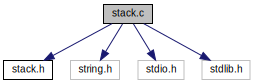
\includegraphics[width=326pt]{stack_8c__incl}
\end{center}
\end{figure}
\subsection*{Classes}
\begin{DoxyCompactItemize}
\item 
struct \hyperlink{structrecord}{record}
\begin{DoxyCompactList}\small\item\em Estrutura para o valor a armazenar. \end{DoxyCompactList}\item 
struct \hyperlink{structlista}{lista}
\begin{DoxyCompactList}\small\item\em Estrutura para a lista ligada. \end{DoxyCompactList}\item 
struct \hyperlink{structstack}{stack}
\begin{DoxyCompactList}\small\item\em Declaração da Estrutura principal. \end{DoxyCompactList}\end{DoxyCompactItemize}
\subsection*{Typedefs}
\begin{DoxyCompactItemize}
\item 
\hypertarget{stack_8c_a44e8f2943831641ea8ac9a833b65f08c}{typedef struct \hyperlink{structrecord}{record} \hyperlink{stack_8c_a44e8f2943831641ea8ac9a833b65f08c}{R\+E\+C\+O\+R\+D}}\label{stack_8c_a44e8f2943831641ea8ac9a833b65f08c}

\begin{DoxyCompactList}\small\item\em Estrutura para o valor a armazenar. \end{DoxyCompactList}\item 
\hypertarget{stack_8c_ab3843315393c74d2ade69877ac22d661}{typedef struct \hyperlink{structlista}{lista} $\ast$ \hyperlink{stack_8c_ab3843315393c74d2ade69877ac22d661}{L\+Rec}}\label{stack_8c_ab3843315393c74d2ade69877ac22d661}

\begin{DoxyCompactList}\small\item\em Estrutura para a lista ligada. \end{DoxyCompactList}\item 
\hypertarget{stack_8c_a4b4ce005aaf46d538cc28d07482e137e}{typedef struct \hyperlink{structstack}{stack} $\ast$ \hyperlink{stack_8c_a4b4ce005aaf46d538cc28d07482e137e}{S\+T\+A\+C\+K}}\label{stack_8c_a4b4ce005aaf46d538cc28d07482e137e}

\begin{DoxyCompactList}\small\item\em Declaração da Estrutura principal. \end{DoxyCompactList}\end{DoxyCompactItemize}
\subsection*{Functions}
\begin{DoxyCompactItemize}
\item 
\hyperlink{stack_8c_a4b4ce005aaf46d538cc28d07482e137e}{S\+T\+A\+C\+K} \hyperlink{stack_8c_ae737401bf8d705ce7fac339f553696bb}{init\+S} ()
\begin{DoxyCompactList}\small\item\em Cria uma instância destes módulo. \end{DoxyCompactList}\item 
void \hyperlink{stack_8c_ad57d238196f579aa8ad21efd9dedc734}{destroy\+S} (\hyperlink{stack_8c_a4b4ce005aaf46d538cc28d07482e137e}{S\+T\+A\+C\+K} s)
\begin{DoxyCompactList}\small\item\em Destrói uma instância destes módulo. \end{DoxyCompactList}\item 
int \hyperlink{stack_8c_aa2e25739a0ea0041423448bdcc5559c3}{is\+Empty} (\hyperlink{stack_8c_a4b4ce005aaf46d538cc28d07482e137e}{S\+T\+A\+C\+K} s)
\begin{DoxyCompactList}\small\item\em Verifica se a stack está vazia. \end{DoxyCompactList}\item 
void \hyperlink{stack_8c_a734636978e69eedc1efd53ddc858d360}{push} (\hyperlink{stack_8c_a4b4ce005aaf46d538cc28d07482e137e}{S\+T\+A\+C\+K} s, int i, int j, char val)
\begin{DoxyCompactList}\small\item\em Põe um elemento no topo da stack. \end{DoxyCompactList}\item 
int \hyperlink{stack_8c_aaf4563f073d541201c7601184039b879}{pop} (\hyperlink{stack_8c_a4b4ce005aaf46d538cc28d07482e137e}{S\+T\+A\+C\+K} s, int $\ast$i, int $\ast$j, char $\ast$flag)
\begin{DoxyCompactList}\small\item\em Tira um elemento no topo da stack. \end{DoxyCompactList}\item 
int \hyperlink{stack_8c_a105edf65b7e96281c133bee40d35ca9f}{peek} (\hyperlink{stack_8c_a4b4ce005aaf46d538cc28d07482e137e}{S\+T\+A\+C\+K} s)
\begin{DoxyCompactList}\small\item\em Consulta o elemento no topo da stack e alterar este para 0. \end{DoxyCompactList}\item 
int \hyperlink{stack_8c_a0cfa1c1680d521fb7da8a03b20c2b1f1}{can\+Get\+Anc} (\hyperlink{stack_8c_a4b4ce005aaf46d538cc28d07482e137e}{S\+T\+A\+C\+K} s)
\begin{DoxyCompactList}\small\item\em Verifica se a Stack possui uma âncora. \end{DoxyCompactList}\item 
int \hyperlink{stack_8c_a57784d722b977fd9dc3f17dfec32b7aa}{make\+Anc} (\hyperlink{stack_8c_a4b4ce005aaf46d538cc28d07482e137e}{S\+T\+A\+C\+K} s)
\begin{DoxyCompactList}\small\item\em Coloca, se possivél, uma âncora. \end{DoxyCompactList}\item 
char $\ast$ \hyperlink{stack_8c_ab9b9993c40e51034e26060048f6116e2}{complete\+S} (\hyperlink{stack_8c_a4b4ce005aaf46d538cc28d07482e137e}{S\+T\+A\+C\+K} s)
\begin{DoxyCompactList}\small\item\em Cria uma string correspondente aos elementos de uma {\ttfamily S\+T\+A\+C\+K} , aplicando {\ttfamily pop} a todos os elementos. \end{DoxyCompactList}\item 
void \hyperlink{stack_8c_a84b5260749650f26ce95bd755a43dde3}{add\+To\+Tail} (\hyperlink{stack_8c_a4b4ce005aaf46d538cc28d07482e137e}{S\+T\+A\+C\+K} s, char i, char j, char val, char check)
\begin{DoxyCompactList}\small\item\em Recebe um conjunto de valores e adiciona à cauda da lista em tempo constante. \end{DoxyCompactList}\end{DoxyCompactItemize}


\subsection{Detailed Description}
Módulo para operar sobre S\+T\+A\+C\+K. 



\subsection{Function Documentation}
\hypertarget{stack_8c_a84b5260749650f26ce95bd755a43dde3}{\index{stack.\+c@{stack.\+c}!add\+To\+Tail@{add\+To\+Tail}}
\index{add\+To\+Tail@{add\+To\+Tail}!stack.\+c@{stack.\+c}}
\subsubsection[{add\+To\+Tail}]{\setlength{\rightskip}{0pt plus 5cm}void add\+To\+Tail (
\begin{DoxyParamCaption}
\item[{{\bf S\+T\+A\+C\+K}}]{s, }
\item[{char}]{i, }
\item[{char}]{j, }
\item[{char}]{val, }
\item[{char}]{check}
\end{DoxyParamCaption}
)}}\label{stack_8c_a84b5260749650f26ce95bd755a43dde3}


Recebe um conjunto de valores e adiciona à cauda da lista em tempo constante. 


\begin{DoxyParams}{Parameters}
{\em s} & stack onde irá colocar o elemento. \\
\hline
{\em i} & Valor a adicionar. \\
\hline
{\em j} & Valor a adicionar. \\
\hline
{\em val} & Valor a adicionar. \\
\hline
{\em check} & Valor a adicionar. \\
\hline
\end{DoxyParams}
\hypertarget{stack_8c_a0cfa1c1680d521fb7da8a03b20c2b1f1}{\index{stack.\+c@{stack.\+c}!can\+Get\+Anc@{can\+Get\+Anc}}
\index{can\+Get\+Anc@{can\+Get\+Anc}!stack.\+c@{stack.\+c}}
\subsubsection[{can\+Get\+Anc}]{\setlength{\rightskip}{0pt plus 5cm}int can\+Get\+Anc (
\begin{DoxyParamCaption}
\item[{{\bf S\+T\+A\+C\+K}}]{s}
\end{DoxyParamCaption}
)}}\label{stack_8c_a0cfa1c1680d521fb7da8a03b20c2b1f1}


Verifica se a Stack possui uma âncora. 


\begin{DoxyParams}{Parameters}
{\em s} & Instância de Stack que se pertende consultar\\
\hline
\end{DoxyParams}
\begin{DoxyReturn}{Returns}
Devolve 1 se existir uma âncora na {\ttfamily S\+T\+A\+C\+K}, 0 caso contrário.
\end{DoxyReturn}
\begin{DoxySeeAlso}{See also}
\hyperlink{structrecord_a381a80a513768c3eba6b765c5e356bad}{record\+::check} 
\end{DoxySeeAlso}
\hypertarget{stack_8c_ab9b9993c40e51034e26060048f6116e2}{\index{stack.\+c@{stack.\+c}!complete\+S@{complete\+S}}
\index{complete\+S@{complete\+S}!stack.\+c@{stack.\+c}}
\subsubsection[{complete\+S}]{\setlength{\rightskip}{0pt plus 5cm}char $\ast$ complete\+S (
\begin{DoxyParamCaption}
\item[{{\bf S\+T\+A\+C\+K}}]{s}
\end{DoxyParamCaption}
)}}\label{stack_8c_ab9b9993c40e51034e26060048f6116e2}


Cria uma string correspondente aos elementos de uma {\ttfamily S\+T\+A\+C\+K} , aplicando {\ttfamily pop} a todos os elementos. 


\begin{DoxyParams}{Parameters}
{\em s} & A {\ttfamily S\+T\+A\+C\+K} que irá passar a string.\\
\hline
\end{DoxyParams}
\begin{DoxyReturn}{Returns}
A string correspondente à {\ttfamily S\+T\+A\+C\+K} .
\end{DoxyReturn}
\begin{DoxySeeAlso}{See also}
\hyperlink{stack_8c_aaf4563f073d541201c7601184039b879}{pop} 
\end{DoxySeeAlso}
\hypertarget{stack_8c_ad57d238196f579aa8ad21efd9dedc734}{\index{stack.\+c@{stack.\+c}!destroy\+S@{destroy\+S}}
\index{destroy\+S@{destroy\+S}!stack.\+c@{stack.\+c}}
\subsubsection[{destroy\+S}]{\setlength{\rightskip}{0pt plus 5cm}void destroy\+S (
\begin{DoxyParamCaption}
\item[{{\bf S\+T\+A\+C\+K}}]{s}
\end{DoxyParamCaption}
)}}\label{stack_8c_ad57d238196f579aa8ad21efd9dedc734}


Destrói uma instância destes módulo. 


\begin{DoxyParams}{Parameters}
{\em s} & Instância de Stack a ser destruida. \\
\hline
\end{DoxyParams}
\hypertarget{stack_8c_ae737401bf8d705ce7fac339f553696bb}{\index{stack.\+c@{stack.\+c}!init\+S@{init\+S}}
\index{init\+S@{init\+S}!stack.\+c@{stack.\+c}}
\subsubsection[{init\+S}]{\setlength{\rightskip}{0pt plus 5cm}{\bf S\+T\+A\+C\+K} init\+S (
\begin{DoxyParamCaption}
{}
\end{DoxyParamCaption}
)}}\label{stack_8c_ae737401bf8d705ce7fac339f553696bb}


Cria uma instância destes módulo. 

\begin{DoxyReturn}{Returns}
{\ttfamily S\+T\+A\+C\+K} criada. 
\end{DoxyReturn}
\hypertarget{stack_8c_aa2e25739a0ea0041423448bdcc5559c3}{\index{stack.\+c@{stack.\+c}!is\+Empty@{is\+Empty}}
\index{is\+Empty@{is\+Empty}!stack.\+c@{stack.\+c}}
\subsubsection[{is\+Empty}]{\setlength{\rightskip}{0pt plus 5cm}int is\+Empty (
\begin{DoxyParamCaption}
\item[{{\bf S\+T\+A\+C\+K}}]{s}
\end{DoxyParamCaption}
)}}\label{stack_8c_aa2e25739a0ea0041423448bdcc5559c3}


Verifica se a stack está vazia. 


\begin{DoxyParams}{Parameters}
{\em s} & Instância de Stack que se pertender verificar se está vazia. \\
\hline
\end{DoxyParams}
\hypertarget{stack_8c_a57784d722b977fd9dc3f17dfec32b7aa}{\index{stack.\+c@{stack.\+c}!make\+Anc@{make\+Anc}}
\index{make\+Anc@{make\+Anc}!stack.\+c@{stack.\+c}}
\subsubsection[{make\+Anc}]{\setlength{\rightskip}{0pt plus 5cm}int make\+Anc (
\begin{DoxyParamCaption}
\item[{{\bf S\+T\+A\+C\+K}}]{s}
\end{DoxyParamCaption}
)}}\label{stack_8c_a57784d722b977fd9dc3f17dfec32b7aa}


Coloca, se possivél, uma âncora. 


\begin{DoxyParams}{Parameters}
{\em s} & A stack que onde irá ser guardada a âncora.\\
\hline
\end{DoxyParams}
\begin{DoxyReturn}{Returns}
Devolve 1 se foi possivél colocar uma âncora, 0 caso contrário.
\end{DoxyReturn}
\begin{DoxySeeAlso}{See also}
\hyperlink{structrecord_a381a80a513768c3eba6b765c5e356bad}{record\+::check} 
\end{DoxySeeAlso}
\hypertarget{stack_8c_a105edf65b7e96281c133bee40d35ca9f}{\index{stack.\+c@{stack.\+c}!peek@{peek}}
\index{peek@{peek}!stack.\+c@{stack.\+c}}
\subsubsection[{peek}]{\setlength{\rightskip}{0pt plus 5cm}int peek (
\begin{DoxyParamCaption}
\item[{{\bf S\+T\+A\+C\+K}}]{s}
\end{DoxyParamCaption}
)}}\label{stack_8c_a105edf65b7e96281c133bee40d35ca9f}


Consulta o elemento no topo da stack e alterar este para 0. 


\begin{DoxyParams}{Parameters}
{\em s} & Instância de Stack que se pertende consultar\\
\hline
\end{DoxyParams}
\begin{DoxyReturn}{Returns}
{\bfseries -\/1} se a {\ttfamily S\+T\+A\+C\+K} for vazia, caso contrário devolve o valor indicativo de âncora no topo da {\ttfamily S\+T\+A\+C\+K} .
\end{DoxyReturn}
\begin{DoxySeeAlso}{See also}
\hyperlink{structrecord_a381a80a513768c3eba6b765c5e356bad}{record\+::check} 
\end{DoxySeeAlso}
\hypertarget{stack_8c_aaf4563f073d541201c7601184039b879}{\index{stack.\+c@{stack.\+c}!pop@{pop}}
\index{pop@{pop}!stack.\+c@{stack.\+c}}
\subsubsection[{pop}]{\setlength{\rightskip}{0pt plus 5cm}int pop (
\begin{DoxyParamCaption}
\item[{{\bf S\+T\+A\+C\+K}}]{s, }
\item[{int $\ast$}]{i, }
\item[{int $\ast$}]{j, }
\item[{char $\ast$}]{flag}
\end{DoxyParamCaption}
)}}\label{stack_8c_aaf4563f073d541201c7601184039b879}


Tira um elemento no topo da stack. 


\begin{DoxyParams}{Parameters}
{\em s} & Instância de Stack que se pertende remover uma entrada. \\
\hline
{\em i} & abcissas do elemento que se retirou. \\
\hline
{\em j} & ordenada do elemento que se retirou. \\
\hline
{\em flag} & valor a guardar.\\
\hline
\end{DoxyParams}
\begin{DoxyReturn}{Returns}
{\bfseries -\/1} se a {\ttfamily S\+T\+A\+C\+K} for vazia, caso contrário retorna o valor retirado.
\end{DoxyReturn}
\begin{DoxySeeAlso}{See also}
\hyperlink{structrecord_a125d17b59037591de0a682688802f670}{record\+::val} 
\end{DoxySeeAlso}
\hypertarget{stack_8c_a734636978e69eedc1efd53ddc858d360}{\index{stack.\+c@{stack.\+c}!push@{push}}
\index{push@{push}!stack.\+c@{stack.\+c}}
\subsubsection[{push}]{\setlength{\rightskip}{0pt plus 5cm}void push (
\begin{DoxyParamCaption}
\item[{{\bf S\+T\+A\+C\+K}}]{s, }
\item[{int}]{i, }
\item[{int}]{j, }
\item[{char}]{val}
\end{DoxyParamCaption}
)}}\label{stack_8c_a734636978e69eedc1efd53ddc858d360}


Põe um elemento no topo da stack. 


\begin{DoxyParams}{Parameters}
{\em s} & Instância de Stack que se pertende adicionar uma entrada. \\
\hline
{\em i} & abcissas do elemento a guardar. \\
\hline
{\em j} & ordenada do elemento a guardar. \\
\hline
{\em val} & valor a guardar. \\
\hline
\end{DoxyParams}

\hypertarget{stack_8h}{\section{stack.\+h File Reference}
\label{stack_8h}\index{stack.\+h@{stack.\+h}}
}


Módulo para operar sobre S\+T\+A\+C\+K.  


This graph shows which files directly or indirectly include this file\+:
\nopagebreak
\begin{figure}[H]
\begin{center}
\leavevmode
\includegraphics[width=350pt]{stack_8h__dep__incl}
\end{center}
\end{figure}
\subsection*{Typedefs}
\begin{DoxyCompactItemize}
\item 
\hypertarget{stack_8h_a96c29a043be1d5a749a2452809ba9b8d}{typedef struct \hyperlink{structstack}{stack} $\ast$ \hyperlink{stack_8h_a96c29a043be1d5a749a2452809ba9b8d}{S\+T\+A\+C\+K}}\label{stack_8h_a96c29a043be1d5a749a2452809ba9b8d}

\begin{DoxyCompactList}\small\item\em Declaração da Estrutura principal. \end{DoxyCompactList}\end{DoxyCompactItemize}
\subsection*{Functions}
\begin{DoxyCompactItemize}
\item 
\hyperlink{stack_8c_a4b4ce005aaf46d538cc28d07482e137e}{S\+T\+A\+C\+K} \hyperlink{stack_8h_ae737401bf8d705ce7fac339f553696bb}{init\+S} ()
\begin{DoxyCompactList}\small\item\em Cria uma instância destes módulo. \end{DoxyCompactList}\item 
void \hyperlink{stack_8h_ad57d238196f579aa8ad21efd9dedc734}{destroy\+S} (\hyperlink{stack_8c_a4b4ce005aaf46d538cc28d07482e137e}{S\+T\+A\+C\+K} s)
\begin{DoxyCompactList}\small\item\em Destrói uma instância destes módulo. \end{DoxyCompactList}\item 
int \hyperlink{stack_8h_aa2e25739a0ea0041423448bdcc5559c3}{is\+Empty} (\hyperlink{stack_8c_a4b4ce005aaf46d538cc28d07482e137e}{S\+T\+A\+C\+K} s)
\begin{DoxyCompactList}\small\item\em Verifica se a stack está vazia. \end{DoxyCompactList}\item 
void \hyperlink{stack_8h_a734636978e69eedc1efd53ddc858d360}{push} (\hyperlink{stack_8c_a4b4ce005aaf46d538cc28d07482e137e}{S\+T\+A\+C\+K} s, int i, int j, char val)
\begin{DoxyCompactList}\small\item\em Põe um elemento no topo da stack. \end{DoxyCompactList}\item 
int \hyperlink{stack_8h_aaf4563f073d541201c7601184039b879}{pop} (\hyperlink{stack_8c_a4b4ce005aaf46d538cc28d07482e137e}{S\+T\+A\+C\+K} s, int $\ast$i, int $\ast$j, char $\ast$flag)
\begin{DoxyCompactList}\small\item\em Tira um elemento no topo da stack. \end{DoxyCompactList}\item 
int \hyperlink{stack_8h_a105edf65b7e96281c133bee40d35ca9f}{peek} (\hyperlink{stack_8c_a4b4ce005aaf46d538cc28d07482e137e}{S\+T\+A\+C\+K} s)
\begin{DoxyCompactList}\small\item\em Consulta o elemento no topo da stack e alterar este para 0. \end{DoxyCompactList}\item 
int \hyperlink{stack_8h_a0cfa1c1680d521fb7da8a03b20c2b1f1}{can\+Get\+Anc} (\hyperlink{stack_8c_a4b4ce005aaf46d538cc28d07482e137e}{S\+T\+A\+C\+K} s)
\begin{DoxyCompactList}\small\item\em Verifica se a Stack possui uma âncora. \end{DoxyCompactList}\item 
int \hyperlink{stack_8h_a57784d722b977fd9dc3f17dfec32b7aa}{make\+Anc} (\hyperlink{stack_8c_a4b4ce005aaf46d538cc28d07482e137e}{S\+T\+A\+C\+K} s)
\begin{DoxyCompactList}\small\item\em Coloca, se possivél, uma âncora. \end{DoxyCompactList}\item 
void \hyperlink{stack_8h_a84b5260749650f26ce95bd755a43dde3}{add\+To\+Tail} (\hyperlink{stack_8c_a4b4ce005aaf46d538cc28d07482e137e}{S\+T\+A\+C\+K} s, char i, char j, char val, char check)
\begin{DoxyCompactList}\small\item\em Recebe um conjunto de valores e adiciona à cauda da lista em tempo constante. \end{DoxyCompactList}\item 
char $\ast$ \hyperlink{stack_8h_aae137601ef0f93e72af0c0c05b3266e5}{complete\+S} (\hyperlink{stack_8c_a4b4ce005aaf46d538cc28d07482e137e}{S\+T\+A\+C\+K} s)
\begin{DoxyCompactList}\small\item\em Cria uma string correspondente aos elementos de uma {\ttfamily S\+T\+A\+C\+K} , aplicando {\ttfamily pop} a todos os elementos. \end{DoxyCompactList}\end{DoxyCompactItemize}


\subsection{Detailed Description}
Módulo para operar sobre S\+T\+A\+C\+K. 



\subsection{Function Documentation}
\hypertarget{stack_8h_a84b5260749650f26ce95bd755a43dde3}{\index{stack.\+h@{stack.\+h}!add\+To\+Tail@{add\+To\+Tail}}
\index{add\+To\+Tail@{add\+To\+Tail}!stack.\+h@{stack.\+h}}
\subsubsection[{add\+To\+Tail}]{\setlength{\rightskip}{0pt plus 5cm}void add\+To\+Tail (
\begin{DoxyParamCaption}
\item[{{\bf S\+T\+A\+C\+K}}]{s, }
\item[{char}]{i, }
\item[{char}]{j, }
\item[{char}]{val, }
\item[{char}]{check}
\end{DoxyParamCaption}
)}}\label{stack_8h_a84b5260749650f26ce95bd755a43dde3}


Recebe um conjunto de valores e adiciona à cauda da lista em tempo constante. 


\begin{DoxyParams}{Parameters}
{\em s} & stack onde irá colocar o elemento. \\
\hline
{\em i} & Valor a adicionar. \\
\hline
{\em j} & Valor a adicionar. \\
\hline
{\em val} & Valor a adicionar. \\
\hline
{\em check} & Valor a adicionar. \\
\hline
\end{DoxyParams}
\hypertarget{stack_8h_a0cfa1c1680d521fb7da8a03b20c2b1f1}{\index{stack.\+h@{stack.\+h}!can\+Get\+Anc@{can\+Get\+Anc}}
\index{can\+Get\+Anc@{can\+Get\+Anc}!stack.\+h@{stack.\+h}}
\subsubsection[{can\+Get\+Anc}]{\setlength{\rightskip}{0pt plus 5cm}int can\+Get\+Anc (
\begin{DoxyParamCaption}
\item[{{\bf S\+T\+A\+C\+K}}]{s}
\end{DoxyParamCaption}
)}}\label{stack_8h_a0cfa1c1680d521fb7da8a03b20c2b1f1}


Verifica se a Stack possui uma âncora. 


\begin{DoxyParams}{Parameters}
{\em s} & Instância de Stack que se pertende consultar\\
\hline
\end{DoxyParams}
\begin{DoxyReturn}{Returns}
Devolve 1 se existir uma âncora na {\ttfamily S\+T\+A\+C\+K}, 0 caso contrário.
\end{DoxyReturn}
\begin{DoxySeeAlso}{See also}
\hyperlink{structrecord_a381a80a513768c3eba6b765c5e356bad}{record\+::check} 
\end{DoxySeeAlso}
\hypertarget{stack_8h_aae137601ef0f93e72af0c0c05b3266e5}{\index{stack.\+h@{stack.\+h}!complete\+S@{complete\+S}}
\index{complete\+S@{complete\+S}!stack.\+h@{stack.\+h}}
\subsubsection[{complete\+S}]{\setlength{\rightskip}{0pt plus 5cm}char$\ast$ complete\+S (
\begin{DoxyParamCaption}
\item[{{\bf S\+T\+A\+C\+K}}]{s}
\end{DoxyParamCaption}
)}}\label{stack_8h_aae137601ef0f93e72af0c0c05b3266e5}


Cria uma string correspondente aos elementos de uma {\ttfamily S\+T\+A\+C\+K} , aplicando {\ttfamily pop} a todos os elementos. 


\begin{DoxyParams}{Parameters}
{\em s} & A {\ttfamily S\+T\+A\+C\+K} que irá passar a string.\\
\hline
\end{DoxyParams}
\begin{DoxyReturn}{Returns}
A string correspondente à {\ttfamily S\+T\+A\+C\+K} .
\end{DoxyReturn}
\begin{DoxySeeAlso}{See also}
\hyperlink{stack_8c_aaf4563f073d541201c7601184039b879}{pop} 
\end{DoxySeeAlso}
\hypertarget{stack_8h_ad57d238196f579aa8ad21efd9dedc734}{\index{stack.\+h@{stack.\+h}!destroy\+S@{destroy\+S}}
\index{destroy\+S@{destroy\+S}!stack.\+h@{stack.\+h}}
\subsubsection[{destroy\+S}]{\setlength{\rightskip}{0pt plus 5cm}void destroy\+S (
\begin{DoxyParamCaption}
\item[{{\bf S\+T\+A\+C\+K}}]{s}
\end{DoxyParamCaption}
)}}\label{stack_8h_ad57d238196f579aa8ad21efd9dedc734}


Destrói uma instância destes módulo. 


\begin{DoxyParams}{Parameters}
{\em s} & Instância de Stack a ser destruida. \\
\hline
\end{DoxyParams}
\hypertarget{stack_8h_ae737401bf8d705ce7fac339f553696bb}{\index{stack.\+h@{stack.\+h}!init\+S@{init\+S}}
\index{init\+S@{init\+S}!stack.\+h@{stack.\+h}}
\subsubsection[{init\+S}]{\setlength{\rightskip}{0pt plus 5cm}{\bf S\+T\+A\+C\+K} init\+S (
\begin{DoxyParamCaption}
{}
\end{DoxyParamCaption}
)}}\label{stack_8h_ae737401bf8d705ce7fac339f553696bb}


Cria uma instância destes módulo. 

\begin{DoxyReturn}{Returns}
{\ttfamily S\+T\+A\+C\+K} criada. 
\end{DoxyReturn}
\hypertarget{stack_8h_aa2e25739a0ea0041423448bdcc5559c3}{\index{stack.\+h@{stack.\+h}!is\+Empty@{is\+Empty}}
\index{is\+Empty@{is\+Empty}!stack.\+h@{stack.\+h}}
\subsubsection[{is\+Empty}]{\setlength{\rightskip}{0pt plus 5cm}int is\+Empty (
\begin{DoxyParamCaption}
\item[{{\bf S\+T\+A\+C\+K}}]{s}
\end{DoxyParamCaption}
)}}\label{stack_8h_aa2e25739a0ea0041423448bdcc5559c3}


Verifica se a stack está vazia. 


\begin{DoxyParams}{Parameters}
{\em s} & Instância de Stack que se pertender verificar se está vazia. \\
\hline
\end{DoxyParams}
\hypertarget{stack_8h_a57784d722b977fd9dc3f17dfec32b7aa}{\index{stack.\+h@{stack.\+h}!make\+Anc@{make\+Anc}}
\index{make\+Anc@{make\+Anc}!stack.\+h@{stack.\+h}}
\subsubsection[{make\+Anc}]{\setlength{\rightskip}{0pt plus 5cm}int make\+Anc (
\begin{DoxyParamCaption}
\item[{{\bf S\+T\+A\+C\+K}}]{s}
\end{DoxyParamCaption}
)}}\label{stack_8h_a57784d722b977fd9dc3f17dfec32b7aa}


Coloca, se possivél, uma âncora. 


\begin{DoxyParams}{Parameters}
{\em s} & A stack que onde irá ser guardada a âncora.\\
\hline
\end{DoxyParams}
\begin{DoxyReturn}{Returns}
Devolve 1 se foi possivél colocar uma âncora, 0 caso contrário.
\end{DoxyReturn}
\begin{DoxySeeAlso}{See also}
\hyperlink{structrecord_a381a80a513768c3eba6b765c5e356bad}{record\+::check} 
\end{DoxySeeAlso}
\hypertarget{stack_8h_a105edf65b7e96281c133bee40d35ca9f}{\index{stack.\+h@{stack.\+h}!peek@{peek}}
\index{peek@{peek}!stack.\+h@{stack.\+h}}
\subsubsection[{peek}]{\setlength{\rightskip}{0pt plus 5cm}int peek (
\begin{DoxyParamCaption}
\item[{{\bf S\+T\+A\+C\+K}}]{s}
\end{DoxyParamCaption}
)}}\label{stack_8h_a105edf65b7e96281c133bee40d35ca9f}


Consulta o elemento no topo da stack e alterar este para 0. 


\begin{DoxyParams}{Parameters}
{\em s} & Instância de Stack que se pertende consultar\\
\hline
\end{DoxyParams}
\begin{DoxyReturn}{Returns}
{\bfseries -\/1} se a {\ttfamily S\+T\+A\+C\+K} for vazia, caso contrário devolve o valor indicativo de âncora no topo da {\ttfamily S\+T\+A\+C\+K} .
\end{DoxyReturn}
\begin{DoxySeeAlso}{See also}
\hyperlink{structrecord_a381a80a513768c3eba6b765c5e356bad}{record\+::check} 
\end{DoxySeeAlso}
\hypertarget{stack_8h_aaf4563f073d541201c7601184039b879}{\index{stack.\+h@{stack.\+h}!pop@{pop}}
\index{pop@{pop}!stack.\+h@{stack.\+h}}
\subsubsection[{pop}]{\setlength{\rightskip}{0pt plus 5cm}int pop (
\begin{DoxyParamCaption}
\item[{{\bf S\+T\+A\+C\+K}}]{s, }
\item[{int $\ast$}]{i, }
\item[{int $\ast$}]{j, }
\item[{char $\ast$}]{flag}
\end{DoxyParamCaption}
)}}\label{stack_8h_aaf4563f073d541201c7601184039b879}


Tira um elemento no topo da stack. 


\begin{DoxyParams}{Parameters}
{\em s} & Instância de Stack que se pertende remover uma entrada. \\
\hline
{\em i} & abcissas do elemento que se retirou. \\
\hline
{\em j} & ordenada do elemento que se retirou. \\
\hline
{\em flag} & valor a guardar.\\
\hline
\end{DoxyParams}
\begin{DoxyReturn}{Returns}
{\bfseries -\/1} se a {\ttfamily S\+T\+A\+C\+K} for vazia, caso contrário retorna o valor retirado.
\end{DoxyReturn}
\begin{DoxySeeAlso}{See also}
\hyperlink{structrecord_a125d17b59037591de0a682688802f670}{record\+::val} 
\end{DoxySeeAlso}
\hypertarget{stack_8h_a734636978e69eedc1efd53ddc858d360}{\index{stack.\+h@{stack.\+h}!push@{push}}
\index{push@{push}!stack.\+h@{stack.\+h}}
\subsubsection[{push}]{\setlength{\rightskip}{0pt plus 5cm}void push (
\begin{DoxyParamCaption}
\item[{{\bf S\+T\+A\+C\+K}}]{s, }
\item[{int}]{i, }
\item[{int}]{j, }
\item[{char}]{val}
\end{DoxyParamCaption}
)}}\label{stack_8h_a734636978e69eedc1efd53ddc858d360}


Põe um elemento no topo da stack. 


\begin{DoxyParams}{Parameters}
{\em s} & Instância de Stack que se pertende adicionar uma entrada. \\
\hline
{\em i} & abcissas do elemento a guardar. \\
\hline
{\em j} & ordenada do elemento a guardar. \\
\hline
{\em val} & valor a guardar. \\
\hline
\end{DoxyParams}

\hypertarget{state_8c}{\section{state.\+c File Reference}
\label{state_8c}\index{state.\+c@{state.\+c}}
}


Módulo para alterar estado.  


{\ttfamily \#include \char`\"{}estado.\+h\char`\"{}}\\*
{\ttfamily \#include \char`\"{}state.\+h\char`\"{}}\\*
{\ttfamily \#include \char`\"{}decide.\+h\char`\"{}}\\*
{\ttfamily \#include \char`\"{}stack.\+h\char`\"{}}\\*
{\ttfamily \#include \char`\"{}filemanager.\+h\char`\"{}}\\*
{\ttfamily \#include \char`\"{}solver.\+h\char`\"{}}\\*
{\ttfamily \#include \char`\"{}frontend.\+h\char`\"{}}\\*
{\ttfamily \#include \char`\"{}validate.\+h\char`\"{}}\\*
{\ttfamily \#include $<$string.\+h$>$}\\*
Include dependency graph for state.\+c\+:
\nopagebreak
\begin{figure}[H]
\begin{center}
\leavevmode
\includegraphics[width=350pt]{state_8c__incl}
\end{center}
\end{figure}
\subsection*{Macros}
\begin{DoxyCompactItemize}
\item 
\#define \hyperlink{state_8c_ae024ee88ce892fab4a83ea2be5185cfa}{limit}(num)~((num $>$ 0) \&\& (num $<$ \hyperlink{estado_8h_ab02e1c5c6948bf8cf3c21a0acad8a578}{M\+A\+X\+\_\+\+G\+R\+I\+D}))
\begin{DoxyCompactList}\small\item\em Macro que verifica se o 'num' se encontra nos limites indicados. \end{DoxyCompactList}\item 
\#define \hyperlink{state_8c_acbc8990e81e4a745cbb34fe695ae9788}{extracase}(num, vec)~( (num == \hyperlink{estado_8h_ab02e1c5c6948bf8cf3c21a0acad8a578}{M\+A\+X\+\_\+\+G\+R\+I\+D} \&\& vec $<$ 0))
\begin{DoxyCompactList}\small\item\em Macro que verifica se 'num' e 'vec' se encontram no caso especifico indicado. \end{DoxyCompactList}\end{DoxyCompactItemize}
\subsection*{Functions}
\begin{DoxyCompactItemize}
\item 
void \hyperlink{state_8c_a11aed0a30a94f6dbf787a6c73dbd6409}{clearstate} (\hyperlink{estado_8c_afbffb4e9c242f93d5a2d607754ce2db8}{E\+S\+T\+A\+D\+O} e)
\begin{DoxyCompactList}\small\item\em Função que converte para vazia todas as peças não fixas. \end{DoxyCompactList}\item 
void \hyperlink{state_8c_a8f967d9da54fb07016a74353f7a230ee}{clearcanvas} (\hyperlink{estado_8c_afbffb4e9c242f93d5a2d607754ce2db8}{E\+S\+T\+A\+D\+O} e)
\begin{DoxyCompactList}\small\item\em Função que converte todas as peças para vazia. \end{DoxyCompactList}\item 
void \hyperlink{state_8c_a1775e9c25dcb0dcf9d03020f281c4ca8}{makefixo} (\hyperlink{estado_8c_afbffb4e9c242f93d5a2d607754ce2db8}{E\+S\+T\+A\+D\+O} e)
\begin{DoxyCompactList}\small\item\em Função que converte todas as peças soltas para fixas. \end{DoxyCompactList}\item 
void \hyperlink{state_8c_a1bee768ce8693d3a440b5a60b545dce3}{increase} (\hyperlink{estado_8c_afbffb4e9c242f93d5a2d607754ce2db8}{E\+S\+T\+A\+D\+O} e, int ox, int oy)
\begin{DoxyCompactList}\small\item\em Função que incrementa o tamanho de um tabuleiro. \end{DoxyCompactList}\item 
void \hyperlink{state_8c_abcfe0e950583a81bc2a7586eb7d044b5}{safedraw} (\hyperlink{estado_8c_afbffb4e9c242f93d5a2d607754ce2db8}{E\+S\+T\+A\+D\+O} e)
\begin{DoxyCompactList}\small\item\em Função que converte todas as peças para fixo e muda para o menu de Jogar. \end{DoxyCompactList}\item 
int \hyperlink{state_8c_a326d958585b69c8ea98488815583cfaf}{victory} (\hyperlink{estado_8c_afbffb4e9c242f93d5a2d607754ce2db8}{E\+S\+T\+A\+D\+O} e)
\begin{DoxyCompactList}\small\item\em Função que verifica se o tabuleiro não tem peças vazias. \end{DoxyCompactList}\item 
int \hyperlink{state_8c_a695e69034d7f22ba4eb4489af2e8786c}{save\+Anc} (\hyperlink{estado_8c_afbffb4e9c242f93d5a2d607754ce2db8}{E\+S\+T\+A\+D\+O} e)
\begin{DoxyCompactList}\small\item\em Função que guarda uma âncora. \end{DoxyCompactList}\item 
void \hyperlink{state_8c_aa72d6a8965f5d7a3d214a4ecde14ecc0}{pop\+\_\+\+Anc} (\hyperlink{estado_8c_afbffb4e9c242f93d5a2d607754ce2db8}{E\+S\+T\+A\+D\+O} e)
\begin{DoxyCompactList}\small\item\em Função que carrega a última âncora. \end{DoxyCompactList}\item 
int \hyperlink{state_8c_affd00f2e02da4d53ecb069aeb0d5ce4b}{valid\+Tab} (\hyperlink{estado_8c_afbffb4e9c242f93d5a2d607754ce2db8}{E\+S\+T\+A\+D\+O} e)
\begin{DoxyCompactList}\small\item\em Verifica se um tabuleiro é válido. \end{DoxyCompactList}\item 
static char \hyperlink{state_8c_a2548e60a79422e129c9ec17075f76960}{cleansolto} (char val)
\begin{DoxyCompactList}\small\item\em Função que recebe uma peça e verifica se ela é solta. \end{DoxyCompactList}\item 
static char \hyperlink{state_8c_aa9cddc4fa064e7f8c404c4f055785590}{fixatepec} (char val)
\begin{DoxyCompactList}\small\item\em Função transforma uma peça na sua contraparte {\bfseries F\+I\+X\+A} . \end{DoxyCompactList}\item 
void \hyperlink{state_8c_ab9caafc0116aeec18705eda9533f132f}{pipestack} (\hyperlink{estado_8c_afbffb4e9c242f93d5a2d607754ce2db8}{E\+S\+T\+A\+D\+O} e, int c)
\begin{DoxyCompactList}\small\item\em Função que transfere um elemento entre as stacks do estado. \end{DoxyCompactList}\item 
int \hyperlink{state_8c_a9aebac26301ed491854416fbd9683ba8}{is\+\_\+not\+\_\+solto} (\hyperlink{estado_8c_afbffb4e9c242f93d5a2d607754ce2db8}{E\+S\+T\+A\+D\+O} e, int i, int j)
\begin{DoxyCompactList}\small\item\em Verifica se a peça dada não é vazia. \end{DoxyCompactList}\end{DoxyCompactItemize}


\subsection{Detailed Description}
Módulo para alterar estado. 



\subsection{Macro Definition Documentation}
\hypertarget{state_8c_acbc8990e81e4a745cbb34fe695ae9788}{\index{state.\+c@{state.\+c}!extracase@{extracase}}
\index{extracase@{extracase}!state.\+c@{state.\+c}}
\subsubsection[{extracase}]{\setlength{\rightskip}{0pt plus 5cm}\#define extracase(
\begin{DoxyParamCaption}
\item[{}]{num, }
\item[{}]{vec}
\end{DoxyParamCaption}
)~( (num == {\bf M\+A\+X\+\_\+\+G\+R\+I\+D} \&\& vec $<$ 0))}}\label{state_8c_acbc8990e81e4a745cbb34fe695ae9788}


Macro que verifica se 'num' e 'vec' se encontram no caso especifico indicado. 


\begin{DoxyParams}{Parameters}
{\em num} & Valor a comparar. \\
\hline
{\em vec} & Valor a comparar.\\
\hline
\end{DoxyParams}
\begin{DoxyReturn}{Returns}
devolve 1 se os valores se encontrarem no estado indicado, devolve 0 caso contrário. 
\end{DoxyReturn}
\hypertarget{state_8c_ae024ee88ce892fab4a83ea2be5185cfa}{\index{state.\+c@{state.\+c}!limit@{limit}}
\index{limit@{limit}!state.\+c@{state.\+c}}
\subsubsection[{limit}]{\setlength{\rightskip}{0pt plus 5cm}\#define limit(
\begin{DoxyParamCaption}
\item[{}]{num}
\end{DoxyParamCaption}
)~((num $>$ 0) \&\& (num $<$ {\bf M\+A\+X\+\_\+\+G\+R\+I\+D}))}}\label{state_8c_ae024ee88ce892fab4a83ea2be5185cfa}


Macro que verifica se o 'num' se encontra nos limites indicados. 


\begin{DoxyParams}{Parameters}
{\em num} & Valor a comparar.\\
\hline
\end{DoxyParams}
\begin{DoxyReturn}{Returns}
devolve 1 se o valor se encontrar entre 0 e M\+A\+X\+\_\+\+G\+R\+I\+D, devolve 0 caso contrário. 
\end{DoxyReturn}


\subsection{Function Documentation}
\hypertarget{state_8c_a2548e60a79422e129c9ec17075f76960}{\index{state.\+c@{state.\+c}!cleansolto@{cleansolto}}
\index{cleansolto@{cleansolto}!state.\+c@{state.\+c}}
\subsubsection[{cleansolto}]{\setlength{\rightskip}{0pt plus 5cm}static char cleansolto (
\begin{DoxyParamCaption}
\item[{char}]{val}
\end{DoxyParamCaption}
)\hspace{0.3cm}{\ttfamily [static]}}}\label{state_8c_a2548e60a79422e129c9ec17075f76960}


Função que recebe uma peça e verifica se ela é solta. 


\begin{DoxyParams}{Parameters}
{\em val} & Peça a verificar.\\
\hline
\end{DoxyParams}
\begin{DoxyReturn}{Returns}
Se val for S\+O\+L devolve V\+A\+Z\+I\+A, caso contrário devolve val. 
\end{DoxyReturn}
\hypertarget{state_8c_a8f967d9da54fb07016a74353f7a230ee}{\index{state.\+c@{state.\+c}!clearcanvas@{clearcanvas}}
\index{clearcanvas@{clearcanvas}!state.\+c@{state.\+c}}
\subsubsection[{clearcanvas}]{\setlength{\rightskip}{0pt plus 5cm}void clearcanvas (
\begin{DoxyParamCaption}
\item[{{\bf E\+S\+T\+A\+D\+O}}]{e}
\end{DoxyParamCaption}
)}}\label{state_8c_a8f967d9da54fb07016a74353f7a230ee}


Função que converte todas as peças para vazia. 


\begin{DoxyParams}{Parameters}
{\em e} & Estado a limpar.\\
\hline
\end{DoxyParams}
\begin{DoxySeeAlso}{See also}
\hyperlink{estado_8h_a5eff026b884b0da81f84f8658a3d850d}{set\+E\+\_\+base} 
\end{DoxySeeAlso}
\hypertarget{state_8c_a11aed0a30a94f6dbf787a6c73dbd6409}{\index{state.\+c@{state.\+c}!clearstate@{clearstate}}
\index{clearstate@{clearstate}!state.\+c@{state.\+c}}
\subsubsection[{clearstate}]{\setlength{\rightskip}{0pt plus 5cm}void clearstate (
\begin{DoxyParamCaption}
\item[{{\bf E\+S\+T\+A\+D\+O}}]{e}
\end{DoxyParamCaption}
)}}\label{state_8c_a11aed0a30a94f6dbf787a6c73dbd6409}


Função que converte para vazia todas as peças não fixas. 


\begin{DoxyParams}{Parameters}
{\em e} & Estado a limpar. \\
\hline
\end{DoxyParams}
\hypertarget{state_8c_aa9cddc4fa064e7f8c404c4f055785590}{\index{state.\+c@{state.\+c}!fixatepec@{fixatepec}}
\index{fixatepec@{fixatepec}!state.\+c@{state.\+c}}
\subsubsection[{fixatepec}]{\setlength{\rightskip}{0pt plus 5cm}static char fixatepec (
\begin{DoxyParamCaption}
\item[{char}]{val}
\end{DoxyParamCaption}
)\hspace{0.3cm}{\ttfamily [static]}}}\label{state_8c_aa9cddc4fa064e7f8c404c4f055785590}


Função transforma uma peça na sua contraparte {\bfseries F\+I\+X\+A} . 


\begin{DoxyParams}{Parameters}
{\em val} & Valor inicial.\\
\hline
\end{DoxyParams}
\begin{DoxyReturn}{Returns}
Contraparte de val. 
\end{DoxyReturn}
\hypertarget{state_8c_a1bee768ce8693d3a440b5a60b545dce3}{\index{state.\+c@{state.\+c}!increase@{increase}}
\index{increase@{increase}!state.\+c@{state.\+c}}
\subsubsection[{increase}]{\setlength{\rightskip}{0pt plus 5cm}void increase (
\begin{DoxyParamCaption}
\item[{{\bf E\+S\+T\+A\+D\+O}}]{e, }
\item[{int}]{ox, }
\item[{int}]{oy}
\end{DoxyParamCaption}
)}}\label{state_8c_a1bee768ce8693d3a440b5a60b545dce3}


Função que incrementa o tamanho de um tabuleiro. 


\begin{DoxyParams}{Parameters}
{\em e} & Apontador para o estado onde se encontra o tabuleiro. \\
\hline
{\em ox} & Valor a incrementar no eixo ox. \\
\hline
{\em oy} & Valor a incrementar no eixo oy.\\
\hline
\end{DoxyParams}
\begin{DoxySeeAlso}{See also}
\hyperlink{state_8c_acbc8990e81e4a745cbb34fe695ae9788}{extracase} 

\hyperlink{state_8c_ae024ee88ce892fab4a83ea2be5185cfa}{limit} 

\hyperlink{estado_8h_ab7d13ddf2b3bdb333b271cc83eb1324e}{set\+E\+\_\+transverse} 
\end{DoxySeeAlso}
\hypertarget{state_8c_a9aebac26301ed491854416fbd9683ba8}{\index{state.\+c@{state.\+c}!is\+\_\+not\+\_\+solto@{is\+\_\+not\+\_\+solto}}
\index{is\+\_\+not\+\_\+solto@{is\+\_\+not\+\_\+solto}!state.\+c@{state.\+c}}
\subsubsection[{is\+\_\+not\+\_\+solto}]{\setlength{\rightskip}{0pt plus 5cm}int is\+\_\+not\+\_\+solto (
\begin{DoxyParamCaption}
\item[{{\bf E\+S\+T\+A\+D\+O}}]{e, }
\item[{int}]{i, }
\item[{int}]{j}
\end{DoxyParamCaption}
)}}\label{state_8c_a9aebac26301ed491854416fbd9683ba8}


Verifica se a peça dada não é vazia. 


\begin{DoxyParams}{Parameters}
{\em e} & Estado onde se encontra o tabuleiro. \\
\hline
{\em i} & Linha da Peca \\
\hline
{\em j} & Coluna da Peca\\
\hline
\end{DoxyParams}
\begin{DoxyReturn}{Returns}
0 se for V\+A\+Z\+I\+A, 1 caso contrário. 
\end{DoxyReturn}
\hypertarget{state_8c_a1775e9c25dcb0dcf9d03020f281c4ca8}{\index{state.\+c@{state.\+c}!makefixo@{makefixo}}
\index{makefixo@{makefixo}!state.\+c@{state.\+c}}
\subsubsection[{makefixo}]{\setlength{\rightskip}{0pt plus 5cm}void makefixo (
\begin{DoxyParamCaption}
\item[{{\bf E\+S\+T\+A\+D\+O}}]{e}
\end{DoxyParamCaption}
)}}\label{state_8c_a1775e9c25dcb0dcf9d03020f281c4ca8}


Função que converte todas as peças soltas para fixas. 


\begin{DoxyParams}{Parameters}
{\em e} & Apontador para o estado a converter.\\
\hline
\end{DoxyParams}
\begin{DoxySeeAlso}{See also}
\hyperlink{state_8c_aa9cddc4fa064e7f8c404c4f055785590}{fixatepec} 

\hyperlink{estado_8h_a5eff026b884b0da81f84f8658a3d850d}{set\+E\+\_\+base} 
\end{DoxySeeAlso}
\hypertarget{state_8c_ab9caafc0116aeec18705eda9533f132f}{\index{state.\+c@{state.\+c}!pipestack@{pipestack}}
\index{pipestack@{pipestack}!state.\+c@{state.\+c}}
\subsubsection[{pipestack}]{\setlength{\rightskip}{0pt plus 5cm}void pipestack (
\begin{DoxyParamCaption}
\item[{{\bf E\+S\+T\+A\+D\+O}}]{e, }
\item[{int}]{c}
\end{DoxyParamCaption}
)}}\label{state_8c_ab9caafc0116aeec18705eda9533f132f}


Função que transfere um elemento entre as stacks do estado. 

A função efetua um {\ttfamily pop} da stack obtida por {\ttfamily get\+E\+\_\+stack} segundo {\ttfamily c} , e de seguida efetua um push que coloca o elemento retirado desta primeira na contra-\/parte. Por exemplo se {\ttfamily c} for 0 , então é efetuado {\ttfamily pop} em {\ttfamily passado} e {\ttfamily push} em futuro.


\begin{DoxyParams}{Parameters}
{\em e} & Estado onde se encontra a stack a alterar. \\
\hline
{\em c} & indicador da primeira stack a alterar stack a alterar.\\
\hline
\end{DoxyParams}
\begin{DoxySeeAlso}{See also}
\hyperlink{stack_8h_aaf4563f073d541201c7601184039b879}{pop} 

\hyperlink{stack_8h_a734636978e69eedc1efd53ddc858d360}{push} 

\hyperlink{estado_8h_aa61011eadf880d552d197316ad4b30bb}{get\+E\+\_\+stack} 

\hyperlink{structestado_ada4a7610a6125feea84f1eeb0ae4fd1a}{estado\+::passado} 

\hyperlink{structestado_af5d593ebecd3046a3df69b1ddec6942f}{estado\+::futuro} 
\end{DoxySeeAlso}
\hypertarget{state_8c_aa72d6a8965f5d7a3d214a4ecde14ecc0}{\index{state.\+c@{state.\+c}!pop\+\_\+\+Anc@{pop\+\_\+\+Anc}}
\index{pop\+\_\+\+Anc@{pop\+\_\+\+Anc}!state.\+c@{state.\+c}}
\subsubsection[{pop\+\_\+\+Anc}]{\setlength{\rightskip}{0pt plus 5cm}void pop\+\_\+\+Anc (
\begin{DoxyParamCaption}
\item[{{\bf E\+S\+T\+A\+D\+O}}]{e}
\end{DoxyParamCaption}
)}}\label{state_8c_aa72d6a8965f5d7a3d214a4ecde14ecc0}


Função que carrega a última âncora. 

Verifica se há alguma posição na {\ttfamily S\+T\+A\+C\+K} que corresponda a um valor com âncora, e se existir faz pops sucessivos até alcançar este ponto. Colocando todos os elementos retirados da {\ttfamily S\+T\+A\+C\+K} {\ttfamily passado} em {\ttfamily futuro} .


\begin{DoxyParams}{Parameters}
{\em e} & apontador para o estado a verificar\\
\hline
\end{DoxyParams}
\begin{DoxySeeAlso}{See also}
\hyperlink{stack_8h_a0cfa1c1680d521fb7da8a03b20c2b1f1}{can\+Get\+Anc} 

\hyperlink{stack_8h_a105edf65b7e96281c133bee40d35ca9f}{peek} 

\hyperlink{stack_8h_aaf4563f073d541201c7601184039b879}{pop} 

\hyperlink{stack_8h_a734636978e69eedc1efd53ddc858d360}{push} 

\hyperlink{structestado_ada4a7610a6125feea84f1eeb0ae4fd1a}{estado\+::passado} 

\hyperlink{structestado_af5d593ebecd3046a3df69b1ddec6942f}{estado\+::futuro} 
\end{DoxySeeAlso}
\hypertarget{state_8c_abcfe0e950583a81bc2a7586eb7d044b5}{\index{state.\+c@{state.\+c}!safedraw@{safedraw}}
\index{safedraw@{safedraw}!state.\+c@{state.\+c}}
\subsubsection[{safedraw}]{\setlength{\rightskip}{0pt plus 5cm}void safedraw (
\begin{DoxyParamCaption}
\item[{{\bf E\+S\+T\+A\+D\+O}}]{e}
\end{DoxyParamCaption}
)}}\label{state_8c_abcfe0e950583a81bc2a7586eb7d044b5}


Função que converte todas as peças para fixo e muda para o menu de Jogar. 

Esta conversão é só efetuada se o tabuleiro em questão possuir soluções.


\begin{DoxyParams}{Parameters}
{\em e} & apontador para o estado a modificar.\\
\hline
\end{DoxyParams}
\begin{DoxySeeAlso}{See also}
\hyperlink{estado_8h_adacdc0e19436cc110b84a389bda1d153}{n\+\_\+solutions} 

\hyperlink{state_8c_a1775e9c25dcb0dcf9d03020f281c4ca8}{makefixo} 

\hyperlink{estado_8h_a173aba83ee9ef88015706361de32ae1d}{set\+E\+\_\+menu} 
\end{DoxySeeAlso}
\hypertarget{state_8c_a695e69034d7f22ba4eb4489af2e8786c}{\index{state.\+c@{state.\+c}!save\+Anc@{save\+Anc}}
\index{save\+Anc@{save\+Anc}!state.\+c@{state.\+c}}
\subsubsection[{save\+Anc}]{\setlength{\rightskip}{0pt plus 5cm}int save\+Anc (
\begin{DoxyParamCaption}
\item[{{\bf E\+S\+T\+A\+D\+O}}]{e}
\end{DoxyParamCaption}
)}}\label{state_8c_a695e69034d7f22ba4eb4489af2e8786c}


Função que guarda uma âncora. 


\begin{DoxyParams}{Parameters}
{\em e} & Estado a modificar.\\
\hline
\end{DoxyParams}
\begin{DoxyReturn}{Returns}
1 se não ocorrerem erros, caso contrário devolve 0.
\end{DoxyReturn}
\begin{DoxySeeAlso}{See also}
\hyperlink{stack_8h_a57784d722b977fd9dc3f17dfec32b7aa}{make\+Anc} 

\hyperlink{estado_8h_aa61011eadf880d552d197316ad4b30bb}{get\+E\+\_\+stack} 

\hyperlink{structestado_ada4a7610a6125feea84f1eeb0ae4fd1a}{estado\+::passado} 
\end{DoxySeeAlso}
\hypertarget{state_8c_affd00f2e02da4d53ecb069aeb0d5ce4b}{\index{state.\+c@{state.\+c}!valid\+Tab@{valid\+Tab}}
\index{valid\+Tab@{valid\+Tab}!state.\+c@{state.\+c}}
\subsubsection[{valid\+Tab}]{\setlength{\rightskip}{0pt plus 5cm}int valid\+Tab (
\begin{DoxyParamCaption}
\item[{{\bf E\+S\+T\+A\+D\+O}}]{e}
\end{DoxyParamCaption}
)}}\label{state_8c_affd00f2e02da4d53ecb069aeb0d5ce4b}


Verifica se um tabuleiro é válido. 


\begin{DoxyParams}{Parameters}
{\em e} & Estado a verificar.\\
\hline
\end{DoxyParams}
\begin{DoxyReturn}{Returns}
1 se o tabuleiro for válido, 0 caso contrário.
\end{DoxyReturn}
\begin{DoxySeeAlso}{See also}
\hyperlink{validate_8h_a7cc26aa61c34f0e7fd569e7e176ef8e4}{valtab} 

\hyperlink{estado_8h_a27328d911d982f65736cd7ce9a136cfe}{get\+E\+\_\+verf} 
\end{DoxySeeAlso}
\hypertarget{state_8c_a326d958585b69c8ea98488815583cfaf}{\index{state.\+c@{state.\+c}!victory@{victory}}
\index{victory@{victory}!state.\+c@{state.\+c}}
\subsubsection[{victory}]{\setlength{\rightskip}{0pt plus 5cm}int victory (
\begin{DoxyParamCaption}
\item[{{\bf E\+S\+T\+A\+D\+O}}]{e}
\end{DoxyParamCaption}
)}}\label{state_8c_a326d958585b69c8ea98488815583cfaf}


Função que verifica se o tabuleiro não tem peças vazias. 

Visto que o Jogo não permite o utilizador colocar três peças iguais em linha, para verificar se um mapa está completo, basta verificar se nãoexistem espaços em branco.


\begin{DoxyParams}{Parameters}
{\em e} & apontador para o estado a verificar.\\
\hline
\end{DoxyParams}
\begin{DoxyReturn}{Returns}
1 se todas peças forem diferentes de vazia, caso contrário devolve 0.
\end{DoxyReturn}
\begin{DoxySeeAlso}{See also}
\hyperlink{state_8c_a9aebac26301ed491854416fbd9683ba8}{is\+\_\+not\+\_\+solto} 

\hyperlink{estado_8h_a27328d911d982f65736cd7ce9a136cfe}{get\+E\+\_\+verf} 
\end{DoxySeeAlso}

\input{state_8h}
\hypertarget{userfiles_8c}{\section{userfiles.\+c File Reference}
\label{userfiles_8c}\index{userfiles.\+c@{userfiles.\+c}}
}


Módulo para conversão entre ficheiros e E\+S\+T\+A\+D\+O.  


{\ttfamily \#include \char`\"{}userfiles.\+h\char`\"{}}\\*
{\ttfamily \#include \char`\"{}stack.\+h\char`\"{}}\\*
{\ttfamily \#include \char`\"{}estado.\+h\char`\"{}}\\*
{\ttfamily \#include $<$stdlib.\+h$>$}\\*
{\ttfamily \#include $<$stdio.\+h$>$}\\*
{\ttfamily \#include $<$string.\+h$>$}\\*
{\ttfamily \#include $<$sys/stat.\+h$>$}\\*
{\ttfamily \#include $<$unistd.\+h$>$}\\*
{\ttfamily \#include $<$fcntl.\+h$>$}\\*
{\ttfamily \#include $<$sys/wait.\+h$>$}\\*
Include dependency graph for userfiles.\+c\+:
\nopagebreak
\begin{figure}[H]
\begin{center}
\leavevmode
\includegraphics[width=350pt]{userfiles_8c__incl}
\end{center}
\end{figure}
\subsection*{Functions}
\begin{DoxyCompactItemize}
\item 
void \hyperlink{userfiles_8c_a2f7763ec29a228279585236b4e3d6252}{estado2file\+\_\+un} (char $\ast$path, char $\ast$user, \hyperlink{estado_8c_afbffb4e9c242f93d5a2d607754ce2db8}{E\+S\+T\+A\+D\+O} e)
\begin{DoxyCompactList}\small\item\em Escreve um estado para ficheiro. \end{DoxyCompactList}\item 
\hyperlink{estado_8c_afbffb4e9c242f93d5a2d607754ce2db8}{E\+S\+T\+A\+D\+O} \hyperlink{userfiles_8c_a9956376d29d551af64f82f7af082ec39}{file2estado\+\_\+un} (char $\ast$path, char $\ast$user, int $\ast$flag)
\begin{DoxyCompactList}\small\item\em Passa um ficheiro para Estado. A função cria um Estado apartir de um ficheiro, assumindo que este está escrito corretamente. É colocado no valor apontador por flag uma represetação nuḿerica da validade do ficheiro lido. \end{DoxyCompactList}\item 
static \hyperlink{stack_8c_a4b4ce005aaf46d538cc28d07482e137e}{S\+T\+A\+C\+K} \hyperlink{userfiles_8c_afb4764dc56e887a4a885c3ad2227ba3e}{read\+All} (F\+I\+L\+E $\ast$fp)
\begin{DoxyCompactList}\small\item\em Lê, enquanto for possível, os valores obtidos de uma Stream de ficheiro e cria uma stack correspondente. \end{DoxyCompactList}\end{DoxyCompactItemize}


\subsection{Detailed Description}
Módulo para conversão entre ficheiros e E\+S\+T\+A\+D\+O. 



\subsection{Function Documentation}
\hypertarget{userfiles_8c_a2f7763ec29a228279585236b4e3d6252}{\index{userfiles.\+c@{userfiles.\+c}!estado2file\+\_\+un@{estado2file\+\_\+un}}
\index{estado2file\+\_\+un@{estado2file\+\_\+un}!userfiles.\+c@{userfiles.\+c}}
\subsubsection[{estado2file\+\_\+un}]{\setlength{\rightskip}{0pt plus 5cm}void estado2file\+\_\+un (
\begin{DoxyParamCaption}
\item[{char $\ast$}]{path, }
\item[{char $\ast$}]{user, }
\item[{{\bf E\+S\+T\+A\+D\+O}}]{e}
\end{DoxyParamCaption}
)}}\label{userfiles_8c_a2f7763ec29a228279585236b4e3d6252}


Escreve um estado para ficheiro. 


\begin{DoxyParams}{Parameters}
{\em path} & String correspondente à diretória onde se encontram os users. \\
\hline
{\em user} & String correspondente ao nome do ficheiro que irá ser guardado. \\
\hline
{\em e} & Apontador para o estado que irá ser guardado em ficheiro. \\
\hline
\end{DoxyParams}
fclose(fp); \hypertarget{userfiles_8c_a9956376d29d551af64f82f7af082ec39}{\index{userfiles.\+c@{userfiles.\+c}!file2estado\+\_\+un@{file2estado\+\_\+un}}
\index{file2estado\+\_\+un@{file2estado\+\_\+un}!userfiles.\+c@{userfiles.\+c}}
\subsubsection[{file2estado\+\_\+un}]{\setlength{\rightskip}{0pt plus 5cm}{\bf E\+S\+T\+A\+D\+O} file2estado\+\_\+un (
\begin{DoxyParamCaption}
\item[{char $\ast$}]{path, }
\item[{char $\ast$}]{user, }
\item[{int $\ast$}]{flag}
\end{DoxyParamCaption}
)}}\label{userfiles_8c_a9956376d29d551af64f82f7af082ec39}


Passa um ficheiro para Estado. A função cria um Estado apartir de um ficheiro, assumindo que este está escrito corretamente. É colocado no valor apontador por flag uma represetação nuḿerica da validade do ficheiro lido. 


\begin{DoxyParams}{Parameters}
{\em path} & String correspondente à diretória onde se encontram os users. \\
\hline
{\em user} & String correspondente ao nome do ficheiro que irá ser lido. \\
\hline
{\em flag} & Apontador para o inteiro onde irá ser colocado o valor da validade do ficheiro.\\
\hline
\end{DoxyParams}
\begin{DoxyReturn}{Returns}
O Estado obtido do ficheiro. 
\end{DoxyReturn}
\hypertarget{userfiles_8c_afb4764dc56e887a4a885c3ad2227ba3e}{\index{userfiles.\+c@{userfiles.\+c}!read\+All@{read\+All}}
\index{read\+All@{read\+All}!userfiles.\+c@{userfiles.\+c}}
\subsubsection[{read\+All}]{\setlength{\rightskip}{0pt plus 5cm}static {\bf S\+T\+A\+C\+K} read\+All (
\begin{DoxyParamCaption}
\item[{F\+I\+L\+E $\ast$}]{fp}
\end{DoxyParamCaption}
)\hspace{0.3cm}{\ttfamily [static]}}}\label{userfiles_8c_afb4764dc56e887a4a885c3ad2227ba3e}


Lê, enquanto for possível, os valores obtidos de uma Stream de ficheiro e cria uma stack correspondente. 


\begin{DoxyParams}{Parameters}
{\em fp} & Apontador para ficheiro apartir do qual se pretende começar a ler a stack.\\
\hline
\end{DoxyParams}
\begin{DoxyReturn}{Returns}
A stack criada apartir do ficheiro passado como argumento. 
\end{DoxyReturn}

\hypertarget{userfiles_8h}{\section{userfiles.\+h File Reference}
\label{userfiles_8h}\index{userfiles.\+h@{userfiles.\+h}}
}


Módulo para conversão entre ficheiros e E\+S\+T\+A\+D\+O.  


{\ttfamily \#include \char`\"{}cgi.\+h\char`\"{}}\\*
{\ttfamily \#include \char`\"{}estado.\+h\char`\"{}}\\*
Include dependency graph for userfiles.\+h\+:
\nopagebreak
\begin{figure}[H]
\begin{center}
\leavevmode
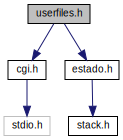
\includegraphics[width=195pt]{userfiles_8h__incl}
\end{center}
\end{figure}
This graph shows which files directly or indirectly include this file\+:
\nopagebreak
\begin{figure}[H]
\begin{center}
\leavevmode
\includegraphics[width=211pt]{userfiles_8h__dep__incl}
\end{center}
\end{figure}
\subsection*{Macros}
\begin{DoxyCompactItemize}
\item 
\#define \hyperlink{userfiles_8h_a698a8661109d5789f2b856cdf3b22adb}{file2estado}(user, flag)~(\hyperlink{userfiles_8h_a9956376d29d551af64f82f7af082ec39}{file2estado\+\_\+un}(\hyperlink{cgi_8h_a2997e8baab88fb20ec0dce822d405aa9}{U\+S\+E\+R\+\_\+\+P\+A\+T\+H},user,\&(flag)))
\begin{DoxyCompactList}\small\item\em Macro para converter um ficheiro em estado. \end{DoxyCompactList}\item 
\#define \hyperlink{userfiles_8h_af94c939d48715fec1933684c3073f7d9}{estado2file}(user, e)~(\hyperlink{userfiles_8h_a2f7763ec29a228279585236b4e3d6252}{estado2file\+\_\+un}(\hyperlink{cgi_8h_a2997e8baab88fb20ec0dce822d405aa9}{U\+S\+E\+R\+\_\+\+P\+A\+T\+H},user,e))
\begin{DoxyCompactList}\small\item\em Macro para converter um estado em ficheiro. \end{DoxyCompactList}\end{DoxyCompactItemize}
\subsection*{Functions}
\begin{DoxyCompactItemize}
\item 
\hyperlink{estado_8c_afbffb4e9c242f93d5a2d607754ce2db8}{E\+S\+T\+A\+D\+O} \hyperlink{userfiles_8h_a9956376d29d551af64f82f7af082ec39}{file2estado\+\_\+un} (char $\ast$path, char $\ast$user, int $\ast$flag)
\begin{DoxyCompactList}\small\item\em Passa um ficheiro para Estado. A função cria um Estado apartir de um ficheiro, assumindo que este está escrito corretamente. É colocado no valor apontador por flag uma represetação nuḿerica da validade do ficheiro lido. \end{DoxyCompactList}\item 
void \hyperlink{userfiles_8h_a2f7763ec29a228279585236b4e3d6252}{estado2file\+\_\+un} (char $\ast$path, char $\ast$user, \hyperlink{estado_8c_afbffb4e9c242f93d5a2d607754ce2db8}{E\+S\+T\+A\+D\+O} e)
\begin{DoxyCompactList}\small\item\em Escreve um estado para ficheiro. \end{DoxyCompactList}\end{DoxyCompactItemize}


\subsection{Detailed Description}
Módulo para conversão entre ficheiros e E\+S\+T\+A\+D\+O. 



\subsection{Macro Definition Documentation}
\hypertarget{userfiles_8h_af94c939d48715fec1933684c3073f7d9}{\index{userfiles.\+h@{userfiles.\+h}!estado2file@{estado2file}}
\index{estado2file@{estado2file}!userfiles.\+h@{userfiles.\+h}}
\subsubsection[{estado2file}]{\setlength{\rightskip}{0pt plus 5cm}\#define estado2file(
\begin{DoxyParamCaption}
\item[{}]{user, }
\item[{}]{e}
\end{DoxyParamCaption}
)~({\bf estado2file\+\_\+un}({\bf U\+S\+E\+R\+\_\+\+P\+A\+T\+H},user,e))}}\label{userfiles_8h_af94c939d48715fec1933684c3073f7d9}


Macro para converter um estado em ficheiro. 


\begin{DoxyParams}{Parameters}
{\em user} & nome de utilizador \\
\hline
{\em e} & estado a guardar \\
\hline
\end{DoxyParams}
\hypertarget{userfiles_8h_a698a8661109d5789f2b856cdf3b22adb}{\index{userfiles.\+h@{userfiles.\+h}!file2estado@{file2estado}}
\index{file2estado@{file2estado}!userfiles.\+h@{userfiles.\+h}}
\subsubsection[{file2estado}]{\setlength{\rightskip}{0pt plus 5cm}\#define file2estado(
\begin{DoxyParamCaption}
\item[{}]{user, }
\item[{}]{flag}
\end{DoxyParamCaption}
)~({\bf file2estado\+\_\+un}({\bf U\+S\+E\+R\+\_\+\+P\+A\+T\+H},user,\&(flag)))}}\label{userfiles_8h_a698a8661109d5789f2b856cdf3b22adb}


Macro para converter um ficheiro em estado. 


\begin{DoxyParams}{Parameters}
{\em user} & nome de utilizador \\
\hline
{\em flag} & Apontador para o inteiro onde irá ser colocado o valor da validade do ficheiro. \\
\hline
\end{DoxyParams}


\subsection{Function Documentation}
\hypertarget{userfiles_8h_a2f7763ec29a228279585236b4e3d6252}{\index{userfiles.\+h@{userfiles.\+h}!estado2file\+\_\+un@{estado2file\+\_\+un}}
\index{estado2file\+\_\+un@{estado2file\+\_\+un}!userfiles.\+h@{userfiles.\+h}}
\subsubsection[{estado2file\+\_\+un}]{\setlength{\rightskip}{0pt plus 5cm}void estado2file\+\_\+un (
\begin{DoxyParamCaption}
\item[{char $\ast$}]{path, }
\item[{char $\ast$}]{user, }
\item[{{\bf E\+S\+T\+A\+D\+O}}]{e}
\end{DoxyParamCaption}
)}}\label{userfiles_8h_a2f7763ec29a228279585236b4e3d6252}


Escreve um estado para ficheiro. 


\begin{DoxyParams}{Parameters}
{\em path} & String correspondente à diretória onde se encontram os users. \\
\hline
{\em user} & String correspondente ao nome do ficheiro que irá ser guardado. \\
\hline
{\em e} & Apontador para o estado que irá ser guardado em ficheiro. \\
\hline
\end{DoxyParams}
fclose(fp); \hypertarget{userfiles_8h_a9956376d29d551af64f82f7af082ec39}{\index{userfiles.\+h@{userfiles.\+h}!file2estado\+\_\+un@{file2estado\+\_\+un}}
\index{file2estado\+\_\+un@{file2estado\+\_\+un}!userfiles.\+h@{userfiles.\+h}}
\subsubsection[{file2estado\+\_\+un}]{\setlength{\rightskip}{0pt plus 5cm}{\bf E\+S\+T\+A\+D\+O} file2estado\+\_\+un (
\begin{DoxyParamCaption}
\item[{char $\ast$}]{path, }
\item[{char $\ast$}]{user, }
\item[{int $\ast$}]{flag}
\end{DoxyParamCaption}
)}}\label{userfiles_8h_a9956376d29d551af64f82f7af082ec39}


Passa um ficheiro para Estado. A função cria um Estado apartir de um ficheiro, assumindo que este está escrito corretamente. É colocado no valor apontador por flag uma represetação nuḿerica da validade do ficheiro lido. 


\begin{DoxyParams}{Parameters}
{\em path} & String correspondente à diretória onde se encontram os users. \\
\hline
{\em user} & String correspondente ao nome do ficheiro que irá ser lido. \\
\hline
{\em flag} & Apontador para o inteiro onde irá ser colocado o valor da validade do ficheiro.\\
\hline
\end{DoxyParams}
\begin{DoxyReturn}{Returns}
O Estado obtido do ficheiro. 
\end{DoxyReturn}

\hypertarget{validate_8c}{\section{validate.\+c File Reference}
\label{validate_8c}\index{validate.\+c@{validate.\+c}}
}


Módulo das funções utilizadas para verificação do tabuleiro.  


{\ttfamily \#include \char`\"{}estado.\+h\char`\"{}}\\*
{\ttfamily \#include \char`\"{}validate.\+h\char`\"{}}\\*
Include dependency graph for validate.\+c\+:
\nopagebreak
\begin{figure}[H]
\begin{center}
\leavevmode
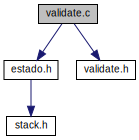
\includegraphics[width=211pt]{validate_8c__incl}
\end{center}
\end{figure}
\subsection*{Macros}
\begin{DoxyCompactItemize}
\item 
\#define \hyperlink{validate_8c_ae3969b94a6cdd703242e3043cc83a0ec}{less\+Col}(j, \hyperlink{structstate}{state})~((j) $<$ (\hyperlink{estado_8h_a4d3c25878918fa5fd1ea3d4a0b1e7a8d}{get\+E\+\_\+cols}(\hyperlink{structstate}{state})))
\begin{DoxyCompactList}\small\item\em Macro utilizada para verificar se o primeiro paramêtro é menor que o número de colunas máximo do estado. \end{DoxyCompactList}\item 
\#define \hyperlink{validate_8c_a80449b0359ced479299462fda9dc9c2e}{less\+Lin}(i, \hyperlink{structstate}{state})~((i) $<$ (\hyperlink{estado_8h_aa3dfd8301c50f971b2d20815617e00d3}{get\+E\+\_\+lins}(\hyperlink{structstate}{state})))
\begin{DoxyCompactList}\small\item\em Macro utilizada para verificar se o primeiro paramêtro é menor que o número de linhas máximo do estado. \end{DoxyCompactList}\item 
\#define \hyperlink{validate_8c_a04580bc5cd9cff271e78e4d5645ed293}{ignore}(i, j, \hyperlink{structstate}{state})~(\hyperlink{estado_8h_ae4aeab324373aa7d36cd03ad28caae57}{get\+E\+\_\+elem}(\hyperlink{structstate}{state}, i, j) != V\+A\+Z\+I\+A \&\& \hyperlink{estado_8h_ae4aeab324373aa7d36cd03ad28caae57}{get\+E\+\_\+elem}(\hyperlink{structstate}{state}, i, j) != B\+L\+O\+Q\+U\+E\+A\+D\+A)
\begin{DoxyCompactList}\small\item\em Macro utilizada para ignorar os casos em que a peça em questão é {\ttfamily V\+A\+Z\+I\+A} ou {\ttfamily B\+L\+O\+Q\+U\+E\+A\+D\+A} . \end{DoxyCompactList}\item 
\#define \hyperlink{validate_8c_ab85e5e9750b691e416c597c0ef25847c}{equals}(num1, num2)~((num1 == num2) $\vert$$\vert$ (num1 == num2 + 3) $\vert$$\vert$ (num1 == num2 -\/ 3))
\begin{DoxyCompactList}\small\item\em Macro verifica se dois valores são equivalentes. Dois valores são equivalentes neste cenário, quando são iguais ou se representarem fixos e soltos. \end{DoxyCompactList}\item 
\#define \hyperlink{validate_8c_ad3ddaa88cdf36ed91ed86c882719b023}{equal}(i1, j1, i2, j2, \hyperlink{structstate}{state})~(\hyperlink{validate_8c_ab85e5e9750b691e416c597c0ef25847c}{equals}(\hyperlink{estado_8h_ae4aeab324373aa7d36cd03ad28caae57}{get\+E\+\_\+elem}(\hyperlink{structstate}{state}, i1, j1), \hyperlink{estado_8h_ae4aeab324373aa7d36cd03ad28caae57}{get\+E\+\_\+elem}(\hyperlink{structstate}{state}, i2, j2)))
\begin{DoxyCompactList}\small\item\em Macro que passa argumentos para a Macro equals segundo valores obtidos do {\ttfamily E\+S\+T\+A\+D\+O}. \end{DoxyCompactList}\item 
\#define \hyperlink{validate_8c_ae73a74cf98c9a84b845a218034c8e274}{countval}(i1, j1, i2, j2, \hyperlink{structstate}{state})~(\hyperlink{validate_8c_ad3ddaa88cdf36ed91ed86c882719b023}{equal}(i1, j1, i2, j2, \hyperlink{structstate}{state}) \&\& \hyperlink{validate_8c_a04580bc5cd9cff271e78e4d5645ed293}{ignore}(i1, j1, \hyperlink{structstate}{state}))
\begin{DoxyCompactList}\small\item\em Macro utilizada para a verificação da validade de uma sequência de peças. Comando 'countval' é utilizado para ignorar peças bloqueadas ou vazias e confirmar se a peça seguinte à atual é válida, incluindo para fixos, ou não. \end{DoxyCompactList}\item 
\#define \hyperlink{validate_8c_a3e83cfe59dc3bacf9951d6e40cb4ecc7}{testall}(i, j, \hyperlink{structstate}{state})~((\hyperlink{validate_8c_a80449b0359ced479299462fda9dc9c2e}{less\+Lin}(i, \hyperlink{structstate}{state})) \&\& (\hyperlink{validate_8c_ae3969b94a6cdd703242e3043cc83a0ec}{less\+Col}(j, \hyperlink{structstate}{state})) \&\& (i $>$= 0) \&\& (j $>$= 0))
\begin{DoxyCompactList}\small\item\em Macro utilizada para restringir as váriaveis aos limites da grelha. \end{DoxyCompactList}\item 
\#define \hyperlink{validate_8c_a2eb737617082e5efeb996b6e36fb3fd0}{contain}(i1, j1, i2, j2, \hyperlink{structstate}{state})~(\hyperlink{validate_8c_a3e83cfe59dc3bacf9951d6e40cb4ecc7}{testall}(i1, j1, \hyperlink{structstate}{state}) \&\& \hyperlink{validate_8c_a3e83cfe59dc3bacf9951d6e40cb4ecc7}{testall}(i2, j2, \hyperlink{structstate}{state}))
\begin{DoxyCompactList}\small\item\em Macro que passa argumentos à macro testall de forma restringir dois elementos. \end{DoxyCompactList}\end{DoxyCompactItemize}
\subsection*{Functions}
\begin{DoxyCompactItemize}
\item 
int \hyperlink{validate_8c_a7cc26aa61c34f0e7fd569e7e176ef8e4}{valtab} (\hyperlink{estado_8c_afbffb4e9c242f93d5a2d607754ce2db8}{E\+S\+T\+A\+D\+O} \hyperlink{structstate}{state}, int i, int j)
\begin{DoxyCompactList}\small\item\em Verifica se uma posição na grelha do estado passado, é válida (Ou seja, não possui 3 em linhas em nenhuma direção). \end{DoxyCompactList}\item 
static int \hyperlink{validate_8c_a41577d63c98a897565c29142cecd6f13}{validside} (int i, int j, int vectori, int vectorj, \hyperlink{estado_8c_afbffb4e9c242f93d5a2d607754ce2db8}{E\+S\+T\+A\+D\+O} \hyperlink{structstate}{state})
\begin{DoxyCompactList}\small\item\em Verifica se dado um vetor uma posição é válida no estado. A função segue a trajetória indicada pelo vetor passado, bem como no sentido aposto a este. Utilizando para tal as macros {\ttfamily contain} e {\ttfamily countval} para obter a contagem de elementos iguais segundo a direção do {\bfseries vetor} passado como argumento. \end{DoxyCompactList}\end{DoxyCompactItemize}


\subsection{Detailed Description}
Módulo das funções utilizadas para verificação do tabuleiro. 



\subsection{Macro Definition Documentation}
\hypertarget{validate_8c_a2eb737617082e5efeb996b6e36fb3fd0}{\index{validate.\+c@{validate.\+c}!contain@{contain}}
\index{contain@{contain}!validate.\+c@{validate.\+c}}
\subsubsection[{contain}]{\setlength{\rightskip}{0pt plus 5cm}\#define contain(
\begin{DoxyParamCaption}
\item[{}]{i1, }
\item[{}]{j1, }
\item[{}]{i2, }
\item[{}]{j2, }
\item[{}]{{\bf state}}
\end{DoxyParamCaption}
)~({\bf testall}(i1, j1, {\bf state}) \&\& {\bf testall}(i2, j2, {\bf state}))}}\label{validate_8c_a2eb737617082e5efeb996b6e36fb3fd0}


Macro que passa argumentos à macro testall de forma restringir dois elementos. 


\begin{DoxyParams}{Parameters}
{\em i1} & Linha do primeiro elemento a restringir. \\
\hline
{\em j1} & Coluna do primeiro elemento a restringir. \\
\hline
{\em i2} & Linha do segundo elemento a restringir. \\
\hline
{\em j2} & Coluna do segundo elemento a restringir. \\
\hline
{\em state} & Estado do qual se pretende obter os valores de restrição. \\
\hline
\end{DoxyParams}
\hypertarget{validate_8c_ae73a74cf98c9a84b845a218034c8e274}{\index{validate.\+c@{validate.\+c}!countval@{countval}}
\index{countval@{countval}!validate.\+c@{validate.\+c}}
\subsubsection[{countval}]{\setlength{\rightskip}{0pt plus 5cm}\#define countval(
\begin{DoxyParamCaption}
\item[{}]{i1, }
\item[{}]{j1, }
\item[{}]{i2, }
\item[{}]{j2, }
\item[{}]{{\bf state}}
\end{DoxyParamCaption}
)~({\bf equal}(i1, j1, i2, j2, {\bf state}) \&\& {\bf ignore}(i1, j1, {\bf state}))}}\label{validate_8c_ae73a74cf98c9a84b845a218034c8e274}


Macro utilizada para a verificação da validade de uma sequência de peças. Comando 'countval' é utilizado para ignorar peças bloqueadas ou vazias e confirmar se a peça seguinte à atual é válida, incluindo para fixos, ou não. 


\begin{DoxyParams}{Parameters}
{\em i1} & Linha do primeiro elemento. \\
\hline
{\em j1} & Coluna do primeiro elemento. \\
\hline
{\em i2} & Linha do segundo elemento. \\
\hline
{\em j2} & Coluna do segundo elemento. \\
\hline
{\em state} & {\ttfamily E\+S\+T\+A\+D\+O} onde se encontram os elementos a comparar.\\
\hline
\end{DoxyParams}
\begin{DoxySeeAlso}{See also}
\hyperlink{validate_8c_ad3ddaa88cdf36ed91ed86c882719b023}{equal} 

\hyperlink{validate_8c_a04580bc5cd9cff271e78e4d5645ed293}{ignore} 
\end{DoxySeeAlso}
\hypertarget{validate_8c_ad3ddaa88cdf36ed91ed86c882719b023}{\index{validate.\+c@{validate.\+c}!equal@{equal}}
\index{equal@{equal}!validate.\+c@{validate.\+c}}
\subsubsection[{equal}]{\setlength{\rightskip}{0pt plus 5cm}\#define equal(
\begin{DoxyParamCaption}
\item[{}]{i1, }
\item[{}]{j1, }
\item[{}]{i2, }
\item[{}]{j2, }
\item[{}]{{\bf state}}
\end{DoxyParamCaption}
)~({\bf equals}({\bf get\+E\+\_\+elem}({\bf state}, i1, j1), {\bf get\+E\+\_\+elem}({\bf state}, i2, j2)))}}\label{validate_8c_ad3ddaa88cdf36ed91ed86c882719b023}


Macro que passa argumentos para a Macro equals segundo valores obtidos do {\ttfamily E\+S\+T\+A\+D\+O}. 


\begin{DoxyParams}{Parameters}
{\em i1} & Linha do primeiro elemento \\
\hline
{\em j1} & Coluna do primeiro elemento \\
\hline
{\em i2} & Linha do segundo elemento \\
\hline
{\em j2} & Coluna do segundo elemento \\
\hline
{\em state} & {\ttfamily E\+S\+T\+A\+D\+O} onde se encontram os elementos a comparar\\
\hline
\end{DoxyParams}
\begin{DoxyReturn}{Returns}
Se os elementos forem iguais retorna 1, caso contrário devolve 0.
\end{DoxyReturn}
\begin{DoxySeeAlso}{See also}
\hyperlink{validate_8c_ab85e5e9750b691e416c597c0ef25847c}{equals} 
\end{DoxySeeAlso}
\hypertarget{validate_8c_ab85e5e9750b691e416c597c0ef25847c}{\index{validate.\+c@{validate.\+c}!equals@{equals}}
\index{equals@{equals}!validate.\+c@{validate.\+c}}
\subsubsection[{equals}]{\setlength{\rightskip}{0pt plus 5cm}\#define equals(
\begin{DoxyParamCaption}
\item[{}]{num1, }
\item[{}]{num2}
\end{DoxyParamCaption}
)~((num1 == num2) $\vert$$\vert$ (num1 == num2 + 3) $\vert$$\vert$ (num1 == num2 -\/ 3))}}\label{validate_8c_ab85e5e9750b691e416c597c0ef25847c}


Macro verifica se dois valores são equivalentes. Dois valores são equivalentes neste cenário, quando são iguais ou se representarem fixos e soltos. 


\begin{DoxyParams}{Parameters}
{\em num1} & Primeiro valor do tabuleiro a ser verificado. \\
\hline
{\em num2} & Segundo valor do tabuleiro a ser verificado.\\
\hline
\end{DoxyParams}
\begin{DoxyReturn}{Returns}
Se os dois valores forem equivalente devolve 1, caso contrário devolve 0. 
\end{DoxyReturn}
\hypertarget{validate_8c_a04580bc5cd9cff271e78e4d5645ed293}{\index{validate.\+c@{validate.\+c}!ignore@{ignore}}
\index{ignore@{ignore}!validate.\+c@{validate.\+c}}
\subsubsection[{ignore}]{\setlength{\rightskip}{0pt plus 5cm}\#define ignore(
\begin{DoxyParamCaption}
\item[{}]{i, }
\item[{}]{j, }
\item[{}]{{\bf state}}
\end{DoxyParamCaption}
)~({\bf get\+E\+\_\+elem}({\bf state}, i, j) != V\+A\+Z\+I\+A \&\& {\bf get\+E\+\_\+elem}({\bf state}, i, j) != B\+L\+O\+Q\+U\+E\+A\+D\+A)}}\label{validate_8c_a04580bc5cd9cff271e78e4d5645ed293}


Macro utilizada para ignorar os casos em que a peça em questão é {\ttfamily V\+A\+Z\+I\+A} ou {\ttfamily B\+L\+O\+Q\+U\+E\+A\+D\+A} . 


\begin{DoxyParams}{Parameters}
{\em i} & Linha do elemento. \\
\hline
{\em j} & Coluna do elemento. \\
\hline
{\em state} & Estado do qual se pretende obter a informação. \\
\hline
\end{DoxyParams}
\hypertarget{validate_8c_ae3969b94a6cdd703242e3043cc83a0ec}{\index{validate.\+c@{validate.\+c}!less\+Col@{less\+Col}}
\index{less\+Col@{less\+Col}!validate.\+c@{validate.\+c}}
\subsubsection[{less\+Col}]{\setlength{\rightskip}{0pt plus 5cm}\#define less\+Col(
\begin{DoxyParamCaption}
\item[{}]{j, }
\item[{}]{{\bf state}}
\end{DoxyParamCaption}
)~((j) $<$ ({\bf get\+E\+\_\+cols}({\bf state})))}}\label{validate_8c_ae3969b94a6cdd703242e3043cc83a0ec}


Macro utilizada para verificar se o primeiro paramêtro é menor que o número de colunas máximo do estado. 


\begin{DoxyParams}{Parameters}
{\em j} & Componente das abcissas de uma posição. \\
\hline
{\em state} & Estado utilizado para verificar o número de colunas máximo. \\
\hline
\end{DoxyParams}
\hypertarget{validate_8c_a80449b0359ced479299462fda9dc9c2e}{\index{validate.\+c@{validate.\+c}!less\+Lin@{less\+Lin}}
\index{less\+Lin@{less\+Lin}!validate.\+c@{validate.\+c}}
\subsubsection[{less\+Lin}]{\setlength{\rightskip}{0pt plus 5cm}\#define less\+Lin(
\begin{DoxyParamCaption}
\item[{}]{i, }
\item[{}]{{\bf state}}
\end{DoxyParamCaption}
)~((i) $<$ ({\bf get\+E\+\_\+lins}({\bf state})))}}\label{validate_8c_a80449b0359ced479299462fda9dc9c2e}


Macro utilizada para verificar se o primeiro paramêtro é menor que o número de linhas máximo do estado. 


\begin{DoxyParams}{Parameters}
{\em i} & Componente das abcissas de uma posição. \\
\hline
{\em state} & Estado utilizado para verificar o número de linhas máximo. \\
\hline
\end{DoxyParams}
\hypertarget{validate_8c_a3e83cfe59dc3bacf9951d6e40cb4ecc7}{\index{validate.\+c@{validate.\+c}!testall@{testall}}
\index{testall@{testall}!validate.\+c@{validate.\+c}}
\subsubsection[{testall}]{\setlength{\rightskip}{0pt plus 5cm}\#define testall(
\begin{DoxyParamCaption}
\item[{}]{i, }
\item[{}]{j, }
\item[{}]{{\bf state}}
\end{DoxyParamCaption}
)~(({\bf less\+Lin}(i, {\bf state})) \&\& ({\bf less\+Col}(j, {\bf state})) \&\& (i $>$= 0) \&\& (j $>$= 0))}}\label{validate_8c_a3e83cfe59dc3bacf9951d6e40cb4ecc7}


Macro utilizada para restringir as váriaveis aos limites da grelha. 


\begin{DoxyParams}{Parameters}
{\em i} & Linha a restringir. \\
\hline
{\em j} & Coluna a restringir. \\
\hline
{\em state} & Estado do qual se pretende obter os valores de restrição. \\
\hline
\end{DoxyParams}


\subsection{Function Documentation}
\hypertarget{validate_8c_a41577d63c98a897565c29142cecd6f13}{\index{validate.\+c@{validate.\+c}!validside@{validside}}
\index{validside@{validside}!validate.\+c@{validate.\+c}}
\subsubsection[{validside}]{\setlength{\rightskip}{0pt plus 5cm}static int validside (
\begin{DoxyParamCaption}
\item[{int}]{i, }
\item[{int}]{j, }
\item[{int}]{vectori, }
\item[{int}]{vectorj, }
\item[{{\bf E\+S\+T\+A\+D\+O}}]{state}
\end{DoxyParamCaption}
)\hspace{0.3cm}{\ttfamily [static]}}}\label{validate_8c_a41577d63c98a897565c29142cecd6f13}


Verifica se dado um vetor uma posição é válida no estado. A função segue a trajetória indicada pelo vetor passado, bem como no sentido aposto a este. Utilizando para tal as macros {\ttfamily contain} e {\ttfamily countval} para obter a contagem de elementos iguais segundo a direção do {\bfseries vetor} passado como argumento. 


\begin{DoxyParams}{Parameters}
{\em j} & representa a coluna que se pretende verificar. \\
\hline
{\em i} & representa a linha que se pretende verificar. \\
\hline
{\em vectori} & representa a componente das linhas do vetor utilizado. \\
\hline
{\em vectorj} & representa a componente das colunas do vetor utilizado. \\
\hline
{\em state} & Estado do qual se pretende analisar a grelha.\\
\hline
\end{DoxyParams}
\begin{DoxyReturn}{Returns}
Quantas peças do mesmo valor há à volta de uma certa posição, segundo a direção do vetor.
\end{DoxyReturn}
\begin{DoxySeeAlso}{See also}
\hyperlink{validate_8c_a2eb737617082e5efeb996b6e36fb3fd0}{contain} 

\hyperlink{validate_8c_ae73a74cf98c9a84b845a218034c8e274}{countval} 
\end{DoxySeeAlso}
\hypertarget{validate_8c_a7cc26aa61c34f0e7fd569e7e176ef8e4}{\index{validate.\+c@{validate.\+c}!valtab@{valtab}}
\index{valtab@{valtab}!validate.\+c@{validate.\+c}}
\subsubsection[{valtab}]{\setlength{\rightskip}{0pt plus 5cm}int valtab (
\begin{DoxyParamCaption}
\item[{{\bf E\+S\+T\+A\+D\+O}}]{state, }
\item[{int}]{i, }
\item[{int}]{j}
\end{DoxyParamCaption}
)}}\label{validate_8c_a7cc26aa61c34f0e7fd569e7e176ef8e4}


Verifica se uma posição na grelha do estado passado, é válida (Ou seja, não possui 3 em linhas em nenhuma direção). 


\begin{DoxyParams}{Parameters}
{\em i} & Linha que se pretende verificar. \\
\hline
{\em j} & Coluna que se pretende verificar. \\
\hline
{\em state} & Apontador para o estado que possui a grelha onde se pretende avaliar a posição.\\
\hline
\end{DoxyParams}
\begin{DoxyReturn}{Returns}
Validade da posição na grelha.
\end{DoxyReturn}
\begin{DoxySeeAlso}{See also}
\hyperlink{validate_8c_a41577d63c98a897565c29142cecd6f13}{validside} 
\end{DoxySeeAlso}

\hypertarget{validate_8h}{\section{validate.\+h File Reference}
\label{validate_8h}\index{validate.\+h@{validate.\+h}}
}


Módulo de funções utilizadas para verificação do tabuleiro.  


This graph shows which files directly or indirectly include this file\+:
\nopagebreak
\begin{figure}[H]
\begin{center}
\leavevmode
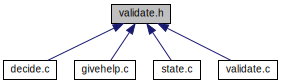
\includegraphics[width=350pt]{validate_8h__dep__incl}
\end{center}
\end{figure}
\subsection*{Functions}
\begin{DoxyCompactItemize}
\item 
int \hyperlink{validate_8h_a7cc26aa61c34f0e7fd569e7e176ef8e4}{valtab} (\hyperlink{estado_8c_afbffb4e9c242f93d5a2d607754ce2db8}{E\+S\+T\+A\+D\+O} \hyperlink{structstate}{state}, int i, int j)
\begin{DoxyCompactList}\small\item\em Verifica se uma posição na grelha do estado passado, é válida (Ou seja, não possui 3 em linhas em nenhuma direção). \end{DoxyCompactList}\end{DoxyCompactItemize}


\subsection{Detailed Description}
Módulo de funções utilizadas para verificação do tabuleiro. 



\subsection{Function Documentation}
\hypertarget{validate_8h_a7cc26aa61c34f0e7fd569e7e176ef8e4}{\index{validate.\+h@{validate.\+h}!valtab@{valtab}}
\index{valtab@{valtab}!validate.\+h@{validate.\+h}}
\subsubsection[{valtab}]{\setlength{\rightskip}{0pt plus 5cm}int valtab (
\begin{DoxyParamCaption}
\item[{{\bf E\+S\+T\+A\+D\+O}}]{state, }
\item[{int}]{i, }
\item[{int}]{j}
\end{DoxyParamCaption}
)}}\label{validate_8h_a7cc26aa61c34f0e7fd569e7e176ef8e4}


Verifica se uma posição na grelha do estado passado, é válida (Ou seja, não possui 3 em linhas em nenhuma direção). 


\begin{DoxyParams}{Parameters}
{\em i} & Linha que se pretende verificar. \\
\hline
{\em j} & Coluna que se pretende verificar. \\
\hline
{\em state} & Apontador para o estado que possui a grelha onde se pretende avaliar a posição.\\
\hline
\end{DoxyParams}
\begin{DoxyReturn}{Returns}
Validade da posição na grelha.
\end{DoxyReturn}
\begin{DoxySeeAlso}{See also}
\hyperlink{validate_8c_a41577d63c98a897565c29142cecd6f13}{validside} 
\end{DoxySeeAlso}

%--- End generated contents ---

% Index
\newpage
\phantomsection
\addcontentsline{toc}{chapter}{Index}
\printindex

\end{document}
